\documentclass[a4paper,twoside]{report}
\usepackage{geometry}
\usepackage{hyperref}
\usepackage[textsize=tiny]{todonotes}
%\usepackage{etex}
\usepackage[all]{xy}
\SelectTips{cm}{}
% derivations and labels
\usepackage{proof}
\newcommand{\lab}[1]{\ensuremath{\mathsf{{#1}}}}
\newcommand{\slab}[1]{\ensuremath{\scriptstyle{\mathsf{{#1}}}}}

\newcommand{\sub}[3]{{\mathcal{#1}}\textrm{-}\mathsf{Sub}_{\textbf {\textup{#2}}}(#3)}

\newcommand{\msub}[2]{\mathsf{Sub}_{\textbf {\textup{#1}}}(#2)}

%frecce
\newcommand{\mor}{\mathsf{Mor}}
\newcommand{\mon}{\mathsf{Mono}}
\newcommand{\reg}{\mathsf{Reg}}

% ``boxed'' \infer command
\newcommand{\binfer}[3][]{
  \mbox{\infer[#1]{#2}{#3}}}

% Command for labels on the left side of the rule
%       \inferL{<name>}{<post>}{<pre>}
% generates:
%             <pre>
%      <name> ------
%             <post>
%
\newlength{\myheight}
\newcommand{\inferL}[3]
  {\settoheight{\myheight}{\mbox{${#2}$}}
   \raisebox{\myheight}{{#1}}
   \makebox[1mm]{}
   \mbox{\infer{#2}{#3}}
}

\usepackage{amssymb,graphicx,epsfig,color}
%\usepackage[scriptsize]{subfigure}
\usepackage{subcaption}
\usepackage{wrapfig}

% re-stating 
%\usepackage{thm-restate}

% showing labels
%\usepackage[inline]{showlabels}

\usepackage{pgf}
\usepackage{tikz}
\usepackage{tikz-cd}
\usetikzlibrary{arrows,shapes,snakes,automata,backgrounds,petri,fit,positioning,calc}
\tikzstyle{node}=[circle, draw=black, minimum size=1mm, inner sep=1.5pt, font=\tiny]

\tikzstyle{trans}=[font=\scriptsize]
\tikzstyle{lab}=[font=\small]
\tikzset{
	coloredge/.style={
		->,
		color=red
		%densely dotted
	}
}

\tikzset{
	colorloop/.style={
		loop,
		color=red
		%densely dotted
	}
}

\tikzcdset{
	perm/.style={
		shorten >=-1mm, shorten <=-1mm,
		-,
		% dotted
	}
}

\newcommand{\pgfBox}{
  \begin{pgfonlayer}{background} 
    \fill[blue!2,thick,draw=black!50,rounded corners,inner sep=3mm] ([xshift=-1.5pt,yshift=-1.5pt]current bounding box.south west) rectangle ([xshift=1.5pt,yshift=1.5pt]current bounding box.north east);
  \end{pgfonlayer}
}
\usepackage{scalerel}
\newcommand{\smallmin}{\scaleobj{0.6}{-}}
\newcommand{\Deltamin}{\Delta^{\hspace{-1pt}\downarrow\hspace{-1pt}}}
\newcommand{\Rrel}[1]   {\stackrel{{#1}}{\Longrightarrow}}
\newcommand{\oa}{\overline a}
\newcommand{\ob}{\overline b}
\newcommand{\oc}{\overline c}
\newcommand{\od}{\overline d}
\newcommand{\rec}{\emph{rec}}
\newcommand{\fn}[1]{{\mathtt{fn}}(#1)}
%\usepackage{latexsym}
\usepackage{stmaryrd}
\def\encodep#1{\llfloor#1\rrfloor}

\newcommand{\cat}[1]{\ensuremath{\mathbf{#1}}}

\newcommand{\dpo}{\textsc{dpo}}

% base classes of categories for adhesive and quasi adhesive case
\newcommand{\bAdh}{\ensuremath{\mathbb{B}}}
\newcommand{\bQAdh}{\ensuremath{\mathbb{QB}}}

%from pawel
\usepackage[latin1]{inputenc}
\usepackage{amsmath}

\usepackage{amssymb}
\usepackage{amsthm}
\usepackage{enumerate}
\usepackage{xspace}
\usepackage{amsfonts}
\usepackage{mathrsfs}
\usepackage{cite}
\usepackage{float}
\usepackage{fancybox}

\usepackage{cleveref}


%\spnewtheorem*{notation}{Notation}{\bfseries}{\rmfamily}

%%%%%%%% MATHEMATICAL NOTATION %%%%%%%%%%%%%%%%%%%%%%%%%%%%%%%%%%%%%%%%%

%symbol for natural numbers
\newcommand{\nat}{\ensuremath{\mathbb{N}}}

% finite subset
\newcommand{\sfin}{\ensuremath{\subseteq_{\mathit{fin}}}}

% flattening of a multiset
\newcommand{\flt}[1]{\ensuremath{[\![{#1}]\!]}}

% compact elements
\newcommand{\compact}[1]{\ensuremath{\mathop{\mathsf{K}({#1})}}}

% principal ideal
\newcommand{\principal}[1]{\ensuremath{\mathop{\downarrow\!{#1}}}}

% ideal completion
\newcommand{\ideal}[1]{\ensuremath{\mathsf{Idl}({#1})}}

% complete prime elements
\newcommand{\pr}[1]{\ensuremath{\mathop{\mathit{pr}({#1})}}}
\newcommand{\wpr}[1]{\ensuremath{\mathop{\mathit{wpr}({#1})}}}

% irreducible elements
\newcommand{\ir}[1]{\ensuremath{\mathop{\mathit{ir}({#1})}}}

% difference of irreducible elements
\newcommand{\diff}[2]{\ensuremath{\delta({#1},{#2})}}

% immediate precedence

% abbreviation for event structure
% \newcommand{\esabbr}{event structure}
\newcommand{\esabbr}{\textsc{es}}
\newcommand{\esnabbr}{\textsc{esnb}}
\newcommand{\esnmabbr}{\textsc{esn}}
\newcommand{\eseqabbr}{\textsc{epes}}

% predecessor of an irreducible
\newcommand{\pred}[1]{\ensuremath{\mathit{p}({#1})}}

% irreducible elements in es domains
\newcommand{\esir}[2]{\ensuremath{\langle{#1}, {#2}\rangle}}

% equivalence classes [of irreducibles]
\newcommand{\eqclass}[2][]{\ensuremath{[{#2}]_{\scriptscriptstyle {#1}}}}
% union of the equivalence classes of the elements in a set
\newcommand{\eqclasscup}[2]{\ensuremath{{#2}_{\scriptscriptstyle {#1}}}}

\newcommand{\eqclassir}[1]{\ensuremath{\eqclass[\leftrightarrow^*]{#1}}}

% quotient of set wrt a relation
\newcommand{\quotient}[2]{\ensuremath{{#1}_{\scriptscriptstyle {#2}}}}

% category of event structures 
\newcommand{\es}{\ensuremath{\mathsf{ES}}}
% category of stable event structures 
\newcommand{\ses}{\ensuremath{\mathsf{sES}}}
% category of prime event structures 
\newcommand{\pes}{\ensuremath{\mathsf{pES}}}
% category of prime event structures with equivalence
\newcommand{\epes}{\ensuremath{\mathsf{epES}}}

% category of connected event structures 
\newcommand{\ces}{\ensuremath{\mathsf{cES}}}

% category of weak prime algebraic domains domains 
\newcommand{\WDom}{\ensuremath{\mathsf{wDom}}}
% category of domains
\newcommand{\Dom}{\ensuremath{\mathsf{Dom}}}
% category of prime algebraic domains
\newcommand{\PDom}{\ensuremath{\mathsf{pDom}}}


%%%%% NON BINARY CONFLICT

% category of event structures 
\newcommand{\esn}{\ensuremath{\mathsf{ES_{nb}}}}
% category of stable event structures 
\newcommand{\sesn}{\ensuremath{\mathsf{sES_n}}}

% category of connected event structures 
\newcommand{\cesn}{\ensuremath{\mathsf{cES_{nb}}}}

% category of prime event structures 
\newcommand{\pesn}{\ensuremath{\mathsf{pES_n}}}

% category of fusion domains 
\newcommand{\WDomb}{\ensuremath{\mathsf{wDom_b}}}
% category of domains
\newcommand{\Domb}{\ensuremath{\mathsf{Dom_b}}}
% category of prime algebraic domains
\newcommand{\PDomb}{\ensuremath{\mathsf{pDom_b}}}

%%%%% END NON BINARY CONFLICT


% slice category
\newcommand{\slice}[2]{\ensuremath{({#1} \downarrow {#2})}}


% event structure for a domain
\newcommand{\zev}[0]{\ensuremath{\mathcal{E}}}
\newcommand{\ev}[1]{\ensuremath{\zev({#1})}}

% from general to connected event structures
\newcommand{\zconnes}[0]{\ensuremath{\mathcal{C}}}
\newcommand{\connes}[1]{\ensuremath{\zconnes({#1})}}
% and inclusion
\newcommand{\zinces}[0]{\ensuremath{\mathcal{I}}}
\newcommand{\inces}[1]{\ensuremath{\zinces({#1})}}


% stable version
\newcommand{\zsev}[0]{\ensuremath{\mathcal{E}_S}}
\newcommand{\sev}[1]{\ensuremath{\zsev({#1})}}

% with equivalence
\newcommand{\zeveq}[0]{\ensuremath{\mathcal{E}_{eq}}}
\newcommand{\eveq}[1]{\ensuremath{\zeveq({#1})}}

% es with equivalence to es and vice
\newcommand{\zfuse}[0]{\ensuremath{\mathcal{M}}}
\newcommand{\fuse}[1]{\ensuremath{\zfuse({#1})}}
\newcommand{\zunf}[0]{\ensuremath{\zunf}}
\newcommand{\unf}[1]{\ensuremath{\mathcal{U}({#1})}}

\newcommand{\gph}[1]{\textbf{\textup{{#1}-Graph}}}


% Winskel/Droste version
\newcommand{\zevwd}[0]{\ensuremath{\mathcal{E}_{wd}}}
\newcommand{\evwd}[1]{\ensuremath{\zevwd({#1})}}




% configurations of an event structure
\newcommand{\conf}[1]{\ensuremath{\mathit{Conf}({#1})}}
% finite configurations
\newcommand{\conff}[1]{\ensuremath{\mathit{Conf_F}({#1})}}

% product of the sets of minimal enablinsg
\newcommand{\pmin}[1]{\ensuremath{U_{#1}}}

% connectectedness of minimal enablinsg
\newcommand{\conn}[1]{\ensuremath{\stackrel{#1}{\frown}}}


% domain for an event structure or graph grammar
\newcommand{\zdom}[0]{\ensuremath{\mathcal{D}}}
\newcommand{\dom}[1]{\ensuremath{\zdom({#1})}}


\newcommand{\zdomeq}[0]{\ensuremath{\mathcal{D}_{eq}}}
\newcommand{\domeq}[1]{\ensuremath{\zdomeq({#1})}}


% partial order for a graph grammar
\newcommand{\poset}[1]{\ensuremath{\mathcal{P}({#1})}}

% stable version
\newcommand{\pdom}[1]{\ensuremath{\mathcal{D}_S({#1})}}
\newcommand{\ppdom}[0]{\ensuremath{\mathcal{D}_S}}


% powerset
\newcommand{\Pow}[1]{\ensuremath{\mathbf{2}^{#1}}}

% powerset of finite subsets
\newcommand{\Powfin}[1]{\ensuremath{\mathbf{2}_\mathit{fin}^{#1}}}

% powerset of subsets of cardinality <= 1
\newcommand{\Powone}[1]{\ensuremath{\mathbf{2}_1^{#1}}}

% integer interval
\newcommand{\interval}[2][1]{\ensuremath{[{#1},{#2}]}}

% domain interval
\newcommand{\dint}[2]{\ensuremath{[{#1},{#2}]}}

% set of intervals
\newcommand{\IntSet}[1]{\ensuremath{\mathop{\mathit{Int}({#1})}}}

% intervals to irreducibles and vice
\newcommand{\inir}{\ensuremath{\mathop{\mathit{\zeta}}}}
\newcommand{\irin}{\ensuremath{\mathop{\mathit{\iota}}}}

% permutations
\newcommand{\perm}{\sigma}

% causes
\newcommand{\causes}[1]{\ensuremath{\lfloor {#1})}}

%%% GRAPH GRAMMARS


\newcommand{\Abs}[1]{\ensuremath{\mathsf{Abs}({#1})}}
\newcommand{\tr}[1]{\ensuremath{\mathsf{Tr}({#1})}}
% fusion safe traces
\newcommand{\trs}[1]{\ensuremath{\mathsf{Tr}_s({#1})}}
%\newcommand{\graph}{\ensuremath{\mathsf{Graph}}}
\newcommand{\tgraph}[1]{\ensuremath{\mathsf{Graph}_{#1}}}
\newcommand{\can}[1]{\ensuremath{\mathsf{C}({#1})}}
% source and target of a derivation
\newcommand{\source}[1]{\ensuremath{\mathsf{s}({#1})}}
\newcommand{\target}[1]{\ensuremath{\mathsf{t}({#1})}}
\newcommand{\col}[1]{\ensuremath{\mathsf{col}({#1})}}

% left decorated trace
\newcommand{\ltrace}[1]{\ensuremath{\langle {#1}\rangle_c}}

\newcommand{\bx}[1]{\phantom{\big(}#1{\phantom{\big)}}}
\newcommand{\bxx}[1]{\,#1\,}
\newcommand{\cycl}[1]{\ensuremath{\mbox{\textcircled{\scriptsize{$#1$}}}}}
\renewcommand{\iff}{\ensuremath{\Leftrightarrow}}

%%%%GENERAL CATEGORICAL NOTATION

%identità
\newcommand{\id}[1]{\mathsf{id}_{#1}}
%codominio
\newcommand{\cod}[1]{\mathsf{cod}({#1})}
	%Variabili categorie
\def\A{\textbf {\textup{A}}}
%mono
\newcommand{\mto}[0]{\scalebox{1}{$\rightarrowtail$}}


\newcommand{\sk}{\mathsf{sk}_{\X}}


\def\R{\mathsf{R}}
\def\B{\textbf {\textup{B}}}
\def\C{\textbf {\textup{C}}}
\def\D{\textbf {\textup{D}}}
\def\X{\textbf {\textup{X}}}
\def\Y{\textbf {\textup{Y}}}
\def\E{\textbf {\textup{E}}}

\newcommand{\ske}{\mathsf{sk}(\X)}
\renewcommand{\P}{\textbf {\textup{P}}}

%\derivazioni

\newcommand{\dder}[1]{\mathscr{#1}}
\newcommand{\sder}[2]{S_{i_1,i_2}(\mathscr{#1}, \mathscr{#2})}
\newcommand{\der}[1]{\underline{\dder{#1}}}
\def\dpo{\mathsf{C}^{\X}_R}
\def\gpo{\mathsf{G}^{\X}_R}
\def\dpi{[\mathsf{C}]^{\X}_R}
\def\gpi{[\mathsf{G}]^{\X}_R}

\newcommand{\ider}[1]{\mathscr{I}_{#1}}

%categorie
\def\Set{\textbf {\textup{Set}}}

%comma
\newcommand{\comma}[2]{#1\hspace{1pt} {\downarrow}\hspace{1pt} #2}
\newcommand{\cma}[2]{\mathcal{#1}\hspace{1pt} {\downarrow}\hspace{1pt} \mathcal{#2}}

%derivazioni
\newcommand{\lpro}{\langle \hspace{-1.85pt}[}
\newcommand{\rpro}{]\hspace{-1.85pt}\rangle}
\newcommand{\tpro}[1]{\lpro \der{#1}\rpro}
\newcommand{\tproi}[2]{\lpro \der{#1}_{#2}\rpro}
\newcommand{\lgh}[0]{\mathsf{lg}}

%%% NEW

\usepackage{xparse}

% inversions
\newcommand{\inv}[1]{\ensuremath{inv}({#1})}

% direct shift
\newcommand{\shiftdir}[1][]{\ensuremath{\mathrel{{\rightsquigarrow}^{\mathit{sh}}_{#1}}}}

% shift preorder
\newcommand{\shiftpre}[1][]{\ensuremath{\mathrel{{\sqsubseteq}^{\mathit{sh}}_{#1}}}}

% shift equivalence
\newcommand{\shifteq}[1][]{\ensuremath{\mathrel{{\equiv}^\mathit{sh}_{#1}}}}

% transp{source}[target]: if target not specified source+1
\NewDocumentCommand{\transp}{m o}{%
  \ensuremath{({#1},%
  \IfNoValueTF{#2}%
    {{#1}+1}%
    {#2}%
    )}
}

\NewDocumentCommand{\mycommand}{o}{%
  % <code>
  \IfNoValueTF{#1}
    {code when no optional argument is passed}
    {code when the optional argument #1 is present}%
  % <code>
}
% interchange
\newcommand{\IC}[1]{\ensuremath{\mathit{IC}({#1})}}

%%%%% Ambienti matematici  %%%%%%
\newtheorem{theorem}{Theorem}[section]
\newtheorem{proposition}[theorem]{Proposition}
\newtheorem{lemma}[theorem]{Lemma}
\newtheorem{corollary}[theorem]{Corollary}

\theoremstyle{definition}
\newtheorem{definition}[theorem]{Definition}
\newtheorem*{notation}{Notation}
\newtheorem{remark}[theorem]{Remark}
\newtheorem{example}[theorem]{Example}


% direct shift
\newcommand{\shift}[1]{\ensuremath{\mathrel{{\leftrightsquigarrow}_{#1}}}}


\title{Switch equivalence and weak prime domains for left-linear DPO rewriting systems}
\author{Paolo Baldan\and Davide Castelnovo\and  Andrea Corradini\and Fabio Gadducci}



\includeonly{leftlinear.tex,permutations.tex}

\begin{document}
\maketitle
\tableofcontents


\chapter{Introduction}

\section*{Summary (with dependencies)}

\subsection*{REWRITING}
\begin{itemize}
	\item DPO Rewriting in $\mathcal{M}$-adhesive categories, with left-$\mathcal{M}$-linear rules (from now on shortened in ``linear'')\\
	Observe that rewriting is deterministic (by uniqueness of
	PO-complement Corollary~\ref{lem:radj})
	
	\item Category of abstract derivation for DPO-rewriting system $(\X, \R)$
	\begin{itemize}
		\item \emph{DPO-derivation category} $\dpo$: objects are graphs, arrows between possibly empty, derivations.
		\item \emph{DPO-abstract decorated derivation category} $\dpi$
	\end{itemize}
	
	
	
	\item \emph{Consistent permutations} (Definition~\ref{def:permcon}):
	permutation on the steps of two abstract decorated derivations and isomorphism between the colimits such
	that arrows into the colimits ``commutes''.
	\begin{enumerate}
		\item It is unique for consuming rewriting systems
		(Corollary~\ref{cor:unique})
		\item They can be composed (Lemma~\ref{lem:sum})
	\end{enumerate}
	\item 
	
	
	\item Notions of independence\\
	We have several possibile notions of independence for two direct
	derivations $\dder{D} ; \dder{D'}$
	\begin{enumerate}
		
		\item \emph{Existence of a filler}
		There is a filler for $\dder{D} ; \dder{D'}$
		(Definition~\ref{def:filler})
		
		\item \emph{Switchable}
		There is $\dder{D}_1' ; \dder{D}_1$ which is a \emph{switch}
		of $\dder{D} ; \dder{D'}$ (Definition~\ref{de:switch}, being a
		switch is defined axiomatically) [actually, Definition~\ref{de:good-switchable} provides a definition of switchable which looks different to me, I would avoid this, to be checked] 
		
		\item \emph{(Weakly) Sequential independent} There is an
		\emph{independence pair}
		(Definition~\ref{de:sequential-independence}) They are called
		\emph{strongly sequential independent} if the independence pair is
		unique.
	\end{enumerate}
	
	We have that $(1) \Rightarrow (2)$ (Theorem~\ref{prop:fil}) and $(2) \Rightarrow (3)$ while
	we expect that in general $(3) \not\Rightarrow (1)$ (but no
	counterexample). This is instead known to hold for linear rules.
	
	
	Some terminology (Definition~\ref{de:good-switchable})
	\begin{itemize}
		
		
		\item \emph{Tame rewriting systems}\\
		An independence pairs induced by a filler is called \emph{good}
		A rewriting system where all indepedence pairs are good is called
		\emph{tame}
		
		NOTE: the categories in which condition $B$
		from~\cite{baldan2011adhesivity} identifies a large class of
		(quasi)adhesive categories where left-linear systems are all
		tame. Adapted here to M-adhesivity.
		
		\item \emph{Very Tame rewriting systems}\\
		Tame and existing indepence pairs are unique (hence switching is unique)
		(see later for examples)
	\end{itemize}
	
	
	\item \emph{Switch equivalent derivations} (concrete)\\
	Definition~\ref{de:switchable}
	
	THEOREM: Two switch equivalent derivations admit a consistent
	permutation (Lemma~\ref{lem:consperm} ??).
	
	A consequence of this used for proving that the slice of traces is a pre-order.
	
	The converse holds only when rules are linear [proof clear, but not written]
	
	
	
\end{itemize}

\subsection*{CONCURRENCY}

This part is dealt with for very tame rewriting systems and depends on this assumption. Note that
\begin{itemize}
	\item Linear rewriting systems on adhesive categories are very tame
	\item Left-linear rewritint systems on graph-like categories with generalisation of (i) no isolated nodes in $L$ and (ii) right leg injective on nodes is very tame
	\item Graphs with equivalences (Egg) with left-leg regular mono, right leg mono is very tame
\end{itemize}

We show
\begin{itemize}
	
	
	\item Three-steps lemma (Lemma~\ref{lem:iig1}), which is a weakened version of ``indepedence is global''.
	\begin{itemize}
		
		\item If in $abc$ I have that $ab$ are independent and $c$ is anticipated, they remain independent.
		\item  If in $abc$ I have that $bc$ are independent and $a$ is moved to the end, they remain independent only if there is an additional condition (essentially requiring that $a$ was not a cause of $c$)
	\end{itemize}
	
	
	
	\item No need of useless switchs (if two derivations are switch equivalent I can obtain one from another applying only inversions)
	
	\item weak prime domain e connected es semantics
\end{itemize}


\todo{A VERY NICE INTRODUCTION}

SOME IDEAS (BADLY WRITTEN, JUST TO START TO PUT IDEAS IN ORDER)

Graph-like structures are used in uncountably many setting for representing the dynamics of software systems: the graph represents the entities in the states and their relations, while rewriting steps, modifying the graph, model computational steps which produce state changes.

Rewriting over graph-like structures is elegantly captured by
DPO-rewriting over adhesive categories and their
variants~\cite{lack2005adhesive,ehrig2006weak}.  This has been largely
studied for so-called linear rewriting rules. Roughly speaking, with
linear rules a rewriting step can express the fact that some entities
in the current state are removed, some other are needed for the
rewriting step to occur but preserved and some new entities are
generated.

The computation described by a rewriting system can be naturally
interpreted as a distributed computation and a notion of independence
between rewriting steps naturally emerges. When different rules are
applied at ``distinct'' parts of the state, possibly overlapping on
preserved items, the rewriting steps can be naturally deemed as
independent and their application can occur in any order and possibly
concurrently. This phenomenon is formally captured by the so-called
Church-Rosser theorem of DPO rewriting and shift equivalence over derivations~\cite{CMREHL:AAGT}. This represent the basis for
viewing sequences of rewriting in the DPO approach as concurrent
computations and derive corresponding concurrent semantics. Derivation
traces can be quotiented by an equivalence relation which identifies
sequences of rewritings which differs only for the order of
independent steps, leading to so-called derivation traces. In turn,
the dependencies this setting can be captured by a classical structure
in concurrency theory, the so-called prime event structures~\cite{NPW:PNES} where
dependencies are reduced to causality and conflict~\cite{Handbook,Bal:PhD,Sch:RRSG}.


In some situations linear rules are not sufficiently expressive for capturing the dynamic of a system. This is the case when  a computational step is required not only to consume, preserve and generated, but also ``merge'' parts of the state. This happens, e.g.,
in nominal calculi where, as a result of name passing,
the received name is identified with a local one at the
receiver~\cite{CVY:ESSPE,Gad07} or in the modelling of bonding in biological/chemical processes~\cite{PUY:MBPE}.
add EGGS, something about string diagrams?

Technically, describing fusions, in the DPO jargon, requires to move from linear to left-linear rewriting rules. While left-linear rules have been considered in various instances (mainly for graph rewriting( and some results concerning the corresponding rewriting theory have been put forward, to the best of our knowledge the phenomena arising when rewriting with left-linear rules in the general setting of adhesive categories (which capture most ``applications'') have not been systematically explored.

Here we perform this exploration by observing that a number of basic
properties of rewriting which play a role in the corresponding
rewriting and concurrency theory need a deep rethinking for
left-linear rules and we propose solutions for the problems which
arise.

Firstly, Church-Rosser theorem does not work out of the box: the
independence condition for adhesive categories does not extend
smoothly to left-linear rules, i.e., existence of an independence pair
does not ensure the possibility of switching two derivation and a
refined notion, involving the concept of a so-called filler has to be
introduced. The problem was identified already
in~\cite{baldan2011adhesivity} where a suitable subclass of adhesive
categories is identified where independence as induced by a filler
coincide with independence as induced by an independence pair.

Having a notion of independence between computation steps sits at the core of the possibility of viewing an execution trace as a concurrent computation. This is obtained by considering traces up to an equivalence that identifies traces differing only for the order of independent steps (e.g., interchange law~\cite{Mes92} in term rewriting, shift
equivalence~\cite{CMREHL:AAGT} in graph rewriting or permutation
equivalence~\cite{JJL80} in $\lambda$-calculus). While for linear rewriting systems this works smoothly, for left-linear ones one has to face the problem that if two rewriting steps $r_a r_b$ are independent, if we switch $r_a$ after $r_a$ and then switch it back we can obtain a computation which is not the original one, making the theory of derivation traces inconsistent. In order to solve this problem, we work in a subclass of adhesive categories where derivation steps can be switched in an ``essentially unique way''. We also identify a large class of adhesive categories, arising as presheaves, where the condition is automatically satisfied. [this solves also the previous problem, right?]


Additionally, a central property for linear rewriting systems is the fact that independence of two rewriting steps is a global notion, independently of the context in which the rewritings take place. This is at the basis of the possibility of capturing the dependencies between rewriting steps in terms of two basic relations, causality and conflict, investigated in~~\cite{Handbook,Bal:PhD,Sch:RRSG}.

This fails for left-linear rules where, as observed
in~\cite{baldan2017domains}, for graph rewriting, the possibility of
merging parts of the state leads to a sort of disjunctive causality,
i.e., a rewriting step, say $r_c$ can be enabled by two different
rewriting steps $r_a$ and $r_b$, in a way that in a derivation
$r_a r_b r_c$ steps $r_b$ and $r_c$ are independent since the presence
of $r_a$ in the past is sufficient for enabling $r_a$, while in
$r_b r_c r_a$ , the steps $r_b$ and $r_c$ are not independent. The
paper shows that for left-linear rewriting systems a special form of
globality of independence can be recovered.


The concurrent semantics of linear graph rewriting systems over
adhesive categories can be captured by prime event structures and
prime algebraic domains. The idea consists in considering a partially
ordered domain, where elements are concurrent computations
(derivations up to shift equivalence), and the order relates two
computations when the latter is an extension of the former.
%
Events are then identified with computations consisting of a rewriting
step with all its causes. This is generalised to adhesive categories
in~\cite{heindel2009category}. [IS THIS IN TOBIAS?]

In~\cite{baldan2017domains} it is observed for graph rewriting systems that the presence of fusions, the same event can be enabled by different minimal sets of events, i.e., a central property of the domain of configuration, namely stability, fails. This prevents the identification of a proper notion of causality and makes prime event structures and prime domains inadequate to represent computations with fusions. It is argued that the right class of structures capturing the concurrent behaviour in the presence of fusion are connected event structures and weak prime algebraic domains.
%
An event is still a computation that cannot be decomposed
as the join of other computations, hence, in order theoretical terms,
it is an irreducible.
%
However, due to unstability, irreducibles are not necessarily primes:
two different irreducibles can represent the same computation step
with different minimal enablings.  In~\cite{baldan2017domains} this
is worked out for DPO rewriting systems over graphs. However the proof
relies on a wrong characterisation of independence which fails for non
linear rules. Here we rework in depth the result and extend it to DPO
rewriting over a large class of adhesive categories.

\part{DPO rewriting and derivations}


\chapter{Left-linear DPO-rewriting systems}

$\mathcal{M}$-adhesive categories are the right context in which to perform abstract rewriting using the so-called ``douple pushout approach'' (DPO). We will recall the basic definitions and properties of this approach to abstract rewriting. 
\section{First definitions and properties}
We are now going to study rewriting systems in $\mathcal{M}$-adhesive categories.

\begin{definition}[\cite{habel2012mathcal,heindel2009category}]
	Let $\X$ be an $\mathcal{M}$-adhesive category, a  \emph{left $\mathcal{M}$-linear} rule $\rho$ is a pair $(l,r)$ of arrows with the same domain, such that $l$ belongs to $\mathcal{M}$.  The rule $\rho$ is said to be \emph{$\mathcal{M}$-linear} if $r\in \mathcal{M}$ too. A rule $\rho$ is said to be \emph{consuming} if $l$ is not an isomorphism. We will represent a rule $\rho$ as a span 
	\[\xymatrix{L & K\ar@{>->}[l]_{l} \ar[r]^{r} & R}\]
	$L$ is the \emph{left-hand side}, $R$ is the \emph{right-hand side} and $K$ the \emph{glueing object}. 
	
	
	A \emph{left-linear DPO-rewriting system} is a pair $(\X, \R)$ where $\X$ is a $\mathcal{M}$-adhesive category and $R$ is a set of left $\mathcal{M}$-linear rules. $(\X, \R)$ is called \emph{linear} if every rule in $R$ is $\mathcal{M}$-linear. Similarly, a \emph{consuming} left-linear DPO-rewriting system is one in which every rule is consuming.
	
	Given  two objects $G$ and $H$ and a rule $\rho=(l,r)$ in $\R$, a \emph{direct derivation $\mathscr{D}$ from $G$ to $H$ applying the rule $\rho$} is a diagram as the one below, in which both squares are pushouts
	(adhesivity ensures that $f$ belongs to $\mathcal{M}$)
	  
	\[\xymatrix{L \ar[d]_{n}& K \ar[d]^{k}\ar@{>->}[l]_{l} \ar[r]^{r} & R \ar[d]^{h}\\G & \ar@{>->}[l]^{f} D \ar[r]_{g}& H}\]
	The arrow $n$ is called the \emph{match} of the derivation, while $h$ is its \emph{back-match}.
	We will denote a direct derivation $\dder{D}$ between $G$ and $H$ as $\dder{D}\colon G\Mapsto H$. 
\end{definition}


\begin{remark}\label{exa:conc} Let  $\dder{D}\colon G\Mapsto H$ be the direct derivation 
	\[\xymatrix{L \ar[d]_{n}& K \ar[d]^{k}\ar@{>->}[l]_{l} \ar[r]^{r} & R \ar[d]^{h}\\G & \ar@{>->}[l]^{f} D \ar[r]_{g}& H}\]
	If $\phi\colon G'\to G$ and $\psi\colon H\to H'$ are two isomorphisms, 	we can consider the direct derivation	$\phi * \dder{D}*\psi \colon G'\Mapsto H'$ given by the following diagram.
	\[\xymatrix{L \ar[d]_{\phi^{-1} \circ n}& K \ar[d]^{k}\ar@{>->}[l]_{l} \ar[r]^{r} & R \ar[d]^{\psi \circ h}\\G' & \ar@{>->}[l]^{\phi^{-1} \circ f} D \ar[r]_{\psi \circ g}& H'}\]
	
	In particular, we will use $\phi*\dder{D}$ and $\dder{D}*\psi$  to denote $\phi*\dder{D}*\id{H}$ and $\id{G}*\dder{D}*\psi$.
\end{remark}



$\mathcal{M}$-adhesivity of $\X$ guarantes the essential uniqueness of the result obtained rewriting an object, as shown by the next proposition.

\begin{proposition}\label{prop:unique} Let $\X$  be a $\mathcal{M}$-adhesive category. Suppose that the two direct derivations $\mathscr{D}$ and $\mathscr{D'}$ below, with the same match and applying the same left $\mathcal{M}$-linear rule $\rho$ are given.
	\[\xymatrix{L \ar[d]_{m}& K \ar[d]^{k}\ar@{>->}[l]_{l} \ar[r]^{r} & R \ar[d]^{h} & L \ar[d]_{m}& K \ar[d]^{k'}\ar@{>->}[l]_{l} \ar[r]^{r} & R \ar[d]^{h'}\\G & \ar@{>->}[l]^{f} D \ar[r]_{g}& H & G & \ar@{>->}[l]^{f'} D' \ar[r]_{g'}& H'}\]
	Then there exist isomorphisms $t\colon D\to D'$ and $s\colon H\to H'$ as in the following diagram.
	\[\xymatrix@C=40pt{&&D' \ar[r]^{g'} \ar@{>->}@/_.45cm/[dll]_{f'}&H'\\G & L \ar[l]_{m} & K \ar[u]_{k'} \ar[d]^{k}\ar[r]^{r} \ar@{>->}[l]_{l} &R\ar[u]^{h'} \ar[d]_{h}\\&&D\ar@{>->}@/^.45cm/[ull]^{f}\ar@/^.4cm/@{.>}[uu]^(.4){t}|\hole \ar[r]_{g}&H\ar@/_.4cm/@{.>}[uu]_{s}}\]
\end{proposition}
\begin{proof}
	By construction, the pairs $(k, f)$ and $(k', f')$ are pushout complements of $l$ and $n$. Thus, the existence of the isomorphism $t\colon D\to D'$ follows from the second point of \Cref{lem:radj}. Now, computing we have
	\begin{align*}
		g'\circ t \circ k &= g' \circ k'\\&=h'\circ r
	\end{align*}
	Hence, we have the wanted $s\colon H\to H'$. To see that $s$ is an isomorphism, consider the diagram 
	\[\xymatrix{K  \ar@/^.4cm/[rr]^{k'}\ar[d]_{r} \ar[r]_{k}& \ar[r]_{t} D \ar[d]^{g}& D' \ar[d]^{g'}\\ R \ar@/_.4cm/[rr]_{h'} \ar[r]^{h}& H \ar[r]^{s}& H'}\]
	By hypothesis the whole rectangle and its left half are pushouts, therefore, by \Cref{lem:po1} its right square is a pushout too. The claim now follows from the fact that the pushout of an isomorphism is an isomorphism.
\end{proof}

If we look to direct derivations as transitions, it is natural to consider them as edges in a direct graph. Taking objects as vertices objects led us to the following definition \cite{heindel2009category}.

\begin{definition}
	Let $(\X, \R)$ be a left-linear DPO-rewriting system, with $\X$ $\mathcal{M}$-adhesive. The \emph{DPO-derivation graph} of $(\X, \R)$ is the (large)  directed graph $\gpo$ having as vertices the objects of $\X$ and in which an edge between $G$ and $H$ is a direct derivation $\dder{D}\colon G\Mapsto H$.	A \emph{derivation} $\der{D}$ between two objects $G$ and $H$ is a path between them in $\gpo$. The \emph{source} and \emph{target} of $\der{D}$ are, respectively, $G$ and $H$.
\end{definition}

\begin{remark}
	We can spell out more explicitly what  a derivation $\dder{D}$ is.  An \emph{empty derivation} starting and ending in $G$ is just $G$ itself.  A \emph{non-empty derivation} $\dder{D}$ is a sequence $\{\dder{D}_i\}_{i=0}^n$ of direct derivations such that:
	\begin{enumerate}
		\item for every index $i$, $\dder{D}_i$ is a direct derivation $G_i \Mapsto G_{i+1}$;
		\item $G_0=G$ and $G_{n+1}=H$.
	\end{enumerate}
	
	We will call the number $n+1$ the \emph{length} of the derivation, denoted by $\lgh(\der{D})$. We will also say that an empty derivation has length $0$. 
	
	Moreover,  if every $\dder{D}_i$ applies the rule $\rho_i\in R$, then we can define an associated sequence of rules $r(\der{D})$ as $\{\rho_i\}_{i=0}^n$.
\end{remark}

\begin{remark}\label{rem:func}
	Consider a derivation $\der{D}$ in a left-linear DPO-rewriting system $(\X, \R)$. We can take the subcategory $\Delta(\der{D})$ of $\X$ given by the arrows appearing in $\der{D}$. This subcategory comes equipped with an inclusion functor $I(\der{D})\colon \Delta(\der{D})\to \X$. Moreover, we can further define $\Deltamin(\der{D})$ as the subcategory of $\Delta(\der{D})$ containing only the bottom row of the derivation.
\end{remark}

\begin{notation}Let $\der{D}=\{\dder{D}_i\}_{i=0}^n$ be a derivation. We will depict the $i^\text{th}$ element $\dder{D}_i$ of $\der{D}$ as in the following diagram.  
	\[\xymatrix{L_i \ar[d]_{m_i}& K_i \ar[d]^{k_i}\ar@{>->}[l]_{l_i} \ar[r]^{r_i} & R_i \ar[d]^{h_i} \\G_{i} & \ar@{>->}[l]^{f_{i}} D_{i} \ar[r]_{g_{i}}& G_{i+1} }\]
	Notice that, in particular, if $\der{D}\colon G\to H$, then $G_0=G$ and $G_{n+1}=H$. When $\der{D}$ has length $1$ we will suppress the indexes. In such case, we will also identify $\der{D}$ with its only element. 
\end{notation} 

\begin{example}\label{ex:1}
	Let us consider the category of $\cat{Graph}$ of graphs and graph morphisms, which is adhesive (see, for instance \cite{lack2005adhesive,lack2006toposes}).   We can endow $\cat{Graph}$ with a set of left-linear rules, for instance taking the following ones.  Here numbers are used to represent the
	morphisms from the interface to the left- and right-hand
	sides. Rules $\rho_0$ and $\rho_1$ are linear: $\rho_0$ generates a
	new node and a new edge, while $\rho_1$ creates a self-loop edge. Instead,
	$\rho_2$ is left-linear but not linear, as it ``merges'' two nodes.
	\begin{center}
		\begin{tikzpicture}[node distance=2mm, font=\small]
			%, baseline=(current bounding box.center), font=\small]
			\node (l) {
				\begin{tikzpicture}
					%
					\node at (0,0.53) {};
					\node at (0,0) [node, label=below:$1$] (1) {} ;        
					%
					\pgfBox
				\end{tikzpicture} 
			};
			\node[font=\scriptsize, above] at (l.north) {$L_0$};
			\node [right=of l] (k) {
				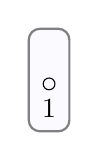
\begin{tikzpicture}
					%
					\node at (0,0.53) {}; 
					\node at (0,0) [node, label=below:$1$] (1) {};
					%
					\pgfBox
				\end{tikzpicture} 
			};
			\node[font=\scriptsize, above] at (k.north) {$K_0$};
			\node[below] at (k.south) {$\rho_0$};
			\node  [right=of k] (r) {
				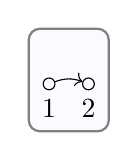
\begin{tikzpicture}
					\node at (0,0.53) {}; 
					\node at (0,0) [node, label=below:$1$] (1) {};
					\node at (.5,0) [node, label=below:$2$] (2) {};
					\draw[->] (1) to[out=20, in=160] (2);
					%
					\pgfBox
				\end{tikzpicture}
			};
			\node[font=\scriptsize, above] at (r.north) {$R_0$};
			\path (k) edge[->] node[trans, above] {} (l);
			\path (k) edge[->] node[trans, above] {} (r);    
		\end{tikzpicture}
		%  }
	%
	\hspace{1cm}
	%  \hfill
	%
	%  \subcaptionbox*{}{
		% RULE P1
		%
		\begin{tikzpicture}[node distance=2mm, font=\small]
			\node (l) {
				\begin{tikzpicture}
					%
					\node at (0,0.53) {}; 
					\node at (0,0) [node, label=below:$1$] (1) {} ;
					% 
					\pgfBox
				\end{tikzpicture} 
			};
			\node[font=\scriptsize, above] at (l.north) {$L_1$};
			\node [right=of l] (k) {
				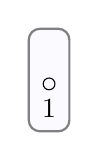
\begin{tikzpicture}
					%
					\node at (0,0.53) {}; 
					\node at (0,0) [node, label=below:$1$] (1) {};
					% 
					\pgfBox
				\end{tikzpicture} 
			};
			\node[font=\scriptsize, above] at (k.north) {$K_1$};
			\node[below] at (k.south) {$\rho_1$};
			\node  [right=of k] (r) {
				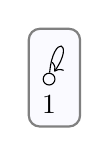
\begin{tikzpicture}
					\node at (0,0) [node, label=below:$1$] (1) {}
					edge [in=55, out=85, loop] ();
					%
					\pgfBox
				\end{tikzpicture}
			};
			\node[font=\scriptsize, above] at (r.north) {$R_1$};
			\path (k) edge[->] node[trans, above] {} (l);
			\path (k) edge[->] node[trans, above] {} (r);
		\end{tikzpicture}
		%  }
	% 
	\hspace{1cm}
	%\hfill
	%
	%    \subcaptionbox*{}{
		% RULE P2
		%
		\begin{tikzpicture}[node distance=2mm, font=\small]
			\node (l) {
				\begin{tikzpicture}
					%
					\node at (0,0.53) {}; 
					\node at (0,0) [node, label=below:$1$] (1) {} ;
					\node at (0.5,0) [node, label=below:$2$] (2) {} ;
					%
					\pgfBox
				\end{tikzpicture} 
			};
			\node[font=\scriptsize, above] at (l.north) {$L_2$};
			\node [right=of l] (k) {
				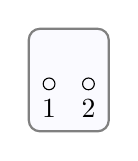
\begin{tikzpicture}
					%
					\node at (0,0.53) {}; 
					\node at (0,0) [node, label=below:$1$] (1) {} ;
					\node at (0.5,0) [node, label=below:$2$] (2) {} ;
					%
					\pgfBox
				\end{tikzpicture} 
			};
			\node[font=\scriptsize, above] at (k.north) {$K_2$};
			\node[below] at (k.south) {$\rho_2$};
			\node  [right=of k] (r) {
				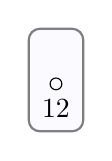
\begin{tikzpicture}
					\node at (0,0.53) {}; 
					\node at (0,0) [node, label=below:$12$] (12) {};
					%
					\pgfBox
				\end{tikzpicture}
			};
			\node[font=\scriptsize, above] at (r.north) {$R_2$};
			\path (k) edge[->] node[trans, above] {} (l);
			\path (k) edge[->] node[trans, above] {} (r);
		\end{tikzpicture}
	\end{center}
	
	We can also give an example of derivation as follows, where the colors are used to avoid ambiguity in the edges. Note that the numbers in $\rho_1$ were changed consistently to represent the vertical morphisms.
	
	\begin{center}
		\begin{tikzpicture}[node distance=2mm, font=\small, baseline=(current bounding box.center)]      
			\node (L0) at (0,2) {
				\begin{tikzpicture}
					% 
					\node at (0,0.53) {};
					\node at (0,0) [node, label=below:$1$] (1) {} ;
					% 
					\pgfBox
				\end{tikzpicture} 
			};
			\node [right=of L0] (K0) {
				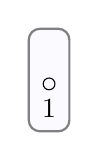
\begin{tikzpicture}
					% 
					\node at (0,0.53) {}; 
					\node at (0,0) [node, label=below:$1$] (1) {};
					% 
					\pgfBox
				\end{tikzpicture} 
			};
			\node [above] at (K0.north) {$\rho_0$};
			%     \node [above=of K1] {$\rho_0$};
			\node [right=of K0](R0) {
				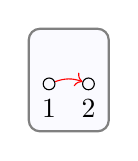
\begin{tikzpicture}
					\node at (0,0.53) {}; 
					\node at (0,0) [node, label=below:$1$] (1) {};
					\node at (.5,0) [node, label=below:$2$] (2) {};
					\draw[coloredge] (1) to[out=20, in=160] (2);
					% 
					\pgfBox
				\end{tikzpicture}
			};
			\path (K0) edge[->] node[trans, above] {} (L0);
			\path (K0) edge[->] node[trans, above] {} (R0);
			
			\node at (4,2) (L1) {
				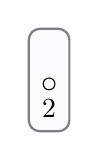
\begin{tikzpicture}
					% 
					\node at (0,0.53) {}; 
					\node at (0,0) [node, label=below:$2$] (2) {} ;
					% 
					\pgfBox
				\end{tikzpicture} 
			};
			\node [right=of L1] (K1) {
				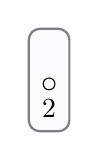
\begin{tikzpicture}
					% 
					\node at (0,0.53) {}; 
					\node at (0,0) [node, label=below:$2$] (2) {};
					% 
					\pgfBox
				\end{tikzpicture} 
			};
			%     \node [above=of K1] {$\rho_1$};
			\node [above] at (K1.north) {$\rho_1$};
			\node [right=of K1] (R1) {
				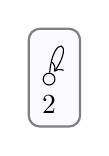
\begin{tikzpicture}
					\node at (0,0) [node, label=below:$2$] (2) {}
					edge [in=55, out=85, loop] ();        
					% 
					\pgfBox
				\end{tikzpicture}
			};
			\path (K1) edge[->] node[trans, above] {} (L1);
			\path (K1) edge[->] node[trans, above] {} (R1);
			
			\node at (8,2) (L2) {
				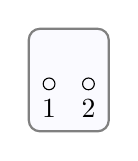
\begin{tikzpicture}
					% 
					\node at (0,0.53) {}; 
					\node at (0,0) [node, label=below:$1$] (1) {} ;
					\node at (0.5,0) [node, label=below:$2$] (2) {} ;
					% 
					\pgfBox
				\end{tikzpicture} 
			};
			\node [right=of L2] (K2) {
				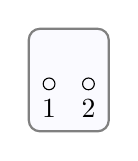
\begin{tikzpicture}
					% 
					\node at (0,0.53) {}; 
					\node at (0,0) [node, label=below:$1$] (1) {} ;
					\node at (0.5,0) [node, label=below:$2$] (2) {} ;
					% 
					\pgfBox
				\end{tikzpicture} 
			};
			%      \node [above=of K2] {$\rho_2$};
			\node [above] at (K2.north) {$\rho_2$};
			\node [right=of K2] (R2) {
				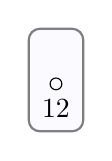
\begin{tikzpicture}
					\node at (0,0.53) {}; 
					\node at (0,0) [node, label=below:$12$] (12) {};
					% 
					\pgfBox
				\end{tikzpicture}
			};
			\path (K2) edge[->] node[trans, above] {} (L2);
			\path (K2) edge[->] node[trans, above] {} (R2);
			
			%%%%%% second row
			\node at (0,0) (G0) {
				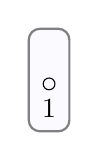
\begin{tikzpicture}
					% 
					\node at (0,0.53) {};
					\node at (0,0) [node, label=below:$1$] (1) {} ;
					% 
					\pgfBox
				\end{tikzpicture} 
			};
			\node [right=of G0] (D0) {
				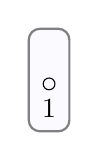
\begin{tikzpicture}
					% 
					\node at (0,0.53) {}; 
					\node at (0,0) [node, label=below:$1$] (1) {};
					% 
					\pgfBox
				\end{tikzpicture} 
			};
			\node at (3,0) (G1) {
				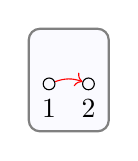
\begin{tikzpicture}
					% 
					\node at (0,0.53) {}; 
					\node at (0,0) [node, label=below:$1$] (1) {} ;
					\node at (0.5,0) [node, label=below:$2$] (2) {} ;
					\draw[coloredge] (1) to[out=20, in=160] (2);
					% 
					\pgfBox
				\end{tikzpicture} 
			};
			\path (D0) edge[->] node[trans, above] {} (G0);
			\path (D0) edge[->] node[trans, above] {} (G1);
			\path (L0) edge[->] node[trans, above] {} (G0);
			\path (K0) edge[->] node[trans, above] {} (D0);
			\path (R0) edge[->] node[trans, above] {} (G1);
			
			\node at (5,0) (D1) {
				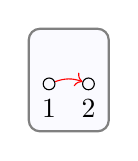
\begin{tikzpicture}
					% 
					\node at (0,0.53) {};
					\node at (0,0) [node, label=below:$1$] (1) {} ;
					\node at (0.5,0) [node, label=below:$2$] (2) {} ;
					\draw[coloredge] (1) to[out=20, in=160] (2);
					% 
					\pgfBox
				\end{tikzpicture} 
			};
			\node at (7,0) (G2) {
				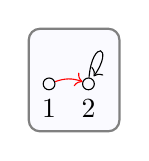
\begin{tikzpicture}
					% 
					\node at (0,0.53) {}; 
					\node at (0,0) [node, label=below:$1$] (1) {};
					\node at (0.5,0) [node, label=below:$2$] (2) {}
					edge [in=55, out=85, loop] (); 
					\draw[coloredge] (1) to[out=20, in=160] (2);
					% 
					\pgfBox
				\end{tikzpicture} 
			};
			
			\path (D1) edge[->] node[trans, above] {} (G1);
			\path (D1) edge[->] node[trans, above] {} (G2);
			\path (L1) edge[->] node[trans, above] {} (G1);
			\path (K1) edge[->] node[trans, above] {} (D1);
			\path (R1) edge[->] node[trans, above] {} (G2);
			
			\node at (9.46,0) (D2) {
				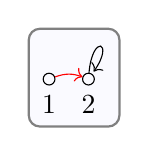
\begin{tikzpicture}
					% 
					\node at (0,0) [node, label=below:$1$] (1) {};
					\node at (0.5,0) [node, label=below:$2$] (2) {}
					edge [in=55, out=85, loop] ();
					\draw[coloredge] (1) to[out=20, in=160] (2);
					% 
					\pgfBox
				\end{tikzpicture} 
			};
			\node [right=of D2] (G3) {
				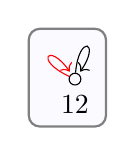
\begin{tikzpicture}
					% 
					\node at (0,0) [node, label=below:$12$] (12) {}
					edge [in=55, out=85, loop] ()
					edge [in=125, out=155, colorloop] ();
					% 
					\pgfBox
				\end{tikzpicture} 
			};
			\node[font=\scriptsize, below] at (G0.south) {$G_0$};
			\node[font=\scriptsize, below] at (D0.south) {$D_0$};      
			\node[font=\scriptsize, below] at (G1.south) {$G_1$};
			\node[font=\scriptsize, below] at (D1.south) {$D_1$};      
			\node[font=\scriptsize, below] at (G2.south) {$G_2$};
			\node[font=\scriptsize, below] at (D2.south) {$D_2$};      
			\node[font=\scriptsize, below] at (G3.south) {$G_3$};      
			\path (D2) edge[->] node[trans, above] {} (G2);
			\path (D2) edge[->] node[trans, above] {} (G3);
			\path (L2) edge[->] node[trans, above] {} (G2);
			\path (K2) edge[->] node[trans, above] {} (D2);
			\path (R2) edge[->] node[trans, above] {} (G3);
		\end{tikzpicture}
		%
	\end{center}
	
\end{example}

\begin{definition}
	The \emph{DPO-derivation category} $\dpo$ of a left-linear DPO-rewriting system $(\X, \R)$ is the category in which arrows between $G$ and $H$ are given by, possibly empty, derivations. Composition is concatenation of paths in $\gpo$ and identities are given by empty derivations.
\end{definition} 	
\begin{remark}
	More explicitly, given $\der{D}=\{\dder{D}\}_{i=0}^n$ between $G$ and $H$ and $\der{D}'=\{\dder{D}'_i\}_{i=0}^m$, their concatenation $\der{D}\cdot\der{D}'$ is the derivation $\{\dder{E}_i\}_{i=0}^{m+n+1}$ in which
	\[\dder{E}_i:=\begin{cases}
		\dder{D}_i & i \leq n\\
		\dder{D}'_{i-(n+1)} & n< i 
	\end{cases}\]	
	
	Notice, moreover that, $\der{D}\cdot \der{D'}$ is equal to $\der{D}'$ if $\der{D}$ is empty, while it coincides with $\der{D}$ if $\der{D}'$ has length zero.
\end{remark}

\Cref{exa:conc} allows us to compose derivations with isomorphisms.

\begin{definition} Let $(\X, \R)$ be a a left-linear DPO-rewriting system. Given a derivation $\der{D}=\{\dder{D}_{i}\}_{i=0}^n$ between $G$ and $H$ and isomorphisms $\phi\colon G'\to G$, $\psi\colon H\to H'$, the derivations  $\phi*\der{D}$ and $\der{D}*\psi$ are defined as
	\[\phi *\der{D} := \begin{cases}
		G' & \lgh(\der{D})=0\\ 
		\{\phi* \dder{D}_0\}\cdot \{\dder{D}_i\}_{i=1}^{n}  & \lgh(\der{D})\neq 0
	\end{cases} \qquad \der{D}*\psi := \begin{cases}
		H' & \lgh(\der{D})=0\\ 
		\{\dder{D}_i\}_{i=0}^{n-1} \cdot \{\dder{D}_n*\psi\} & \lgh(\der{D})\neq 0
	\end{cases}\] 
	
	Moreover, if $\lgh(\der{D})>0$,  we define the derivation $\phi *\der{D} * \psi$ as
	\[\phi *\der{D} * \psi = \{\phi* \dder{D}_0\}\cdot \{\dder{D}_i\}_{i=1}^{n-1} \cdot \{\dder{D}_n*\psi\}\] 
\end{definition}

\begin{remark}
	When $\der{D}$ consists only in the direct derivation $\dder{D}$, then $\phi*\der{D}*\psi$ is the derivation of length one whose unique element is $\phi*\dder{D}*\psi$.
\end{remark}

\subsection{Decorations and abstraction equivalence}
We are often interested in an object of $\X$ only up to isomorphism. It is therefore useful to consider a version of $\gpo$ in which vertices are classes of isomorphism of object of $\X$. In order to do so, some preliminary work is needed.

\begin{definition}\cite{mac2013categories}
	Let $\X$ be a category, we say that  $\X$ is \emph{skeletal} if, for every two objects $X$ and $Y$, the existence of an isomorphism $\phi\colon X\to Y$ entails $X=Y$. A \emph{skeleton} for a category $\X$ is a full subcategory $\ske$ which is skeletal and such that the inclusion functor $\ske\to \X$ is an equivalence. 
\end{definition}

\begin{remark}
	By definition the inclusion $\ske \to \X$ is an equivalence. In particular, for every objects $X$ of $\X$ there exists $\pi(X)$ in $\ske$ and an isomorphism $\phi_X\colon \pi(X) \to X$.
\end{remark}

\begin{proposition}\label{prop:ske}
	Every category $\X$ has a skeleton. 
\end{proposition}
\begin{proof}
	For every object $X\in \X$, pick a single representative $\pi(X)$ of its isomorphism class. Let $\ske$ be the full subcategory given by these objects. By definition $\ske$ is skeletal and the inclusion functor is full, faithful and essentially surjective.\qedhere 
\end{proof}
\begin{remark}
	The proof of \Cref{prop:ske} relies on the axiom of choice for classes.
\end{remark}
\begin{remark}
	It is possible to prove that every two skeleta of a given category $\X$ are isomorphic (not only equivalent). For the remaining of this paper we assume that a skeleton $\ske$ of $\X$ and a functor $\pi\colon \X\to \ske$ are chosen once and for all.
\end{remark}

\begin{definition}
	Let $(\X, \R)$ be a left-linear DPO-rewriting system, a \emph{decorated derivation} between two objects $G$ and $H$ is a triple $(\der{D}, \alpha, \omega)$, where $\der{D}$ is a derivation between $G$ and $H$, and $\alpha\colon \pi(G)\to G$ and $\omega\colon \pi(H)\to H$ are isomorphisms.
\end{definition}

\begin{notation}
	We will extend the use of the words length, source and target to decorated derivations in the obvious way, forgetting the decorations $\alpha$ and $\omega$.
\end{notation}

\begin{example}A decorated derivation $(\der{D}, \alpha, \omega)$ with $\der{D}$ empty is just a span
	\[\xymatrix{G & \pi(G) \ar[r]^-{\omega} \ar[l]_-{\alpha} & G}\]
	in which both $\omega$ and $\alpha$ are isomorphisms.
\end{example}

As we are interested in objects only up to isomorphism, so we are interested in (decorated) derivations only up to some notion of coherent isomorphism between them. This is done with the help of \Cref{rem:func}.

\begin{definition}Let $(\X, \R)$ be a left-linear DPO-rewriting system. An \emph{abstraction equivalence} between two derivations $\der{D}$ and $\der{D'}$ with the same length and such that $r(\der{D})=r(\der{D}')$ is a family of isomorphisms $\{\phi_X\}_{X\in \Deltamin(\der{D})}$ such that, for every $i\in [0, \lgh(\der{D})-1]$ the following diagram commutes
	\[\xymatrix@C=40pt{G'_i&D'_i \ar[r]^{g'_i} \ar@{>->}[l]_{f'_i}&G'_{i+1}\\  L_i \ar[u]^{m'_i} \ar[d]_{m_i}& K_i \ar[u]^{k'_i} \ar[d]_{k_i} \ar[r]^{r_i} \ar@{>->}[l]_{l_i} &R_i\ar[u]^{h'_i} \ar[d]_{h_i}\\G_i \ar@/_.45cm/[uu]_(.35){\phi_{G_i}}|\hole&D_i\ar@{>->}[l]^{f_i}\ar@/_.45cm/[uu]_(.35){\phi_{D_i}}|\hole \ar[r]_{g_i}&G_{i+1}\ar@/_.45cm/[uu]_{\phi_{H_i}}}\]
	
	If such an abstraction equivalence exists we will say that $\der{D}$ and $\der{D}'$ are \emph{abstraction equivalent} and we will use $\equiv^{abs}$ to denote the resulting relation-
	
Given two decorated derivations $(\der{D}, \alpha, \omega)$  and $(\der{D}', \alpha', \omega')$, with the same length $n$ and using the same rules, an abstraction equivalence $\{\phi_X\}_{X\in \Deltamin(\der{D})}$ is \emph{left consistent} if the left diagram below commutes, while it is \emph{right consistent} if the right one does so. A \emph{consistent} abstraction equivalence  is one which is both left and right consistent.
\[\xymatrix@C=15pt{&\pi(G_0) \ar[dr]^{\alpha'} \ar[dl]_{\alpha}&&& \pi(G_{n}) \ar[dr]^{\omega'} \ar[dl]_{\omega}\\ G_0 \ar[rr]_{\phi_{G_0}} && G'_0 &G_{n} \ar[rr]_{\phi_{G_{n}}} && G'_{n} } \]
	
We will say that $(\der{D}, \alpha, \omega)$  and $(\der{D}', \alpha', \omega')$ are \emph{left consistently}, respectively \emph{right consistently} or \emph{consistently}, abstraction equivalent, if there is a left consistent, respectively a right consistent or a consistent, abstraction equivalence between them. We will use $\equiv^{l}$, $\equiv^{r}$ and $\equiv^{a}$ to denote the resulting relations.
\end{definition}

\begin{proposition}\label{prop:equi}
The relations $\equiv^{abs}, \equiv^l, \equiv^r$ and $\equiv^a$ are equivalences.
\end{proposition}
\begin{proof}
	 
	 Let $\der{D}$ be a derivation, then $\{\id{X}\}_{X\in \Deltamin(\der{D})}$ is an abstraction equivalence between $\der{D}$ and itself. Moreover, starting with a decorated derivation $(\der{D}, \alpha, \omega)$, the same $\{\id{X}\}_{X\in \Deltamin(\der{D})}$  is also consistent, so that all the four relations are reflexive.
	 
	 For simmetry, let us suppose that $\{\phi_X\}_{X\in \Deltamin(\der{D})}$ is an abstraction equivalence between $\der{D}$ and $\der{D}'$, then $\{\phi^{-1}_X\}$ defines an abstraction equivalence  between $\der{D}'$ and $\der{D}$. Indeed, for every $i\in [0, \lgh(\der{D})-1]$ we have
	 \[\begin{split}
	 	m_i&=\id{G_i}\circ m_i\\&=\phi^{-1}_{G_i}\circ \phi_{G_i}\circ m_i\\&=\phi^{-1}_{G_i}\circ m'_i
	 \end{split} \qquad \begin{split}
 	k_i&=\id{D_i}\circ k_i\\&=\phi^{-1}_{D_i}\circ \phi_{D_i}\circ k_i\\&=\phi^{-1}_{D_i}\circ k'_i
	 \end{split}\qquad \begin{split}
 	h_i&=\id{G_{i+1}}\circ h_i\\&=\phi^{-1}_{G_{i+1}}\circ \phi_{G_{i+1}}\circ h_i\\&=\phi^{-1}_{G_{i+1}}\circ h'_i
	 \end{split} \]
	
	Starting with two decorated derivations $(\der{D}, \alpha, \omega)$ and $(\der{D}', \alpha', \omega')$, if $\{\phi_X\}_{X\in \Deltamin(\der{D})}$  is left, respectively right, consistent  then, putting $n$ as the length of $\der{D}$, we have:
	\[\begin{split}
		\alpha&=\id{G_0}\circ \alpha\\&=\phi^{-1}_{G_0}\circ \phi_{G_0}\circ \alpha\\&=\phi^{-1}_{G_0}\circ \alpha'
	\end{split}\qquad \begin{split}
		\omega&=\id{G_n}\circ \omega\\&=\phi^{-1}_{G_n}\circ \phi_{G_n}\circ \omega\\&=\phi^{-1}_{G_n}\circ \omega'
	\end{split}\]
	
	Finally, let $\{\phi_X\}_{X\in \Deltamin(\der{D})}$ and $\{\psi_X\}_{X\in \Deltamin(\der{D}')}$ be abstraction equivalence witnessing $\der{D} \equiv^{abs}\der{D}'$ and $\der{D}'\equiv^{abs}\der{D}''$. Then we can consider the family $\{\psi_X\circ \phi_X\}_{X\in \Deltamin(\der{D})}$  and check that, for every $i\in [0,\lgh(\der{D})]$ we have
	 \[\begin{split}
	\psi_{G_i}\circ \phi_{G_i}\circ m_i&= \psi_{G_i}\circ m'_i\\&=m''_i 
\end{split} \qquad \begin{split}
	\psi_{D_i}\circ \phi_{D_i}\circ k_i&= \psi_{D_i}\circ k'_i\\&=k''_i
\end{split}\qquad \begin{split}
\psi_{G_{i+1}}\circ \phi_{G_{i+1}}\circ h_i&= \psi_{G_{i+1}}\circ h'_i\\&=h''_i
\end{split} \]
	
	For decorations, if $\{\phi_X\}_{X\in \Deltamin(\der{D})}$ and $\{\psi_X\}_{X\in \Deltamin(\der{D}')}$ are left or right consistent we have
	 \[\begin{split}
		\psi_{G_0}\circ \phi_{G_0}\circ \alpha&= \psi_{G_0}\circ \alpha'\\&=\alpha'' 
	\end{split} \qquad \begin{split}
		\psi_{G_{\lgh(\der{D})}}\circ \phi_{G_{\lgh(\der{D})}}\circ \omega&= \psi_{G_{\lgh(\der{D})}}\circ \omega'\\&=\omega''
	\end{split}\]
	And we can conclude.
\end{proof}

\begin{notation}
	Since we are mainly interested into consistent abstraction equivalence, we will use  $[\der{D}, \alpha, \omega]_a$ to denote the equivalence class of  $(\der{D}, \alpha, \omega)$ with respect to $\equiv^a$.
	Such equivalence classes will be called  \emph{abstract decorated derivations}.  
\end{notation}

\begin{example}\label{rem:empty}
	Let $\{G\}$ and  $\{G'\}'$ be two empty derivations  An abstraction equivalence between $\{G\}$ and $\{G\}'$ is just an isomorphism $\phi\colon G\to G'$, so that $\pi(G)=\pi(G')$. If we are dealing with decorated derivations $(\{G\}, \alpha, \omega)$ and $(\{G'\}, \alpha, \omega)$,  left and right consistency of $\phi $ correspond to the commutativity of the diagrams below.
	\[\xymatrix@C=15pt{&\pi(G) \ar[dr]^{\alpha'} \ar[dl]_{\alpha}&&& \pi(G) \ar[dr]^{\omega'} \ar[dl]_{\omega}\\ G\ar[rr]_{\phi} && G' &G \ar[rr]_{\phi} && G' } \]
	
	In particular, this prove that two empty decorated derivations $(\{G\},\alpha, \omega) $ and $(\{G'\}',\alpha', \omega')$ are consistently abstraction equivalent if and only if
	\[	\alpha'\circ \alpha^{-1}=\omega'\circ \omega^{-1}\]
\end{example}

\begin{remark}\label{rem:res} \Cref{prop:unique} can be restated as saying that, given two direct derivations $\dder{D}$ and $\dder{D'}$ with the same match, there exists an abstract equivalence between them whose first component is the identity. 
\end{remark}

\begin{remark}\label{rem:absequi}
	Let $\der{D}$ be a derivation with source $G$ and target $H$. Let also $\phi\colon G'\to G$ and $\psi\colon H\to H'$ be two isomorphisms. Then for every $X\in \Deltamin(\der{D})$ we can define 
	\[\varphi_X:=\begin{cases}
		\phi^{-1} & X=G\\
		\id{X} & \text{otherwise}
	\end{cases} \qquad \varphi'_X:=\begin{cases}
		\psi & X=H\\
		\id{X} & \text{otherwise}
	\end{cases}\]
	It is immediate to see that the family $\{\varphi_X\}_{X\in \Deltamin(\der{D})}$ is an abstraction equivalence between $\der{D}$ and $\phi *\der{D}$, while $\{\varphi'_X\}_{X\in \Deltamin(\der{D})}$ is one between $\der{D}$ and $\der{D}*\psi$.  
	
	Taking in account the decorations, we also have that $\{\phi_X\}_{X\in \Deltamin(\der{D})}$ and  $\{\phi'_X\}_{X\in \Deltamin(\der{D})}$ witness, respectively, that 
	\[(\der{D}, \alpha, \omega) \equiv^a (\phi * \der{D}, \phi^{-1}\circ \alpha,   \varphi^{-1}_{H} \circ \omega) \qquad (\der{D}, \alpha, \omega) \equiv^a ( \der{D}*\psi, \varphi'_{G} \circ \alpha, \psi \circ \omega )\]

if $\der{D}$ is not empty, then the previous equations become
\[(\der{D}, \alpha, \omega) \equiv^a (\phi * \der{D}, \phi^{-1}\circ \alpha,   \omega) \qquad (\der{D}, \alpha, \omega) \equiv^a ( \der{D}*\psi, \alpha, \psi \circ \omega )\]

In particular, given an empty decorated derivation $(\{G\}, \alpha, \omega)$, we can apply what we have noticed to $\alpha \colon \pi(G)\to G$ and to $\omega^{-1}\colon G\to \pi(G) $ to get that 
\[(\{G\}, \alpha, \omega)\equiv^a (\{\pi(G)\}, \id{\pi(G)}, \alpha^{-1}\circ \omega) \qquad (\{G\}, \alpha, \omega)\equiv^a (\{\pi(G)\}, 	\omega^{-1}\circ \alpha, \id{\pi(G)})\]
\end{remark}


\begin{definition}\label{def:conc}
	Let $(\der{D}, \alpha, \omega)$ be a decorated derivation between $G$ and $H$ and $(\der{D}', \alpha', \omega')$ one between $H'$ and $K$. If $H$ and $H'$ are isomorphic, so that $\pi(H)=\pi(H')$, we define the  \emph{composite decorated derivation} putting
	\[(\der{D}, \alpha, \omega)\cdot (\der{D}', \alpha', \omega'):=\begin{cases}
		(\der{D}', \alpha'\circ \omega^{-1}\circ \alpha, \omega')	&\lgh(\der{D})=0 \\
		(\der{D}, \alpha, \omega \circ (\alpha')^{-1}\circ \omega')&\lgh(\der{D}')=0 \text{ and } \lgh(\der{D})\neq 0\\
		(\der{D}*\omega^{-1}\cdot \alpha'*\der{D'}, \alpha, \omega')	&\text{otherwise}
	\end{cases}\]
\end{definition}

\begin{remark}\label{rem:lgt}
	Let $(\der{D}, \alpha, \omega)$ and $(\der{D}', \alpha', \omega')$ two composable decorated derivations   such that $\lgh(\der{D})=n$ and $\lgh(\der{D}')=m$.	 Then $(\der{D}, \alpha, \omega)\cdot (\der{D}', \alpha', \omega')$ has length $n+m$.
\end{remark}

\begin{remark}\label{rem:id}
	Let  $(\{G\}, \alpha, \alpha)$ be a decoration of length $0$ with the same isomorphism as initial and final decoration. Then for every other derivations $(\der{D}, \beta, \omega)$ with source isomorphic to $G$, we have
	\[(\{G\}, \alpha, \alpha)\cdot (\der{D}, \beta, \omega) = (\der{D}, \beta, \omega)\]
	
	On the other hand, if  $(\der{E}, \gamma, \zeta)$  has a target isomorphic to $G$, we have
	\[(\der{E}, \gamma, \zeta)\cdot (\{G\}, \alpha, \alpha) = \begin{cases}
		(\{G\}, \alpha \circ \zeta^{-1}\circ \gamma, \alpha)	&\lgh(\der{E})=0 \\
		(\der{E}, \gamma, \zeta )& \lgh(\der{E})= 0
	\end{cases}\]
	
Now,  in the first case, we have that
\[\alpha \circ \zeta^{-1} \circ \gamma \circ \gamma ^{-1} = \alpha \circ \zeta^{-1}\]
therefore, by \Cref{rem:empty}, $(\der{E}, \gamma, \zeta)\cdot (\{G\}, \alpha, \alpha)\equiv^a  (\der{E}, \gamma, \zeta)$.
\end{remark}

\begin{remark}\label{ex:zero}
Let $(\{G\}, \alpha, \omega)$ and $(\{G'\}, \alpha', \omega')$ be two decorated derivations of length zero with $G$ and $G'$ isomorphic. Then we can always compose with another empty decorated derivations to get one from the other. In particular, using \Cref{rem:absequi} we have:
\begin{align*}
(\{G\}, \alpha, \omega)&\equiv^{a} (\pi(G), \id{\pi(G)}, \alpha^{-1}\circ \omega)\\&=(\{\pi(G)\}, (\alpha')^{-1}\circ \omega'\circ \omega'^{-1} \circ \alpha', \alpha^{-1}\circ \omega)\\&=(\{G'\}, \alpha', \omega')\cdot (\{\pi(G)\}, (\alpha')^{-1}\circ \omega', \alpha^{-1}\circ \omega)
\\(\{G\}, \alpha, \omega)&\equiv^{a} (\{\pi(G)\}, 	\omega^{-1}\circ \alpha, \id{\pi(G)})\\&=(\{\pi(G)\}, \omega^{-1}\circ \alpha, (\omega')^{-1}\circ\alpha'\circ (\alpha')^{-1} \circ \omega')\\&= (\{\pi(G)\}, \omega^{-1}\circ \alpha, (\omega')^{-1}\circ\alpha') \cdot (\{G'\}, \alpha', \omega')
\end{align*}
\end{remark}

We can generalize the previous remark to the following elementary, but useful, result about abstraction equivalence of composite decorated derivations. 
\begin{lemma}\label{rem:obv}
	Let  $(\der{D}_1, \alpha_1, \omega_1)$, $(\der{D}_2, \alpha_2, \omega_2)$, $(\der{D}'_1, \alpha'_1, \omega'_1)$ and $(\der{D}'_2, \alpha'_2, \omega'_2)$ be two pairs of composable derivations and define $(\der{E}, \xi, \theta)$ and $(\der{E}', \xi', \theta')$ as 
	\[(\der{E}, \xi, \theta):=(\der{D}_1, \alpha_1, \omega_1) \cdot (\der{D}_2, \alpha_2, \omega_2) \qquad (\der{E}', \xi', \theta'):=(\der{D}'_1, \alpha'_1, \omega'_1) \cdot (\der{D}'_2, \alpha'_2, \omega'_2)\]
	 If $\lgh(\der{D}_1)=\lgh(\der{D}'_1)$, $\lgh(\der{D}_2)=\lgh(\der{D}'_2)$ and $\der{E}\equiv^a \der{E}'$  then there exist empty derivations $(\{A\}, \gamma_1, \delta_1)$ and $(\{B\}, \gamma_2, \delta_2)$ such that
	 \[(\der{D}_1, \alpha_1, \omega_1) \equiv^a (\der{D}'_1, \alpha'_1, \omega'_1) \cdot  (\{A\}, \gamma_1, \delta_1) \qquad (\der{D}_2, \alpha_2, \omega_2) \equiv^a (\{B\}, \gamma_2, \delta_2)\cdot (\der{D}'_2, \alpha'_2, \omega'_2)  \]
\end{lemma}
\begin{proof} Let $\{\phi_X\}_{X\in \Deltamin(\der{E})}$ be an abstraction equivalent witnessing that $(\der{E}, \zeta, \theta)\equiv^{a}(\der{E}', \zeta', \theta')$.	We split the cases following \Cref{def:conc}.
	
	\smallskip \noindent $\lgh(\der{D}_1)=0$. In this case we have that
	\[(\der{E}, \zeta, \theta)=(\der{D}_2, \alpha_2\circ \omega^{-1}_1 \circ \alpha_1, \omega_2) \qquad (\der{E}', \zeta', \theta')=(\der{D}'_2, \alpha'_2\circ (\omega'_1)^{-1} \circ \alpha'_1, \omega'_2)\]
	By hypothesis $\der{D}_1$ and $\der{D}'_1$ are given by $\{G_{1,0}\}$ and $\{G'_{1,0}\}$. Moreover we know that $G_{1,0}$ is isomorphic to $G_{2,0}$ and  $G'_{1,0}$ to $G'_{2,0}$. Since $\phi_{G_{2,0}}$ is an isomorphism we conclude that $G_{1,0}$ and $G_{2,0}$ are isomorphic and we deduce the first half of the thesis from \Cref{ex:zero}. 
	
	For the second half, let us consider define $B$ as $\pi(G_{2,0})$ and
	\[\gamma_2:=\alpha^{-1}_1\circ \omega_1\qquad  \delta_2:=(\alpha'_1)^{-1}\circ \omega'_1  \]
	
	Hence we have
\[
(\{\pi(G_{2,0})\}, \alpha^{-1}_1\circ \omega_1,  (\alpha'_1)^{-1}\circ \omega'_1 )\cdot(\der{D}'_2, \alpha'_2, \omega'_2)  =(\der{D}_2, \alpha'_2\circ (\omega'_1)^{-1} \circ \alpha'_1\circ \alpha_1^{-1}\circ \omega_1, \omega'_2)\]
Now, by consistency of $\{\phi_{X}\}_{X\in \Deltamin(\der{D}_2)}$ we know that
\[\phi_{G_{2,0}}\circ \alpha_2\circ \omega^{-1}_1\circ \alpha_1=\alpha'_2\circ (\omega'_1)^{-1} \circ \alpha'_1\]
	therefore we also have the equality
	\[\phi_{G_{2,0}}\circ \alpha_2=\alpha'_2\circ (\omega'_1)^{-1} \circ \alpha'_1 \circ \alpha^{-1}_1\circ \omega_1 \]
	We conclude that $\{\phi_X\}_{X\in \der{D}_2}$ witnesses the thesis.
	
	\smallskip \noindent $\lgh(\der{D}_2)=0$ and $\lgh(\der{D}_1)\neq 0$. By definition we know that
	\[(\der{E}, \zeta, \theta)=(\der{D}_1, \alpha_1, \omega_1\circ \alpha_2^{-1}\circ \omega_2) \qquad (\der{E}', \zeta', \theta')=(\der{D}'_1, \alpha'_1, \omega'_1\circ (\alpha'_2)^{-1}\circ \omega'_2)\]
	
	Let $l$ be the length of $\der{D}_1$, and consider $(\{\pi(G'_{1, l})\}, (\omega'_2)^{-1}\circ \alpha'_2, \omega^{-1}_2\circ \alpha_2)$, so that
	\[ (\der{D}'_1, \alpha'_1, \omega'_1) \cdot  (\{\pi(G_{1, l})\}, (\omega'_2)^{-1}\circ \alpha'_2, \omega^{-1}_2\circ \alpha_2)= (\der{D}'_1, \alpha'_1, \omega'_1\circ (\alpha'_2)^{-1}\circ \omega'_2 \circ \omega^{-1}_2\circ \alpha_2)\]
	Now, let us consider the abstraction equivalence between  the decorated derivations $(\der{D}_1, \alpha_1, \omega_1)$ and  $(\der{D}'_1, \alpha'_1, \omega'_1) \cdot  (\{\pi(G_{1, l})\}, (\omega'_2)^{-1}\circ \alpha'_2, \omega^{-1}_2\circ \alpha_2)$ given by $\{\phi_X\}_{X\in \Deltamin(\der{D}_1)}$. On the one hand it is, by construction, left consistent.  On the other hand we know that 
	 
	\[\phi_{G_{1,l}}\circ \omega_1\circ \alpha_2^{-1}\circ \omega_2=\omega'_1\circ (\alpha'_2)^{-1}\circ \omega'_2 \]
	 
	 Composing on both sides with $\omega^{-1}_1\circ \alpha_2$ yields now the thesis.
	 
The second half of the thesis follows immediately from \Cref{ex:zero}.	
	
	\smallskip \noindent  $\lgh(\der{D}_1)$ and $\lgh(\der{D}_2)$ are both different from $0$. By \Cref{def:conc} in this case we have
	\[(\der{E}, \zeta, \theta)=(\der{D}_1*\omega^{-1}_1 \cdot \alpha_2*\der{D}_2, \alpha_1,\omega_2 ) \qquad (\der{E}', \zeta', \theta')=(\der{D}'_1*(\omega'_1)^{-1} \cdot \alpha'_2*\der{D}'_2, \alpha'_1,\omega'_2 )\]
	
	
	
\end{proof}

The next proposition justifies the use of decorations, guaranteeing that concatenation of abstract decorated derivations is well-defined.
\begin{lemma}\label{lem:conc}
	Given a decorated derivation $(\der{D}, \alpha, \omega)$  between $G$ and $H$ and  another one $(\der{E}, \beta, \xi)$ between $E$ and $K$ with $\pi(H)=\pi(E)$. If  $(\der{D}', \alpha', \omega')$ and $(\der{E}', \beta', \xi')$ are two other decorated derivations such that
	\[[\der{D}, \alpha, \omega]_a = [\der{D}', \alpha', \omega']_a \qquad [\der{D}, \beta, \xi]_a=[\der{E}', \beta', \xi']_a\]
	Then
	\[[(\der{D}, \alpha, \omega)\cdot (\der{E}, \beta, \xi)]_a=[(\der{D}', \alpha', \omega')\cdot (\der{E}', \beta', \xi')]_a\]
\end{lemma}

\begin{proof} Take two abstraction equivalences $\{\phi_X\}_{X\in \Deltamin(\der{D})}$ and $\{\varphi_X\}_{X\in \Deltamin(\der{D})}$ between $(\der{D}, \alpha, \omega)$ and $(\der{D}', \alpha', \omega')$ and between $(\der{E}, \beta, \xi)$ and $(\der{E}', \beta', \xi')$, respectively. To fix the notation, suppose that $(\der{D}', \alpha', \omega')$ goes from $G'$ to $H'$ and $(\der{E}', \beta', \xi')$ from $E'$ to $K'$. We have three cases.

	\smallskip \noindent  $\lgh(\der{D})=0$. Then, $\lgh(\der{D}')$ is $0$ too. By \Cref{def:conc} we have
		\begin{align*}
			(\der{D}, \alpha, \omega)\cdot (\der{E}, \beta, \xi)&=(\der{E}, \beta\circ \omega^{-1}\circ \alpha, \xi)\\
			(\der{D}', \alpha', \omega')\cdot (\der{E}', \beta', \xi')&=(\der{E}', \beta'\circ (\omega')^{-1}\circ \alpha', \xi')
		\end{align*}
		Now, notice that $G$ and $H$ must coincide. Moreover, by \Cref{rem:empty} we also know that $\pi(G)=\pi(G')$ too. The same \Cref{rem:empty} entails that the inner squares of the following diagram are commutative, so that the whole rectangle commutes too.
		\[\xymatrix@C=35pt{\pi(G) \ar[r]^{\alpha} \ar[d]_{\id{\pi(G)}}& G  \ar[d]_{\phi_G}\ar[r]^-{\omega^{-1}} & \pi(G) \ar[d]_{\id{\pi(G)}} \ar[r]^{\beta}& E \ar[d]^{\varphi_E}\\\pi(G') \ar[r]_{\alpha'}& G' \ar[r]_-{(\omega')^{-1}} & \pi(G') \ar[r]_{\beta'} & E'}\]
		
		We can  then conclude that $\{\varphi_X\}_{X\in \Deltamin(\der{D})}$ witnesses the fact that $(\der{E}, \beta\circ \omega^{-1}\circ \alpha, \xi)$ is abstraction equivalent to $(\der{E}', \beta'\circ (\omega')^{-1}\circ \alpha', \xi')$.
		
\smallskip \noindent  $\lgh(\der{D})\neq 0$ and $\lgh(\der{E})= 0$. As in the point above, we get that also $\der{E}'$  is an empty derivation, thus we have
		\begin{align*}
			(\der{D}, \alpha, \omega)\cdot (\der{E}, \beta, \xi)&=(\der{D},  \alpha, \omega \circ \beta^{-1}\circ \xi)\\
			(\der{D}', \alpha', \omega')\cdot (\der{E}', \beta', \xi')&=(\der{D}',  \alpha', \omega' \circ (\beta')^{-1}\circ \xi')
		\end{align*}
		In this case we have that $E=K$ and that $\pi(E)=\pi(E')$. From \Cref{rem:empty} we deduce that the diagram below commutes.
		\[\xymatrix@C=35pt{\pi(E) \ar[r]^{\xi} \ar[d]_{\id{\pi(E)}}& E  \ar[d]_{\varphi_E}\ar[r]^-{\beta^{-1}} & \pi(E) \ar[d]_{\id{\pi(E)}} \ar[r]^{\omega}& H \ar[d]^{\phi_H}\\\pi(E') \ar[r]_{\xi'}& E' \ar[r]_-{(\beta')^{-1}} & \pi(E') \ar[r]_{\omega'} & H'}\]
		The thesis now follows at once.
		
		\smallskip \noindent $\lgh(\der{D})\neq 0$ and $\lgh(\der{E})\neq 0$. In this case we have
		\begin{align*}
			(\der{D}, \alpha, \omega)\cdot (\der{E}, \beta, \xi)&=(\der{D}*\omega^{-1}\cdot \beta*\der{E}, \alpha, \xi)\\
			(\der{D}', \alpha', \omega')\cdot (\der{E}', \beta', \xi')&=(\der{D}'*(\omega')^{-1}\cdot \beta'*\der{E'}, \alpha', \xi')
		\end{align*}
		To fix the notation, suppose that $\der{D}$, $\der{D}'$, $\der{E}$ and $\der{E}'$ are given by
		\[\der{D}=\{\dder{D}_i\}_{i=0}^n \quad \der{D}'=\{\dder{D}'_i\}_{i=0}^n \quad \der{E}=\{\dder{E}_i\}_{i=0}^t \quad \der{E}'=\{\dder{E}'_i\}_{i=0}^t\]
		Moreover, noticing that the rule applied by $\dder{D}_i$ and the one applied in $\mathcal{E}_i$  must coincide with, respectively, the one applied in $\dder{D}'_i$ and the one applied $\dder{E}'_i$. We will also assume that $\dder{D}_i$, $\dder{D}'_i$, $\dder{E}_i$ and $\dder{E}'_i$ are given, respectively, by the following four diagrams. 
		\[\xymatrix{L_{\der{D},i} \ar[d]_{m_{\der{D}, i}}& K_{\der{D},i} \ar[d]_{k_{\der{D}, i}} \ar[r]^{r_{\der{D},i}} \ar@{>->}[l]_{l_{\der{D},i}} & R_{\der{D},i}\ar[d]^{h_{\der{D}, i}} &L_{\der{E},i} \ar[d]_{m_{\der{E}, i}}& K_{\der{E},i} \ar[d]_{k_{\der{E}, i}} \ar[r]^{r_{\der{E},i}} \ar@{>->}[l]_{l_{\der{E},i}} & R_{\der{E},i}\ar[d]^{h_{\der{E}, i}} \\G_i & D_i \ar[r]_{g_{\der{D},i}} \ar@{>->}[l]^{f_{\der{D},i}} & G_{i+1} & E_i & F_i\ar[r]_{g_{\der{E},i}} \ar@{>->}[l]^{f_{\der{E},i}}  & E_{i+1}}\]
		\[\xymatrix{L_{\der{D},i} \ar[d]_{m_{\der{D}', i}}& K_{\der{D},i} \ar[d]_{k_{\der{D}', i}} \ar[r]^{r_{\der{D},i}} \ar@{>->}[l]_{l_{\der{D},i}} & R_{\der{D},i}\ar[d]^{h_{\der{D}', i}} &L_{\der{E},i} \ar[d]_{m_{\der{E}', i}}& K_{\der{E},i} \ar[d]_{k_{\der{E}', i}} \ar[r]^{r_{\der{E},i}} \ar@{>->}[l]_{l_{\der{E},i}} & R_{\der{E},i}\ar[d]^{h_{\der{E}', i}} \\G'_i & D'_i \ar[r]_{g_{\der{D}',i}} \ar@{>->}[l]^{f_{\der{D}',i}} & G'_{i+1} & E'_i & F'_i\ar[r]_{g_{\der{E}',i}} \ar@{>->}[l]^{f_{\der{E}',i}}  & E'_{i+1}}\]
		
		Now, for every $X\in \Deltamin(\der{D}*\omega^{-1}\cdot \beta*\der{E})$ we can define
		\[\psi_X:=\begin{cases}
			\phi_X & X\in  \Deltamin(\der{D})\text{ and } X\neq H\\\varphi_X & X\in  \Deltamin(\der{E}) \text{ and } X\neq E\\\id{\pi(H)}& X=\pi(H)\end{cases}\]
		Notice that, since $\psi_G=\phi_G$ and $\psi_K=\varphi_K$ we have at once  the commutativity of the triangles
		\[\xymatrix@C=15pt{&\pi(G) \ar[dr]^{\alpha'} \ar[dl]_{\alpha}&&& \pi(K) \ar[dr]^{\xi'} \ar[dl]_{\xi}\\ G\ar[rr]_{\psi_G} && G' &K \ar[rr]_{\psi_K} && K' } \]
		
		
		To show that $\{\psi_X\}_{\Deltamin(\der{D}*\omega^{-1}\cdot \beta*\der{E})}$ is an abstraction equivalence, it is now enough to prove the commutativity of the diagrams below.
		\[\xymatrix@R=15pt@C=22pt{\pi(E')&&F'_0 \ar@{>->}[ll]_-{(\beta')^{-1}\circ f_{\der{E}',0}} \ar@{>->}@/^.2cm/[dll]^(.6){f_{\der{E}',0}} \ar[r]^{g_{\der{E}',0}}&E'_1 &G'_n&D'_n \ar[rr]^-{(\omega')^{-1}\circ g_{\der{D}',n}} \ar@/_.2cm/[drr]_(.6){g_{\der{D}',n}} \ar@{>->}[l]_{f_{\der{D}',n}}&&\pi(H')
			\\E' \ar[u]_{(\beta')^{-1}} &&&&&&&H' \ar[u]^{(\omega')^{-1}}
			\\  L_{\der{E}, 0} \ar[u]_{m_{\der{E}', 0}} \ar[d]^{m_{\der{E}, 0}}&& K_{\der{E}, 0} \ar[uu]_{k_{\der{E}', 0}} \ar[dd]^{k_{\der{E}, i}} \ar[r]^(.4){r_{\der{E},0}} \ar@{>->}[ll]_{l_{\der{E},0}} &R_{\der{E}, 0}\ar[uu]_{h_{\der{E}',0}} \ar[dd]^{h_{\der{E},0}} & L_{\der{D}, n} \ar[uu]^{m_{\der{D}',n}} \ar[dd]_{m_{\der{D},n}}& K_{\der{D}, n} \ar[uu]^{k_{\der{D}',n}} \ar[dd]_{k_{\der{D},n}} \ar[rr]^{r_{\der{D},n}} \ar@{>->}[l]_(.4){l_{\der{D},n}} &&R_{\der{D}, n}\ar[u]^{h_{\der{D}',n}} \ar[d]_{h_{\der{D},n}}
			\\E \ar[d]^{\beta^{-1}}&&&&&&&H \ar[d]_{\omega^{-1}}
			\\\pi(E) \ar@/^.7cm/[uuuu]^(.2){\id{\pi(E)}}&&F_0\ar@{>->}[ll]^{\beta^{-1}\circ f_{\der{E},0}}\ar@/^.7cm/[uuuu]^(.35){\varphi_{F_0}}|\hole \ar@{>->}@/_.2cm/[ull]_(.6){f_{\der{E},0}}\ar[r]_{g_{\der{E},0}}&E_1\ar@/^.7cm/[uuuu]^(.35){\varphi_{E_1}}|\hole&G_n \ar@/_.7cm/[uuuu]_(.35){\phi_{G_n}}|\hole&D_n\ar@{>->}[l]^{f_{\der{D},n}}\ar@/_.7cm/[uuuu]_(.35){\phi_{D_n}}|\hole \ar@/^.2cm/[urr]^(.6){g_{\der{D},n}}\ar[rr]_{\omega^{-1}\circ g_{\der{D},n}}&&\pi(H)\ar@/_.7cm/[uuuu]_(.2){\id{\pi(H)}}} \]
		
		To see this, in turn, it is enough to show that	the following squares are commutative.
		\[\xymatrix{R_{\der{D}, n} \ar[d]_{h_{\der{D}, n}}\ar[r]^{h_{\der{D}', n}} & H' \ar[d]_{(\omega')^{-1}} &L_{\der{E}, 0} \ar[d]^{m_{\der{E}, 0}}\ar[r]^{m_{\der{E}', 0}}& E' \ar[d]^{(\beta')^{-1}}\\H\ar[r]_{\omega^{-1}} &\pi(H)&E \ar[r]_{\beta^{-1}} & \pi(E)}\]
		\[\xymatrix{D_n \ar[rr]^{\phi_{D_n}} \ar[d]_{g_{\der{D}, n}}&&D'_n \ar[d]_{g_{\der{D}', n}}&F_0 \ar@{>->}[d]^{f_{\der{E}, 0}} \ar[rr]^{\varphi_{F_0}} && F_0' \ar@{>->}[d]^{f_{\der{E}', 0}}\\H \ar[r]_-{\omega^{-1}} &\pi(H)&H' \ar[l]^-{(\omega')^{-1}}  &E \ar[r]_-{\beta^{-1}} & \pi(E) & E' \ar[l]^-{(\beta')^{-1}}}\]
		
		For the first ones, we have
		\[
		\begin{split} 
			\omega^{-1} \circ h_{\der{D}, n}&=\id{\pi(H)}\circ \omega^{-1} \circ h_{\der{D}, n} \\&=(\omega')^{-1}\circ \phi_H \circ \omega \circ \omega^{-1} \circ h_{\der{D}, n}\\&=(\omega')^{-1}\circ \phi_H  \circ h_{\der{D}, n}\\&=(\omega')^{-1}  \circ h_{\der{D}', n}
		\end{split} \qquad  	\begin{split} 
			\beta^{-1} \circ m_{\der{E}, 0}&=\id{\pi(E)}\circ \beta^{-1} \circ m_{\der{E}, 0}\\&=(\beta')^{-1}\circ \varphi_{E} \circ \beta \circ \beta^{-1} \circ m_{\der{E}, 0}\\&=(\beta')^{-1}\circ \varphi_{E}  \circ m_{\der{E}, 0}\\&=(\beta')^{-1}  \circ m_{\der{E}', 0}
		\end{split}  \]
		
		Similarly, the commutativity of the second row of diagrams can be deduced from
		\[\begin{split}
			\omega^{-1} \circ g_{\der{D}, n}&=\id{\pi(H)}\circ \omega^{-1} \circ g_{\der{D}, n}\\&=(\omega')^{-1}\circ \phi_H \circ \omega\circ \omega^{-1} \circ g_{\der{D}, n}\\&=(\omega')^{-1}\circ \phi_H  \circ g_{\der{D}, n}\\&= (\omega')^{-1} \circ g_{\der{D}', n}\circ \phi_{D_n}
		\end{split}\qquad \begin{split}\beta^{-1} \circ f_{\der{E}, 0}&=\id{\pi(E)}\circ \beta^{-1} \circ f_{\der{E}, 0}\\&=(\beta')^{-1}\circ \varphi_E \circ \beta\circ \beta^{-1} \circ f_{\der{E}, 0}\\&=(\beta')^{-1}\circ \varphi_E  \circ f_{\der{E}, 0}\\&= (\beta')^{-1} \circ f_{\der{E}', n}\circ \varphi_{F_0}
		\end{split}\]
		
		The thesis now follows.	
\end{proof}

We are now ready to prove that the operatione defined by \Cref{def:conc} is associative up to decorated abstraction equivalence.

\begin{lemma}[Associativity Lemma]\label{lem:ass}  
Let $(\der{D}_1, \alpha_1, \omega_1)$ be a decorated derivation between $G$ and $H$, $(\der{D}_2, \alpha_2, \omega_2)$, one between $H$ and $K$ and $(\der{D}_3, \alpha_3, \omega_3)$ one between $K$ and $T$ in a left-linear DPO rewriting system. Then
\[((\der{D}_1, \alpha_1, \omega_1)\cdot (\der{D}_2, \alpha_2, \omega_2)) \cdot (\der{D}_3, \alpha_3, \omega_3) \equiv^a (\der{D}_1, \alpha_1, \omega_1)\cdot ( (\der{D}_2, \alpha_2, \omega_2)\cdot (\der{D}_3, \alpha_3, \omega_3))\]
\end{lemma}
\begin{proof} We have seven cases.
	
\smallskip \noindent  $\der{D}_1$, $\der{D}_2$ are both empty.
In this case computing we get:
\begin{align*}
	((\der{D}_1, \alpha_1, \omega_1)\cdot (\der{D}_2, \alpha_2, \omega_2)) \cdot (\der{D}_3, \alpha_3, \omega_3)&=(\der{D}_2, \alpha_2\circ \omega^{-1}_1 \circ \alpha_1, \omega_2)\cdot (\der{D}_3, \alpha_3,\omega_3)\\&=(\der{D}_3,\alpha_3\circ\omega^{-1}_2\circ \alpha_2\circ \omega^{-1}_1\circ \alpha_1 ,\omega_3)\\&=(\der{D}_1, \alpha_1, \omega_1) \cdot (\der{D}_3, \alpha_3\circ \omega^{-1}_2 \circ \alpha_2,\omega_3)\\&=(\der{D}_1, \alpha_1, \omega_1) \cdot ((\der{D}_2, \alpha_2, \omega_2)\cdot (\der{D}_3, \alpha_3, \omega_3))
\end{align*}


\smallskip \noindent $\der{D}_1$ and $\der{D}_3$ are empty while $\der{D}_2$ is not. Apply \Cref{def:conc} we get
\begin{align*}
((\der{D}_1, \alpha_1, \omega_1)\cdot (\der{D}_2, \alpha_2, \omega_2)) \cdot (\der{D}_3, \alpha_3, \omega_3)&=(\der{D}_2, \alpha_2\circ \omega^{-1}_1 \circ \alpha_1, \omega_2)\cdot (\der{D}_3, \alpha_3,\omega_3)\\&=(\der{D}_2, \alpha_2\circ \omega^{-1}_1 \circ \alpha_1, \omega_2\circ \alpha^{-1}_3 \circ \omega_3)\\&=(\der{D}_1, \alpha_1, \omega_1 )\cdot  (\der{D}_2, \alpha_2,\omega_2\circ \alpha^{-1}_3 \circ  \omega_3)\\&= (\der{D}_1, \alpha_1, \omega_1 )\cdot((\der{D}_2, \alpha_2, \omega_2)\cdot (\der{D}_3, \alpha_3, \omega_3) )
\end{align*}


\smallskip \noindent  $\der{D}_1$ is empty, $\der{D}_2$ and $\der{D}_3$ are not. As above we can compute to get
\begin{align*}
((\der{D}_1, \alpha_1, \omega_1)\cdot (\der{D}_2, \alpha_2, \omega_2)) \cdot (\der{D}_3, \alpha_3, \omega_3)&=(\der{D}_2, \alpha_2\circ \omega^{-1}_1 \circ \alpha_1, \omega_2)\cdot (\der{D}_3, \alpha_3, \omega_3)\\&=(\der{D}_2*\omega^{-1}_2\cdot \alpha_3*\der{D}_3, \alpha_2\circ \omega^{-1}_1 \circ \alpha_1, \omega_3 )\\&=(\der{D}_1, \alpha_1, \omega_1) \cdot (\der{D}_2*\omega^{-1}_2\cdot \alpha_3*\der{D}_3, \alpha_2, \omega_3 )\\&=(\der{D}_1, \alpha_1, \omega_1) \cdot ((\der{D}_2, \alpha_2, \omega_2) \cdot (\der{D}_3, \alpha_3, \omega_3)  )
\end{align*}

\smallskip \noindent $\der{D}_1$ is non-empty while $\der{D}_2$ and $\der{D}_3$ have length $0$. Therefore:
\begin{align*}
	((\der{D}_1, \alpha_1, \omega_1)\cdot (\der{D}_2, \alpha_2, \omega_2)) \cdot (\der{D}_3, \alpha_3, \omega_3)&=(\der{D}_1, \alpha_1, \omega_1\circ \alpha^{-1}_2\circ \omega_2)\cdot (\der{D}_3, \alpha_3, \omega_3)\\&=(\der{D}_1, \alpha_1, \omega_1\circ \alpha^{-1}_2\circ \omega_2\circ \alpha^{-1}_3 \circ \omega_3 )\\&=(\der{D}_1, \alpha_1, \omega_1) \cdot (\der{D}_3, \alpha_3\circ \omega^{-1}_2\circ \alpha_2, \omega_3)\\&=(\der{D}_1, \alpha_1, \omega_1) \cdot ((\der{D}_2, \alpha_2, \omega_2) \cdot (\der{D}_3, \alpha_3, \omega_3)  )
\end{align*}


\smallskip \noindent $\der{D}_1$ and $\der{D}_3$ are non-empty while $\der{D}_2$ is. As above we have 

\begin{align*}
	((\der{D}_1, \alpha_1, \omega_1)\cdot (\der{D}_2, \alpha_2, \omega_2)) \cdot (\der{D}_3, \alpha_3, \omega_3)&=(\der{D}_1, \alpha_1, \omega_1\circ \alpha^{-1}_2\circ \omega_2)\cdot (\der{D}_3, \alpha_3, \omega_3)\\&=(\der{D}_1*(\omega^{-1}_2\circ \alpha_2\circ \omega^{-1}_1)\cdot \alpha_3*\der{D}_3, \alpha_1, \omega_3 )\\(\der{D}_1, \alpha_1, \omega_1) \cdot ((\der{D}_2, \alpha_2, \omega_2) \cdot (\der{D}_3, \alpha_3, \omega_3)  )&=(\der{D}_1, \alpha_1, \omega_1) \cdot (\der{D}_3, \alpha_3\circ \omega^{-1}_2\circ \alpha_2, \omega_3)\\&=(\der{D}_1*\omega^{-1}_1\cdot (\alpha_3\circ \omega^{-1}_2 \circ \alpha_2)*\der{D}_3, \alpha_1, \omega_3)
\end{align*}

Let $n$ be the length of $\der{D}_1$, so that $\pi(G_{1,n})=\pi(G_{3,0})$. We can notice that the following two diagrams commute.
	\[\xymatrix@C=55pt{G_{1, n-1}&D_{1,n-1} \ar[r]^{g_{1,n}} \ar@{>->}[l]_{f_{1,n}}&G_{1,n}  \ar[r]^{\omega^{-1}_1}& \pi(G_{1,n})\\  L_{1,n-1} \ar[u]_{m_{1,n-1}} \ar[d]^{m_{1, n-1}}& K_{1, n-1} \ar[u]^{k_{1,n-1}} \ar[d]_{k_{1,n-1}} \ar[rr]^{r_{1, n-1}} \ar@{>->}[l]_{l_{1,n-1}} &&R_{1, n-1}\ar[u]^{\omega^{-1}_1\circ h_{1,n-1}} \ar[d]_{\omega^{-1}_2\circ \alpha_2\circ \omega^{-1}_1\circ h_{1, n-1}}\\G_{1, n-1} \ar@/^.80cm/[uu]^{\id{G_{1, n-1}}}&D_{1, n-1}\ar@{>->}[l]^{f_{1, n-1}}\ar@/_.80cm/[uu]_(.35){\id{D_{1, n-1}}}|\hole \ar[r]_{g_{1, n-1}}&G_{1, n}\ar[r]_-{\omega^{-1}_2\circ \alpha_2\circ \omega^{-1}_1}& \pi(G_{1, n})\ar@/_.80cm/[uu]_{\alpha^{-1}_2\circ \omega_2}}\]
		\[\xymatrix@C=55pt{\pi(G_{3, 0}) & G_{3,0}  \ar[l]_-{\alpha_3\circ \omega^{-1}_2\circ \alpha_2}&D_{3,0} \ar[r]^{g_{3,0}} \ar@{>->}[l]_{f_{3,0}}&G_{3,1}  \\  L_{3,0} \ar[u]_{\alpha_3\circ \omega^{-1}_2\circ \alpha_2\circ m_{3,0}} \ar[d]^{\alpha_3\circ  m_{3, 0}}& & K_{3, 0} \ar[u]^{k_{3,0}} \ar[d]_{k_{3,0}} \ar[r]^{r_{3, 0}} \ar@{>->}[ll]_{l_{3,0}} &R_{3, 0}\ar[u]^{ h_{3,0}} \ar[d]_{ h_{3, 0}}\\\pi(G_{3, 0})  \ar@/^.80cm/[uu]^{\alpha^{-1}_2\circ \omega_2}&G_{3,0} \ar[l]^{\alpha_3}&D_{3, 0}\ar@{>->}[l]^{f_{3, 0}}\ar@/_.80cm/[uu]_(.35){\id{D_{3, 0}}}|\hole \ar[r]_{g_{3, 0}}&G_{3, 1}\ar@/_.80cm/[uu]_{\id{G_{3,1}}}}\]
	
Thus the family $\{\phi_{X}\}_{X\in \Deltamin(\der{D}_1*(\omega^{-1}_2\circ \alpha_2\circ \omega^{-1}_1)\cdot \alpha_3*\der{D}_3)}$ defined as
\[\phi_X:=\begin{cases}
	\id{X} & X\neq \pi(G_{1,n})\\
	\alpha^{-1}_2 \circ \omega_2 & X= \pi(G_{1,n})
\end{cases}\]
is a consistent abstraction equivalence witnessing our thesis.



\smallskip \noindent  $\der{D}_1$, $\der{D}_2$ and $\der{D}_3$ are all non-empty. For this case we rely to the fact that concatenation of derivations, being simply concatenation of paths in a graph, is associative. Indeed we have
\begin{align*}
	((\der{D}_1, \alpha_1, \omega_1)\cdot (\der{D}_2, \alpha_2, \omega_2)) \cdot (\der{D}_3, \alpha_3, \omega_3)&=(\der{D}_1*\omega^{-1}_1\cdot \alpha_2*\der{D}_2, \alpha_1, \omega_2)\cdot (\der{D}_3, \alpha_3, \omega_3)\\&=((\der{D}_1*\omega^{-1}_1\cdot \alpha_2*\der{D}_2)*\omega^{-1}_2\cdot \alpha_3*\der{D}_3, \alpha_1, \omega_3 )\\&=(\der{D}_1*\omega^{-1}_1\cdot (\alpha_2*\der{D}_2*\omega^{-1}_2)\cdot \alpha_3*\der{D}_3, \alpha_1, \omega_3 )\\&=(\der{D}_1*\omega^{-1}_1\cdot \alpha_2*(\der{D}_2*\omega^{-1}_2 \cdot \alpha_3*\der{D}_3), \alpha_1, \omega_3)\\&=(\der{D}_1, \alpha_1, \omega_1) \cdot (\der{D}_2*\omega^{-1}_2 \cdot \alpha_3*\der{D}_3, \alpha_2, \omega_3)\\&=
	(\der{D}_1, \alpha_1, \omega_1) \cdot ((\der{D}_2, \alpha_2, \omega_2) \cdot (\der{D}_3, \alpha_3, \omega_3))
\end{align*}
And the thesis now follows.
\end{proof}

Given \Cref{rem:id}  and \Cref{lem:ass}, we are now ready to give the following definition.

\begin{definition}
	Let $(\X, \R)$ be a left-linear DPO-rewrityng system, with $\X$ an $\mathcal{M}$-adhesive category. The  category $\dpi$ is defined as follows:
	\begin{itemize}
		\item objects are isomorphism classes of objects of $\X$;
		\item an arrow $[G]\to [H]$ is an equivalence class $[\der{D}, \alpha, \omega]_a$ of a decorated derivation between $G'$ and $H'$ for some $G'$ and $H'$ such that $\pi(G')=G$ and $\pi(H')=H$;
		\item composition is concatenation of abstract decorated derivations;
		\item the identity on $[G]$ is $[\{G\}, \alpha, \alpha]_a$, where $\alpha$ is any isomorphism $\pi(G)\to G$.	\end{itemize}
\end{definition}


In the next proposition we fully characterize the isomorphism in $\dpi$.

\begin{proposition} Let $(\X, \R)$ be a left-linear DPO rewriting system, then the isomorphisms in $\dpi$ are exactly the classes of empty decorated derivations.
\end{proposition}
\begin{proof}
	Let $[\der{D}, \alpha, \omega]_a$ be an isomorphism, thus there exists $(\der{E}, \beta, \gamma)$ such that $(\der{D}, \alpha, \omega)\cdot (\der{E}, \beta, \gamma)\equiv^a(\{G_{\der{D}, 0}\}, \alpha, \alpha)$. Since the latter has length $0$, \Cref{rem:lgt} entails that $\der{D}$ is empty too.
	
	Vice versa, if $(\{G\}, \alpha, \omega)$ is a derivation of length $0$, then 
	\begin{align*}
	(\{G\}, \alpha, \omega) \cdot (\{G\}, \omega, \alpha)&=(\{G\}, \omega\circ \omega^{-1} \circ \alpha, \alpha )\\&=(\{G\}, \alpha, \alpha)\\
	(\{G\}, \omega, \alpha) \cdot (\{G\}, \alpha, \omega)&=(\{G\}, \alpha\circ \alpha^{-1} \circ \omega, \omega )\\&=(\{G\}, \omega, \omega)
	\end{align*}
	showing that  $[\{G\}, \alpha, \omega]_a$ is an isomorphism.
\end{proof}

\subsection{Colimits of derivations}\label{subsec:col}
Given a DPO-rewriting system $(\X, \R)$,  we have already noted in \Cref{rem:func} that a derivation $\der{D}$  determines a diagram $\Delta(\der{D})$ in $\X$. We can then wonder if such a diagram has a colimit. Clearly if $\der{D}$ is the empty derivation $G$ then a colimit for $\Delta(\der{D})$ is simply the object $G$. More generally, we have the following result.

\begin{lemma}\label{lem:colim}
	Let $\X$ be an $\mathcal{M}$-adhesive category and $(\X, \R)$ a left-linear DPO-rewriting system over it. The following properties hold true:
	\begin{enumerate}
		\item  if $\der{D}$ is a derivation from $G$ to $H$, then the diagram $\Delta(\der{D})$ has a colimit $(\tpro{D}, \{\iota_X\}_{X\in \Delta(\der{D})})$ such that $\iota_H$ belongs to $\mathcal{M}$.
		\item if $\der{D}$ is the concatenation $\der{D}_1\cdot \der{D}_2$ of two derivations $\der{D}_1=\{\dder{D}_{1,i}\}_{i=0}^{n_1}$ between $G$ and $H$ and $\der{D}_2=\{\dder{D}_{2,j}\}_{j=0}^{n_2}$ between $H$ and $T$,  then the colimiting cocone $(\tpro{D}, \{\iota_X\}_{X\in \Delta(\der{D})})$ exists too and there is a pushout square
		\[\xymatrix{H\ar[r]^-{\iota_{2, H}} \ar@{>->}[d]_-{\iota_{1, H}} & \tproi{D}{2} \ar[d]^{p_2}\\  \tproi{D}{1} \ar[r]_{p_1}& \tpro{D}}\]
		where $(\tproi{D}{1}, \{\iota_{1, X}\}_{X\in \Delta(\der{D}_1)})$ and $(\tproi{D}{2}, \{\iota_{2, X}\}_{X\in \Delta(\der{D}_2)})$ are the colimiting cocone for $\Delta(\der{D}_1)$ and $\Delta(\der{D}_2)$, respectively.
	\end{enumerate}
\end{lemma}
\begin{remark}\label{rem:cof}
Let $I:\Deltamin(\dder{D})\to \Delta(\dder{D})$ be the inclusion functor. It is immediate to see that such functor is \emph{final} \cite{mac2013categories}. This means that for every functor $F\colon \Delta(\dder{D})\to \Y$ we have:
\begin{enumerate}
	\item if  $(C, \{c_X\}_{X\in \Deltamin(\dder{D})})$ is colimiting for $F\circ I$, then there exists a colimiting cocone $(D, \{d_X\}_{X\in \Delta(\dder{D})})$ for $F$;
	\item $(C, \{c_X\}_{X\in \Deltamin(\dder{D})})$ and $(D, \{d_X\}_{X\in \Delta(\dder{D})})$ are colimiting for, respectively, $F\circ I$ and $F$, then the canonical arrow $\phi\colon C\to D$ induced by $(D, \{d_X\}_{X\in \Deltamin(\dder{D})})$ is an isomorphism.
\end{enumerate}
\end{remark}

\begin{proof}\begin{enumerate}
		\item Let us proceed by induction on the length of $\der{D}$.

	
	\smallskip \noindent $\lgh(\dder{D})=0$. then the $\tpro{\dder{D}}$ is simply $(G, \{\id{G}\})$ and $\id{G}\in \mathcal{M}$.
	
	\smallskip \noindent$\lgh(\dder{D})=1$. Suppose that $\dder{D}$ has as its single component the derivation
			\[\xymatrix{L \ar[d]_{m}& K \ar[d]^{k}\ar@{>->}[l]_{l} \ar[r]^{r} & R \ar[d]^{h} \\G& \ar@{>->}[l]^{f} D \ar[r]_{g}& H  \\}\]
			The arrow $f$ is  the pushout of $l$ and so it is in in $\mathcal{M}$. We can thus consider the following $\mathcal{M}$-pushout square.
			\[\xymatrix{D \ar@{>->}[d]_{f} \ar[r]^{g} & H \ar@{>->}[d]^{p} \\G \ar[r]_{q}& P }\]
			Since $p\in \mathcal{M}$, the thesis follows immediately from \Cref{rem:cof}. 
	
	\smallskip \noindent$\lgh(\dder{D})\geq 2$. Let $\der{D}$ be $\{\dder{D}_i\}_{i=0}^n$ with $n\geq 1$. Let also $\der{D}'$ be $\{\dder{D}_i\}^{n-1}_{i=0}$ and $\rho_n=(l_n, r_n)$ be the rule applied in $\dder{D}_n$. The arrow $f_n\colon D_n\to G_n$, being a pushout of $l_n$ is an element $\mathcal{M}$. By inductive hypothesis, $\iota_{G_{n}}\colon G_{n}\to \lpro \der{D}'\rpro$ is in $\mathcal{M}$ too, thus, we can consider the diagram below, having a pushout as its lower half.
			\[\xymatrix{L_n \ar[d]_{m_{n}}& K_{n} \ar[d]^{k_{n}}\ar@{>->}[l]_{l_{n}} \ar[r]^{r_{n}} & R_{n} \ar[d]^{h_n} \\G_{n} \ar@{>->}[d]_{\iota'_{G_{n}}}& \ar@{>->}[l]^{f_n} D_n \ar[r]_{g_n}& H  \ar@{>->}[d]^{q}\\ \lpro \der{D}' \ar[rr]_{p}\rpro && P}\] 
			Notice that, as in the point above, the arrow $q\colon H\to P$ is the pushout of an element in $\mathcal{M}$, therefore it is enough to show that the diagram so constructed provides a colimiting cocone for $\Delta(\der{D})$.
			
			Let $(C, \{c_X\}_{X\in \Delta(\der{D})})$ be a cocone. Since $\Delta(\der{D}')$ is a subdiagram of $\Delta(\der{D})$, we get another cocone $(C, \{c_X\}_{X\in \Delta(\der{D}')})$ which induces an arrow $c'\colon \lpro \der{D}' \rpro \to C$ such that
			\begin{align*}
				c'\circ \iota_{G_n} \circ f_n &=c_{G_n} \circ f_n\\&= c_{D_n}\\&= c_{H}\circ g_n
			\end{align*}
			Therefore the arrows $c'$ and $c_H$ induce a morphism $c\colon P\to C$ and the thesis now follows at once.
		
		\item  As a first step, notice that $(\tpro{D}, \{\iota_X\}_{X\in \Delta(\der{D}_1)})$ and $(\tpro{D}, \{\iota_X\}_{X\in \Delta(\der{D}_2)})$ are cocone on, respectively, $\Delta(\der{D}_1)$ and $\Delta(\der{D}_2)$. Hence, there exist two arrows $p_1\colon \tproi{D}{1}\to \tpro{D}$, $p_2\colon \tproi{D}{2}\to \tpro{D}$ such that, for every $X\in  \Delta(\der{D}_1)$ and $Y\in  \Delta(\der{D}_2)$
		\[p_1\circ \iota_{1, X} = \iota_X \qquad p_2\circ \iota_{2, Y}=\iota_{2,Y}\]
		In particular, this entails the commutativity of the square
				\[\xymatrix{H \ar[dr]^{\iota_H} \ar[r]^-{\iota_{2, H}} \ar@{>->}[d]_-{\iota_{1, H}} & \tproi{D}{2} \ar[d]^{p_2}\\  \tproi{D}{1} \ar[r]_{p_1}& \tpro{D}}\]
		
	Let us now show that the square above is a pushout. Take two arrows $a\colon \tproi{D}{1}\to C$, $b\colon \tproi{D}{2}\to C$ such that $a\circ \iota_{1, H}=b\circ \iota_{2, H}$. We can use the previous equality to define a cocone $(C, \{c_X\}_{X\in \Delta(\der{D})})$ putting:
	\[c_X:=\begin{cases}
		a\circ \iota_{1, X} & X\in \Delta(\der{D}_1)\\
		b\circ \iota_{2, X} & X\in \Delta(\der{D}_2)
	\end{cases}\]
From this, we can deduce at once the existence of a unique $c\colon \tpro{D}\to C$ such that $c\circ \iota_X = c_X$. By construction, for every $X\in  \Delta(\der{D}_1)$ and $Y\in  \Delta(\der{D}_2)$ we have
\[\begin{split}
	c\circ p_1 \circ \iota_{1,X}&=c\circ \iota_{X}\\&=c_X \\&=a\circ \iota_{1,X}\\&=a\circ p_1\circ \iota_{1,X}
\end{split}\qquad \begin{split}
	c\circ p_2 \circ \iota_{2,Y}&=c\circ \iota_{Y}\\&=c_Y \\&=b\circ \iota_{2,Y}\\&=b\circ p_2\circ \iota_{2,Y}
\end{split}\]
Therefore we get that $c\circ p_1=a$ and $c\circ p_2 = b$.

	For uniqueness, suppose that $c'\colon \tpro{D}\to C$ is such that $c'\circ p_1=a$ and  $c'\circ p_2 = b$. Then, for every $X\in \Delta(\der{D})$ we have
\begin{align*}
	c'\circ \iota_X &= \begin{cases}
	c'\circ p_1\circ \iota_{1, X} & X\in \Delta(\der{D}_1)\\
	c'\circ p_2\circ \iota_{2, X} & X\in \Delta(\der{D}_2)
	\end{cases}\\&=\begin{cases}
a\circ \iota_{1, X} & X\in \Delta(\der{D}_1)\\
b\circ \iota_{2, X} & X\in \Delta(\der{D}_2)
	\end{cases}\\&=c_X\\&=c\circ \iota_X
\end{align*}
showing that $c'=c$ as wanted.	 \qedhere 
	\end{enumerate}
\end{proof}

\begin{corollary}\label{cor:colim}
Let $\der{D}=\{\dder{D}_i\}_{i=0}^n$ a derivation of length $n+1$ and fix an index $j\in[0,n]$. Define
\[\der{D}^j_1:=\{\dder{D}_i\}_{i=0}^{j-1} \qquad  \der{D}^j_2=\{\dder{D}_j\} \qquad \der{D}^j_3:=\{\dder{D}_i\}_{i=j+1}^n\]
with the convention that $\der{D}^0_1$ and $\der{D}^n_3$ are the empty derivation on, respectively, $G_0$ and $G_n$. Then the square below is a pushout and a pullback
\[\xymatrix@C=30pt{D_{j} \ar[ddrr]^{\iota_{D_j}} \ar[r]^{g_j}\ar@{>->}[d]_{f_j}& G_{j+1} \ar[ddr]^{\iota_{G_{j+1}}} \ar[r]^-{\iota_{3, G_{j+1}}} & \lpro \der{D}^j_3\rpro \ar[dd]^{p_2} \\ G_j\ar[drr]_{\iota_{G_{j}}} \ar@{>->}[d]_{\iota_{1,G_j}}\\ \lpro \der{D}^j_1 \rpro \ar[rr]_{p_1}  &&\tpro{D} }\] 
Where the two arrows $p_1\colon \lpro\der{D}^j_1 \rpro\to \tpro{D}$, $p_2\colon \lpro \der{D}^j_3\rpro \to \tpro{D}$ are induced, respectively, by the cocones $(\tpro{D}, \{\iota_{X}\}_{X\in \Delta(\der{D}^j_1)})$ and $(\tpro{D}, \{\iota_{X}\}_{X\in \Delta(\der{D}^j_3)})$.
\end{corollary}
\begin{remark}
If $\der{D}$ is empty then $\der{D}^j_1, \der{D}^j_2$ and $\der{D}^j_3$ are empty too.
\end{remark}
\begin{proof}
We can notice that $\der{D}=\der{D}^j_1\cdot \der{D}^j_2 \cdot \der{D}^j_3$. By the first and the second point of \Cref{lem:colim} then we get the following diagram, in which all squares are $\mathcal{M}$-pushouts.

\[\xymatrix@C=30pt{D_{j}  \ar[r]^{g_j}\ar@{>->}[d]_{f_j}& G_{j+1}  \ar[r]^-{\iota_{3,G_{j+1}}} \ar[d]_{\iota_{2, G_{j+1}}}  \ar@/^.5cm/[dd]^{\iota_{1,2, G_{j+1}}}& \lpro \der{D}^j_3\rpro \ar[dd]^{p_2} \\ G_j \ar[r]^{\iota_{2, G_j}}\ar@{>->}[d]_{\iota_{1,G_j}} & \lpro \der{D}^j_2\rpro \ar[d]_a\\ \lpro \der{D}^j_1 \rpro \ar@/_.4cm/[rr]_{p_1} \ar[r]^b &\lpro \der{D}^j_1\cdot \der{D}^j_2 \rpro \ar[r]^c&\tpro{D} }\] 
Applying \Cref{lem:po1} twice we get that the whole square is an $\mathcal{M}$-pushout. Then the thesis follows from \Cref{prop:pbpoad}.
\end{proof}

\begin{remark}\label{rem:zero1} In particular, considering $j=0$ or $j=n$, we get that the following two squares are $\mathcal{M}$-pushouts and, thus, pullbacks.
	\[\xymatrix{D_0 \ar[r]^-{\iota_{3, D_0}} \ar@{>->}[d]_{f_0}& \lpro \der{D}^0_3 \rpro \ar@{>->}[d]^{p_2} &D_n \ar@{>->}[d]_{\iota_{1, D_n}}\ar[r]^{g_n}& G_n \ar@{>->}[d]^{\iota_{G_n}}\\ G \ar[r]_{\iota_G}& \tpro{D} & \lpro \der{D}^n_1 \rpro \ar[r]_{p_1}  & \tpro{D}}\]
\end{remark}

\begin{corollary}\label{cor:ele}
	Let $\der{D}=\{\dder{D}_{i}\}_{i=0}^n$ be a derivation between $G$ and $H$. Let $j$ and $k$ be two indexes less or equal than $n+1$ and suppose that $j< k$.  Consider two arrows $a\colon T\to G_j$, $b\colon T\to G_k$. If $\iota_{G_j}\circ a = \iota_{G_k}\circ b$, 
	then  there exist a unique arrow $c\colon T\to D_j $  such that \[f_j\circ c = a\qquad \iota_{D_j}\circ c =\iota_{G_k}\circ b\]
	\end{corollary}
\begin{proof} Consider the diagram
			\[\xymatrix@C=34pt{T  \ar@/_.6cm/[dd]_{a}\ar@{.>}[d]^{c}\ar[rr]^{b}&& G_k \ar[d]_{\iota_{3, G_k}} \ar@/^.6cm/[ddd]^{\iota_{G_k}}\\D_{j} \ar[r]^{g_j} \ar[ddrr]^{\iota_{D_j}}\ar@{>->}[d]^{f_j}& G_{j+1} \ar[r]^-{\iota_{3,G_{j+1}}} \ar[ddr]^{\iota_{G_{j+1}}} & \lpro \der{D}^j_3\rpro \ar[dd]_(.6){p_2} \\ G_j \ar@{>->}[d]_{\iota_{1,G_j}} \ar[drr]_{\iota_{G_j}}\\ \lpro \der{D}^j_1 \rpro \ar[rr]_{p_1}  &&\tpro{D} }\] 
			Thanks to \Cref{cor:colim} we know that the bottom right rectangle in the diagram above is a pullback and the thesis follows at once.
\end{proof}	

We want now to relate the colimit of a composite decorated derivation with the colimits of its components. The following two lemmas will be pivotal to develop the subsequent sections.

\begin{lemma}\label{rem:dett}
	Let $(\der{D}, \alpha, \omega)$ be the composite $(\der{D}_1, \alpha_1, \omega_1)\cdot (\der{D}_2, \alpha_2, \omega_2)$ of two derivations of length $l_1$ and $l_2$. Suppose that:
	\[r(\der{D}_1)=\{\rho_{1,i}\}_{i=0}^{l_1-1} \quad r(\der{D}_2)=\{\rho_{2,i}\}_{i=0}^{l_2-1} \quad  r(\der{D})=\{\rho_{i}\}_{i=0}^{l_1+l_2-1}\]
	and let  $G_{1,0}, G_{2,0}$ and $G_{0}$ be the sources of $\der{D}_1$, $\der{D}_2$,  and $\der{D}$. Similary, denote, by $G_{1,i+1}, G_{2,i+1}$ and $G_{i+1}$ the results of the application of, respectively, $\rho_{1,i}, \rho_{2,i}, \rho_i$ to $G_{1,i}, G_{2,i}$ and $G_{i}$  in the corresponding derivation. Then there are arrows $q_1\colon \lpro \der{D}_1\rpro \to \tpro{D}$, $q_2\colon \lpro \der{D}_2\rpro \to \tpro{D}$ such that
	\[ q_1\circ \iota_{G_{1,0}}\circ \alpha_1 = \iota_{G_{0}}\circ \alpha \quad  q_2\circ \iota_{G_{2,l_2}}\circ \omega_2 = \iota_{G_{l_1+l_2}}\circ \omega \quad 	q_2\circ \iota_{2, G_{2,0}} \circ \alpha_2=q_1\circ \iota_{1, G_{1, l_1}}\circ \omega_1\]
	and, for every $i\in [0, l_1-1]$, $j\in [l_1+1, l_1+l_2]$
	\[q_1\circ \iota_{1, G_{1,i}}=\iota_{G_{i}}\qquad q_2\circ \iota_{2, G_{2,j}}=\iota_{G_{j+l_1}} \]
\end{lemma}
\begin{proof}According to \Cref{def:conc}, we have three cases.
	\begin{itemize}
		\item $\lgh(\der{D}_1)=0$. Then  $(\der{D}, \alpha, \omega)$ is $(\der{D}_2, \alpha_2\circ \omega_1^{-1}\circ \alpha_1, \omega_2)$ thus we can take as $q_2$ the identity on $\lpro \der{D}_2\rpro$. Moreover, in this case $\iota_{1,G_{1,0}}$ is an isomorphism, so that we can take as $q_1$ the composition $\iota_{G_0}\circ \alpha_2\circ \omega^{-1}_1 \circ \iota^{-1}_{1,G_{1,0}}$.
		\item $\lgh(\der{D}_1)\neq 0$ and $\lgh(\der{D}_2)=0$ . Hence  $(\der{D}, \alpha, \omega)$ is $(\der{D}_1, \alpha_1, \omega_1 \circ \alpha^{-1}_2\circ \omega_2)$. We can then define $q_1$ as $\id{\lpro \der{D}_1\rpro}$.  Since $\iota_{2,G_{2,0}}$ is an isomorphism, $q_2$ can be taken as  $\iota_{G_{l_1}}\circ  \omega_1  \circ \alpha^{-1}_2 \circ \iota^{-1}_{2,G_{2,0}}$.
		\item  $\lgh(\der{D}_1)\neq 0$ and $\lgh(\der{D}_2)\neq 0$. In this case we have that $(\der{D}, \alpha, \omega)$  is $(\der{D}_1*\omega_1^{-1}\cdot \alpha_2*\der{D}_2, \alpha_1, \omega_2)$. By second point of \Cref{lem:colim} and by \Cref{rem:abscons2} we can build the following diagram.
		\[\xymatrix@C=40pt{&&G_{2,0}  \ar@/_.3cm/[dl]_{\alpha^{-1}_2} \ar@/^.3cm/[dr]^{\iota_{2, G_{2,0}}}\\&\pi(G_{2,0}) \ar[dr]^{\iota_{G_{l_1}}}\ar[r]^-{\iota'_{2, \pi(G_{2,0})}} \ar@{>->}[d]_-{\iota'_{1, \pi(G_{1,l_1})}} & \lpro \alpha_2*\der{D}_2 \rpro \ar@{>->}[d]^{p_2} &\tproi{D}{2} \ar[l]_-{\Gamma^{\alpha_2}} \ar@{>.>}@/^.2cm/[dl]^{q_2}\\ G_{1,l_1}  \ar@/^.3cm/[ur]^{\omega^{-1}_1}  \ar@{>->}@/_.3cm/[dr]_{\iota_{1, G_{1, l_1}}}& \lpro \der{D}_1*\omega_1^{-1} \rpro  \ar[r]_{p_1}& \tpro{D} \\ &\tproi{D}{1} \ar[u]^{\Gamma_{\omega^{-1}_1}}  \ar@{.>}@/_.2cm/[ur]_{q_1}}\]
		
		Let us define $q_1$ as $p_1\circ \Gamma_{\omega^{-1}_1}$ and $q_2$ as $p_2\circ \Gamma^{\alpha_2}$. Then, for every $i\in [0,l_1-1]$ and $j\in [l_1+1, l_1+l_2]$
		\[\begin{split}
			q_1\circ \iota_{1, G_{1,i}}&=p_1\circ \Gamma_{\omega^{-1}_1}\circ \iota_{1, G_{1,i}}\\&=p_1\circ \iota'_{1, G_{1,i}} \\&=\iota_{G_{i}}
		\end{split} \qquad \begin{split}
			q_2\circ \iota_{2, G_{2,j}}&=p_2\circ \Gamma^{\alpha_2}\circ \iota_{2, G_{2,j}}\\&=p_2\circ \iota'_{2, G_{2,j}} \\&=\iota_{G_{j+l_1}}
		\end{split}\]
		Moreover, we also have:
		\[
		\begin{split}
			q_1\circ \iota_{G_{1,0}}\circ \alpha_1&= p_1\circ \Gamma_{\omega^{-1}_1}\circ \iota_{G_{1,0}}\circ \alpha_1 \\&=p_1\circ \iota'_{1, G_{1,0}} \circ \alpha_1 \\&= \iota_{G_{0}}\circ \alpha
		\end{split}\qquad 
		\begin{split}
			q_2\circ \iota_{G_{2,l_2}}\circ \omega_2&= p_2\circ \Gamma^{\alpha_2}\circ \iota_{G_{2,l_2}}\circ \omega_2 \\&=p_2\circ \iota'_{1, G_{2,l_2}} \circ \omega_2 \\&= \iota_{G_{l_1+l_2}}\circ \omega
		\end{split} \] 
		
		This concludes the proof. \qedhere
	\end{itemize}	
\end{proof}


\begin{remark}\label{rem:dett2}
	It is worth noticing that, for every $i\in [0,l_1-1]$ and $j\in [l_1+1, l_1+l_2]$ the previous equalities also entail that,
	\[\begin{split}q_1\circ \iota_{1, L_{1,i}}&=\iota_{L_{i}}\\q_2\circ \iota_{2, L_{2,j}}&=\iota_{L_{j+l_1}} 	
	\end{split} \quad 
	\begin{split}    	q_1\circ \iota_{1, K_{1,i}}&=\iota_{K_{i}} \\q_2\circ \iota_{2, K_{2,j}}&=\iota_{K_{j+l_1}}\\ \end{split}\quad 
	\begin{split}    	q_1\circ \iota_{1, R_{1,i-1}}&=\iota_{R_{i-1}} \\q_2\circ \iota_{2, R_{2,j-1}}&=\iota_{R_{j+l_1-1}}\end{split}\quad 
	\begin{split}    	q_1\circ \iota_{1, D_{1,i}}&=\iota_{D_{i}} \\q_2\circ \iota_{2, D_{2,j}}&=\iota_{D_{j+l_1}}\end{split}\]
	
	Moreover, if $l_2\neq 0$, we also have that
	\begin{align*} 
		q_2\circ \iota_{2, D_{2, 0}}&=q_2\circ \iota_{2, G_{2, 1}}\circ g_{2, 0}\\&=\iota_{G_{l_1+1}}\circ g_{2,0}\\&=\iota_{G_{l_1+1}}\circ g_{l_1}\\&=\iota_{D_{l_1}}
	\end{align*}
	which, in turn, also entails that
	\begin{align*}
		q_2\circ \iota_{2, K_{2, 0}}&=q_2\circ \iota_{D_{2, 0}}\circ k_{2, 0}\\&=\iota_{D_{l_1}}\circ k_{l_1}\\&=\iota_{K_{l_1}}
	\end{align*}
	
	Finally, whenever $l_1$ and $l_2$ are different from $0$ we have other two equalities.
	\[q_1\circ \iota_{1, G_{1, l_1}}=\iota_{ G_{l_1}}\circ \omega^{-1}_1 \qquad q_2\circ \iota_{2, G_{2, 0}}=\iota_{ G_{l_1}}\circ \alpha^{-1}_2\]
	
\end{remark}


\section{Semi-consistent and consistent permutations}
	
Equipped with the theory developed so far, we can introduce the notions of \emph{semi-consistent} and \emph{consistent} permutation.

\begin{definition}[(Semi)-consistent permutation]\label{def:permcon}
	Let $\X$ be an $\mathcal{M}$-adhesive category and consider a left-linear DPO-rewriting system $(\X, \R)$ on it.  Consider two decorated derivations $(\der{D}, \alpha, \omega)$ and  $(\der{D}', \alpha', \omega')$ with the same length $l$ and with isomorphic sources and targets. Let also $r(\der{D})=\{\rho_i\}_{i=0}^{l-1}$ and $r(\der{D}')=\{\rho'_i\}_{i=0}^{l-1}$	be sequences of rules associated to the two derivations.
	
	A \emph{semi-consistent permutation} between  $(\der{D}, \alpha, \omega)$ and $(\der{D}', \alpha', \omega')$ is a permutation $\sigma\colon [0,l-1]\to [0,l-1]$  such that, for every $i\in [0,l-1]$, $\rho_i=\rho'_{\sigma(i)}$ and, moreover, there exists a \emph{mediating isomorphism} $\xi_\sigma\colon \tpro{D} \to \lpro \der{D}' \rpro$ fitting in the following diagrams, where $m_i, m'_i, h_i$ and $h'_i$ are, respectively, the matches and back-matches of $\dder{D}_i$ and $\dder{D}'_i$.
	\[\xymatrix@C=30pt{\pi(G_0)\ar[r]^{\alpha} \ar[d]_{\alpha'} & G_0 \ar[r]^{\iota_{G_0}} &\tpro{D} \ar[d]^{\xi_\sigma}\\ G'_0 \ar[rr]_{\iota'_{G'_0}} & &\lpro \der{D}' \rpro}\]
	\[\xymatrix@C=30pt{L_i \ar[r]^{m_i} \ar[d]_{m'_{\sigma(i)}}& G_i \ar[r]^{\iota_{G_i}} &\tpro{D} \ar[d]^{\xi_\sigma} & R_i \ar[r]^{h_i} \ar[d]_{h'_{\sigma(i)}}& G_{i+1} \ar[r]^{\iota_{G_{i+1}}} &\tpro{D} \ar[d]^{\xi_\sigma} \\G'_{\sigma(i)} \ar[rr]_{\iota'_{G'_{\sigma(i)}}}&& \lpro \der{D}' \rpro& G'_{\sigma(i)+1} \ar[rr]_{\iota'_{G'_{\sigma(i)+1}}}&& \lpro \der{D}' \rpro}\]
	
	A semi-consistent permutation is \emph{consistent} if the following square commutes too.
	\[\xymatrix@C=30pt{ \pi(G_{l}) \ar[r]^{\omega} \ar[d]_{\omega'} & G_{l} \ar@{>->}[r]^{\iota_{G_{l}}} &\tpro{D} \ar[d]^{\xi_\sigma} \\  G'_{l} \ar@{>->}[rr]_{\iota'_{G'_{l}}} & &\lpro \der{D}' \rpro}\]
\end{definition}

\begin{remark}\label{rem:inversa}
	Let  $(\der{D},\alpha, \omega)$ and $(\der{D}', \alpha', \omega')$ be two decorated derivations and $\sigma\colon [0,n]\to [0,n]$ a consistent permutation between them.  Then its inverse $\sigma^{-1}$ is a consistent permutation between $(\der{D}', \alpha', \omega')$ and $(\der{D},\alpha, \omega)$. Indeed, it is enough to consider, as mediating isomorphism, the inverse $\xi^{-1}_\sigma$ of $\xi_\sigma$.
\end{remark}

\begin{example}\label{rem:empty2}
	Let $(\{G\}, \alpha, \omega)$ and $(\{G'\}, \alpha', \omega')$ be two derivations of length $0$. Then $\id{\emptyset}$ is a consistent permutations between them if and only if there exists an isomorphism $\phi\colon G_0\to G'_0$ fitting in the diagrams below
	\[\xymatrix@C=15pt{&\pi(G) \ar[dr]^{\alpha'} \ar[dl]_{\alpha}&&& \pi(G) \ar[dr]^{\omega'} \ar[dl]_{\omega}\\ G\ar[rr]_{\phi} && G' &G \ar[rr]_{\phi} && G' } \]
	That is, by \Cref{rem:empty} if and only if they are abstract equivalent decorated derivations.
\end{example}


\begin{remark} \label{rem:coproj} Notice that if $\sigma$ is a semi-consistent permutation between two derivations  $\der{D}$ and $\der{D}'$ of length $l$, then for every  $i\in [0,l-1]$ the diagram below commutes.
	\[\xymatrix@C=40pt{G_i\ar@/^1cm/[rrr]^{\iota_{G_{i}}}&D_i\ar@/^.4cm/[rr]^(.35){\iota_{D_i}} \ar[r]_{g_i} \ar@{>->}[l]^{f_i}&G_{i+1} \ar[r]_{\iota_{G_{i+1}}}&\tpro{D} \ar[dd]^{\xi_\sigma}\\  L_i \ar[u]^{n_i} \ar[d]_{n'_{\sigma(i)}}& K_i \ar[d]^{k'_{\sigma(i)}} \ar[u]_{k_i} \ar[r]^{r_i} \ar@{>->}[l]_{l_i} &R\ar[u]^{h_i} \ar[d]_{h'_{\sigma(i)}}\\G'_{\sigma(i)}\ar@/_1cm/[rrr]_{\iota'_{G'_{\sigma(i)}}} &D'_{\sigma(i)}\ar@{>->}[l]_{f'_{\sigma(i)}} \ar[r]^{g'_i} \ar@/_.4cm/[rr]_(.35){\iota'_{D'_{\sigma(i)}}}&G'_{\sigma(i)+1} \ar[r]^{\iota'_{G'_{\sigma(i)+1}}}& \lpro\der{D}' \rpro }\]
	
	This follows at once from the following chain of identities:
	\begin{align*}
		\xi_\sigma \circ \iota_{D_i}\circ k_i&=\xi_\sigma \circ \iota_{G_{i}} \circ f_i\\&= \xi_\sigma \circ \iota_{G_{i}}\circ m_i \circ l_i\\&=\iota_{G'_{\sigma(i)}}\circ m'_i\circ l_i\\&=\iota_{G'_{\sigma(i)}}\circ f'_{\sigma(i)}\circ k'_i\\&=\iota_{D'_\sigma(i)}\circ k_i'
	\end{align*}
	
	In particular, the previous diagram entails the following identities.
	\[\xi_\sigma \circ \iota_{L_i}=\iota'_{L_{\sigma(i)}} \quad \xi_\sigma \circ \iota_{K_i}=\iota'_{K_{\sigma(i)}} \quad \xi_\sigma \circ \iota_{R_i}=\iota'_{R_{\sigma(i)}} \]
\end{remark}

The previous remark allows us to prove the following.

\begin{lemma}\label{prop:isouno} For every semi-consistent permutation $\sigma$ between  $(\der{D}, \alpha, \omega)$ and $(\der{D}', \alpha', \omega')$, the mediating isomorphism $\xi_\sigma\colon \tpro{D}\to \lpro \der{D}'\rpro$ is unique.
\end{lemma}
\begin{proof} Let $\xi'_\sigma$ be another mediating isomorphism, then by \Cref{rem:coproj} we have
	\[\begin{split}
		\xi_\sigma \circ \iota_{L_i}&=\iota'_{L_{\sigma(i)}}\\&=\xi'_\sigma\circ \iota_{L_i}
	\end{split} \qquad \begin{split}
		\xi_\sigma \circ \iota_{K_i}&=\iota'_{K_{\sigma(i)}}\\&=\xi'_\sigma\circ \iota_{K_i}
	\end{split} \qquad \begin{split}
		\xi_\sigma \circ \iota_{R_i}&=\iota'_{R_{\sigma(i)}}\\&=\xi'_\sigma\circ \iota_{R_i}
	\end{split}\]
	
	Now, notice that 
	\begin{align*}
		\xi_\sigma \circ \iota_{G_0}&=\iota'_{G'_0}\circ \alpha'\circ \alpha^{-1}\\&=\xi'_\sigma \circ \iota_{G_0}
	\end{align*}
	
	If $\lgh(\der{D})=0$ this is enough to conclude, otherwise we are going to prove by induction that, $\xi_\sigma \circ \iota_{G_i}=\xi'_\sigma\circ \iota_{G_i}$ for every $i\in [0, \lgh(\der{D})-1]$.
	
	\smallskip \noindent $i=0$. This is simply the result obtained before.
	
	\smallskip \noindent $i >0$. If $i>0$, we know that there is a pushout square
	\[\xymatrix{K_{i-1}\ar[r]^{r_{i-1}} \ar[d]_{k_{i-1}}& R_{i-1} \ar[d]^{h_{i-1}}\\ D_{i-1} \ar[r]_{g_{i-1}}& G_i}\] 
	By \Cref{rem:coproj} and the induction hypothesis we know that
	\[\begin{split}
		\xi_\sigma \circ \iota_{G_i}\circ h_{i-1}&=  \xi_\sigma\circ \iota_{R_{i-1}}\\&=\iota'_{R_{\sigma(i-1)}}\\&=\xi'_{\sigma}\circ \iota_{R_{i-1}}\\&=\xi'_{\sigma} \circ \iota_{G_i}\circ h_{i-1}\\&
	\end{split} \qquad
	\begin{split}
		\xi_\sigma \circ \iota_{G_i}\circ g_{i-1}&=\xi_{\sigma}\circ \iota_{D_{i-1}}\\&=\xi_{\sigma}\circ \iota_{G_{i-1}} \circ f_{i-1}\\&=\xi'_{\sigma}\circ \iota_{G_{i-1}} \circ f_{i-1}\\&=\xi'_{\sigma}\circ \iota_{D_{i-1}} \\&=\xi'_{\sigma}\circ \iota_{G_{i}} \circ g_{i-1}
	\end{split}
	\]
	
	Since $\xi_\sigma \circ \iota_{D_i}$ must be $\xi_\sigma \circ \iota_{G_i}\circ f_i$, we also have
	$\xi_\sigma \circ \iota_{D_i}=\xi'_\sigma \circ \iota_{D_i}$
	and the thesis follows.
\end{proof}


As a next step, we will show that the existence of abstraction equivalences satisfying certain coherence conditions is enough to guarantee the (semi-)consistency of the identical permutation.

\begin{proposition}\label{rem:abscons}
	Let $(\der{D}, \alpha, \omega)$ and $(\der{D}', \alpha', \omega')$ be two decorated derivations in a left-linear rewriting system $(\X, \R)$ of length $l$. Let also $\{\phi_X\}_{X\in \Deltamin(\der{D})}$ be an abstraction equivalence between $\der{D}$ and $\der{D}'$. If $\alpha'\circ \phi_{G_0}=\alpha$ then the the identity $\id{[0,l-1]}$ is a semi-consistent permutation. If, moreover, $\omega'\circ \phi_{G_{l}}=\omega$, then $\id{[0,l-1]}$ is a consistent one.
\end{proposition}
\begin{proof}
	For every $X\in \Deltamin(\der{D}) $, let $X'$ the codomain of $\phi_X$. Then we can define $\xi_{\id{[0,l-1]}}\colon \tpro{D}\to \lpro \der{D}'\rpro$ as the unique morphism such that, for every $X\in \Deltamin(\der{D})$, 
	\[\xi_{\id{[0,l-1]}} \circ \iota_{X}= \iota'_{X'}\circ \phi_X\]

As a first step we can notice that $\xi_{\id{[0,l-1]}}$ is an isomorphism: indeed we can define $\Theta\colon \lpro\der{D}'\rpro \to \tpro{D}$ as the unique arrow satisfying, for every $X'\in \Deltamin(\der{D}')$
\[\Theta \circ \iota'_{X'}= \iota_{X}\circ \phi^{-1}_X\]

From the following two computations we can derive that $\Theta$ is the inverse of $\xi_{\id{[0,l-1]}}$.
\[\begin{split}
	\Theta \circ \xi_{\id{[0,l-1]}}\circ \iota_{X}&=\Theta \circ\iota'_{X'}\circ \phi_X\\&=\iota_{X}\circ \phi^{-1}_X\circ \phi_X\\&=\iota_X 
\end{split}\qquad \begin{split}
\xi_{\id{[0,l-1]}}\circ \Theta \circ \iota'_{X'}&=\xi_{\id{[0,l-1]}}\circ \iota_X\circ \phi^{-1}_{X}\\&=\iota'_{X'}\circ \phi_X\circ \phi^{-1}_{X}\\&=\iota'_{X'}
\end{split}\]

To conclude, let us observe that all the internal subdiagrams of the following diagrams commutes, guaranteeing the commutativity of the full ones.
\[\xymatrix@C=30pt{\pi(G_0)\ar[r]^{\alpha} \ar[d]_{\alpha'} & G_0 \ar[dl]^{\phi_{G_0}} \ar[r]^{\iota_{G_0}} &\tpro{D} \ar[d]^{\xi_{\id{[0, l-1]}}}\\ G'_0 \ar[rr]_{\iota'_{G'_0}} & &\lpro \der{D}' \rpro}\]
\[\xymatrix@C=30pt{L_i \ar[r]^{m_i} \ar[d]_{m'_{\sigma(i)}}& G_i \ar[dl]^{\phi_{G_i}} \ar[r]^{\iota_{G_i}} &\tpro{D} \ar[d]^{\xi_{\id{[0, l-1]}}} & R_i \ar[r]^{h_i} \ar[d]_{h'_{i}}& G_{i+1} \ar[dl]^{\phi_{G_{i+1}}}\ar[r]^{\iota_{G_{i+1}}} &\tpro{D} \ar[d]^{\xi_{\id{[0, l-1]}}} \\G'_{i} \ar[rr]_{\iota'_{G'_{i}}}&& \lpro \der{D}' \rpro& G'_{i+1} \ar[rr]_{\iota'_{G'_{i+1}}}&& \lpro \der{D}' \rpro}\]

For the last half of the thesis, we can reason similarly. Indeed, the diagram below commutes.
\[\xymatrix@C=30pt{\pi(G_l)\ar[r]^{\omega} \ar[d]_{\omega'} & G_l \ar[dl]^{\phi_{G_l}} \ar@{>->}[r]^{\iota_{G_l}} &\tpro{D} \ar[d]^{\xi_{\id{[0, l-1]}}}\\ G'_l \ar@{>->}[rr]_{\iota'_{G'_l}} & &\lpro \der{D}' \rpro}\]
This clearly entails the thesis.
\end{proof}

The previous proposition, in turn, gives us a technical but quite useful result.

\begin{corollary}\label{cor:fromsemitocons}
			Let $(\der{D}, \alpha, \omega)$ and $(\der{D}', \alpha', \omega')$ be two decorated derivations in an left-linear rewriting system $(\X, \R)$ of length $l$. Let also $\{\phi_X\}_{X\in \Deltamin(\der{D})}$ be an abstraction equivalence between $\der{D}$ and $\der{D}'$ such that  $\alpha'\circ \phi_{G_0}=\alpha$. If  the identity $\id{[0,l-1]}$ is a consistent permutation, then $\omega'\circ \phi_{G_l}=\omega$, so that $(\der{D}, \alpha, \omega) \equiv^a (\der{D}', \alpha', \omega')$.
\end{corollary}
\begin{proof}
	Let $\xi_{\id{[0, l-1]}}$ be the isomorphism $\tpro{D}\to \lpro\der{D}'\rpro$ witnessing the consistency of $\id{[0, l-1]}$. By \Cref{prop:isouno} and \Cref{rem:abscons}, we know that $\xi_{\id{[0,l-1]}} \circ \iota_{X}= \iota'_{X'}\circ \phi_X$ for every object $X\in \Deltamin(\der{D})$. Then we have
	\begin{align*}
		\iota'_{ G'_{l}}\circ \phi_{G_l}\circ \omega&=\xi_{\id{[0, l-1]}}\circ \iota_{G_l}\circ \omega\\&=\iota'_{G'_l}\circ \omega'
	\end{align*}
	
	By the first point of \Cref{lem:colim}, $\iota'_{ G'_{l}}$ is mono and we can conclude.
\end{proof}


\begin{remark}\label{rem:abscons2}
	In particular, given a decorated derivation $(\der{D}, \alpha, \omega)$ with source $G$ and target $H$ and two isomorphisms $\phi\colon G'\to G$, $\psi\colon H\to H'$, we know, by \Cref{rem:absequi}, that 
	\[(\der{D}, \alpha, \omega) \equiv^a (\phi * \der{D}, \phi^{-1}\circ \alpha,   \varphi^{-1}_{H} \circ \omega) \qquad (\der{D}, \alpha, \omega) \equiv^a ( \der{D}*\psi, \varphi'_{G} \circ \alpha, \psi \circ \omega )\]
	
	Now, denoting by $(\tpro{D}, \{\iota_X\}_{X\in \Delta(\der{D})})$, $(\lpro \phi *\der{D} \rpro, \{\iota'_X\}_{X\in \Delta(\phi *\der{D})})$ and $(\lpro \der{D}*\psi \rpro, \{\hat{\iota}_X\}_{X\in \Delta(\der{D}*\psi)})$ the colimiting cocones, in this case we have that the (unique) mediating isomorphisms witnessing the consistency of $\id{[0, \lgh(\der{D})-1]}$ are given by the arrows $\Gamma^{\phi} \colon \tpro{D}\to \lpro \phi*\der{D} \rpro$ and $\Gamma_\psi\colon \tpro{D}\to \lpro \der{D}*\psi \rpro$  such that, for every $X\in \Deltamin(\der{D})$:
	\[\Gamma^\phi \circ \iota_X:=\begin{cases}
		\iota'_{G'}\circ \phi^{-1}  & X=G\\
		\iota'_X & \text{otherwise}
	\end{cases} \qquad \Gamma_\psi \circ \iota_X:=\begin{cases}
		\hat{\iota}_{H'}\circ \psi  & X=H\\
		\hat{\iota}_X & \text{otherwise}
	\end{cases}\]
\end{remark}


\begin{example}\todo{identita consistente non implica astrazione}Notice that, in general, there cannot, in general, be generalized to non-empty derivations. A counterexample is the following one.
\end{example}



We can also observe that (semi-)consistent permutations can be composed, as shown by the next proposition.

\begin{proposition}\label{rem:comp}  Let $(\der{D}, \alpha, \omega)$, $(\der{D}', \alpha', \omega')$ and $(\der{\hat{D}}, \hat{\alpha}, \hat{\omega})$ be three decorated derivations of length $l$. If $\sigma$ is a semi-consistent permutation between the first two and $\tau$ one between the second and the third, then $\tau \circ \sigma$ is a semi-consistent permutation between the first and the third. If, moreover, $\sigma$ and $\tau$ are consistent, then $\tau \circ \sigma$ is consistent too.
\end{proposition} 	

\begin{proof} Let $l$ be the length of the three given derivations.  By hypothesis each subdiagram of the following ones commutes, thus the whole diagrams commute too, proving that $\tau\circ \sigma$ is a semi-consistent permutation with mediating isomorphism given by $\xi_{\tau} \circ \xi_\sigma$.
		\[\xymatrix@C=18pt{ & G_0 \ar[rr]^{\iota_{G_0}} &&\tpro{D} \ar[d]^{\xi_\sigma} \\ \pi(G_0) \ar@/_.2cm/[dr]_{\hat{\alpha}}\ar@/^.2cm/[ur]^{\alpha} \ar[r]^{\alpha'} &G'_0 \ar[rr]^{\iota'_{G'_0}}  &&\lpro \der{D}'  \rpro \ar[d]^{\xi_{\tau}}\\ &\hat{G}_0  \ar[rr]_{\hat{\iota}_{\hat{G}_0}}&& \lpro \hat{\der{D}}\rpro }\]  
		\[\xymatrix@C=18pt{& G_i \ar[rr]^{\iota_{G_i}} &&\tpro{D} \ar[d]^{\xi_\sigma}&  &  G_{i+1} \ar[rr]^{\iota_{G_{i+1}}} &&\tpro{D} \ar[d]^{\xi_\sigma} \\ L_i \ar@/_.2cm/[dr]_{\hat{m}_{\tau(\sigma(i))}}\ar@/^.2cm/[ur]^{m_i} \ar[r]^{m'_{\sigma(i)}} &G'_{\sigma(i)} \ar[rr]^{\iota'_{G'_{\sigma(i)}}}  &&\lpro \der{D}'  \rpro \ar[d]^{\xi_{\tau}}&R_i \ar@/_.2cm/[dr]_{\hat{h}_{\tau(\sigma(i))}}\ar@/^.2cm/[ur]^{h_i} \ar[r]^{h'_{\sigma(i)}} & G'_{\sigma(i)+1} \ar[rr]^{\iota'_{G'_{\sigma(i)+1}}} && \lpro \der{D}' \rpro \ar[d]^{\xi_{\tau}}\\ &\hat{G}_{\tau(\sigma(i))}  \ar[rr]_-{\hat{\iota}_{\hat{G}_{\tau(\sigma(i))}}}&& \lpro \hat{\der{D}}\rpro  && \hat{G}_{\tau(\sigma(i))+1} \ar[rr]_-{\hat{\iota}_{\hat{G}_{\tau(\sigma(i))+1}}}&& \lpro \hat{\der{D}} \rpro	}\]
	
	If, in addition, $\sigma$ and $\tau$ are consistent then we also have the commutativity of the following additional diagram.
	\[\xymatrix@C=18pt{&   G_{l} \ar@{>->}[rr]^{\iota_{ G_{l}}} &&\tpro{D} \ar[d]^{\xi_\sigma}\\ \pi({ G_{l}})\ar@/_.2cm/[dr]_{\hat{\omega}}\ar@/^.2cm/[ur]^{\omega} \ar[r]^{\omega'} & { G'_{l}} \ar@{>->}[rr]^{\iota'_{{ G'_{l}}}} && \lpro \der{D}' \rpro \ar[d]^{\xi_{\tau}}\\& \hat{G}_l \ar@{>->}[rr]_{\hat{\iota}_{\hat{G}_l}}&& \lpro \hat{\der{D}} \rpro}\]
	
	Again this proves that $\xi_\tau \circ \xi_\sigma$ witnesses the constistency of $\tau\circ \sigma$.
\end{proof}
	
We have already proved in \Cref{rem:abscons} that the identity defines a consistent permutation between any two representatives of an equivalence class $[\der{D}, \alpha, \omega]_a$. This, together with \Cref{rem:comp}, allow us to immediately derive the following fact.

\begin{corollary}\label{prop:abs}
Let $(\der{D}_1, \alpha_1, \omega_1)$ and $(\der{D}_2, \alpha_2, \omega_2)$ be two decorated derivations and suppose that $\sigma$ is a consistent permutation between them. If  $(\der{D}'_1, \alpha'_1, \omega'_1)$ and $(\der{D}'_2, \alpha'_2, \omega'_2)$ are such that
\[ (\der{D}_1, \alpha_1, \omega_1)\equiv^a (\der{D}'_1, \alpha'_1, \omega'_1) \qquad (\der{D}_2, \alpha_2, \omega_2)\equiv^a (\der{D}'_2, \alpha'_2, \omega'_2) \] 
then $\sigma$ is a consistent permutation between $(\der{D}'_1, \alpha'_1, \omega'_1)$ and $(\der{D}'_2, \alpha'_2, \omega'_2)$ too.
\end{corollary}

\begin{proof} Let $l_1$ and $l_2$ be the lengths of $\der{D}_1$ and $\der{D}_2$. By \Cref{rem:abscons} we know that  $\id{[0, l_1-1]}$ is a consistent permutation between  $(\der{D}_1, \alpha_1, \omega_1)$ and $(\der{D}'_1, \alpha'_1, \omega'_1)$  and $\id{[0, l_2-1]}$ one between   $(\der{D}_2, \alpha_2, \omega_2)$  and $(\der{D}'_2, \alpha'_2, \omega'_2)$. Using \Cref{rem:comp} we get the thesis at once.
\end{proof}

The previous result suggests that the existence of a consistent permutations induces an equivalence relation on the arrows of $\dpi$. This is formalized by the next definition.

\begin{definition}Let $(\X, \R)$ be a left-linear DPO rewriting system. We say that two arrows
	$[\der{D}, \alpha, \omega]_a, [\der{D}', \alpha', \omega']_a\colon [G]\rightrightarrows [H]$ in $\dpi$ are \emph{permutation equivalent} if there exists a consistent permutation between $(\der{D}, \alpha, \omega)$  and $(\der{D}', \alpha', \omega')$. 
	
	We will use the notation $[\der{D}, \alpha, \omega]_a, \equiv^p [\der{D}', \alpha', \omega']_a$  to denote permutation equivalence, while we will use $[\der{D}, \alpha, \omega]_a, \equiv_\sigma^p [\der{D}', \alpha', \omega']_a$ to point out a witness $\sigma$ to this relation.
\end{definition}

\begin{remark}
	The relation $\equiv^p$ is an equivalence: \Cref{prop:abs} guarantees that it is well-defined, \Cref{rem:abscons} guarantees reflexivity, while symmetry and transitivity follow from, respectively, 
	\Cref{rem:inversa} and \Cref{rem:comp}.
\end{remark}

\begin{notation}
	We will denote by $[\der{D}, \alpha, \omega]_p$ the equivalence class of $[\der{D}, \alpha, \omega]_a$ with respect to the permutation equivalence.
\end{notation}

\begin{remark}\label{rem:ugu}
	It is worth noticing that, by \Cref{rem:empty2}, the permutation equivalence relation reduces to abstract equivalence in the case of empty derivations. This means that, given an object $G$, we have ~$[\{G\}, \alpha, \omega]_a=[\{G\}, \alpha, \omega]_p$.
\end{remark}

\section{Composing and restricting consistent permutations}

We want now to exploit the results proved at the end of \Cref{subsec:col} to study the behaviour of permutation equivalence with respect to composition of decorated derivations. As a first step we need to establish some technical points.

\begin{lemma}\label{prop:uniqu}
	Let $(\der{D}, \alpha, \omega)$ and $(\der{D}', \alpha', \omega')$ be two decorated derivations such that $[\der{D}, \alpha, \omega]_a\equiv^p_\sigma [\der{D}', \alpha', \omega']_a $. Suppose that 
	\[(\der{D}, \alpha, \omega)=(\der{D}_1, \alpha_1, \omega_1) \cdot (\der{D}_2, \alpha_2, \omega_2) \qquad (\der{D}', \alpha', \omega')=(\der{D}'_1, \alpha'_1, \omega'_1) \cdot (\der{D}'_2, \alpha'_2, \omega'_2) \]
	
	 Let $l_1$ and $l_2$ be the lengths of, respectively, $\der{D}_1$ and $\der{D}_2$ and suppose that  $[\der{D}_1, \alpha_1, \omega_1]_a\equiv^p_\tau [\der{D}'_1, \alpha'_1, \omega'_1]_a$ for some consistent permutation $\tau\colon [0, l_1-1]\to [0,l_1-1]$.  If $q_1\colon \lpro \der{D}_1\rpro \to \lpro \der{D}\rpro$  and $q'_1\colon \lpro \der{D}'_1\rpro \to \lpro \der{D}'\rpro$ are the canonical arrows defined in \Cref{rem:dett}, then the following hold true:
	\begin{enumerate}
	\item  if $l_1=0$, then the following diagram commutes:
		\[\xymatrix{\lpro \der{D}_1\rpro \ar[r]^{\xi_\tau} \ar[d]_{q_1}& \lpro \der{D}'_1 \ar[d]^{q'_1}\rpro\\ \lpro \der{D}\rpro \ar[r]_{\xi_\sigma} & \lpro \der{D}'\rpro } \]
	%\[\xi_\sigma \circ q_1 \circ \iota_{1, G_{1,0}} = q'_1\circ \xi_{\tau} \circ  \iota_{1, G_{1,0}}\]
	\item if $l_1\neq 0$, so that $G_{1,0}=G_0$, then $\xi_\sigma \circ \iota_{G_0} = q'_1\circ \xi_{\tau} \circ  \iota_{1, G_{1,0}}$.
	\end{enumerate}
	
	Moreover, define the set $E_{\sigma, \tau}$ as
	\[E_{\sigma, \tau}:=\{i\in  [0, l_1-1] \mid \sigma(j)=\tau(j) \text{ for every } j \leq i \}\]
	then also the following hold true:
	\begin{enumerate}
		\setcounter{enumi}{2}
	\item  if $E_{\sigma, \tau}\neq \emptyset$,  for every index $i\in [0, \max(E_{\sigma, \tau})]$ we have 
	$\xi_\sigma \circ \iota_{G_i}=q'_1 \circ \xi_{\tau} \circ \iota_{1, G_i}$;
	\item if $l_1-1\in E_{\sigma, \tau}$ and $l_2=0$ so that  $G_{l_1}=G_{1, l_1}$, then 
	$\xi_\sigma \circ \iota_{G_{l_1}}=q'_1 \circ \xi_{\tau} \circ \iota_{1, G_{l_1}}$;
	\item if $l_1-1\in E_{\sigma, \tau}$ and $l_2\neq 0$, so that $G_{l_1}=\pi(G_{2,0})$, then 
	$\xi_\sigma \circ \iota_{G_{l_1}}=q'_1 \circ \xi_{\tau} \circ \iota_{1, G_{l_1}}\circ \omega_1$;
	\item if $l_1-1\in E_{\sigma, \tau}$, then the following diagram commutes:
	\[\xymatrix{\lpro \der{D}_1\rpro \ar[r]^{\xi_\tau} \ar[d]_{q_1}& \lpro \der{D}'_1 \ar[d]^{q'_1}\rpro\\ \lpro \der{D}\rpro \ar[r]_{\xi_\sigma} & \lpro \der{D}'\rpro } \]
	\end{enumerate}
\end{lemma}
\begin{proof}\begin{enumerate}
		\item Recall that, in this case \[q_1=\iota_{G_0}\circ \alpha_2\circ \omega^{-1}_1 \circ \iota^{-1}_{1,G_{1,0}} \qquad q'_1=\iota'_{G'_0}\circ \alpha'_2\circ (\omega'_1)^{-1} \circ (\iota'_{1,G'_{1,0}})^{-1}\]
		
		If we compute we have
		\begin{align*}
	\xi_\sigma \circ q_1 &=\xi_\sigma \circ \iota_{G_0}\circ \alpha_2\circ \omega^{-1}_1 \circ \iota^{-1}_{1,G_{1,0}} \\&=\iota'_{G'_0}\circ \alpha'\circ \alpha^{-1}\circ \alpha_2\circ \omega^{-1}_1\circ \iota^{-1}_{1,G_{1,0}}
		\end{align*}
		Now, since $l_1=0$ we also have that 
		\[\alpha=\alpha_2\circ \omega_1^{-1}\circ \alpha_1 \qquad \alpha'=\alpha'_2\circ (\omega'_1)^{-1}\circ \alpha'_1\]
		
		Therefore, using \Cref{rem:empty}, we get:
		\begin{align*}
	\alpha'\circ \alpha^{-1}&=\alpha'_2\circ (\omega'_1)^{-1}\circ \alpha'_1\circ \alpha^{-1}_1\circ \omega_1\circ \alpha^{-1}_2\\&=\alpha'_2\circ (\omega'_1)^{-1}\circ \omega'_1\circ \omega^{-1}_1\circ \omega_1\circ \alpha^{-1}_2\\&=\alpha'_2\circ \alpha^{-1}_2
		\end{align*}
	Hence, again by \Cref{rem:empty} we obtain:
				\begin{align*}
			\xi_\sigma \circ q_1 &=\iota'_{G'_0}\circ \alpha'\circ \alpha^{-1}\circ \alpha_2\circ \omega^{-1}_1\circ \iota^{-1}_{1,G_{1,0}}\\&=\iota'_{G'_0}\circ \alpha'_2\circ \alpha^{-1}_2\circ \alpha_2\circ \omega^{-1}_1\circ \iota^{-1}_{1,G_{1,0}}\\&=\iota'_{G'_0}\circ \alpha'_2\circ \omega^{-1}_1\circ \iota^{-1}_{1,G_{1,0}}\\&=\iota'_{G'_0}\circ \alpha'_2\circ (\omega'_1)^{-1} \circ  \omega'_1\circ \omega^{-1}_1\circ \iota^{-1}_{1,G_{1,0}}\\&=\iota'_{G_0}\circ \alpha'_2\circ (\omega'_1)^{-1} \circ \alpha'_1\circ \alpha^{-1}_1\circ \iota^{-1}_{1,G_{1,0}}\\&=\iota'_{G'_0}\circ \alpha'_2\circ (\omega'_1)^{-1} \circ (\iota'_{1,G_{1,0}})^{-1}\circ \iota'_{1,G'_{1,0}}\circ \alpha'_1\circ \alpha^{-1}_1\circ \iota^{-1}_{1,G_{1,0}}\\&=q'_1\circ \iota'_{1,G'_{1,0}}\circ \alpha'_1\circ \alpha^{-1}_1\circ \iota^{-1}_{1,G_{1,0}}\\&=q'_1\circ \xi_{\tau}
		\end{align*}


		
		\item We can start noticing that
		\[\xi_\sigma \circ \iota_{G_0}=\iota'_{G'_0}\circ \alpha'\circ \alpha^{-1} \qquad \xi_{\tau} \circ \iota_{1,G_{1,0}}= \iota'_{1, G'_{1,0}} \circ \alpha'_1\circ \alpha^{-1}_1\] 
		Therefore:
		\begin{align*}
		q'_1\circ \xi_{\tau} \circ \iota_{1, G_{1,0}}&=q'_1 \circ \iota'_{1, G'_{1,0}} \circ \alpha'_1\circ \alpha^{-1}_1\\ &= \iota'_{G'_{0}}\circ \alpha' \circ \alpha^{-1}_1
		\end{align*}
		By hypothesis $\lgh(\der{D}_1) \neq 0$, thus $\alpha_1=\alpha$ and we can conclude.
		
		\item  From $E_{\sigma, \tau}\neq \emptyset$ we deduce that $l_1\neq 0$ and that $0\in E_{\sigma, \tau}$.   We proceed by induction on $i\in [0,\max(E_{\sigma, \tau})]$. 

\smallskip \noindent  If $i=0$ the thesis follows from the previous point.

\smallskip \noindent If $i>0$, we proceed as in the proof of \Cref{prop:isouno} considering the pushout square
			\[\xymatrix{K_{i-1}\ar[r]^{r_{i-1}} \ar[d]_{k_{i-1}}& R_{i-1} \ar[d]^{h_{i-1}}\\ D_{i-1} \ar[r]_{g_{i-1}}& G_i}\] 
		Since $i$ belongs to $E_{\sigma, \tau}$, then $i-1\in E_{\sigma, \tau}$ too. By definition, $i\leq l_1-1$, so that, using \Cref{rem:coproj}, \Cref{rem:dett} and the induction hypothesis we have
			\[\begin{split}
				\xi_\sigma \circ \iota_{G_i}\circ h_{i-1}&=  \xi_\sigma\circ \iota_{R_{i-1}}\\&=\iota'_{R'_{\sigma(i-1)}}\\&=\iota'_{R'_{\tau(i-1)}}\\&=q'_1\circ \iota'_{1, R'_{1,\tau(i-1)}}\\&=q'_1\circ \xi_{\tau}\circ \iota_{1, R_{i-1}}\\&=q'_1\circ \xi_{\tau} \circ \iota_{1, G_{1,i}}\circ h_{1, i-1}\\&=q'_1\circ \xi_\tau \circ \iota_{1, G_i} \circ h_{i-1}
			\end{split} \qquad  \begin{split}
			\xi_\sigma \circ \iota_{G_i}\circ g_{i-1}&=\xi_{\sigma}\circ \iota_{D_{i-1}}\\&=\xi_{\sigma}\circ \iota_{G_{i-1}} \circ f_{i-1}\\&=q'_1 \circ \xi_{\tau} \circ \iota_{1, G_{i-1}} \circ f_{i-1}\\&=q'_1 \circ \xi_{\tau} \circ \iota_{1, G_{i-1}} \circ f_{1, i-1}\\&=q'_1 \circ \xi_{\tau} \circ \iota_{1, D_{i-1}}\\&=q'_1 \circ \xi_{\tau} \circ \iota_{1, G_i}\circ g_{1, i-1}\\&=q'_1 \circ \xi_{\tau} \circ \iota_{1, G_i}\circ g_{i-1}
			\end{split}\]
	
	From which the thesis follows.
	
			\item Since $l_1-1\in E_{\sigma, \tau}$ we have $l_1\neq 0$ and $E_{\sigma, \tau}=[0,l_1-1]$.  We can start with the pushout
			\[\xymatrix{K_{l_1-1}\ar[r]^{r_{l_1-1}} \ar[d]_{k_{l_1-1}}& R_{i-1} \ar[d]^{h_{l_1-1}}\\ D_{l_1-1} \ar[r]_{g_{l_1-1}}& G_{l_1}}\] 
			By \Cref{def:conc}, we have $h_{l_1-1}=h_{1, l_1}$ and $g_{l_1-1}=g_{1,l_1}$. Since $q'_1=\id{\lpro \der{D}'_1\rpro}$ these two equalities imply that $	\iota'_{R_{\tau(l_1-1)}}=q'_1\circ \iota'_{1, R'_{1,\tau(l_1-1)}}$. 			
			
			Moreover, by hypothesis $l_1-1\in E_{\sigma, \tau}$, so that point $3$ of this lemma entails that
			\[\xi_\sigma \circ \iota_{G_{l_1-1}}=q'_1 \circ \xi_{\tau} \circ \iota_{1, G_{l_1-1}}\]
			
			We can thus repeat the same argument of the previous point:
			\[\begin{split}
				\xi_\sigma \circ \iota_{G_{l_1}}\circ h_{l_1-1}&=  \xi_\sigma\circ \iota_{R_{l_1-1}}\\&=\iota'_{R'_{\sigma(l_1-1)}}\\&=\iota'_{R'_{\tau(l_1-1)}}\\&=q'_1\circ \iota'_{1, R'_{1,\tau(l_1-1)}}\\&=q'_1\circ \xi_{\tau}\circ \iota_{1, R_{l_1-1}}\\&=q'_1\circ \xi_{\tau} \circ \iota_{1, G_{1,l_1}}\circ h_{1, l_1-1}\\&=q'_1\circ \xi_\tau \circ \iota_{1, G_{l_1}} \circ h_{l_1-1}			\end{split} 
			\quad  \begin{split}
				\xi_\sigma \circ \iota_{G_{l_1}}\circ g_{l_1-1}&=\xi_{\sigma}\circ \iota_{D_{l_1-1}}\\&=\xi_{\sigma}\circ \iota_{G_{l_1-1}} \circ f_{l_1-1}\\&=q'_1 \circ \xi_{\tau} \circ \iota_{1, G_{l_1-1}} \circ f_{l_1-1}\\&=q'_1 \circ \xi_{\tau} \circ \iota_{1, G_{l_1}-1} \circ f_{1, l_1-1}\\&=q'_1 \circ \xi_{\tau} \circ \iota_{1, D_{l_1-1}}\\&=q'_1 \circ \xi_{\tau} \circ \iota_{1, G_{l_1}}\circ g_{1, l_1-1}\\&=q'_1 \circ \xi_{\tau} \circ \iota_{1, G_{l_1}}\circ g_{l_1-1}
			\end{split}\]
		
		And again this implies the thesis.
			
			\item In this case, we can consider the following diagram, in which the inner rectangle and the outer border are pushouts
		\[\xymatrix@C=35pt{K_{1,l_1-1}\ar[r]^{r_{1,l_1-1}} \ar[d]_{k_{1,l_1-1}}& R_{i-1} \ar[d]_{h_{1,l_1-1}} \ar@/^.4cm/[ddr]^{h_{l_1-1}}\\ D_{1,l_1-1} \ar[r]_{g_{1,l_1-1}} \ar@/_.4cm/[drr]_{g_{l_1-1}}& G_{1,l_1} \ar[dr]^{\omega_1^{-1}}\\ &&\pi(G_{2,0})}\] 
		
		\iffalse 
	\[	\xi_\sigma \circ \iota_{G_{l_1}}=q'_1 \circ \xi_{\tau} \circ \iota_{1, G_{l_1}}\circ \omega_1\]
	\fi 
		We can start noticing that, by the proof of  the third point of \Cref{rem:dett}, we know that  $q'_1\circ \iota'_{1, G'_{1,l_1}}=\iota'_{G'_{l_1}} \circ \omega_1^{-1}$. Therefore
		\begin{align*}q'_1\circ \iota'_{1, R'_{1,l_1}}&=q'_1\circ \iota'_{1, G'_{1,l_1}}\circ  h'_{1, l_1}\\&=q'_1\circ \iota'_{1, G'_{1,l_1}}\circ \omega_1 \circ  h'_{ l_1}\\&= \iota'_{G'_{l_1}}\circ h'_{l_1}\\&=\iota'_{R'_{l_1-1}}
		\end{align*}
		
		The argument now proceeds almost verbatim like the one of the previous two point. Indeed, using the third point of this lemma we get:
		\[\begin{split}
			\xi_\sigma \circ \iota_{G_{l_1}}\circ h_{l_1-1}&=  \xi_\sigma\circ \iota_{R_{l_1-1}}\\&=\iota'_{R'_{\sigma(l_1-1)}}\\&=\iota'_{R'_{\tau(l_1-1)}}\\&=q'_1\circ \iota'_{1, R'_{1,\tau(l_1-1)}}\\&=q'_1\circ \xi_{\tau}\circ \iota_{1, R_{l_1-1}}\\&=q'_1\circ \xi_{\tau} \circ \iota_{1, G_{1,l_1}}\circ h_{1, l_1-1}\\&=q'_1\circ \xi_\tau \circ \iota_{1, G_{1, l_1}} \circ \omega_1 \circ  h_{l_1-1}			\end{split}   	\hspace{-5pt}	\begin{split}
			\xi_\sigma \circ \iota_{G_{l_1}}\circ g_{l_1-1}&=\xi_{\sigma}\circ \iota_{D_{l_1-1}}\\&=\xi_{\sigma}\circ \iota_{G_{l_1-1}} \circ f_{l_1-1}\\&=q'_1 \circ \xi_{\tau} \circ \iota_{1, G_{l_1}} \circ f_{l_1-1}\\&=q'_1 \circ \xi_{\tau} \circ \iota_{1, G_{l_1}} \circ f_{1, {l_1}-1}\\&=q'_1 \circ \xi_{\tau} \circ \iota_{1, D_{{l_1}-1}}\\&=q'_1 \circ \xi_{\tau} \circ \iota_{1, G_{l_1}}\circ g_{1, l_1-1}\\&=q'_1 \circ \xi_{\tau} \circ \iota_{1, G_{l_1}}\circ \omega_1\circ g_{l_1-1}
			\end{split}\]
			
			\item  The thesis follows from points $3$ and $4$ if $l_2=0$, from $3$ and $5$ if $l_2\neq 0$.	\qedhere
	\end{enumerate}
\end{proof}


We want now to show that permutation equivalence is a congruence with respect to composition in $\dpi$. This, in turn, will allow us to build  a category in which arrows are exactly the equivalence classes of permutation equivalent abstract decorated decorations.


\begin{remark}\label{rem:sum}
	Let $n$ and $m$ be two natural numbers and $\sigma\colon [0, n-1]\to [0,n-1]$ and $\tau\colon [0, m-1]\to [0,m-1]$ be two permutations. Then they induce a permutation $[0, n+m-1]\to [0, n+m-1]$. To see this, it is enough to define
		\[\sigma+\tau\colon[0, n+m-1]\to[0, n+m-1] \quad i \mapsto \begin{cases}
		\sigma(i) & i < n\\
		\tau(i-n) + n &  n\leq i 
	\end{cases}\]
\end{remark}



\begin{lemma}[Composition lemma]\label{lem:sum} Let $(\der{D}, \alpha, \omega)$ and $(\der{D}', \alpha', \omega')$ be two abstract decorated derivations such that:
	\[(\der{D}, \alpha, \omega)=(\der{D}_1, \alpha_1, \omega_1)\cdot (\der{D}_2, \alpha_2, \omega_2) \qquad (\der{D}', \alpha', \omega')=(\der{D}'_1, \alpha'_1, \omega'_1)\cdot (\der{D}'_2, \alpha'_2, \omega'_2)\]
	
Suppose that $[\der{D}_1, \alpha_1, \omega_1]_a \equiv^p_\sigma [\der{D}'_1, \alpha'_1, \omega'_1]_a$ and $[\der{D}_2, \alpha_2, \omega_2]_a \equiv^p_\tau [\der{D}'_2, \alpha'_2, \omega'_2]_a$, then:
\[[\der{D}, \alpha, \omega]_a\equiv^p_{\sigma+\tau} [\der{D}', \alpha', \omega']_a\]
\end{lemma}
\begin{proof}
By \Cref{prop:abs}	it is enough to show that $\sigma+\tau$	is a consistent permutation between $(\der{D}, \alpha, \omega)$ and $(\der{D}', \alpha', \omega')$.

We need to fix some notation.	Given $X_1\in \Delta(\der{D}_1)$, $X_2\in \Delta(\der{D}_2)$, $X'_1\in \Delta(\der{D}'_1)$, $X'_2\in \Delta(\der{D}'_2)$, we will denote their coprojections into, respectively, $\lpro \der{D}_1\rpro$, $\lpro \der{D}'_2\rpro$, $\lpro \der{D}'_1\rpro$, $\lpro \der{D}'_2\rpro$ by
	$\iota_{1, X_1}\colon X_1\to \lpro\der{D}_1\rpro$, $\iota_{1, X_2}\colon X_2\to \lpro\der{D}_1\rpro$, $\iota'_{1, X'_1}\colon X'_1\to \lpro\der{D}'_1\rpro$ and $\iota'_{2, X'_2}\colon X'_2\to \lpro\der{D}_1\rpro$. Similarly, given $X\in \Delta(\der{D})$ and $X'\in \Delta(\der{D}')$ we will use $\iota_X\colon X\to \tpro{D}$ and $\iota'_{X'}\colon X'\to \lpro \der{D}' \rpro$ for the coprojections. 
	
	We split the proof in three cases, according to \Cref{def:conc}.
	\begin{itemize}
		\item $\lgh(\der{D}_1)=0$. Thus $\lgh(\der{D}'_1)=0$ too  and we have
		\[
		(\der{D}, \alpha, \omega)=(\der{D}_2, \alpha_2\circ \omega_1^{-1}\circ \alpha_1, \omega_2) \qquad  (\der{D}', \alpha', \omega')=(\der{D}'_2, \alpha'_2\circ (\omega'_1)^{-1}\circ \alpha'_1, \omega'_2)\]
		
		Moreover, in this case $\sigma$ must be $\id{\emptyset}$ and $\sigma+\tau$ must be equal to $\tau$. The thesis now follows from the commutativity of the following diagram.
		\[\xymatrix@C=35pt{& G_{1,0}\ar[dd]^{\xi_{\id{\emptyset}}} \ar[dr]^{\omega^{-1}_1}&&G_{2,0}\ar[r]^-{\iota_{2, G_{2,0}}} & \lpro \der{D}_2\rpro \ar[dd]^{\xi_{\tau}}\\\pi(G_{1,0})  \ar[ur]^{\alpha_1} \ar[dr]_{\alpha'_1}&& \pi(G_{2,0}) \ar[ur]^{\alpha_2} \ar[dr]_{\alpha'_2}\\& G'_{1,0} \ar[ur]_{(\omega'_1)^{-1}}&&G'_{2,0} \ar[r]_-{\iota'_{2, G_{2,0}}}& \lpro \der{D}'_2\rpro}\]
		
		\item $\lgh(\der{D}_2)=0$.  As before this implies that also $\lgh(\der{D}'_2)$ is $0$.  Applying \Cref{def:conc} we get 
		\[
		(\der{D}, \alpha, \omega)=(\der{D}_1, \alpha_1, \omega_1 \circ (\alpha_2)^{-1}\circ \omega_2) \qquad (\der{D}', \alpha', \omega')=(\der{D}'_1, \alpha'_1, \omega'_1 \circ (\alpha'_2)^{-1}\circ \omega'_2)\]
		
		Since $\der{D}_2$ is empty, then $\tau=\id{\emptyset}$ and $\sigma+\tau=\sigma$. Let $n$ be $\lgh(\der{D}_1)$, as before the thesis follows from the diagram below.
		\[\xymatrix@C=35pt{& G_{2,0}\ar[dd]^{\xi_{\id{\emptyset}}} \ar[dr]^{\alpha^{-1}_2}&&G_{1,n}\ar@{>->}[r]^-{\iota_{1, G_{1,n}}} & \lpro \der{D}_2\rpro \ar[dd]^{\xi_{\sigma}}\\\pi(G_{2,0})  \ar[ur]^{\omega_2} \ar[dr]_{\omega'_2}&& \pi(G_{1,n}) \ar[ur]^{\omega_1} \ar[dr]_{\omega'_1}\\& G'_{2,0} \ar[ur]_{(\alpha'_1)^{-1}}&&G'_{1,n} \ar@{>->}[r]_-{\iota'_{1, G_{1,n}}}& \lpro \der{D}'_2\rpro}\]
		
		\item  $\lgh(\der{D}_1)\neq0$ and $\lgh(\der{D}_2)\neq 0$. Thus $\der{D}'_1$ and $\der{D}'_2$ are non-empty too. In this case we have
		\[	(\der{D}, \alpha, \omega)=(\der{D}_1*\omega_1^{-1}\cdot \alpha_2*\der{D}_2, \alpha_1, \omega_2)\qquad
		(\der{D}', \alpha', \omega')=(\der{D}'_1*(\omega'_1)^{-1}\cdot \alpha'_2*\der{D}'_2, \alpha'_1, \omega'_2)\]
		
		Let us assume that $\der{D}_1$, $\der{D}'_1$, $\der{D}_2$ and $\der{D}'_2$ are given by
		\[\der{D}_1=\{\dder{D}_{1,i}\}_{i=0}^n \quad \der{D}'_1=\{\dder{D}'_{1,i}\}_{i=0}^n \quad \der{D}_2=\{\dder{D}_{2,i}\}_{i=0}^t \quad \der{D}_2'=\{\dder{D}'_{2,i}\}_{i=0}^t\]
		By definition of consistent permutation, the rule applied by $\dder{D}_{1,i}$ and the one applied in $\dder{D}_{2,i}$  must coincide with, respectively, the one applied in $\dder{D}'_{1,i}$ and the one applied $\dder{D}'_{2,1}$. Let $\dder{D}_{1,i}$, $\dder{D}'_{1,i}$, $\dder{D}_{2,i}$ and $\dder{D}'_{2,i}$ be given, by the following four diagrams. 
		\[\xymatrix{L_{1,i} \ar[d]_{m_{1, i}}& K_{1,i} \ar[d]_{k_{1, i}} \ar[r]^{r_{1,i}} \ar@{>->}[l]_{l_{1,i}} & R_{1,i}\ar[d]^{h_{1, i}} &L_{1,i} \ar[d]_{m'_{1, i}}& K_{1,i} \ar[d]_{k'_{1, i}} \ar[r]^{r_{1,i}} \ar@{>->}[l]_{l_{1,i}} & R_{1,i}\ar[d]^{h'_{1, i}} \\G_{1,i} & D_{1,i} \ar[r]_{g_{1,i}} \ar@{>->}[l]^{f_{1,i}} & G_{1,i+1} & G'_{1,i} & D'_{1,i}\ar[r]_{g'_{1,i}} \ar@{>->}[l]^{f'_{1,i}}  & G'_{1,i+1}}\]		
		\[\xymatrix{L_{2,i} \ar[d]_{m_{2, i}}& K_{2,i} \ar[d]_{k_{2, i}} \ar[r]^{r_{2,i}} \ar@{>->}[l]_{l_{2,i}} & R_{2,i}\ar[d]^{h_{2, i}} &L_{2,i} \ar[d]_{m'_{2, i}}& K_{2,i} \ar[d]_{k'_{2, i}} \ar[r]^{r_{2,i}} \ar@{>->}[l]_{l_{2,i}} & R_{2,i}\ar[d]^{h'_{2, i}} \\G_{2,i} & D_{2,i} \ar[r]_{g_{2,i}} \ar@{>->}[l]^{f_{2,i}} & G_{2,i+1} & G'_{2,i} & D'_{2,i}\ar[r]_{g'_{2,i}} \ar@{>->}[l]^{f'_{2,i}}  & G'_{2,i+1}}\] 
		
		%Let $(\lpro \der{D}_1*(\omega_1)^{-1}\rpro, \{j_X\}_{X\in \Delta( \der{D}_1*(\omega_1)^{-1})})$, $(\lpro \der{D}'_1*(\omega'_1)^{-1}\rpro, \{j'_X\}_{X\in \Delta( \der{D}'_1*(\omega'_1)^{-1})})$, $(\lpro \der{D}_1*(\omega_1)^{-1}\rpro, \{j_X\}_{X\in \Delta( \der{D}_1*(\omega_1)^{-1})})$ and $(\lpro \der{D}'_1*(\omega'_1)^{-1}\rpro, \{j'_X\}_{X\in \Delta( \der{D}'_1*(\omega'_1)^{-1})})$ be colimiting cocones. 
		By \Cref{rem:dett} we get the following diagram, in which the two solid squares are pushouts:
		\[\xymatrix@C=45pt{\pi(G_{2,0}) \ar@/^.4cm/[rrr]^{\id{\pi(G_{2,0})}}\ar@{>->}[d]_{\iota_{1, G_{1,n+1}} \circ \omega_1}\ar[r]_{\iota_{2, G_{2,0}} \circ \alpha_2}& \lpro \der{D}_2 \rpro \ar@{>->}[d]^{q_2}\ar[r]_{\xi_\tau} & \lpro \der{D}'_2 \rpro \ar@{>->}[d]_{q'_2} &\pi(G'_{2,0}) \ar@{>->}[d]^{\iota'_{1, G'_{1,n+1}} \circ \omega'_1} \ar[l]^{\iota'_{2, G'_{2,0}} \circ \alpha'_2}\\ \lpro \der{D}_1 \rpro \ar@/_.4cm/[rrr]_{\xi_\sigma} \ar[r]^{q_1} & \tpro{D} \ar@{.>}[r]^{\xi_{\sigma+\tau}} & \lpro \der{D}'\rpro & \lpro \der{D}'_1\rpro  \ar[l]_{q'_1}}\]
		
		Moreover, we can point out that, for every index $i\in [0,n+t+2]$ we have
		
		\[\iota_{G_i}=\begin{cases}q_1\circ \iota_{1, G_{1,i}} & i \leq n\\
			q_1\circ \iota_{1, G_{1, i}}\circ \omega_1& i=n+1\\
			q_2\circ \iota_{2, G_{2,i-(n+1)}} & i > n+1 
		\end{cases} \qquad \iota'_{G'_i}=\begin{cases}q'_1\circ \iota'_{1, G'_{1,i}} & i \leq n\\
			q'_1\circ \iota'_{1, G'_{1, i}}\circ \omega'_1& i=n+1\\
			q'_2\circ \iota'_{2, G'_{2,i-(n+1)}} & i > n+1 
		\end{cases}\]
		
		Now, on the one hand, the existence of the dotted arrow $\xi_{\sigma+\tau}\colon \tpro{D}\to \lpro \der{D}'\rpro$ in the diagram above follows from the following computation:
		\begin{align*}
			q'_1\circ \xi_\sigma \circ \iota_{1, G_{1,n+1}} \circ \omega_1&=q'_1\circ \iota'_{1,G'_{1, n+1}} \circ \omega'_1\\&= q'_2 \circ \iota'_{2, G'_{2,0}} \circ \alpha'_2\\&=q'_2\circ \xi_\tau \circ \iota_{2, G_{2,0}} \circ \alpha_2
		\end{align*} 
		On the other hand, we can repeat the same computation for $\xi^{-1}_\sigma$ and $\xi^{-1}_\tau$ to get
		\begin{align*}
			q_1\circ \xi^{-1}_\sigma \circ \iota'_{1, G'_{1,n+1}} \circ \omega'_1&=q_1\circ \iota_{1,G_{1, n+1}} \circ \omega_1\\&= q_2 \circ \iota_{2, G_{2,0}} \circ \alpha_2\\&=q_2\circ \xi^{-1}_\tau \circ \iota'_{2, G'_{2,0}} \circ \alpha'_2
		\end{align*} 
		Hence there exists a $\psi\colon \lpro \der{D}'\rpro \to \tpro{D}$ such that:
		\[\psi \circ q'_1=q_1\circ \xi^{-1}_\sigma \qquad \psi \circ q'_2=q_2\circ \xi^{-1}_\tau\]
		
		Furthermore, the computations below show that $\psi$ is the inverse of $\xi_{\sigma+\tau}$.
		\[\begin{split}
			\psi \circ \xi_{\sigma+\tau}\circ  q_1&=\psi \circ q'_1\circ \xi_\sigma \\&=q_1\circ \xi^{-1}_{\sigma}\circ \xi_\sigma\\&=q_1\\\\
			\xi_{\sigma+\tau}\circ \psi \circ q'_1&=\xi_{\sigma+\tau}\circ q_1\circ \xi^{-1}_\sigma \\&=q'_1\circ \xi_{\sigma}\circ \xi^{-1}_\sigma\\&=q'_1
		\end{split}\qquad \begin{split}
			\psi \circ \xi_{\sigma+\tau}\circ  q_2&=\psi \circ q'_2\circ \xi_\tau \\&=q_2\circ \xi^{-1}_{\tau}\circ \xi_\tau\\&=q_2\\ \\ 	\xi_{\sigma+\tau}\circ \psi \circ q'_2&=\xi_{\sigma+\tau}\circ q_2\circ \xi^{-1}_\tau \\&=q'_2\circ \xi_{\tau}\circ \xi^{-1}_\tau\\&=q'_2
		\end{split}\]
		To conclude we have to show that $\xi_{\sigma+\tau}$ fits in the diagrams of \Cref{def:permcon}.  For the ones involving the decorations we have:
		\[\begin{split}
			\xi_{\sigma+\tau} \circ \iota_{G_{0}}\circ \alpha&=\xi_{\sigma+\tau} \circ q_1 \circ \iota_{1,G_{1,0}}\circ \alpha_1\\&=q_1'\circ \xi_\sigma \circ  \iota_{1,G_{1,0}} \alpha_1\\&=q'_1\circ \iota'_{1, G'_{1,0}}\circ \alpha'_1\\&=\iota'_{G'_0}\circ \alpha'
		\end{split}  \qquad 
		\begin{split}
			\xi_{\sigma+\tau} \circ \iota_{G_{n+t+2}}\circ \omega&=\xi_{\sigma+\tau} \circ q_2 \circ \iota_{2,G_{2,t+1}}\circ \omega_2\\&=q'_2\circ \xi_\tau \circ  \iota_{2,G_{2,t+1}} \omega_2\\&=q'_2\circ \iota'_{2, G'_{2,t+1}}\circ \omega'_2\\&=\iota'_{G'_{n+t+2}}\circ \omega'
		\end{split}  \]
		
		Let now $i$ be an index in $[0, n+t+1]$, we proceed splitting the cases.
		\begin{itemize}
			\item $i$ is in $[0,n]$. Then we have
			\begin{align*}
				\xi_{\sigma+\tau}\circ \iota_{G_i} \circ m_i &= \xi_{\sigma+\tau} \circ q_1\circ \iota_{1, G_{1,i}}\circ m_{1,i}\\&=q'_1 \circ \xi_\sigma \circ \iota_{1, G_{1,i}}\circ m_{1,i}\\&= q'_1\circ \iota'_{1, G'_{1,\sigma(i)}}\circ m'_{1,\sigma(i)}\\&=\iota'_{G'_{\sigma(i)}}\circ m'_{\sigma(i)}
			\end{align*}
			Now, suppose that $i\neq n$, then 
			\begin{align*}
				\xi_{\sigma+\tau}\circ \iota_{G_{i+1}} \circ h_i &= \xi_{\sigma+\tau} \circ q_1\circ \iota_{1, G_{1,{i+1}}}\circ h_{1,i}\\&=q'_1\circ \xi_\sigma \circ \iota_{1, G_{1,{i+1}}}\circ h_{1,i}\\&= q'_1\circ \iota'_{1, G'_{1,\sigma(i)+1}}\circ h'_{1,\sigma(i)}
			\end{align*}
			and we have two subcases. If $\sigma(i)\neq n$, then \[h'_{1, \sigma(i)}=h'_{\sigma(i)} \qquad q'_1\circ \iota'_{1, G'_{1,\sigma(i)+1}}=
			\iota'_{G'_{\sigma(i)+1}}\] 
			and we can conclude. Otherwise, we have
			\begin{align*}q'_1\circ \iota'_{1, G'_{1,n+1}}\circ h'_{1,n}&=q'_1 \circ \iota'_{1,G'_{1,n+1}} \circ \omega'_1\circ (\omega')^{-1}_1 \circ h'_{1,n}\\&=\iota'_{G'_{n+1}}\circ h'_n
			\end{align*}
			yielding again the wanted equality
			\[\xi_{\sigma+\tau}\circ \iota_{G_{i+1}} \circ h_i=\iota'_{G'_{\sigma(i)+1}}\circ h'_{\sigma(i)}\]
			Finally, if $i=n$ we get
			\begin{align*}
				\xi_{\sigma+\tau}\circ \iota_{G_{n+1}} \circ h_n &= \xi_{\sigma+\tau} \circ \iota_{\pi(G_{1,n+1})} \circ \omega^{-1}_1\circ h_{1,n}\\&= \xi_{\sigma+\tau} \circ q_1\circ \iota_{1, G_{1,n+1}} \circ \omega_1 \circ \omega^{-1}_1 \circ h_{1,n}\\&=q'_1 \circ \xi_\sigma \circ \iota_{1, G_{1,n+1}} \circ h_{1,n}\\&=q'_1\circ \iota'_{1, G_{1,\sigma(n)+1}} \circ h'_{1,\sigma(n)}
			\end{align*}
			We have again two cases. If $\sigma(n)\neq n$ then we can conclude at once since 
			\[h'_{1, \sigma(n)}=h'_{\sigma(n)} \qquad q'_1\circ \iota'_{1, G'_{1,\sigma(n)+1}}=
			\iota'_{G'_{\sigma(n)+1}}\] 
			While, if $\sigma(n)=n$, then we can use the identities
			\[(\omega'_1)^{-1}\circ h'_{1, n}=h'_{n} \qquad q'_1\circ \iota'_{1, G'_{1, n+1}}=
			\iota'_{G'_{n+1}}\circ (\omega'_1)^{-1}\] 
			to get
			\begin{align*}
				\xi_{\sigma+\tau}\circ \iota_{G_{n+1}} \circ h_n &= q'_1\circ \iota'_{1, G_{1,n+1}} \circ h'_{1,n}\\&=\iota'_{G'_{n+1}}\circ (\omega'_1)^{-1}\circ h'_{1,n}\\&=\iota'_{G'_{n+1}} h'_{n}
			\end{align*}
			\item $i$ is in $[n+1, n+t+1]$- We proceed  similarly to the point above. First of all we have
			\begin{align*}
				\xi_{\sigma+\tau}\circ \iota_{G_{i+1}} \circ h_i &= \xi_{\sigma+\tau} \circ q_2\circ \iota_{1, G_{2,i-n}}\circ h_{2,i-(n+1)}\\&=q'_2 \circ \xi_\tau \circ \iota_{2, G_{2,i-n}}\circ h_{2,i-(n+1)}\\&= q'_2\circ \iota'_{2, G'_{2,\tau(i-n)}}\circ h'_{2,\tau(i-(n+1))}\\&=\iota'_{G'_{\tau(i-n)}}\circ h'_{n+1+\tau(i-(n+1))}
			\end{align*}
			Next, supposing that $i\neq n+1$:	
			\begin{align*}
				\xi_{\sigma+\tau}\circ \iota_{G_{i}} \circ m_i &= \xi_{\sigma+\tau} \circ q_2\circ \iota_{2, G_{2,i-(n+1)}}\circ m_{2,i-(n+1)}\\&=q'_2\circ \xi_\tau \circ \iota_{2, G_{2,{i-(n+1)}}}\circ m_{2,i-(n+1)}\\&= q'_2\circ \iota'_{2, G'_{2,\tau(i-(n+1))}}\circ m'_{2,\tau(i-(n+1))}
			\end{align*}
			and we have again two possibilities. If $\tau(i-(n+1))\neq 0$, then the thesis follows from the equalities \[m'_{2, \tau(i-(n+1))}=m'_{(\sigma+\tau)(i)} \qquad q'_2\circ \iota'_{2, G'_{2,\tau(i-(n+1))}}=
			\iota'_{G'_{(\sigma+\tau)(i)}}\] 
			Suppose, instead, that $\tau(i-(n+1))= 0$, then we have
			\begin{align*} q'_2\circ \iota'_{2, G'_{2,0}}\circ m'_{2,0}&=q'_2 \circ \iota'_{2,G'_{2,0}} \circ \alpha'_2 \circ \alpha'^{-1}_2 \circ m'_{2,0}\\&=q'_1\circ \iota'_{1, G'_{1, n+1}}\circ \omega'_1\circ \alpha'^{-1}_2 \circ m'_{2,0}\\&=\iota'_{G'_{n+1}}\circ m'_{n+1}
			\end{align*}
			allowing us to conclude again.	
			
			We are left with the case $i=n+1$. Let us compute
			\begin{align*}
				\xi_{\sigma+\tau}\circ \iota_{G_{n+1}} \circ m_{n+1} &= \xi_{\sigma+\tau} \circ \iota_{\pi(G_{2,0})} \circ (\alpha'_2)^{-1}\circ m_{2,0}\\&=\xi_{\sigma+\tau} \circ q_1\circ \iota_{1, G_{1,n+1}} \circ \omega_1 \circ (\alpha'_2)^{-1}\circ m_{2,0}\\&=\xi_{\sigma+\tau} \circ q'_2 \circ \iota'_{2,G'_{2,0}} \circ \alpha'_2 \circ (\alpha'_2)^{-1}\circ m_{2,0} \\&=q'_2 \circ \xi_\tau \circ \iota_{2, G_{2,0}} \circ m_{2,0}\\&=q'_2\circ \iota'_{2, G_{2,\tau(0)}} \circ m'_{2,\tau(0)}
			\end{align*}
			We have again two cases. If $\tau(0)\neq 0$ then $(\sigma+\tau)(i)\neq n+1$ and we can conclude at once since 
			\[m'_{2, \tau(0)}=m'_{(\sigma+\tau)(n+1)} \qquad q'_2\circ \iota'_{2, G'_{2,\tau(0)}}=
			\iota'_{G'_{(\sigma+\tau)(0)}}\] 
			If $\tau(0)=0$, so that  $(\sigma+\tau)(0)= n+1$ we appeal to the equalities
			\[(\alpha')^{-1}_2\circ m'_{2, 0}=m'_{n+1} \qquad q'_2\circ \iota'_{2, G'_{2, 0}}=
			\iota'_{G'_{n+1}}\circ (\alpha'_2)^{-1}\] 
			to get
			\begin{align*}
				\xi_{\sigma+\tau}\circ \iota_{G_{n+1}} \circ m_{n+1} &= q'_2\circ \iota'_{2, G_{2,\tau(0)}} \circ m'_{2,\tau(0)}\\&=	\iota'_{G'_{n+1}}\circ (\alpha'_2)^{-1}\circ m'_{2,0}\\&=\iota'_{G'_{n+1}}\circ  m'_{n+1}
			\end{align*}
		\end{itemize}
		The thesis now follows at once.	 \qedhere 
\end{itemize} \end{proof}

\begin{definition}
Let $(\X, \R)$ be a left-linear DPO rewriting system. The category $\ppi$ is defined as follows: 
	\begin{itemize}
	\item objects are isomorphism classes of objects of $\X$;
	\item an arrow $[G]\to [H]$ is an equivalence class $[\der{D}, \alpha, \omega]_p$ of abstract decorated derivations between $[G]$ and $[H]$;
	\item given two arrows $[\der{D}_1, \alpha_1, \omega_1] _p\colon [G]\to [H]$ and $[\der{D}_2, \alpha_2, \omega_2] _p\colon [H]\to [K]$, their composition is defined as
	\[[\der{D}_2, \alpha_2, \omega_2]_p \circ [\der{D}_1, \alpha_1, \omega_1]_p:=[(\der{D}_1, \alpha_1, \omega_1) \cdot (\der{D}_2, \alpha_2, \omega_2)]_p\] 
	\item the identity on $[G]$ is $[\{G\}, \alpha, \alpha]_p$, where $\alpha$ is any isomorphism $\pi(G)\to G$.	\end{itemize}
\end{definition}
\begin{remark} We can point out two facts;
	\begin{itemize}
		\item the composition 	$[\der{D}_2, \alpha_2, \omega_2]_p \circ [\der{D}_1, \alpha_1, \omega_1]_p$ coincides with the permutation equivalence class of $	[\der{D}_2, \alpha_2, \omega_2]_a \circ [\der{D}_1, \alpha_1, \omega_1]_a$;
		\item by \Cref{rem:ugu}, $[\{G, \alpha, \alpha\}]_p=[\{G, \alpha, \alpha\}]_a$, guaranteeing that it is the neutral element with respect of the composition we have defined above.
	\end{itemize}
	
	In particular, there is a quotient functor $\Pi\colon \dpi\to \ppi$ which is the identity on objects and sends an abstraction equivalence class to its permutation equivalence one.
\end{remark}

\subsection{Uniqueness of consistent permutations}

We are now going to proceed towards the central result of this section: the uniqueness of a consistent permutation between two decorated derivations in a consuming DPO rewriting system.
 
\begin{lemma}\label{lem:impo}
Let  $(\der{D}_1, \alpha_1, \omega_1)$, $(\der{D}_2, \alpha_2, \omega_2)$ be two composable decorated derivations of length, respectively, $l_1$ and $l_2$  in a left-linear DPO-rewriting system $(\X,R)$. Let also  $(\der{D}'_1, \alpha'_1, \omega'_1)$ and $(\der{D}'_2, \alpha'_2, \omega'_2)$ be other two composable decorated derivations such that:
	\begin{align*}(\der{D}_1, \alpha_1, \omega_1)&\equiv^p_\tau(\der{D}'_1, \alpha'_1, \omega'_1)\\
	(\der{D}_1, \alpha_1, \omega_1)\cdot (\der{D}_2, \alpha_2, \omega_2)&\equiv^p_\sigma (\der{D}'_1, \alpha'_1, \omega'_1)\cdot (\der{D}'_2, \alpha'_2, \omega'_2)
	\end{align*}
	
Suppose, moreover, that the set
	\[D_{\sigma, \tau}:=\{i\in [0, l_1-1]\mid \sigma(i)\neq \tau(i)\}\]
	is non-empty and let $j$ be its minimum. If $r(\der{D}_1)$ is $\{\rho_i\}_{i=0}^{l_1-1}$ then the following hold true:
	\begin{enumerate}
		\item if $j=0$, then the rule $\rho_0$ is not consuming;
		\item if $j\neq 0$ then the rule $\rho_{j-1}$ is not consuming.
	\end{enumerate}
\end{lemma}
\begin{remark}\label{rem:minmax}It is worth to notice that the hypothesis $D_{\sigma, \tau} \neq \emptyset$ entails $l_1\neq 0$. Moreover, if $j\neq 0$, then $j-1$ is the maximum of $E_{\sigma, \tau}$.
\end{remark}
\begin{proof}
	\begin{enumerate}
		\item Let $k$ be $\sigma^{-1}(\tau(0))$ and notice that, since $\sigma(0)\neq \tau(0)$, then $0< k$.  By  the second point of  \Cref{prop:uniqu} we can consider the diagram
		\[\xymatrix@C=40pt{G_{0} \ar[drrr]_(.4){\iota_{G_0}}|(.675)\hole \ar[d]_{\iota_{1,G_{1,0}}}& L_0 \ar[r]_{m'_{\tau(0)}} \ar@/^.4cm/[rr]^{m_{k}} \ar[l]_{m_{0}} &G'_{\tau(0)} \ar[d]^(.45){\iota'_{G'_{\tau(0)}}} & G_{k} \ar[d]^{\iota_{G_k}}\\ \lpro\der{D}_1 \rpro \ar[r]_{\xi_{\tau}} &\lpro \der{D}'_1\rpro \ar[r]_{q'_1} & \lpro \der{D'}\rpro & \tpro{D} \ar[l]^{\xi_{\sigma}}}\]
		From \Cref{cor:ele}, we can conclude that there exists $c\colon L_0\to D_0$ such that $f_0\circ c=m_0$. We thus have the solid part of the commutative diagram below.
		\[\xymatrix{L_0 \ar@/^.3cm/[drr]^{\id{L_0}} \ar@{.>}[dr]_{t} \ar@/_.3cm/[ddr]_{c}\\ & K_0 \ar[d]_{k_0}\ar@{>->}[r]^{l_0}& L_0 \ar[d]^{m_0} \\& D_0 \ar@{>->}[r]_{f_0} & G_0} \]
		The internal square is an $\mathcal{M}$-pushout and thus a pullback, by \Cref{prop:pbpoad}, so that we have the existence of the dotted $t\colon L_0\to K_0$. Therefore $\id{L_0}=l_0\circ t$, proving that $l_0$ is an epimorphism. The thesis now follows from \Cref{cor:rego}. 
		\item  Let $k$ be $\sigma^{-1}(\tau(j-1))$ and notice that $\rho_{j-1}=\rho_k$. We have already noticed in \Cref{rem:minmax} that $j-1$ is the maximum of $E_{\sigma, \tau}$.  Hence, by the third point of \Cref{prop:uniqu} we have
		\[\xymatrix@C=40pt{G_{1,{j-1}} \ar[drrr]_(.4){\iota_{G_{j-1}}}|(.675)\hole \ar[d]_{\iota_{1,G_{1,j-1}}}& L_{j-1} \ar[r]_{m'_{\tau({j-1})}} \ar@/^.4cm/[rr]^{m_{k}} \ar[l]_{m_{{j-1}}} &G'_{\tau({j-1})} \ar[d]^{\iota'_{G'_{\tau({j-1})}}} & G_{k} \ar[d]^{\iota_{G_k}}\\ \lpro\der{D}_1 \rpro \ar[r]_{\xi_{\tau}} &\lpro \der{D}'_1\rpro \ar[r]_{q'_1} & \lpro \der{D'}\rpro & \tpro{D} \ar[l]^{\xi_{\sigma}}}\]
		Let $a$ be $\min(j-1, k)$, by \Cref{cor:ele},  there exists $c\colon L_{j-1}\to D_a$ such that $f_a\circ c=m_a$. As before this yields the solid part of the following diagram, in which the square is an $\mathcal{M}$-pushout.
		\[\xymatrix{L_{j-1} \ar@/^.3cm/[drr]^{\id{L_{j-1}}} \ar@{.>}[dr]_{t} \ar@/_.3cm/[ddr]_{c}\\ & K_{j-1} \ar[d]_{k_a}\ar@{>->}[r]^{l_{j-1}}& L_{j-1} \ar[d]^{m_a} \\& D_a \ar@{>->}[r]_{f_a} & G_a} \]

	From \Cref{prop:pbpoad} we can now deduce the existence of the dotted $t\colon L_{j-1}\to K_{j-1}$, from which the thesis  follows. \qedhere
	\end{enumerate}
\end{proof}


\begin{corollary}[Uniqueness of consistent permutation]\label{cor:unique}
Let $(\X,\R)$ be a consuming left-linear DPO-rewriting system. Then, for every two decorated derivations $(\der{D}, \alpha, \omega)$ and $(\der{D}', \alpha', \omega')$, there exists at most one consistent permutation between them.
\end{corollary}
\begin{proof}
Let $\sigma, \tau: [0, \lgh(\der{D})-1]\rightrightarrows [0, \lgh(\der{D})-1]$ be two consistent permutations. Let $H$  and $H'$ be, respectively, the target of $\der{D}$ and $\der{D}'$. Take two isomorphisms $\gamma:\pi(H)\to \gamma$, $\gamma':\pi(H')\to H'$, then, according to \Cref{def:conc}:
\[(\der{D}, \alpha, \omega)=(\der{D}, \alpha, \omega)\cdot (\der{D}_2, \gamma, \gamma) \qquad (\der{D}', \alpha', \omega')=(\der{D}', \alpha', \omega')\cdot (\der{D}'_2, \gamma', \gamma') \]
where $\der{D}_2$ and $\der{D}'_2$ are the empty derivation on $H$ and $H'$. Since $(\X, \R)$ is consuming, then \Cref{lem:impo} entails $D_{\sigma, \tau}=\emptyset$, from which the thesis follows.
\end{proof}

The previous results, in turn, allows us to deduce a property which is in some sense the converse of the Composition \Cref{lem:sum}.

\begin{lemma}[Restriction Lemma]\label{lem:presuffix} Let $(\X, \R)$ be a consuming left-linear DPO-rewriting system.  Let also $(\der{D}_1, \alpha_1, \omega_1)$, $(\der{D}_2, \alpha_2, \omega_2)$ be two composable decorated derivations of length, respectively, $l_1$ and $l_2$ such that there are  other two composable decorated derivations $(\der{D}_1, \alpha_1, \omega_1)$ and $(\der{D}_2, \alpha_2, \omega_2)$ with the property that
	\[[(\der{D}_1, \alpha_1, \omega_1)\cdot (\der{D}_2, \alpha_2, \omega_2)]_a\equiv^p_\sigma[(\der{D}'_1, \alpha'_1, \omega'_1)\cdot (\der{D}'_2, \alpha'_2, \omega'_2)]_a\] 

Suppose, finally, that $[\der{D_1}, \alpha_1, \omega_1]_a \equiv^p_\tau [\der{D}'_1, \alpha'_1, \omega'_1]_a$ for some $\tau$. Then the following hold true:
	\begin{enumerate}
		\item for every $i\in [0, l_2]$ there exist a unique $\zeta_i\colon G_{2,i}\to \lpro \der{D}'_2\rpro $ and a unique $\varsigma_{i}\colon G'_{2,i}\to \lpro \der{D}_2\rpro$ fitting in the diagrams below;
		\[\xymatrix@C=30pt{G_{2,i} \ar[r]^-{\iota_{2,G_{2,i}}} \ar@{.>}[d]_{\zeta_i}&\lpro \der{D}_2 \rpro \ar@{>->}[r]^{q_2}& \tpro{D} \ar[d]^{\xi_{\sigma}} &G'_{2,i} \ar[r]^-{\iota'_{2,G'_{2,i}}} \ar@{.>}[d]_{\varsigma_i}&\lpro \der{D}'_2 \rpro \ar@{>->}[r]^{q'_2}& \lpro D'\rpro \ar[d]^{\xi^{-1}_{\sigma}}\\
			\lpro \der{D}'_2 \rpro \ar@{>->}[rr]_{q'_2}&& \lpro \der{D}'\rpro & 			\lpro \der{D}_2 \rpro \ar@{>->}[rr]_{q_2}&& \lpro \der{D}\rpro }\]
	
	
		\item there exists an isomorphism $\psi\colon \lpro \der{D}_2\rpro \to \lpro \der{D}'_2\rpro$ fitting in the diagrams below; 
		\[\xymatrix@C=30pt{G_{2,i} \ar[r]^-{\iota_{2,G_{2,i}}} \ar@/_.3cm/[dr]_{\zeta_i}&\lpro \der{D}_2 \rpro \ar@{>->}[r]^{q_2} \ar@{.>}[d]_{\psi}& \tpro{D} \ar[d]^{\xi_{\sigma}} &G'_{2,i} \ar[r]^-{\iota'_{2,G'_{2,i}}} \ar@/_.3cm/[dr]_{\varsigma_i}&\lpro \der{D}'_2 \rpro\ar@{<.}[d]_{\psi}  \ar@{>->}[r]^{q'_2}& \lpro \der{D}'\rpro \ar[d]^{\xi^{-1}_{\sigma}}\\&
			\lpro \der{D}'_2 \rpro \ar@{>->}[r]_{q'_2}& \lpro \der{D}'\rpro & 		&	\lpro \der{D}_2 \rpro \ar@{>->}[r]_{q_2}& \lpro \der{D}\rpro }\]
		\item the permutation
		\[\varrho\colon [0,l_2-1]\to [0, l_2-1] \qquad i \mapsto \sigma(i+l_1)-l_1\]
		is a consistent one.
	\end{enumerate}
\end{lemma}

\begin{proof}
	To fix the notation, we will use $\der{D}=\{\dder{D}_i\}_{i=0}^{l_1+l_2-1}$ and $\der{D}'=\{\dder{D}_i\}_{i=0}^{l_1+l_2-1}$ to denote the composite derivations. The direct derivations $\dder{D}_i$ and $\dder{D}_i$ are given by the two diagrams below.
	\[\xymatrix{L_i \ar[d]_{m_i}& K_i \ar[r]^{r_i} \ar@{>->}[l]_{l_i} \ar[d]_{k_i}& R_i \ar[d]^{h_i}& L'_i \ar[d]_{m'_i} & K'_i \ar[d]_{k'_i} \ar[r]^{r'_i} \ar@{>->}[l]_{l'_i} & R'_i \ar[d]^{h'_i}\\ G_i & D_i \ar[r]_{g_i} \ar@{>->}[l]^{f_i} & G_{i+1} & G'_i & D'_i \ar[r]_{g'_i} \ar@{>->}[l]^{f'_i} & G'_{i+1}}\]
	
	We can also notice that,  by \Cref{lem:impo}, $\sigma(i)=\tau(i)$ for every $i\in  [0, l_1-1]$. In particular, this implies that the image  $[l_1, l_1+l_2-1]$ through $\sigma$ is again the interval $[l_1, l_1+l_2-1]$, that $\varrho$ is well-defined and $\sigma=\tau +\varrho$.  Moreover, if $l_1\neq 0$, then $l_1-1$ is the maximum of $E_{\sigma,\tau}$. 
	
	\begin{enumerate}
		\item 		To prove the existence of $\zeta_i$ we proceed by induction on $i\in [0, l_2]$.
		
		\smallskip \noindent $i=0$. We know that $G_{2,0}$ and $G'_{2,0}$ are isomorphic to, respectively, $G_{1, l_1}$ and $G'_{1, l_1}$. By \Cref{prop:abs}, $\tau$ is a consistent permutation between $(\der{D}_1, \alpha_1, \omega_1)$ and $(\der{D}'_1, \alpha'_1, \omega'_1)$, so that $G_{1,l_1}$ and $G'_{1, l_1}$ are isomorphic too. We can therefore consider as $\zeta_0$ the arrow $\iota'_{2, G'_{2,0}}\circ (\alpha'_2)\circ \alpha^{-1}_2$. Now, by \Cref{rem:dett,prop:uniqu}, all subdiagrams of the following diagram commute, so that the whole diagram is commutative and the thesis follows.
		\[\xymatrix@R=10pt@C=35pt{G_{2,0}\ar[r]^{\iota_{2, G_{2,0}}} \ar[dd]_{\alpha^{-1}_2}&\lpro \der{D}_2\rpro \ar[rr]^{q_2}&&\tpro{D}\ar[dddd]^{\xi_{\sigma}}\\& G_{1,l_1} \ar[r]^{\iota_{1, G_{1, l_1}}}& \lpro \der{D}_1\ar[dd]^{\xi_\tau} \ar[ur]_{q_1} \rpro \\\pi(G_{2,0}) \ar[ur]^{\omega_1}\ar[dr]_{\omega'_1} \\ & G'_{1,l_1} \ar[r]_{\iota'_{1, G'_{1, l_1}}}& \lpro \der{D}'_1 \rpro \ar[dr]^{q_1}\\G'_{2,0} \ar@{<-}[uu]^{\alpha'_2}\ar[r]_{\iota'_{2, G'_{2,0}}}&\lpro \der{D}'_2\rpro \ar[rr]_{q'_2}&& \lpro \der{D}'\rpro }\]
		
		\smallskip \noindent $i>0$.  Let $j$ be $\sigma(i-1+l_1)-l_1$. We have already observed that $\sigma(i-1+l_1)$ belongs to $[l_1, l_1+l_2-1]$, so that $j$ is an element of $[0, l_2-1]$.  By consistency of $\sigma$ we get that, if $\der{D}_1=\{\dder{D}_{2,s}\}_{s=0}^{l_2-1}$ and $\der{D}'_2=\{\dder{D}'_{1,s}\}_{s=0}^{l_2-1}$, then $\dder{D}_{2, i-1}$ and $\dder{D}'_{2, j}$ are given by the following two direct derivations.
		\[\xymatrix@C=30pt{L_{2,i-1} \ar[d]_{m_{2,i-1}} & K_{2,i-1} \ar[d]_{k_{2, i-1}} \ar[r]^{r_{2,i-1}} \ar@{>->}[l]_{l_{2,i-1}} & R_{2,i-1} \ar[d]^{h_{2,{i-1}}} & L_{2,i-1} \ar[d]_{m'_{2,j}} & K_{2,i-1}\ar[d]_{k'_{2, j}} \ar[r]^{r_{2,i-1}} \ar@{>->}[l]_{l_{2,i-1}}& R_{2,i-1} \ar[d]^{h'_{2, j}}\\ G_{2,i-1} & D_{2,i-1} \ar@{>->}[l]^{f_{2, i-1}} \ar[r]_{g_{2, i-1}} & G_{2,i} & G'_{2,j} & D'_{2,j}\ar@{>->}[l]^{f'_{2, j}} \ar[r]_{g'_{2, j}} & G'_{2,j+1} }\]
		
		Notice, moreover, that these two derivations coincide with $\dder{D}_{i-1+l_1}$ and  $\dder{D}'_{\sigma(i-1+l_1)}$.	Now, if we compute, from \Cref{rem:coproj,rem:dett2} we get:
		\begin{align*}
			q'_2\circ \iota'_{2, R'_{2, j}}\circ r_{2, j}&=q'_2\circ \iota'_{2, K'_{2,j}}\\&=q'_2\circ \iota'_{2,D'_{2,j}}\circ k'_{2,j}\\&= \iota'_{D'_{\sigma(i-1+l_1)}}\circ k'_{\sigma(i-1+l_1)}\\&=\xi_\sigma \circ \iota_{D_{i-1+l_1}} \circ k_{i-1+l_1}\\&=\xi_\sigma \circ q_2 \circ \iota_{2, D_{2,i-1}}\circ k_{2, i-1}\\&=\xi_\sigma \circ q_2 \circ \iota_{2, G_{2,i-1}}\circ f_{2,i-1}\circ k_{2,i-1}\\&=q'_2\circ \zeta_{i-1}\circ f_{2, i-1}\circ k_{2, i-1}
		\end{align*}
		
		Since $q'_2$ is in $\mathcal{M}$, then 
		\[\zeta_i\circ f_{2, i-1}\circ k_{2, i-1}=\iota'_{2, R'_{2, j}}\circ r_{2, j}\]
		Therefore there is a unique arrow $\zeta_i\colon G_{2, i}\to \lpro \der{D}'_2\rpro$ making the diagram below commutative.
		\[\xymatrix{K_{2, i-1} \ar[d]_{k_{2, i-1}} \ar[r]^{r_{2, i-1}} & R_{2,i-1} \ar[d]_{h_{2, i-1}} \ar@/^.3cm/[ddr]^{\iota'_{2, R'_{2,j}}}\\
		D_{2, i-1} \ar[r]_{g_{2, i-1}} \ar@/_.2cm/@{>->}[dr]_{f_{2, i-1}}& G_{2, i} \ar@{.>}[dr]^{\zeta_i} \\ &G_{2, i-1}\ar[r]_{\zeta_{i-1}}& \lpro \der{D}'_2\rpro}\] 
		
		Finally, we have to check that this $\zeta_i$ fits in the wanted rectangle. To see this, since $G_{2,i}$ is obtained as a pushout, it is enough to perform the following computations, again with the aid of \Cref{rem:coproj,rem:dett2}:
		\[\begin{split}
		q'_2\circ \zeta_i\circ h_{2, i-1}&=q'_2\circ \iota'_{2, R'_{2,j}}\\&=\iota'_{R'_{\sigma(i-1+l_1)}} \\&=\xi_\sigma \circ \iota'_{R_{i-1+l_1}}\\&=\xi_\sigma \circ q_2\circ \iota_{2, R_{2,i-1}}\\&=\xi_\sigma \circ q_2\circ \iota_{2, G_{2,i}}\circ h_{2,i-1}
		\end{split}\qquad \begin{split}
		q'_2\circ \zeta_i\circ g_{2, i-1}&=q'_2\circ \zeta_{i-1}\circ f_{2, i-1}\\&=\xi_\sigma\circ q_2\circ \iota_{2, G_{2,i-1}}\circ f_{2, i-1} \\&=\xi_\sigma \circ q_2\circ \iota_{2, D_{2, i-1}}\\&=\xi_\sigma \circ q_2\circ \iota_{2, G_{2, i-1}}\circ g_{2,i-1}\\&
		\end{split}\]		
	
		The uniqueness half of the thesis follows at once since $q'_2$ is in $\mathcal{M}$. 
		
		To prove the existence of $\varsigma_{i}$, it is enough to apply the previous point to $\sigma^{-1}$ and $\tau^{-1}$, noticing that, by \Cref{rem:inversa} and \Cref{prop:isouno}, $\xi^{-1}_\sigma$ must coincide with $\xi_{\sigma^{-1}}$.
		
		\item We can use the arrows $\zeta_i$  and $\varsigma_{i}$ constructed in point $1$ to define a cocone $(\lpro \der{D}'_2\rpro, \{c_X\}_{X\in \Deltamin(\der{D}_2)})$ on $\Deltamin(\der{D}_2)$ and another one $(\lpro \der{D}_2\rpro, \{d_Y\}_{Y\in \Deltamin(\der{D}'_2)})$ on $\Deltamin(\der{D}'_2)$  putting, for every $i\in [0, l_2]$
		\[c_X:=\begin{cases}
			\zeta_i & X=G_{2,i}\\
			\zeta_{i} \circ f_{2,i} & X=D_{2,i}
		\end{cases} \qquad d_Y:=\begin{cases}
		\varsigma_i & Y=G'_{2,i}\\
		\varsigma_{i} \circ f'_{2,i} & Y=D'_{2,i}
		\end{cases} \] 
		
		Notice that, by the construction provided in the previous point, for every $i\in [1, l_2]$ we have
		\[\zeta_i\circ g_{2, i-1}=\zeta_{i-1}\circ f_{2,i-1} \qquad \varsigma_i\circ g'_{2, i-1}=\varsigma_{i-1}\circ f'_{2,i-1} \]
		so that $(\lpro \der{D}'_2\rpro, \{c_X\}_{X\in \Deltamin(\der{D}_2)})$ and $(\lpro \der{D}_2\rpro, \{c_Y\}_{Y\in \Deltamin(\der{D}'_2)})$ are really cocones.
		
		Thus we can consider the induced arrows $\psi\colon \lpro \der{D}_2\rpro \to \lpro \der{D}'_2\rpro$ and $\phi\colon \lpro \der{D}'_2\rpro \to \lpro \der{D}_2\rpro$. Now, on the one hand given $X\in \Deltamin(\der{D}_2)$ we have:
		\begin{align*}
			q'_2\circ \psi \circ \iota_{2,X}&=q'_2\circ c_X\\&=\begin{cases}
				q'_2\circ  \zeta_i & X =G_{2,i}\\
				q'_2 \circ  \zeta_{i}\circ f_{2,i} & X={D_{2,i}}
			\end{cases}\\&=\begin{cases}
			\xi_\sigma \circ q_2\circ \iota_{2, G_{2,i}} & X =G_{2,i}\\
			\xi_\sigma \circ q_2\circ \iota_{2, G_{2,i}} \circ f_{2,i} & X={D_{2,i}}
			\end{cases}\\&=\begin{cases}
			\xi_\sigma \circ q_2\circ \iota_{2, G_{2,i}} & X =G_{2,i}\\
			\xi_\sigma \circ q_2\circ \iota_{2, D_{2,i}} & X={D_{2,i}}
			\end{cases}\\&= \xi_\sigma \circ q_2\circ \iota_{2, X}
		\end{align*}
		so that $q'_2\circ \psi = \xi_{\sigma} \circ q_2$. On the other hand, for every $Y\in \Deltamin(\der{D}'_2)$:
		\begin{align*}
	q_2\circ \phi \circ \iota'_{2,Y}&=q_2\circ d_Y\\&=\begin{cases}
		q_2\circ  \varsigma_i & Y =G'_{2,i}\\
		q_2 \circ \varsigma_{i}\circ f'_{2,i} & Y={D'_{2,i}}
	\end{cases}\\&=\begin{cases}
		\xi^{-1}_\sigma \circ q'_2\circ \iota'_{2, G'_{2,i}} & Y =G'_{2,i}\\
		\xi^{-1}_\sigma \circ q'_2\circ \iota'_{2, G'_{2,i}} \circ f'_{2,i} & Y={D'_{2,i}}
	\end{cases}\\&=\begin{cases}
		\xi^{-1}_\sigma \circ q'_2\circ \iota'_{2, G'_{2,i}} & Y =G'_{2,i}\\
		\xi^{-1}_\sigma \circ q'_2\circ \iota'_{2, D'_{2,i}} & Y={D'_{2,i}}
	\end{cases}\\&= \xi^{-1}_\sigma \circ q'_2\circ \iota_{2, Y}
		\end{align*}
	therefore we also have $q_2\circ \phi =\xi^{-1}_{\sigma}\circ q'_2$.  If we compute further, given $X\in \Deltamin(\der{D}_2)$ we get:
		\begin{align*}
			q_2\circ \phi \circ \psi \circ \iota_{2, X}&=q'_2\circ \phi \circ c_X\\&=\begin{cases}
				q_2\circ \phi \circ \zeta_i & X=G_{2,i}\\
				q_2\circ \phi \circ \zeta_{i} \circ f_{2,i} & X=D_{2,i}
			\end{cases}\\&=\begin{cases}
				\xi^{-1}_{\sigma}\circ q'_2 \circ \zeta_i & X=G_{2,i}\\
				\xi^{-1}_{\sigma}\circ q'_2 \circ \zeta_{i} \circ f_{2,i} & X=D_{2,i}
			\end{cases}\\&=\begin{cases}
				\xi^{-1}_{\sigma} \circ \xi_\sigma \circ q_2\circ \iota_{2, G_{2,i}} & X=G_{2,i}\\
				\xi^{-1}_{\sigma}\circ \xi_\sigma \circ q_2\circ \iota_{2, G_{2,i}}  \circ f_{2,i} & X=D_{2,i}
			\end{cases}\\&=\begin{cases}
				q_2\circ \iota_{2, G_{2,i}} & X=G_{2,i}\\
				q_2\circ \iota_{2, D_{2,i}} & X=D_{2,i}
			\end{cases}\\&=q_2\circ \iota_{2,X}
		\end{align*}
		Hence $q_2\circ \phi \circ \psi = q_2$ and, since $q_2$ is mono this entails $\phi \circ \psi =\id{\lpro \der{D}_2 \rpro}$.
		
		Similarly, if  $Y$ is an object of $\Deltamin(\der{D}_2)$ then:
				\begin{align*}
			q'_2\circ \psi \circ \phi \circ \iota'_{2, Y}&=q_2\circ \psi \circ d_Y\\&=\begin{cases}
				q'_2\circ \psi \circ \varsigma_i & Y=G'_{2,i}\\
				q'_2\circ \psi \circ \varsigma_{i} \circ f'_{2,i} & Y=D'_{2,i}
			\end{cases}\\&=\begin{cases}
				\xi_{\sigma} \circ q_2\circ \varsigma_i & Y=G'_{2,i}\\
				\xi_{\sigma} \circ q_2 \circ \varsigma_{i} \circ f'_{2,i} & Y=D'_{2,i}
			\end{cases}\\&=\begin{cases}
				\xi_{\sigma} \circ \xi^{-1}_\sigma \circ q'_2\circ \iota'_{2, G'_{2,i}} & Y=G'_{2,i}\\
				\xi_{\sigma}\circ \xi^{-1}_\sigma \circ  q'_2\circ \iota'_{2, G'_{2,i}}  \circ f'_{2,i} & Y=D'_{2,i}
			\end{cases}\\&=\begin{cases}
				q'_2\circ \iota'_{2, G'_{2,i}} & X=G'_{2,i}\\
				q'_2\circ \iota'_{2, D'_{2,i}} & X=D'_{2,i}
			\end{cases}\\&=q'_2\circ \iota'_{2,X}
		\end{align*}
		As before, this implies $q'_2\circ \psi \circ \phi= q'_2$, showing that $\phi$ is the inverse of $\psi$.
		
		\item Let us consider the isomorphism $\psi \colon \lpro \der{D}_2\rpro \to \lpro \der{D}'_2\rpro$ constructed in the previous point. To see that it witnesses the consistency we need to split the cases.
		
		\smallskip \noindent $l_1=0$. In this case we have that $\varrho=\sigma$, $\tau=\id{\emptyset}$ and 
		\begin{align*}(\{G_{1,0}\}, \alpha_1, \omega_1) \cdot (\der{D}_2, \alpha_2, \omega_2)&= (\der{D}_2, \alpha_2\circ \omega^{-1}_1\circ \alpha_1, \omega_2)\\(\{G'_{1,0}\}, \alpha'_1, \omega'_1) \cdot (\der{D}'_2, \alpha'_2, \omega'_2)&= (\der{D}'_2, \alpha'_2\circ (\omega'_1)^{-1}\circ \alpha'_1, \omega'_2)
		\end{align*}
		In particular, by \Cref{rem:dett} $q_2$  and $q'_2$ are identities, so that $\psi =\xi_\sigma$. To conclude it is thus enough to show that 
			\[\psi \circ \iota_{2, G_{2,0}} \circ \alpha_2=\iota'_{2, G'_{2,0}}\circ  \alpha'_2\]
		
		Now, since $\psi$ is equal to $\xi_\sigma$ then 
		\[\psi \circ \iota_{2, G_{2,0}} \circ \alpha_2\circ \omega^{-1}_1\circ \alpha_1=\iota'_{2, G'_{2,0}}\circ  \alpha'_2\circ (\omega'_1)^{-1}\circ \alpha'_1 \]
		
		Since by \Cref{rem:empty,rem:empty2}, we know that $ \omega^{-1}_1\circ \alpha_1= (\omega'_1)^{-1}\circ \alpha'_1$, the thesis now follows.
	

		\smallskip \noindent $l_2=0$ and $l_1\neq0$. Then $\varrho=\id{\emptyset}$, $\tau = \sigma$ and 
		\begin{align*}(\der{D}_1, \alpha_1, \omega_1) \cdot (\{G_{2,0}\}, \alpha_2, \omega_2)
			&=(\der{D}_1, \alpha_1, \omega_1 \circ \alpha_2^{-1}\circ \omega_2)\\(\der{D}'_1, \alpha'_1, \omega'_1) \cdot (\{G'_{2,0}\}, \alpha'_2, \omega'_2)&=(\der{D}'_1, \alpha'_1, \omega'_1 \circ (\alpha'_2)^{-1}\circ \omega'_2)
		\end{align*}
	
	Now, by the construction in point $1$, we can start computing to get:
	\begin{align*}
		 \psi \circ \iota_{2, G_{2,0}}\circ \alpha_2&=\zeta_0\circ \alpha_2\\&=  \alpha'_2\circ \alpha^{-1}_2\circ \alpha_2 \\&=\alpha'_2
	\end{align*}
	
		Now, \Cref{rem:dett} we have the following equalities:
		\[q_2=\iota_{G_{l_1}}\circ  \omega_1  \circ \alpha^{-1}_2 \circ \iota^{-1}_{2,G_{2,0}} \qquad q'_2=\iota'_{G_{l_1}}\circ  \omega'_1  \circ (\alpha'_2)^{-1} \circ (\iota'_{2,G_{2,0}})^{-1}\]
	
	Moreover, by hypothesis $\sigma$ is a consistent permutation, so that:
		\[\xi_\sigma\circ \iota_{G_{l_1}}\circ \omega_1 \circ \alpha_2^{-1}\circ \omega_2=\iota'_{G'_{l_1}}\circ \omega'_1 \circ (\alpha'_2)^{-1}\circ \omega'_2\]
		
		If we compute, now we get:
		\begin{align*}
			q'_2\circ \psi \circ \iota_{2, G_{2,0}}\circ \omega_2 & = \xi_\sigma \circ q_2\circ \iota_{2, G_{2,0}}\circ \omega_2 \\&=\xi_\sigma \circ \iota_{G_{l_1}}\circ  \omega_1  \circ \alpha^{-1}_2 \circ \iota^{-1}_{2,G_{2,0}}\circ \iota_{2, G_{2,0}}\circ \omega_2\\&=\xi_\sigma \circ \iota_{G_{l_1}}\circ  \omega_1  \circ \alpha^{-1}_2 \circ \omega_2\\&=\iota'_{G'_{l_1}}\circ \omega'_1 \circ (\alpha'_2)^{-1}\circ \omega'_2\\&=q'_2\circ \iota'_{2, G_{2,0}}\circ \omega_2 
		\end{align*}
		The thesis follows since $q_2$ is mono.
		
		\smallskip \noindent $l_1\neq0$ and $l_2\neq 0$.  We can start noticing that, for every $i\in [0, l_2-1]$ we have
		\[\begin{split}G_{l_1+i}&=\begin{cases}
		\pi(G_{2, 0}) & i=0\\
		G_{2,i} &i\neq 0
		\end{cases} \\G'_{l_1+i}&=\begin{cases}
			\pi(G'_{2, 0}) & i=0\\
			G'_{2,i} &i\neq 0
			\end{cases} \end{split}\qquad 
	\begin{split} m_{l_1+i}&=\begin{cases}
		\alpha^{-1}_{2}\circ m_{2,0} & i=0\\
		m_{2,i} & i\neq 0
		\end{cases} \\m'_{l_1+i}&=\begin{cases}
		(\alpha'_2)^{-1}\circ m'_{2,0} & i=0\\
		m'_{2,i} & i\neq 0
		\end{cases}
	\end{split} \qquad 
	\begin{split}
h_{l_1+i}&=h_{2,i}\\h'_{l_1+i}&=h'_{2,i}
\end{split}\]

We are now going to use the properties of $q_1$ and $q_2$ proven in the previous points, in \Cref{rem:dett} and \Cref{rem:dett2}. Let us start showing the consistency of $\varrho$ with respect to the decorations.  

On the one hand, computing we get:
		\begin{align*}
\psi \circ \iota_{2, G_{2,0}}\circ \alpha_2&=  \zeta_0\circ \alpha_2\\&=  \iota'_{2, G'_{2,0}}\circ \alpha'_2\circ \alpha^{-1}_2\circ \alpha_2\\&=\iota'_{2, G'_{2,0}}\circ \alpha'_2
\end{align*}
	On the other hand, by we have
		\begin{align*}
			q'_2\circ \psi \circ \iota_{2, G_{2,l_2}}\circ \omega_2&=\xi_\sigma\circ q_2\circ \iota_{2, G_{2,l_2}}\circ \omega_2\\&=\xi_\sigma \circ \iota_{G_{l_1+l_1}} \circ \omega_2\\&=\iota'_{G'_{l_1+l_2}}\circ \omega'_2\\&=q'_2\circ \iota'_{2, G'_{2, l_2}}\circ \omega'_{2}
		\end{align*}
	But $q'_2$ is mono and then  $\psi \circ \iota_{2, G_{2,l_2}}\circ \omega_2=\iota'_{2, G'_{l_2}}\circ \omega'_{2}$ as wanted. 
		
	We proceed similarly for the back-matches:
	\begin{align*}
		q'_2\circ \psi \circ \iota_{2, G_{2,i+1}}\circ h_{2,i}&=\xi_\sigma\circ q_2\circ \iota_{2, G_{2,i+1}}\circ h_{2,i}\\&=\xi_\sigma \circ \iota_{G_{i+l_1+1}} \circ h_{i+l_1}\\&=\iota'_{G'_{\sigma(i+l_1)+1}}\circ h'_{\sigma(i+l_1)}\\&=q'_2\circ \iota'_{2, G'_{\varrho(i)+1}}\circ h'_{2, \varrho(i)}	
	\end{align*}
	Again we conclude since $q'_2$ is a monomorphism.
	
	We turn now to consistency of $\varrho$ with respect to the matches. If $i$ is an index different from $0$ then we have:
		\begin{align*}	q_2\circ \psi \circ \iota_{2, G_{2,i}}\circ m_{2,i}&=\xi_\sigma\circ q_2\circ \iota_{2, G_{2,i}}\circ m_{2,i}\\&=\xi_\sigma \circ \iota_{G_{i+l_1}} \circ m_{i+l_1}\\&=\iota'_{G'_{\sigma(i+l_1)}}\circ m'_{\sigma(i+l_1)} \\&= 
			\begin{cases}
			\iota'_{G'_{l_1}}\circ (\alpha'_2)^{-1} \circ m'_{2, 0}  &\sigma(i+l_1) = l_1\\
				\iota'_{G'_{\sigma(i+l_1)}}\circ m'_{2,\varrho(i)} & \sigma(i+l_1)\neq l_1
			\end{cases}
			\\&=\begin{cases}
			q'_2\circ \iota_{2, G'_{2,0}} \circ \alpha'_2\circ  (\alpha'_1)^{-1} \circ m'_{2, 0}& \varrho(i)=0\\
			q'_2\circ \iota'_{G'_{2, \varrho(i)}} \circ m'_{2,\varrho(i)} & \varrho(i)\neq 0
			\end{cases}\\&=q_2\circ \iota'_{2, G'_{\varrho(i)}}\circ m'_{2, \varrho(i)}
		\end{align*}
		and the thesis follows since $q'_2$ belongs to $\mathcal{M}$.
	 
	 We are thus left with the case $i=0$. The argument is more or less the same as before:
	 \begin{align*}
	 	q_2\circ \psi \circ \iota_{2, G_{2,0}}\circ m_{2,0}&=\xi_\sigma \circ q_2\circ \iota_{2, G_{2,0}}\circ m_{2,0}\\&=\xi_\sigma \circ \iota_{G_{l_1}}\circ \alpha^{-1}_2\circ m_{2,0}\\&=\xi_\sigma \circ \iota_{ G_{l_1}}\circ m_{l_1}\\&=\iota'_{G_{\sigma(l_1)}}\circ m'_{\sigma(l_1)}\\&=\begin{cases}
	 		\iota'_{G'_{l_1}}\circ (\alpha'_2)^{-1} \circ m'_{2, 0}  &\sigma(l_1) = l_1\\
	 		\iota'_{G'_{\sigma(l_1)}}\circ m'_{2,\varrho(0)} & \sigma(l_1)\neq l_1
	 	\end{cases}
	 	\\&=\begin{cases}
	 		q'_2\circ \iota_{2, G'_{2,0}} \circ \alpha'_2\circ  (\alpha'_1)^{-1} \circ m'_{2, 0}& \varrho(i)=0\\
	 		q'_2\circ \iota'_{G'_{2, \varrho(i)}} \circ m'_{2,\varrho(i)} & \varrho(i)\neq 0
	 	\end{cases}\\&=q_2\circ \iota'_{2, G'_{\varrho(i)}}\circ m'_{2, \varrho(i)}
	 \end{align*}
	 But $q_2$ is a mono and so we can conclude.	  \qedhere 
	\end{enumerate}
\end{proof}

\begin{corollary}\label{cor:epi}
	Let $(\X, \R)$ be a consuming left-linear DPO rewriting, then in $\ppi$ every arrow is epi.
\end{corollary}
\begin{proof}
Let $[\der{D}, \alpha, \omega]_p$ be an arrow in $\ppi$ between $[G]\to [H]$ and suppose that two arrows $[\der{D}_1, \alpha_1, \omega_1]_p, [\der{D}_2, \alpha_2, \omega_2]_p\colon [H]\to [K]$  are given such that 
\[[\der{D}_1, \alpha_1, \omega_1]_p\circ [\der{D}, \alpha, \omega]_p=[\der{D}_2, \alpha_2, \omega_2]_p\circ [\der{D}, \alpha, \omega]_p\]

By construction and \Cref{prop:abs}, the previous equation entails the existence of a consistent permutation $\sigma$ between $(\der{D}, \alpha, \omega)\cdot (\der{D}_1, \alpha_1, \omega_1)$ and $(\der{D}, \alpha, \omega)\cdot (\der{D}_2, \alpha_2, \omega_2)$. Since the identity is a consistent permutation between $(\der{D}, \alpha, \omega)$ and itself, the thesis follows immediately from \Cref{lem:presuffix}.
\end{proof}





 % !TeX root = ./fusione.tex

\chapter{Independence in rewriting}

In this chapter we discuss the notion of independence between two
consecutive rewriting steps, a fundamental ingredient of the rewriting
theory, which comes into play when viewing a sequence of steps as a
concurrent computation. We observe that moving from linear to
left-linear rules leads to the failure of various basic properties of
the classical notion of independence used in the linear setting and we
single out a framework in which these can be re-established, possibly
in a weakened form.

\section{Sequentially independent and switchable derivations }\label{subsec:switch}

Sequential independence is the canonical notion of independence in the DPO approach.

\begin{definition}[Sequential independence]
	\label{de:sequential-independence}
	Let $\X$ be an $\mathcal{M}$-adhesive category 
	and $(\X, \R)$ a left-linear rewriting system. 
	Let also
	$\der{D}=\{\dder{D}_i\}_{i=0}^1$ be a derivation of length $2$, with
	$\dder{D}_i$ using rule $\rho_i = (l_i,r_i)$.  We say that $\dder{D}_0$ and
	$\dder{D}_1$ are
	\emph{sequentially independent}
	if there is a pair of arrows
	$i_0\colon R_0\to D_1$ and $i_1\colon L_1\to D_0$ such that the
	following diagram commutes. In this case $(i_0,i_1)$ is called an  \emph{independence
		pair}.
	\[\xymatrix@R=20pt@C=20pt{L_0 \ar[d]_{m_0}&& K_0
		\ar[d]_{k_0}\ar@{>->}[ll]_{l_0} \ar[r]^{r_0} & R_0
		\ar@{.>}@/^.25cm/[drrr]|(.32)\hole_(.4){i_0}
		\ar[dr]|(.33)\hole_{h_0} && L_1 \ar@{.>}@/_.25cm/[dlll]^(.4){i_1}
		\ar[dl]|(.33)\hole^{m_1}& K_1 \ar[d]^{k_1}\ar@{>->}[l]_{l_1}
		\ar[rr]^{r_1} && R_1 \ar[d]^{h_1}\\G_0 && \ar@{>->}[ll]^{f_0}
		D_0 \ar[rr]_{g_0}&& G_1 && \ar@{>->}[ll]^{f_1} D_1
		\ar[rr]_{g_1}&& G_2}
	\]
\end{definition}

\begin{remark}\label{rem:seqabs}
Let $\{\phi_X\}_{X\in \Deltamin(\der{D})}$ be an abstraction equivalence between $\der{D}=\{\dder{D}_i\}_{i=0}^1$ and $\der{D}'=\{\dder{D}'_i\}_{i=0}^1$. If there is an independence pair between $(i_0, i_1)$ between $\dder{D}_0$ and $\dder{D}_1$, then $(\phi_{D_0}\circ i_1, \phi_{D_1}\circ i_0)$ is an independence pair between $\dder{D}'_0$ and $\dder{D}'_1$. Indeed we have
\[\begin{split}
g'_0\circ \phi_{D_0}\circ i_1&=\phi_{G_1}\circ g_0\circ i_1\\&=\phi_{G_1}\circ m_1\\&= m'_1
\end{split}\qquad \begin{split}
f'_1\circ \phi_{D_1}\circ i_0&=\phi_{G_1}\circ f_1\circ i_0\\&=\phi_{G_1}\circ h_0\\&= h'_1
\end{split}\]
\end{remark}

\begin{remark}\label{rem:uni}
	It is worth mentioning that if $(\X, \R)$ is a linear rewriting system then two derivations $\dder{D}_0$ and $\dder{D}_1$ can have at most one independence pair. Indeed if $(i_0,i_1)$ and $(i'_0, i'_1)$ are independence pairs, then
	\[g_0\circ i_1 = g_0\circ i'_1 \qquad f_1\circ i_0=f_1\circ i'_0\]
	But in linear systems $g_0$ and $f_1$ are both monos, entailing $i_0=i'_0$ and $i_1=i'_1$.
\end{remark}

Intuitively, the existence of the independence pair
captures the possibility of switching the application of the two rules:
$f_0 \circ i_1$ is a match for $\rho_1$ in $G_0$ and the
existence of $i_0 : R_0 \to D_1$ means that $\rho_1$ does not delete
items in the image of $K_0$, thus $\rho_0$ can be applied after
$\rho_1$. The following definition formalise what it means for a derivation to be the switch of another.

\begin{definition}[Switch] \label{def:switch}
	Let $\X$ be an $\mathcal{M}$-adhesive category 
	and $(\X, \R)$ a left-linear rewriting system. 
	Let also
	$\der{D}=\{\dder{D}_i\}_{i=0}^1$ be a derivation made
	of two sequentially independent derivations $\dder{D}_0$,
	$\dder{D}_1$ with independence pair $(i_0, i_1)$, as in the following diagram. 
		\[\xymatrix@R=20pt@C=20pt{L_0 \ar[d]_{m_0}&& K_0
		\ar[d]_{k_0}\ar@{>->}[ll]_{l_0} \ar[r]^{r_0} & R_0
		\ar@{.>}@/^.25cm/[drrr]|(.32)\hole_(.4){i_0}
		\ar[dr]|(.33)\hole_{h_0} && L_1 \ar@{.>}@/_.25cm/[dlll]^(.4){i_1}
		\ar[dl]|(.33)\hole^{m_1}& K_1 \ar[d]^{k_1}\ar@{>->}[l]_{l_1}
		\ar[rr]^{r_1} && R_1 \ar[d]^{h_1}\\G_0 && \ar@{>->}[ll]^{f_0}
		D_0 \ar[rr]_{g_0}&& G_1 && \ar@{>->}[ll]^{f_1} D_1
		\ar[rr]_{g_1}&& G_2}
	\]
	
	
	A \emph{switch} of $\der{D}$ along $(i_0,i_1)$ is
	a derivation $\der{E}=\{\dder{E}_i\}_{i=0}^1$, between the same objects and using the same rules
	in reverse order, as in the diagram on the right below
	\[
	\xymatrix@R=20pt@C=20pt{
		{L_1} \ar[d]_{m_0'}
		&&  {K_1} \ar@{>->}[ll]_{l_1} \ar[r]^{r_1} \ar[d]_{k_0'}
		&  {R_1} \ar[dr]|(.33)\hole_{h_0'}  \ar@/^.25cm/@{.>}_(.4){i_0'}|(.32)\hole[drrr]
		& & 
		{L_0}\ar[dl]|(.33)\hole^{m_1'} \ar@/_.25cm/@{.>}^(.4){i_1'}[dlll] 
		&  {K_0} \ar@{>->}[l]_{l_0} \ar[rr]^{r_0} \ar[d]^{k_1'}
		& & {R_0} \ar[d]^{h_1'} \\		
		{G_0}
		& & {D_0'} \ar@{>->}[ll]^{f_0'} \ar[rr]_{g_0'}
		& &  {G'_1} 
		& &  {D_1'} \ar@{>->}[ll]^{f_1'} \ar[rr]_{g_1'}
		& & {G_2}  }
	\]
	such that there is an independence pair $(i_0', i_1')$ between
	$\dder{E}_0$ and $\dder{E}_1$ and 
	\begin{center}   
		$m_0=f_0' \circ i_1'$
		\qquad $h_1=g_1' \circ i_0'$
		\qquad $m_0'= f_0 \circ i_1$
		\qquad $h_1'= g_{1}\circ i_0$.
	\end{center}
	
	If a switch of $\dder{D}_0$ and $\dder{D}_1$ exists we say that they are \emph{switchable}.
	
	
	Let $(\der{D}, \alpha, \omega)$ be a decorated derivation of length $2$, and $(i_0, i_1)$ an independence pair between $\dder{D}_0$ and $\dder{D}_1$. A \emph{decorated switch} of $(\der{D}, \alpha, \omega)$ along $(i_0, i_1)$ is $(\der{E}, \alpha, \omega)$, where $\der{E}$ is a switch for $\der{D}$ along $(i_0, i_1)$.
\end{definition}

\begin{example}	\label{ex:seq-ind}
	Consider the rewriting system  $(\cat{Graph}, \R)$ and the derivarion $\der{D}$ introduced in \Cref{ex:1}.	Steps $\dder{D}_1$ and $\dder{D}_2$ are clearly sequential
	independent via the arrows $R_1 \to D_2$, $L_2 \to D_1$
	mapping nodes according to their numbering.
	
	A switch of $\der{D}$ along such independence pair is the derivation
	$\der{E}$ depicted below. Instead,  the first two
	steps $\dder{D}_0$ and $\dder{D}_1$ are not sequential independent. Intuitively, this happens because $\rho_1$ uses the node generated by $\rho_0$ to produce a self-loop.
\begin{center}
	\begin{tikzpicture}[node distance=2mm, font=\small,  baseline=(current bounding box.center)]      
		\node (L1) at (0,2) {
			\begin{tikzpicture}
				% 
				\node at (0,0.53) {};
				\node at (0,0) [node, label=below:$1$] (1) {} ;
				% 
				\pgfBox
			\end{tikzpicture} 
		};
		\node [right=of L1] (K1) {
			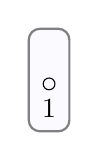
\begin{tikzpicture}
				% 
				\node at (0,0.53) {}; 
				\node at (0,0) [node, label=below:$1$] (1) {};
				% 
				\pgfBox
			\end{tikzpicture} 
		};
		%     \node [above=of K1] {$\rho_0$};
		\node [above] at (K1.north) {$\rho_0$};
		\node [right=of K1](R1) {
			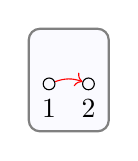
\begin{tikzpicture}
				\node at (0,0.53) {}; 
				\node at (0,0) [node, label=below:$1$] (1) {};
				\node at (.5,0) [node, label=below:$2$] (2) {}; 
				\draw[coloredge] (1) to[out=20, in=160] (2);
				% 
				\pgfBox
			\end{tikzpicture}
		};
		\path (K1) edge[->] node[trans, above] {} (L1);
		\path (K1) edge[->] node[trans, above] {} (R1);
		
		
		\node at (4,2) (L3) {
			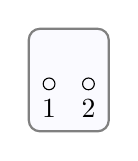
\begin{tikzpicture}
				% 
				\node at (0,0.53) {}; 
				\node at (0,0) [node, label=below:$1$] (1) {} ;
				\node at (0.5,0) [node, label=below:$2$] (2) {} ;
				% 
				\pgfBox
			\end{tikzpicture} 
		};
		\node [right=of L3] (K3) {
			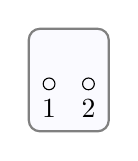
\begin{tikzpicture}
				% 
				\node at (0,0.53) {}; 
				\node at (0,0) [node, label=below:$1$] (1) {} ;
				\node at (0.5,0) [node, label=below:$2$] (2) {} ;
				% 
				\pgfBox
			\end{tikzpicture} 
		};
		%     \node [above=of K3] {$\rho_2$};
		\node [above] at (K3.north) {$\rho_2$};
		\node [right=of K3] (R3) {
			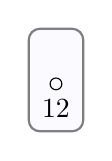
\begin{tikzpicture}
				\node at (0,0.53) {}; 
				\node at (0,0) [node, label=below:$12$] (12) {};
				% 
				\pgfBox
			\end{tikzpicture}
		};
		\path (K3) edge[->] node[trans, above] {} (L3);
		\path (K3) edge[->] node[trans, above] {} (R3);
		
		\node at (8,2) (L2) {
			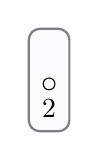
\begin{tikzpicture}
				% 
				\node at (0,0.53) {}; 
				\node at (0,0) [node, label=below:$2$] (1) {} ;
				% 
				\pgfBox
			\end{tikzpicture} 
		};
		\node [right=of L2] (K2) {
			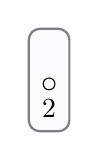
\begin{tikzpicture}
				% 
				\node at (0,0.53) {}; 
				\node at (0,0) [node, label=below:$2$] (1) {};
				% 
				\pgfBox
			\end{tikzpicture} 
		};
		%     \node [above=of K2] {$\rho_1$};
		\node [above] at (K2.north) {$\rho_1$};
		
		\node [right=of K2] (R2) {
			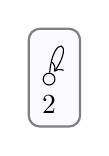
\begin{tikzpicture}
				\node at (0,0) [node, label=below:$2$] (1) {}
				edge [in=55, out=85, loop] ();
				% 
				\pgfBox
			\end{tikzpicture}
		};
		\path (K2) edge[->] node[trans, above] {} (L2);
		\path (K2) edge[->] node[trans, above] {} (R2);
		
		
		%%%%%% second row
		\node at (0,0) (G1) {
			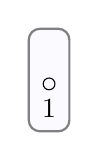
\begin{tikzpicture}
				% 
				\node at (0,0.53) {};
				\node at (0,0) [node, label=below:$1$] (1) {} ;
				% 
				\pgfBox
			\end{tikzpicture} 
		};
		\node [right=of G1] (D1) {
			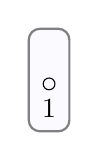
\begin{tikzpicture}
				% 
				\node at (0,0.53) {}; 
				\node at (0,0) [node, label=below:$1$] (1) {};
				% 
				\pgfBox
			\end{tikzpicture} 
		};
		\node at (3,0) (G2) {
			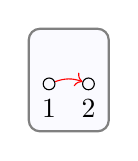
\begin{tikzpicture}
				% 
				\node at (0,0.53) {}; 
				\node at (0,0) [node, label=below:$1$] (1) {} ;
				\node at (0.5,0) [node, label=below:$2$] (2) {} ;
				\draw[coloredge] (1) to[out=20, in=160] (2);
				% 
				\pgfBox
			\end{tikzpicture} 
		};
		\path (D1) edge[->] node[trans, above] {} (G1);
		\path (D1) edge[->] node[trans, above] {} (G2);
		\path (L1) edge[->] node[trans, above] {} (G1);
		\path (K1) edge[->] node[trans, above] {} (D1);
		\path (R1) edge[->] node[trans, above] {} (G2);
		
		\node at (5.5,0) (D2) {
			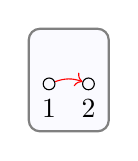
\begin{tikzpicture}
				% 
				\node at (0,0.53) {};
				\node at (0,0) [node, label=below:$1$] (1) {} ;
				\node at (0.5,0) [node, label=below:$2$] (2) {} ;
				\draw[coloredge] (1) to[out=20, in=160] (2);
				% 
				\pgfBox
			\end{tikzpicture} 
		};
		\node at (7.4,0) (G3) {
			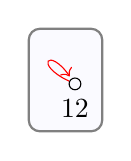
\begin{tikzpicture}
				% 
				\node at (0,0.53) {}; 
				\node at (0,0) [node, label=below:$12$] (12) {}
				edge [in=125, out=155, colorloop] ();
				% 
				\pgfBox
			\end{tikzpicture} 
		};
		
		\path (D2) edge[->] node[trans, above] {} (G2);
		\path (D2) edge[->] node[trans, above] {} (G3);
		\path (L3) edge[->] node[trans, above] {} (G2);
		\path (K3) edge[->] node[trans, above] {} (D2);
		\path (R3) edge[->] node[trans, above] {} (G3);
		
		\node at (9.1,0) (D3) {
			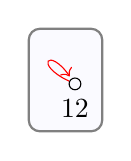
\begin{tikzpicture}
				% 
				\node at (0,0.53) {}; 
				\node at (0,0) [node, label=below:$12$] (12) {}
				edge [in=125, out=155, colorloop] ();
				% 
				\pgfBox
			\end{tikzpicture} 
		};
		\node [right=of D3] (G4) {
			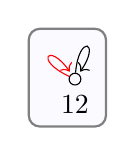
\begin{tikzpicture}
				% 
				\node at (0,0) [node, label=below:$12$] (12) {}
				edge [in=55, out=85, loop] ()
				edge [in=125, out=155, colorloop] ();
				% 
				\pgfBox
			\end{tikzpicture} 
		};
		
		\node[font=\scriptsize, below] at (G1.south) {$G_0$};
		\node[font=\scriptsize, below] at (D1.south) {$D_0$};      
		\node[font=\scriptsize, below] at (G2.south) {$G_1$};
		\node[font=\scriptsize, below] at (D2.south) {$D_1'$};      
		\node[font=\scriptsize, below] at (G3.south) {$G_2'$};
		\node[font=\scriptsize, below] at (D3.south) {$D_2'$};      
		\node[font=\scriptsize, below] at (G4.south) {$G_3$};      
		
		\path (D3) edge[->] node[trans, above] {} (G3);
		\path (D3) edge[->] node[trans, above] {} (G4);
		\path (L2) edge[->] node[trans, above] {} (G3);
		\path (K2) edge[->] node[trans, above] {} (D3);
		\path (R2) edge[->] node[trans, above] {} (G4);
	\end{tikzpicture}
	%
\end{center}
	\end{example}

\begin{remark}\label{rem:switch}

Let $\der{E}=\{\dder{E}_i\}_{i=0}^1$ be a switch for $\dder{D}_0$
and $\dder{D}_1$ along an independence pair $(i_0, i_1)$, then by definition we have an independence pair $(i'_0, i'_1)$ between $\dder{E}_0$ and $\dder{E}_1$ such that
\[
m_0=f_0' \circ i_1'
\quad h_1=g_1' \circ i_0'
\quad m_0'= f_0 \circ i_1
\quad h_1'= g_{1}\circ i_0\]

 The derivation $\der{D}$ uses the same rule of $\der{E}$ in reverse order, thus it is a switch for $\der{E}$ along $(i_0', i_1')$.   Moreover, the same argument shows that if $(\der{E}, \alpha, \omega)$ is a decorated switch for $(\der{D}, \alpha, \omega)$ along $(i_0, i_1)$, then the latter is a decorated switch for the former along $(i'_0, i'_1)$.
\end{remark}

A first property of switches is that they are unique up to abstraction equivalence.

\begin{lemma}[Uniqueness of switches]
	\label{thm:switch_uni}
	Let $\der{D}=\{\dder{D}_{i}\}_{i=0}^1$ be a derivation and suppose
	that both $\der{E}=\{\dder{E}_i\}_{i=0}^1$ and
	$\der{F}=\{\dder{F}_i\}_{i=0}^1$ are switches of $\dder{D}_0$ and
	$\dder{D}_1$. Then there is an abstraction equivalence $\{\phi_X\}_{X\in \Deltamin(\der{E})}$ between $\der{E}$ and $\der{F}$, whose first component is $\id{G_0}$. Moreover, 
	\[\phi_{D_{\der{E}, 0}}\circ j_1=a_1 \qquad \phi_{\der{E}, 1}\circ j_0=a_0\]
\end{lemma}

\begin{proof}
	By definition of switch $\der{E}_0$ and $\der{F}_0$ have the same match $f_0\circ i_1$ and that $\der{E}_1$ and $\der{F}_1$ have the same comatch $g_1\circ i_0$. Thus we get the solid part of the diagram below. If we are able to construct the dotted arrow and prove that they are isomorphism we are done.
	\[\xymatrix@C=22pt{G_{0} && \ar@{>->}[ll]_{f_{\der{F},0}} D_{\der{F},0} \ar[rr]^{g_{\der{F},0}}&& G_{\der{F},1} && \ar@{>->}[ll]_{f_{\der{F},1}} D_{\der{F},1} \ar[rr]^{g_{\der{F},1}}&& G_{2}\\L_1 \ar[d]^{f_0\circ i_1} \ar[u]_{f_0\circ i_1}&& K_{1} \ar[d]^{k_{\der{E},0}} \ar[u]_{k_{\der{F},0}}\ar@{>->}[ll]_{l_1} \ar[r]^{r_1} & R_{1} \ar@/^.35cm/[drrr]|(.315)\hole_(.4){j_0} \ar[dr]|(.3)\hole_{h_{\der{E},0}} \ar@/_.35cm/[urrr]|(.315)\hole^(.4){a_0} \ar[ur]|(.3)\hole^{h_{\der{F},0}}& &L_{0} \ar@/_.35cm/[dlll]^(.4){j_1} \ar[dl]|(.3)\hole^{m_{\der{E},1}} \ar@/^.35cm/[ulll]_(.4){a_1} \ar[ul]|(.3)\hole_{m_{\der{F},1}}& K_{0} \ar[d]_{k_{\der{E},1}} \ar[u]^{k_{\der{F},1}}\ar@{>->}[l]_{l_{0}} \ar[rr]^{r_0} && R_{0} \ar[d]_{g_1\circ i_0} \ar[u]^{g_1\circ i_0}\\ \ar@/^.5cm/[uu]^{\id{G_0}} G_{0} && \ar[ll]^{f_{\der{E},0}} D_{\der{E},0} \ar@{.>}@/^.5cm/[uu]^(.33){\phi_{0}}|\hole \ar[rr]_{g_{\der{E},0}}&& G_{\der{E},1} \ar@{.>}[uu]^(.76){\psi_1}|(.45)\hole |(.55)\hole&& \ar@{>->}[ll]^{f_{\der{E},1}} D_{\der{E},1} \ar@{.>}@/_.5cm/[uu]_(.33){\phi_{1}}|\hole\ar[rr]_{g_{\der{E},1}}&& G_{2}\ar@{.>}@/_.5cm/[uu]_{\psi_2}}\]
	
	Now, by \Cref{prop:unique} we get $\phi_0\colon D_{\der{E},0}\to D_{\der{F},0}$ and $\psi_1 \colon G_{\der{E},1}\to G_{\der{F},1}$ such that the diagram below commutes.
	\[\xymatrix{G_{0} & \ar@{>->}[l]_{f_{\der{F},0}} D_{\der{F},0} \ar[r]^{g_{\der{F},0}}& G_{\der{F},1} \\L_1 \ar[d]^{f_0\circ i_1} \ar[u]_{f_0\circ i_1}& K_{1} \ar[d]^{k_{\der{E},0}} \ar[u]_{k_{\der{F},0}}\ar[l]_{l_1} \ar[r]^{r_1} & R_{1}  \ar[d]_{h_{\der{E},0}}  \ar[u]^{h_{\der{F},0}}\\ \ar@/^.5cm/[uu]^{\id{G_0}} G_{0} & \ar@{>->}[l]^{f_{\der{E},0}} D_{\der{E},0} \ar@/^.5cm/[uu]^(.33){\phi_{0}}|\hole \ar[r]_{g_{\der{E},0}}& G_{\der{E},1} \ar@/_.5cm/[uu]_{\psi_1}}\]
	
	But then we have
	\begin{align*}
		f_{\der{F},0}\circ \phi_0\circ j_1&=f_{\der{E},0} \circ j_1\\&=m_0\\&=f_{\der{F},0}\circ a_1 \end{align*}
	which, since $f_{\der{D},0}$ is mono, entails $a_1= \phi_0\circ j_1$.	This equality, in turn, gives us that
	\begin{align*}
		\psi_1\circ m_{\der{E},1}&=\psi_1 \circ g_{\der{E},0}\circ j_1\\&=g_{\der{F},0}\circ \phi_0\circ j_1\\&=g_{\der{F},0}\circ a_1\\&=m_{\der{F},1}
	\end{align*}
	
	Since $\psi_1$ is an isomorphism, the square below is a pushout. 
	\[\xymatrix@C=35pt{K_0 \ar[d]_{k_{\der{E},1}} \ar@{>->}[r]^{l_0}& L_0 \ar[d]^{\psi_1\circ m_{\der{E},1}}\\D_{\der{E},1} \ar@{>->}[r]_{\psi_1\circ f_{\der{E},1}}& G_{\der{F}, 1}}\]
	
	Moreover, we have already shown that $\psi_1\circ m_{\der{E},1}=m_{\der{F},1}$. Thus, by \Cref{prop:unique} there are the dotted $\phi_1\colon D_{\der{E},1}\to D_{\der{F},1}$ and $\psi_2\colon G_2\to G_2$ as below.
	\[\xymatrix{G_{\der{F},1} & \ar@{>->}[l]_{f_{\der{F},1}} D_{\der{F},1} \ar[r]^{g_{\der{F},1}}& G_2 \\L_0 \ar[d]^{m_{\der{E},1}} \ar[u]_{m_{\der{F},1}}& K_{0} \ar[d]^{k_{\der{E},1}} \ar[u]_{k_{\der{F},1}}\ar@{>->}[l]_{l_1} \ar[r]^{r_1} & R_{0}  \ar[d]_{g_1\circ i_0}  \ar[u]^{g_1\circ i_0}\\ \ar@/^.5cm/[uu]^{\psi_1} G_{\der{E},1} & \ar@{>->}[l]^{f_{\der{E},1}} D_{\der{E},1} \ar@{.>}@/^.5cm/[uu]^(.33){\phi_{1}}|\hole \ar[r]_{g_{\der{E},1}}& G_2 \ar@{.>}@/_.5cm/[uu]_{\psi_2}}\]
	
	To conclude, it is now enough to notice that
	\begin{align*}
		f_{\der{F},1} \circ \phi_1\circ j_0&=\psi_1\circ f_{\der{E},1}\circ j_0\\&=\psi_1\circ h_{\der{E,0}}\\&=h_{\der{F},0}\\&=f_{\der{F},1}\circ a_0
	\end{align*}
	allowing us to deduce $ \phi_1\circ j_0=a_0$.
\end{proof}

Given two sequentially independent direct derivations, it is not necessarily true that a switch for them exists, as shown by the following example. 

\begin{example}\label{ex:diff1}
	Consider the poset $(P, \sqsubseteq)$ depicted below, where
	$P = \mathbb{N} \cup \{a,b,c\}$ and $\sqsubseteq$ is defined by
	$m \sqsubseteq n$ if $m \geq n$, $a \sqsubseteq x$ for all $x \in P$
	and $b, c \sqsubseteq n$ for all $n \in \mathbb{N}$.
	\[\xymatrix@C=16pt@R=1pt{
		& 0 \ar@{-}[dd] \ar@{-}[ddddddl] \ar@{-}[ddddddr] &  \\
		&  & \\
		& 1 \ar@{-}[dd] \ar@{-}[ddddl]  \ar@{-}[ddddr]   &  \\
		&  & \\
		& 2 \ar@{.}[d] \ar@{-}[ddl]   \ar@{-}[ddr]     &  \\
		&  \ar@{.}[dl]   \ar@{.}[dr] & \\
		b \ar@{-}[dr] & & c \ar@{-}[dl]\\
		& a} \]
		
	Let $\X$ be the  
	category associated with this order, which by \Cref{rem:iso} is
	$\mathsf{I(\X)}$-adhesive. Consider a rewriting
	system whose set of rules contains the following 
	\[\xymatrix{a & a \ar[r]^{\sqsubseteq} \ar@{>->}[l]_{\id{a}} & 0 & a & a
		\ar[r]^{\sqsubseteq} \ar@{>->}[l]_{\id{a}} & b }\]
	We can then consider the  following derivation
	$\der{D}=\{\dder{D}_i\}_{i=0}^1$.
	 \[
   \xymatrix@C=25pt{a \ar[d]_{(a,c)}&& \ar@{>->}[d]_{k_0}\ar[ll]_{\id{a}}
		    \ar[r]^{(a,0)} & 0 \ar@/^.35cm/[drrr]|(.315)\hole_(.45){\id{0}}
		    \ar[dr]|(.3)\hole_{\id{0}} && a \ar@/_.35cm/[dlll]^(.45){\hspace{5pt}(a,c)}
		     \ar[dl]|(.3)\hole^{(a,0)}& a \ar[d]^{(a,0)}\ar@{>->}[l]_{\id{a}}
		     \ar[rr]^{(a,b)} && b \ar[d]^{(b,0)}\\c &&
		     \ar@{>->}[ll]^{\id{c}} c \ar[rr]_{(c,0)}&& 0 &&
		     \ar@{>->}[ll]^{\id{0}} 0 \ar[rr]_{\id{0}}&& 0}\]

	Note that the two direct derivations are sequential
	independent. However there is no switch since the rule applied by
	$\dder{D}_1$ cannot be applied to $c$. In fact, there is a unique morphism
	$a\to c$, yielding the diagram
	\[	\xymatrix{a \ar[d]_{(a,c)}& a
		\ar[d]^{(a,c)}\ar@{>->}[l]_{\id{a}} \ar[r]^{(a,b)}& b \\c & c
		\ar@{>->}[l]^{\id{c}}
	}\]
	
	Since $b$ and $c$ do not have a supremum in the poset underlying $\X$, the arrows
	$a\to b$ and $a\to c$ do not have a pushout. Hence we do not get a direct derivation from $c$.
\end{example}



\subsection{Strong-enforcing and well-switching rewriting systems}

\Cref{ex:diff1} show that sequential independence it does not suffice, in general, to guarantee the existence of a switch.  Inspired by the notion of of \emph{canonical filler}
\cite{heindel2009category}, we are now going to give some conditions guaranteeing the existence of a switch. We start proving some technical properties of independence pairs.



\begin{proposition}
	\label{prop:tec}
	Let $(\X,\R)$ be a left-linear rewriting system and
	$(i_0, i_1)$ an independence pair between two direct
	derivations $\dder{D}_0$ and $\dder{D}_1$. Consider the pullback of
	$f_1\colon D_1\mto G_1$ along $g_0\colon D_0\to G_1$ (first
	square below), then there exist the arrows
	$u_1\colon K_1\to P$ and $u_0\colon K_0\to P$ fitting in the
	central and right square. Moreover, the right one is always
	a pullback.
	\[\xymatrix{P \ar@{>->}[r]^{p_0} \ar[d]_{p_1} & D_0
		\ar[d]^{g_0}& K_0 \ar[r]^{r_0} \ar@{.>}[d]_{u_0}& R_0
		\ar[d]^{i_0} & K_1 \ar@{>->}[r]^{l_1} \ar@{.>}[d]_{u_1}&
		L_1 \ar[d]^{i_1}\\ D_1 \ar@{>->}[r]_{f_1} &G_1 &P
		\ar[r]_{p_1} & D_1 &P \ar[r]_{p_0} & D_0}
	\]
\end{proposition}

\begin{proof}
	We start noticing that
	\[\begin{split}
	f_1\circ i_0\circ r_0&=h_0\circ r_0\\&=g_0\circ k_0	\end{split}
	 \qquad\begin{split}
	 	g_0\circ i_1\circ l_1&=m_1\circ l_1\\&= f_1 \circ k_1
	 \end{split}
	\]
	Thus there exists the dotted $u_0\colon K_0\to P$,
	$u_1\colon K_1\to P$ in the diagram
	\[\xymatrix{K_0 \ar[d]_{r_0}
		\ar@{.>}[r]_{u_0}\ar@/^.4cm/[rr]^{k_0} &P
		\ar@{>->}[r]_{p_0} \ar[d]_{p_1}& D_0 \ar[d]^{g_0}&K_1
		\ar@{>->}[d]_{l_1}
		\ar@{.>}[r]_{u_1}\ar@/^.4cm/[rr]^{k_1} &P \ar[r]_{p_1}
		\ar@{>->}[d]_{p_0}& D_1 \ar@{>->}[d]^{f_1}\\R_0
		\ar@/_.4cm/[rr]_{h_0}\ar[r]^{i_0}& D_1
		\ar@{>->}[r]^{f_1}& G_1&L_1
		\ar@/_.4cm/[rr]_{m_1}\ar[r]^{i_1}& D_0 \ar[r]^{g_0}&
		G_1}\]
	By \Cref{prop:pbpoad,lem:pb1} we get that the left half of
	the second rectangle is a pullback.
	\qedhere
\end{proof}

\begin{corollary}\label{lem:cose}Let
		$\der{D}=\{\dder{D}_i\}_{i=0}^1$ be a derivation and suppose
		that $(i_0, i_1)$ is an independence pair between $\dder{D}_0$
		and $\der{D}_1$.  If $\der{E}=\{\dder{E}_i\}_{i=0}^1$ is a
		switch of $\der{D}$ along $(i_0, i_1)$, then there exists
		$q_0\colon P\to D_{\der{E},0}$ in the diagram below. 
		\[\xymatrix{D_{\der{E},0} \ar@{>->}[d]_{f_{\der{E},0}}&P
			\ar@{.>}[l]_{q_0} \ar[r]^{p_1} \ar@{>->}[d]_{p_0}& D_1
			\ar@{>->}[d]^{f_1}\\ G_{0}&D_0 \ar@{>->}[l]^{f_0}\ar[r]_{g_0}&
			G_1}\]
		\end{corollary}
\begin{proof}
	Consider the arrow $u_1\colon K_1\to P$ obtained using
	\Cref{prop:tec}. It fits in the big square on the left
	\[		\xymatrix{K_1 \ar[r]^{u_1} \ar@{>->}[d]_{l_1}&P
		\ar[r]^{\id{P}}\ar@{>->}[d]_{p_0}& P\ar@{>->}[d]^{p_0}\\L_1
		\ar[d]_{\id{L_1}}\ar[r]^{i_1}&D_0 \ar[r]^{\id{D_0}}
		\ar[d]_{\id{D_0}}& D_{0} \ar@{>->}[d]^{f_0}&K_1 \ar@{>->}[d]_{l_1}\ar[r]^{k_{\der{E},0}}&
		D_{\der{E},0} \ar@{>->}[d]^{f_{\der{E},0}} & K_1 \ar[r]^{u_1}
		\ar@{>->}[d]_{l_1}& P \ar@{>->}[d]^{f_0\circ
			p_0}\\
		L_1\ar[r]^{i_1} \ar@/_.4cm/[rr]_{m_{\der{E},0}}&D_0
		\ar@{>->}[r]^{f_0}&G_0 & L_1\ar[r]_{m_{\der{E},0}}&G_0 &L_1
		\ar[r]_{m_{\der{E},0}}&G_0}\]
	
	Since $f_0$ is a monomorphism, every square in the diagram on the left above
	is a pullback. Thus the whole big square is a pullback too.
	Applying \Cref{lem:radj} to the pair of squares on the right now gives
	us the wanted $q_0\colon P\to D_{\der{E},0}$.
\end{proof}


We are now ready to introduce the fundamental concept of this section.

\begin{definition}[Strong independence pair]
	\label{def:strong}
	Let $\X$ be an $\mathcal{M}$-adhesive category 
	and $(\X, \R)$ a left-linear rewriting system. 
	Let also $(i_0, i_1)$ be an independence pair between two direct
	derivations $\dder{D}_0$, $\dder{D}_1$
	as in the solid part of the diagram below
	\[\xymatrix@R=20pt@C=20pt{L_0 \ar[d]_{m_0}&& K_0
	\ar[d]_{k_0}\ar@{>->}[ll]_{l_0} \ar[r]^{r_0} & R_0
	\ar@/^.25cm/[drrr]|(.32)\hole_(.4){i_0}
	\ar[dr]|(.33)\hole_{h_0} && L_1 \ar@/_.25cm/[dlll]^(.4){i_1}
	\ar[dl]|(.33)\hole^{m_1}& K_1 \ar[d]^{k_1}\ar@{>->}[l]_{l_1}
	\ar[rr]^{r_1} && R_1 \ar[d]^{h_1}\\G_0 && \ar@{>->}[ll]^{f_0}
	D_0 \ar[rr]_{g_0}&& G_1 && \ar@{>->}[ll]^{f_1} D_1
	\ar[rr]_{g_1}&& G_2}
\]
	
	We say that $(i_0, i_1)$ is a \emph{strong independence pair} if
	the first two squares depicted  
	below are pushouts and if the pushout of $r_1 : K_1 \to R_1$ along $u_1 : K_1 \to P$ exists.
	\[
	\xymatrix{
		K_0 \ar[r]^{r_0} \ar[d]_{u_0}& R_0 \ar[d]^{i_0} & K_1
		\ar@{>->}[r]^{l_1} \ar[d]_{u_1}& L_1 \ar[d]^{i_1}
		&K_1 \ar[r]^{r_1} \ar[d]_{u_1}& R_1\ar@{.>}[d]^{j_0}
		\\
		%
		P \ar[r]_{p_1} & D_1 &P \ar[r]_{p_0} & D_0
		& P \ar@{.>}[r]_{q_1} & Q_1
	}
	\]
\end{definition}

\begin{remark}\label{rem:deco} 
	Let $(i_0, i_1)$ be a strong
	independence pair between the direct derivations $\dder{D}_0$ and
	$\dder{D}_1$. We can then build the solid part of the diagram
	below
	\[\xymatrix@C=15pt@R=15pt{&&R_0 \ar@/_.8cm/[ddrr]_(.2){i_0}|(.7)\hole
		\ar[dr]^{h_0}&& L_1\ar@/^.8cm/[ddll]^(.2){i_1}
		\ar[dl]_{m_1}\\&K_0\ar[dr]^{k_0}\ar@{>->}[dl]_{l_0}
		\ar@/_.6cm/[ddrr]_(.65){u_0}\ar[ur]^{r_0}&& G_1 && K_1
		\ar@/^.6cm/[ddll]^(.65){u_1}\ar[dl]_{k_1}\ar@{>->}[lu]_{l_1}
		\ar[dr]^{r_1}\\L_0 \ar[dr]^{m_0}
		\ar@{.>}@/_.6cm/[ddrr]_{j_1}&& D_0
		\ar@{>->}[dl]|(.42)\hole_(.64){f_0}\ar[ur]|(.48)\hole^(.7){g_1}&&D_1
		\ar[dr]|(.42)\hole^(.65){g_1}
		\ar@{>->}[ul]|(.48)\hole_(.7){f_1}&&R_1\ar@/^.6cm/[ddll]^{j_0}\ar[dl]^{h_1}\\&G_0
		&&P\ar[dr]^{q_1}
		\ar@{>.>}[dl]_{q_0}\ar[ur]^(.4){p_1}\ar@{>->}[ul]_(.4){p_0}&&G_2\\&&Q_0
		\ar@{>->}@{>.>}[ul]_{a_0} &&Q_1\ar@{.>}[ur]^{b_1}}
	\]
	
	Let us complete this diagram defining the dotted arrows. To get
	$j_1\colon L_0\to Q_0$ and $q_0\colon P\to Q_0$ it is enough to
	take a pushout of $l_0$ along $u_0$, which exists since
	$l_0\in \mathcal{M}$. Moreover, the existence of the wanted
	$a_0\colon Q_0\to G_0$ and $b_1\colon Q_1\to G_2$ follows from
	\[\begin{split}
	f_0\circ p_0 \circ u_0 &= f_0\circ k_0 \\&= m_0\circ l_0
	\end{split}
	 \qquad\begin{split}
	 	g_1\circ p_1\circ u_1 &= g_1\circ k_1\\&=h_1\circ r_1
	 \end{split}
	\]
	We can prove some other properties of
		the arrows appearing in the diagram above. The four rectangles
		below are pushouts and their left halves are pushouts
		too. Therefore, by \Cref{lem:po1} also their right halves are
		pushouts.  Moreover, $q_0$ and $a_0$ are pushouts of
		respectively $l_0$ and $p_0$, thus they are elements of
		$\mathcal{M}$. By \Cref{prop:pbpoad} the left halves of the
		second and third rectangles are pullbacks too.
		
		\[\xymatrix{K_0 \ar@/^.4cm/[rr]^{k_0}\ar[d]_{r_0}\ar[r]_{u_0}
			&P\ar[d]^{p_1} \ar@{>->}[r]_{p_0} & D_0 \ar[d]^{g_0}&K_1
			\ar@/^.4cm/[rr]^{k_1}\ar@{>->}[d]_{l_1}\ar[r]_{u_1}
			&P\ar@{>->}[d]^{p_0} \ar[r]_{p_1} & D_1 \ar@{>->}[d]^{f_1}\\
			R_0 \ar@/_.4cm/[rr]_{h_0} \ar[r]^{i_0}&D_1 \ar@{>->}[r]^{f_1}
			& G_1&L_1 \ar@/_.4cm/[rr]_{m_1} \ar[r]^{i_1}&D_0\ar[r]^{g_0} &
			G_1}\]
			\[\xymatrix{K_0
			\ar@/^.4cm/[rr]^{k_0}\ar@{>->}[d]_{l_0}\ar[r]_{u_0}
			&P\ar@{>->}[d]^{q_0} \ar@{>->}[r]_{p_0} & D_0
			\ar@{>->}[d]^{f_0}&K_1
			\ar@/^.4cm/[rr]^{k_1}\ar[d]_{r_1}\ar[r]_{u_1}
			&P\ar[d]^{q_1} \ar[r]_{p_1} & D_1 \ar[d]^{g_1}\\
			L_0 \ar@/_.4cm/[rr]_{m_0} \ar[r]^{j_1}&Q_0 \ar@{>->}[r]^{a_0}
			& G_0&R_1 \ar@/_.4cm/[rr]_{h_1} \ar[r]^{j_0}&Q_1 \ar[r]^{b_1}
			& G_2}\]
\end{remark}

So equipped we can now prove a version of the Local Church-Rosser Theorem for strong independence pairs in ledt-linear DPO rewriting systems.

\begin{theorem}[Local Church-Rosser Theorem]\label{prChurch} Let $\X$ be an $\mathcal{M}$-adhesive category and $(\X, \R)$ a left-linear DPO rewriting system on it. If $(i_0, i_1)$ is a strong independence pair
	between $\dder{D}_0$ and $\dder{D}_1$, then there exists a switch of $\dder{D}_0$ and $\dder{D}_1$ along it.
\end{theorem}
\begin{proof}
	Let us begin considering the diagram
	built in \Cref{rem:deco}
	\[\xymatrix@C=15pt@R=15pt{&&R_0
		\ar@/_.8cm/[ddrr]_(.2){i_0}|(.7)\hole \ar[dr]^{h_0}&&
		L_1\ar@/^.8cm/[ddll]^(.2){i_1}
		\ar[dl]_{m_1}\\&K_0\ar[dr]^{k_0}\ar@{>->}[dl]_{l_0}
		\ar@/_.6cm/[ddrr]_(.65){u_0}\ar[ur]^{r_0}&& G_1 && K_1
		\ar@/^.6cm/[ddll]^(.65){u_1}\ar[dl]_{k_1}\ar@{>->}[lu]_{l_1}
		\ar[dr]^{r_1}\\L_0 \ar[dr]^{m_0} \ar@{>}@/_.6cm/[ddrr]_{j_1}&& D_0
		\ar@{>->}[dl]|(.42)\hole_(.64){f_0}\ar[ur]|(.48)\hole^(.7){g_1}&&D_1
		\ar[dr]|(.42)\hole^(.65){g_1}
		\ar@{>->}[ul]|(.48)\hole_(.7){f_1}&&R_1\ar@/^.6cm/[ddll]^{j_0}\ar[dl]_{h_1}\\&G_0
		&&P\ar[dr]^{q_1}
		\ar@{>->}[dl]_{q_0}\ar[ur]^(.4){p_1}\ar@{>->}[ul]_(.4){p_0}&&G_2\\&&Q_0
		\ar@{>->}@{>->}[ul]_{a_0} \ar@{.>}[dr]_{b_0} &&Q_1\ar[ur]^{b_1}
		\ar@{>.>}[dl]^{a_1} \\ &&&H_1 }\] 
		
		Since $q_0\colon P\to Q_0$ is in
	$\mathcal{M}$, we can take its pushout along $q_1$ to get the dotted
	arrows $a_1\colon Q_1\mto H_1$ and $q_0\colon Q_0\to H_1$. But then,
	since the composite of two pushout squares is a pushout, the diagram
	below is a derivation
	\[\xymatrix{L_1 \ar[d]_{f_0 \circ i_1}&& K_1
		\ar[d]_{q_0\circ u_1}\ar@{>->}[ll]_{l_1} \ar[r]^{r_1} & R_1
		\ar@/^.35cm/[drrr]|(.31)\hole_(.4){j_0} \ar[dr]|(.3)\hole_{a_1\circ
			j_0} && L_0 \ar@/_.35cm/[dlll]^(.4){j_1} \ar[dl]|(.3)\hole^{b_0\circ
			j_1}& K_0 \ar[d]^{q_1\circ u_0}\ar@{>->}[l]_{l_0} \ar[rr]^{r_0} && R_0
		\ar[d]^{g_1\circ i_0} \\G_0 && \ar@{>->}[ll]^{a_0} Q_0 \ar[rr]_{b_0}&&
		H_1 && \ar@{>->}[ll]^{a_1} Q_1 \ar[rr]_{b_1}&& G_2}\] 
		
		The thesis now follows at once since, by construction, the derivation above is a switch of $\dder{D}_0$ and $\dder{D}_1$ along	$(i_0, i_1)$.
\end{proof}

The previous theorem not only assures about the existence of a switch along a strong independence pair, but it provides us with an explicit description of it. In turn this, using \Cref{thm:switch_uni}, allows us to deduce some property common to all switches along strong independence pairs.  

\begin{lemma}\label{cor:strongip}
	Let $(\X, \R)$ be a left-linear DPO rewriting system and consider the following derivation $\der{D}={\dder{D}_{i}}_{i=0}^i$ and suppose that $(i_0, i_1)$ is a strong independence pair.
	\[\xymatrix@R=20pt@C=20pt{L_0 \ar[d]_{m_0}&& K_0
		\ar[d]_{k_0}\ar@{>->}[ll]_{l_0} \ar[r]^{r_0} & R_0
		\ar@{.>}@/^.25cm/[drrr]|(.32)\hole_(.4){i_0}
		\ar[dr]|(.33)\hole_{h_0} && L_1 \ar@{.>}@/_.25cm/[dlll]^(.4){i_1}
		\ar[dl]|(.33)\hole^{m_1}& K_1 \ar[d]^{k_1}\ar@{>->}[l]_{l_1}
		\ar[rr]^{r_1} && R_1 \ar[d]^{h_1}\\G_0 && \ar@{>->}[ll]^{f_0}
		D_0 \ar[rr]_{g_0}&& G_1 && \ar@{>->}[ll]^{f_1} D_1
		\ar[rr]_{g_1}&& G_2}
	\]
	
	Suppose, moreover, that the following diagram defines a switch for $\dder{D}_0$ and $\dder{D}_1$ along $(i_0, i_1)$. 	
	\[
	\xymatrix@R=20pt@C=20pt{
		{L_1} \ar[d]_{m_0'}
		&&  {K_1} \ar@{>->}[ll]_{l_1} \ar[r]^{r_1} \ar[d]_{k_0'}
		&  {R_1} \ar[dr]|(.33)\hole_{h_0'}  \ar@/^.25cm/@{.>}_(.4){i_0'}|(.32)\hole[drrr]
		& & 
		{L_0}\ar[dl]|(.33)\hole^{m_1'} \ar@/_.25cm/@{.>}^(.4){i_1'}[dlll] 
		&  {K_0} \ar@{>->}[l]_{l_0} \ar[rr]^{r_0} \ar[d]^{k_1'}
		& & {R_0} \ar[d]^{h_1'} \\		
		{G_0}
		& & {D_0'} \ar@{>->}[ll]^{f_0'} \ar[rr]_{g_0'}
		& &  {G'_1} 
		& &  {D_1'} \ar@{>->}[ll]^{f_1'} \ar[rr]_{g_1'}
		& & {G_2}  }
	\]
and define $T$, with the arrows $t_0\colon T\mto D'_0$ and $t_1\colon T\to D'_1$ as the pullback of $f'_1$ along $g'_0$.


Finally, consider the derivation $\der{F}$ below, constructed in the proof of \Cref{prChurch}. 
\[\xymatrix{L_1 \ar[d]_{f_0 \circ i_1}&& K_1
	\ar[d]_{q_0\circ u_1}\ar@{>->}[ll]_{l_1} \ar[r]^{r_1} & R_1
	\ar@/^.35cm/[drrr]|(.31)\hole_(.4){j_0} \ar[dr]|(.3)\hole_{a_1\circ
		j_0} && L_0 \ar@/_.35cm/[dlll]^(.4){j_1} \ar[dl]|(.3)\hole^{b_0\circ
		j_1}& K_0\ar[d]^{q_1\circ u_0}\ar@{>->}[l]_{l_0} \ar[rr]^{r_0} && R_0
	\ar[d]^{g_1\circ i_0} \\G_0 && \ar@{>->}[ll]^{a_0} Q_0 \ar[rr]_{b_0}&&
	H_1 && \ar@{>->}[ll]^{a_1} Q_1 \ar[rr]_{b_1}&& G_2}\]
and let $\{\phi_{X}\}_{X\in \Deltamin(\der{F})}$ be the abstraction equivalence built in \Cref{thm:switch_uni}.

	Then the following hold true:
	\begin{enumerate}
		\item consider the following two squares, the first of which is a pullback and the second an $\mathcal{M}$-pushout,
		\[\xymatrix{P \ar[r]^{p_1} \ar@{>->}[d]_{p_0} & D_1 \ar@{>->}[d]^{f_1}& P \ar[r]^{q_1} \ar@{>->}[d]_{q_0} & Q_1 \ar@{>->}[d]^{a_1}\\ D_0 \ar[r]_{g_0} & G_1&Q_0 \ar[r]_{b_0} & H_1}\]
		then there exists an isomorphism $v\colon P\to T$ fitting in the diagram below:
		\[\xymatrix{ P \ar@{.>}[dr]^{v} \ar[rrr]^{q_1} \ar@{>->}[ddd]_{q_0}&&& Q_1 \ar@{>->}[ddd]^{a_1} \ar[dl]_{\phi_{Q_1}}\\&T \ar@{>->}[d]_{t_0}\ar[r]^{t_1}& D'_1 \ar@{>->}[d]^{f'_1} \\ & D'_0\ar[r]_{g'_0} & G'_1\\Q_0 \ar[rrr]_{b_0} \ar[ur]_{\phi_{Q_0}}&&& H_1 \ar[ul]^{\phi_{H_1}}}\]
		
		\item consider the diagram below, in which the inner square is a pullback and the dotted arrows are constructed as in \Cref{rem:deco}:
		\[\xymatrix{K_1 \ar[r]^{r_1} \ar@/_.3cm/[ddr]_{k'_0} \ar@{.>}[dr]^{e_0}& R_1  \ar[dr]^{i'_0}  && K_0 \ar@{>->}[r]^{l_0} \ar@/_.3cm/[ddr]_{k'_1} \ar@{.>}[dr]^{e_1}& L_1  \ar[dr]^{i'_1} \\& T\ar@{>->}[d]_{t_0} \ar[r]^{t_1}& D'_1  \ar@{>->}[d]^{f'_1} && T \ar@{>->}[r]^{t_0} \ar[d]_{t_1}& D'_0 \ar[d]^{g'_0}\\&D'_0 \ar[r]_{g'_0} & G'_1 && D'_1\ar@{>->}[r]_{f'_1} & G'_1}\]
		then $v\circ u_1=e_0$, $v\circ u_0=e_1$ and the two squares below are pushouts;
		\[\xymatrix{K_1  \ar[d]_{e_0} \ar[r]^{r_1} & R_1 \ar[d]^{i'_0} & K_0 \ar@{>->}[r]^{l_0} \ar[d]_{e_1}& L_0 \ar[d]^{i'_1}\\ T \ar[r]_{t_1}  & D'_1 & T \ar@{>->}[r]_{t_0} & D'_0 }\]
				
	\item $(i'_0, i'_1)$ is a strong independence pair;
	
	\item there exists a commutative diagram the one below.
	
	\[\xymatrix@C=15pt@R=15pt{&&R_0 \ar@/_.8cm/[ddrr]_(.2){i_0}|(.7)\hole
		\ar[dr]^{h_0}&& L_1\ar@/^.8cm/[ddll]^(.2){i_1}
		\ar[dl]_{m_1}\\&K_0\ar[dr]^{k_0}\ar@{>->}[dl]_{l_0}
		\ar@/_.6cm/[ddrr]|(.36)\hole^(.65){u_0}\ar[ur]^{r_0}&& G_1 &&
		K_1
		\ar@/^.6cm/[ddll]|(.36)\hole_(.65){u_1}\ar[dl]_{k_1}\ar@{>->}[lu]_{l_1}
		\ar[dr]^{r_1}\\L_0
		\ar@/_.6cm/[ddrr]_(.2){i'_1}|(.31)\hole|(.81)\hole
		\ar[dr]^(.4){m_0}|(.61)\hole && D_0
		\ar@{>->}[dl]|(.4)\hole_(.65){f_0}\ar[ur]|(.5)\hole^(.7){g_0}&&D_1
		\ar[dr]|(.4)\hole^(.65){g_1}
		\ar@{>->}[ul]|(.5)\hole_(.65){f_1}&&R_1\ar@/^.6cm/[ddll]^(.2){i'_0}|(.31)\hole|(.81)\hole\ar[dl]_{h_1}|(.6)\hole\\&G_0
		&&P\ar@{.>}[dr]_{z_1}	\ar@{>.>}[dl]^{z_0}\ar[ur]^(.4){p_1}\ar@{>->}[ul]_(.4){p_0}&&G_2\\L_1	\ar@/^.6cm/[uurr]^(.2){i_1} \ar[ur]_(.35){m'_0}|(.61)\hole && D'_0	\ar@{>->}[ul]|(.4)\hole_(.65){f'_0}\ar[dr]|(.5)\hole_(.65){g'_0}	&&D'_1\ar[ur]|(.4)\hole^(.65){g'_1} \ar@{>->}[dl]|(.5)\hole^(.65){f'_1}	&& R_0 \ar[ul]^(.35){h'_1}|(.61)\hole\ar@/_.6cm/[uull]_(.2){i_0}\\ &K_1	\ar[ur]_{k'_0} \ar[dr]_{r_1}	\ar@{>->}[ul]^{l_1}\ar@/^.6cm/[uurr]_(.65){u_1}&&G'_1&& K_0\ar[ur]_{r_0} \ar[ul]^{k'_1} \ar@{>->}[dl]^{l_0} \ar@/_.6cm/[uull]^(.65){u_0}\\&& R_1	\ar[ur]_{h'_0}\ar@/^.8cm/[uurr]^(.2){i'_0}&& L_0 \ar[ul]^{m'_1} \ar@/_.8cm/[uull]_(.2){i'_1} |(.69)\hole }\] 
	in which the following four squares are all pushouts, while the first three are also pullbacks.
	\[\xymatrix{P \ar@{>->}[r]^{p_0} \ar@{>->}[d]_{p_1}& D_0 \ar@{>->}[d]^{g_0}  & P \ar@{>->}[r]^{z_0} \ar@{>->}[d]_{p_0}& D'_0 \ar@{>->}[d]^{f'_0} &  P \ar@{>->}[d]_{z_0} \ar[r]^{z_1} & D'_1 \ar@{>->}[d]^{f'_1} & P\ar[r]^{z_1} \ar[d]_{p_1}&D'_1 \ar[d]^{g'_1}\\ D_1 \ar@{>->}[r]_{f_1} & G_1  & D_0 \ar@{>->}[r]_{f_0} & G_0 & D'_0 \ar[r]_{g'_0}& G'_1 & D_1 \ar[r]_{g_1}& G_2}\]	
	\end{enumerate}
\end{lemma}
\begin{proof}
	\begin{enumerate}
		\item  By \Cref{prop:pbpoad}, the square below is also a pullback.
			\[\xymatrix{P \ar[r]^{q_1} \ar@{>->}[d]_{q_0} & Q_1 \ar@{>->}[d]^{a_1}\\ Q_0 \ar[r]_{b_0} & H_1}\]
			Thus by the universal property of pullbacks  we get the dotted arrows $v\colon P\to T$ and $w\colon T\to P$ in the following diagrams.
		\[\xymatrix{ P \ar@{.>}[dr]^{v} \ar[rrr]^{q_1} \ar@{>->}[ddd]_{q_0}&&& Q_1 \ar@{>->}[ddd]^{a_1} \ar[dl]_{\phi_{Q_1}}& T\ar@{.>}[dr]^{w}  \ar[rrr]^{t_1} \ar@{>->}[ddd]_{t_0}&&& D'_1 \ar[dl]_{\phi^{-1}_{Q_1}} \ar@{>->}[ddd]^{f'_1}\\&T \ar@{>->}[d]_{t_0}\ar[r]^{t_1}& D'_1 \ar@{>->}[d]^{f'_1} &&& P \ar@{>->}[d]_{q_0}\ar[r]^{q_1}& Q_1\ar@{>->}[d]^{a_1}\\ & D'_0\ar[r]_{g'_0} & G'_1 &&& Q_0 \ar[r]_{b_0}& H_1 \\Q_0 \ar[rrr]_{b_0} \ar[ur]_{\phi_{Q_0}}&&& H_1 \ar[ul]^{\phi_{H_1}} & D'_0 \ar[rrr]_{g'_0} \ar[ur]_{\phi^{-1}_{Q_0}}&&&G'_1 \ar[ul]^{\phi^{-1}_{H_1}}}\]

To see that they are one the inverse of the other it is then enough to compute.
		\[\begin{split}
		t_0\circ v\circ w &=\phi_{Q_0}\circ q_0\circ w\\&=\phi_{Q_0}\circ \phi^{-1}_{Q_0} \circ t_0\\&=t_0\\q_0\circ w\circ v&=\phi^{-1}_{Q_0}	\circ t_0\circ v\\&=\phi^{-1}_{Q_0} \circ \phi_{Q_0}\circ q_0\\&=q_0 	\end{split}\qquad \begin{split}
		t_1\circ v\circ w &=\phi_{Q_1}\circ q_1\circ w\\&=\phi_{Q_1}\circ \phi^{-1}_{Q_1} \circ t_1\\&=t_1\\q_1\circ w\circ v&=\phi^{-1}_{Q_1}	\circ t_1\circ v\\&=\phi^{-1}_{Q_1} \circ \phi_{Q_1}\circ q_1\\&=q_1
		\end{split}\]
		
	\item By \Cref{thm:switch_uni}, we know that $\phi_{G_0}=\id{G_0}$, so that $a_0=f'_0\circ \phi_{Q_0}$, moreover, by the same theorem we have 
	\[\phi_{Q_1}\circ j_0=i'_0 \qquad  \phi_{Q_0}\circ j_1=i'_1\] 
		
		We can now use the previous equalities to get
		\[\begin{split}
			t_0\circ v\circ u_0&=\phi_{Q_0} \circ q_0\circ u_0\\&=\phi_{Q_0}\circ j_1\circ l_0\\&=i'_1\circ l_0\\&=t_0\circ e_1\\	t_0\circ v\circ u_1&=\phi_{Q_0} \circ q_0\circ u_1\\&=k'_0\\&= t_0\circ e_0
		\end{split} \qquad \begin{split}
			t_1\circ v\circ u_1&=\phi_{Q_1} \circ q_1\circ u_1\\&=\phi_{Q_1}\circ j_0\circ r_1\\&=i'_0\circ r_1\\&= t_1\circ e_0 \\ t_1\circ v\circ u_0&=\phi_{Q_1} \circ q_1\circ u_0\\&=k'_1\\&=t_1\circ e_1
		\end{split}\]
		
	So that $v\circ u_1=e_0$ and $v\circ u_0=e_1$. The thesis now follows from the two diagrams below, since their left halves are pushouts by construction.		
		\[\xymatrix{K_1  \ar@/^.4cm/[rr]^{e_0}\ar[r]_{u_1} \ar[d]_{r_1}& P \ar[r]_{v} \ar[d]_{q_1} & T \ar[d]^{t_1} & K_0 \ar@/^.4cm/[rr]^{e_1} \ar@{>->}[d]_{l_0}\ar[r]_{u_0} & P \ar[r]_{v}  \ar@{>->}[d]_{q_0}& T \ar@{>->}[d]^{t_0}\\ R_1 \ar@/_.4cm/[rr]_{i'_0} \ar[r]^{j_0}& Q_1 \ar[r]^{\phi_{Q_1}} & D'_1 & L_0 \ar@/_.4cm/[rr]_{i'_1} \ar[r]^{j_0} & Q_0 \ar[r]^{\phi_{Q_0}} & D'_0 }\]
		
	
		\item Given the results of the previous point, it is now enough to show that the pushout of $r_0\colon K_0\to R_0$ along $e_1\colon K_0\to T$ exists. We can consider the diagram below
		\[\xymatrix{K_0 \ar@/^.4cm/[rr]^{u_0} \ar[d]_{r_0} \ar[r]_{e_1}& T  \ar[d]_{p_1\circ w}\ar[r]_{w} & P \ar[d]^{p_1}\\ R_0 \ar[r]_{i_0}& D_1 \ar[r]_{\id{D_1}}& D_1}\]
		But the outer diagram is a pushout since $(i_0, i_1)$ is strong and we can conclude. 
		
		
		
		\item Let $z_0\colon P\mto D'_0$ and $z_1\colon P\to D_1$ be, respectively, $t_0\circ v$ and $t_1\circ v$. Then we have
		
		\[\begin{split}
		g'_0\circ z_0&=g'_0\circ t_0\circ v\\&=f'_1\circ t_1\circ v\\&=f'_1\circ z_1
		\end{split}\quad \begin{split}
		z_0\circ u_1&=t_0\circ v\circ u_1\\&=\phi_{Q_0}\circ q_0\circ u_1\\&=k'_0
		\end{split} \quad \begin{split}
		z_1\circ u_0&=t_1\circ v\circ u_0\\&=\phi_{Q_1}\circ q_1\circ u_0\\&=k'_1
		\end{split}\]
		
		Moreover
		\[\begin{split}
			f'_0\circ z_0&=f'_0\circ t_0\circ v\\&=f'_0\circ \phi_{Q_0}\circ q_0\\&=a_0\circ q_0\\&=f_0\circ p_0
		\end{split} \qquad \begin{split}
		g'_1\circ z_1=g'_1\circ t_1\circ v\\&=g'_1\circ \phi_{Q_1}\circ q_1\\&=\phi_{G_2}\circ b_1 \circ q_1\\&=\phi_{G_2}\circ g_1\circ p_1\\&=f_0\circ p_0
		\end{split} \]
		
		
		Therefore the $z_0$ and $z_1$ fit in the diagram above.
		
		To conclude, notice that the the four rectangles below and their halves, by construction and by point $3$, are pushouts, thus by \Cref{lem:po1} also their right halves are
		pushouts. 
		
		\[\xymatrix{K_0 \ar@/^.4cm/[rr]^{k_0}\ar[d]_{r_0}\ar[r]_{u_0}
			&P\ar[d]^{p_1} \ar@{>->}[r]_{p_0} & D_0 \ar[d]^{g_0}&K_0
			\ar@/^.4cm/[rr]^{k'_1}\ar@{>->}[d]_{l_0}\ar[r]_{u_0}
			&P\ar@{>->}[d]^{z_0} \ar[r]_{z_1} & D'_1 \ar@{>->}[d]^{f'_1}\\
			R_0 \ar@/_.4cm/[rr]_{h_0} \ar[r]^{i'_1}&D_1 \ar@{>->}[r]^{f_1}
			& G_1&L_1 \ar@/_.4cm/[rr]_{m'_1} \ar[r]^{i_1}&D'_0\ar[r]^{g'_0} &
			G'_1}\]
		\[\xymatrix{K_0
			\ar@/^.4cm/[rr]^{k_0}\ar@{>->}[d]_{l_0}\ar[r]_{u_0}
			&P\ar@{>->}[d]^{z_0} \ar@{>->}[r]_{p_0} & D_0
			\ar@{>->}[d]^{f_0}&K_1
			\ar@/^.4cm/[rr]^{k_1}\ar[d]_{r_1}\ar[r]_{u_1}
			&P\ar[d]^{z_1} \ar[r]_{p_1} & D_1 \ar[d]^{g_1}\\
			L_0 \ar@/_.4cm/[rr]_{m_0} \ar[r]^{i'_1}&D'_0 \ar@{>->}[r]^{f'_0}
			& G_0&R_1 \ar@/_.4cm/[rr]_{h_1} \ar[r]^{i'_0}&D'_1 \ar[r]^{b_1}
			& G_2}\]
			
			We conclude by \Cref{prop:pbpoad}. \qedhere 
	\end{enumerate}
\end{proof}


We can now turn to prove the fundamental property that we need to rely upon:  any decorated switch along a strong independence pair induces a consistent permutation.

\begin{lemma}\label{lem:switchtoperm}
	Let $(\der{D}, \alpha, \omega)$ be a decorated derivations of length $2$ and suppose that $(\der{E}, \alpha, \omega)$ is a decorated switch for it along the independence pair $(i_0, i_1)$. Then there exists an arrow $\kappa\colon G_1\to \tpro{E}$ such that 
		\[\kappa \circ g_{0} = \iota_{\der{E}, G_0}\circ f_{0} \qquad \kappa\circ h_{0}= \iota_{\der{E}, R_0}\]
		
		Moreover, if $(i_0, i_1)$ is strong, also the following facts are true:
		\begin{enumerate}
		\item there exists an arrow $\phi\colon \tpro{D}\to \tpro{E}$ such that
		\[\phi \circ \iota_{\der{D}, G_0}=\iota_{\der{E}, G_0} \qquad \phi \circ \iota_{\der{D}, G_1}=\kappa \qquad \phi \circ \iota_{\der{D}, G_2}=\iota_{\der{E}, G_2}\]
		\item the $2$-cycle $\tau_{0,1}\colon [0,1]\to [0,1]$ is a consistent permutation between $(\der{D}, \alpha, \omega)$ and $(\der{E}, \alpha, \omega)$.
	\end{enumerate}
\end{lemma}
\begin{proof}
	To fix the notation let $\der{D}$ be given by the first diagram below and $\der{E}$ by the second one.
	\[\xymatrix@R=20pt@C=20pt{L_0 \ar[d]_{m_0}&& K_0
		\ar[d]_{k_0}\ar@{>->}[ll]_{l_0} \ar[r]^{r_0} & R_0
		\ar@{>}@/^.25cm/[drrr]|(.32)\hole_(.4){i_0}
		\ar[dr]|(.33)\hole_{h_0} && L_1 \ar@{>}@/_.25cm/[dlll]^(.4){i_1}
		\ar[dl]|(.33)\hole^{m_1}& K_1 \ar[d]^{k_1}\ar@{>->}[l]_{l_1}
		\ar[rr]^{r_1} && R_1 \ar[d]^{h_1}\\G_0 && \ar@{>->}[ll]^{f_0}
		D_0 \ar[rr]_{g_0}&& G_1 && \ar@{>->}[ll]^{f_1} D_1
		\ar[rr]_{g_1}&& G_2}
	\]
	\[
	\xymatrix@R=20pt@C=20pt{
		{L_1} \ar[d]_{m_0'}
		&&  {K_1} \ar@{>->}[ll]_{l_1} \ar[r]^{r_1} \ar[d]_{k_0'}
		&  {R_1} \ar[dr]|(.33)\hole_{h_0'}  \ar@/^.25cm/@{>}_(.4){i_0'}|(.32)\hole[drrr]
		& & 
		{L_0}\ar[dl]|(.33)\hole^{m_1'} \ar@/_.25cm/@{>}^(.4){i_1'}[dlll] 
		&  {K_0} \ar@{>->}[l]_{l_0} \ar[rr]^{r_0} \ar[d]^{k_1'}
		& & {R_0} \ar[d]^{h_1'} \\		
		{G_0}
		& & {D_0'} \ar@{>->}[ll]^{f_0'} \ar[rr]_{g_0'}
		& &  {G'_1} 
		& &  {D_1'} \ar@{>->}[ll]^{f_1'} \ar[rr]_{g_1'}
		& & {G_2}  }
	\]
	
 $G_1$ is obtained as the pushout of $k_0$ along $r_0$m thus get the wanted arrow $\kappa\colon G_1\to \tpro{E}$ it is now enough to compute:
	\begin{align*}
		\iota_{\der{E}, G_0}\circ f_{0}\circ  k_{0}&= \iota_{\der{E}, G_0}\circ m_{0} \circ l_{ 0}\\&=\iota_{\der{E}, G_0}\circ  f'_{0} \circ i'_1 \circ l_0\\&=\iota_{\der{E}, D'_0}\circ i'_1 \circ l_0\\&=\iota_{\der{E}, G'_1} \circ g'_0\circ m'_1 \circ l_0\\&=\iota_{\der{E}, G'_1}\circ m'_1\circ l_0	\\&=\iota_{\der{E}, G'_1} \circ f'_1\circ k'_1\\&=\iota_{\der{E}, D'_1}\circ k'_1\\&=\iota_{\der{E}, K'_0}\\&= \iota_{\der{E}, R_0} \circ r_0
	\end{align*}
	
	Let us now suppose that $(i_0,i_1)$ is a strong independence pair. We can then consider the following two squares, the first of which is a pullback and the second one, by strongness, a  pushout.
	
			\[\xymatrix{P \ar[r]^{p_1}  \ar@{>->}[d]_{p_0} & D_1 \ar@{>->}[d]^{f_1} & K_0 \ar[r]^{r_0}  \ar[d]_{u_0} & R_0 \ar[d]^{i_0}\\ D_0\ar[r]_{g_0} & G_1 & P\ar[r]_{p_1} & D_1}\]

	\begin{enumerate}
		\item   Consider the arrow $\kappa\colon G_1\to \tpro{E}$ built in the previous point, then we have
		\begin{align*}
			\kappa \circ f_1\circ i_0&=\kappa\circ h_0\\&=\iota_{\der{E},R_0}\\&=\iota_{\der{E}{G_2}}\circ h'_1\\&=\iota_{\der{E}{G_2}}\circ g_1\circ i_0
		\end{align*}
		
		\begin{align*}
			\kappa\circ f_1\circ p_1&=\kappa \circ g_0\circ p_0\\&=\iota_{\der{E},G_0}\circ f_0\circ p_0
		\end{align*}
		\item 
		\qedhere 
	\end{enumerate}
\end{proof}

\Cref{prChurch} and \Cref{lem:switchtoperm} guarantees some basic but fundamental properties of switches whithout which developing a theory of concurrency seems hopeless, we are thus lead to the following definition.

\begin{definition}
A left-linear DPO rewriting system $(\X, \R)$ is \emph{strong enforcing} if every independence pair is strong.
\end{definition}

The notion of strong enforcing DPO rewriting system encompasses that of linear one.


\begin{proposition}\label{prop:linstrong}
	Every linear rewriting system $(\X, \R)$ is strong enforcing.
\end{proposition}
\begin{proof}
	Suppose that $\X$ is $\mathcal{M}$-adhesive and let $(i_0, i_1)$ be
	an independence pair as below
	\[
	\xymatrix@C=15pt{L_0 \ar[d]_{m_0}&& K_0
		\ar[d]_{k_0}\ar@{>->}[ll]_{l_0} \ar@{>->}[r]^{r_0} & R_0
		\ar@/^.35cm/[drrr]|(.3)\hole_(.4){i_0} \ar[dr]|(.3)\hole_{h_0}
		&& L_1 \ar@/_.35cm/[dlll]^(.4){i_1} \ar[dl]|(.3)\hole^{m_1}& K_1
		\ar[d]^{k_1}\ar@{>->}[l]_{l_1} \ar@{>->}[rr]^{r_1} && R_1
		\ar[d]^{h_1} \\G_0 && \ar@{>->}[ll]^{f_0} D_0
		\ar@{>->}[rr]_{g_0}&& G_1 && \ar@{>->}[ll]^{f_1} D_1
		\ar@{>->}[rr]_{g_1}&& G_2}\]
	
	Since $(\X, \R)$ is linear, then $r_1\colon K_1\to R_1$ belongs to
	$\mathcal{M}$, thus it admits a pushout along $u_1\colon K_1\to P$,
	as desired. Moreover, let us consider the two rectangles below
	\[
	\xymatrix{K_0 \ar@/^.4cm/[rr]^{k_0}\ar@{>->}[d]_{r_0}\ar[r]_{u_0}
		&P\ar@{>->}[d]^{p_1} \ar@{>->}[r]_{p_0} & D_0
		\ar@{>->}[d]^{f_0}& K_1
		\ar@/^.4cm/[rr]^{k_1}\ar@{>->}[d]_{l_1}\ar[r]_{u_1}
		&P\ar@{>->}[d]^{p_0} \ar@{>->}[r]_{p_1} & D_1
		\ar@{>->}[d]^{f_1}\\ R_0 \ar@/_.4cm/[rr]_{h_0} \ar[r]^{i_0}&D_1
		\ar@{>->}[r]^{f_1} & G_1& L_1 \ar@/_.4cm/[rr]_{m_1}
		\ar[r]^{i_1}&D_0 \ar@{>->}[r]^{g_0} & G_1} \] By hypothesis
	$r_0$ and $l_1$ are in $\mathcal{M}$, thus $f_1$ and $g_0$ belong to
	it too. The first point of \Cref{lem:popb} yields the thesis.
\end{proof}

We can easily 

\begin{lemma}
Let $(P, \{p_0, p_1\})$ be the pullback of $f_1$ along $g_1$, then there exists $z_0\colon P\mto D'_0$ and $z_1\colon P\to D'_1$ making the following diagram commutative
\[\xymatrix@C=15pt@R=15pt{&&R_0 \ar@/_.8cm/[ddrr]_(.2){i_0}|(.7)\hole
	\ar[dr]^{h_0}&& L_1\ar@/^.8cm/[ddll]^(.2){i_1}
	\ar[dl]_{m_1}\\&K_0\ar[dr]^{k_0}\ar@{>->}[dl]_{l_0}
	\ar@/_.6cm/[ddrr]|(.36)\hole^(.65){u_0}\ar[ur]^{r_0}&& G_1 &&
	K_1
	\ar@/^.6cm/[ddll]|(.36)\hole_(.65){u_1}\ar[dl]_{k_1}\ar@{>->}[lu]_{l_1}
	\ar[dr]^{r_1}\\L_0
	\ar@/_.6cm/[ddrr]_(.2){i'_1}|(.31)\hole|(.81)\hole
	\ar[dr]^(.4){m_0}|(.61)\hole && D_0
	\ar@{>->}[dl]|(.4)\hole_(.65){f_0}\ar[ur]|(.5)\hole^(.7){g_0}&&D_1
	\ar[dr]|(.4)\hole^(.65){g_1}
	\ar@{>->}[ul]|(.5)\hole_(.65){f_1}&&R_1\ar@/^.6cm/[ddll]^(.2){i'_0}|(.31)\hole|(.81)\hole\ar[dl]_{h_1}|(.6)\hole\\&G_0
	&&P\ar@{.>}[dr]_{z_1}	\ar@{>.>}[dl]^{z_0}\ar[ur]^(.4){p_1}\ar@{>->}[ul]_(.4){p_0}&&G_2\\L_1	\ar@/^.6cm/[uurr]^(.2){i_1} \ar[ur]_(.35){m'_0}|(.61)\hole && D'_0	\ar@{>->}[ul]|(.4)\hole_(.65){f'_0}\ar[dr]|(.5)\hole_(.65){g'_0}	&&D'_1\ar[ur]|(.4)\hole^(.65){g'_1} \ar@{>->}[dl]|(.5)\hole^(.65){f'_1}	&& R_0 \ar[ul]^(.35){h'_1}|(.61)\hole\ar@/_.6cm/[uull]_(.2){i_0}\\ &K_1	\ar[ur]_{k'_0} \ar[dr]_{r_1}	\ar@{>->}[ul]^{l_1}\ar@/^.6cm/[uurr]_(.65){u_1}&&G'_1&& K_0\ar[ur]_{r_0} \ar[ul]^{k'_1} \ar@{>->}[dl]^{l_0} \ar@/_.6cm/[uull]^(.65){u_0}\\&& R_1	\ar[ur]_{h'_0}\ar@/^.8cm/[uurr]^(.2){i'_0}&& L_0 \ar[ul]^{m'_1} \ar@/_.8cm/[uull]_(.2){i'_1} |(.69)\hole }\] 
moreover, the following squares are all pushouts, moreover the first two are also pullbacks.
\[\xymatrix{P \ar@{>->}[r]^{z_0} \ar@{>->}[d]_{p_0}& D'_0 \ar@{>->}[d]^{f'_0} &  P \ar@{>->}[d]_{z_0} \ar[r]^{z_1} & D'_1 \ar@{>->}[d]^{f'_1} & P\ar[r]^{z_1} \ar[d]_{p_1}&D'_1 \ar[d]^{g'_1}\\ D_0 \ar@{>->}[r]_{f_0} & G_0 & D'_0 \ar[r]_{g'_0}& G'_1 & D_1 \ar[r]_{g_1}& G_2}\]
\end{lemma}
\begin{proof}
	Define $z_0$ and $z_1$ to be, respectively, $t_0\circ v$ and $t_1\circ v$. To prove the commutativity of the diagram in the thesis, first of all we can notice that
	\begin{align*}
		g'_0\circ z_0\\&= g'_0\circ t_0\circ v\\&=f'_1\circ t_1\circ v\\&=f'_1\circ z_1
	\end{align*}
	To prove the other identities, it is enough to compute and use the identities obtained in the previous point. On the one hand we have
	\[	\begin{split}f'_0\circ z_0&=f'_0\circ t_0\circ v\\&=f'_0\circ \phi_{Q_0}\circ q_0\\&=a_0\circ q_0\\&=f_0\circ p_0 
	\end{split} \qquad \begin{split}
		g'_1\circ z_1&=g'_1\circ t_1\circ v\\&=g'_1\circ \phi_{Q_1}\circ q_1\\&=\phi_{G_2}\circ b_1\circ q_1\\\phi_{G_2}\circ g_1\circ p_1\\&=
	\end{split}\]
	
	\[\begin{split}
		z_0\circ u_0&= t_0\circ v \circ u_0\\&=t_0\circ e_1\\&=i'_1\circ l_0\\ 	f'_0\circ z_0&=f'_0\circ t_0\circ v\\&=f'_0\circ \phi_{Q_0}\circ q_0\\&=a_0\circ q_0\\&=f_0\circ p_0
	\end{split}\quad \begin{split}
		z_1\circ u_1&=t_1\circ v\circ u_1\\&=t_1\circ e_1\\&=i'_0\circ r_1
	\end{split} \quad \begin{split}
	aaa	
	\end{split}\]
	
\end{proof}






\subsection{Well-switching rewriting systems}

\subsection{Abstract switches}
We can now prove some properties relating switching and abstraction equivalence. As a first step we can show that switches along the same independence paire are unique up to abstraction equivalence.

\todo{Unicità}

\todo{switchabilità}


\begin{definition}
	contenuto...
\end{definition}


\begin{corollary}[Uniqueness of switches]\label{cor:switch}
	\todo{switches}
\end{corollary}



Another useful property of switches is that they can be performed back and forth, giving back the original derivation. This is the content of the following two results. 

\todo{switch di switch}


\begin{proposition}
	contenuto...
\end{proposition}
\begin{proof}
	contenuto...
\end{proof}

\begin{corollary}
	contenuto...
\end{corollary}





The fact that sequential independence implies switchability always
holds for linear rules (see \Cref{prop:equi}). The result is so
indispensable that typically, in the literature, it is not even
stated, in the sense that switchability is not introduced
axiomatically as in Definition~\ref{def:switch}, but it is based on
the explicit construction of a switch.

For left-linear rewriting systems
sequential independence does not imply switchability (while the
converse implication clearly holds), as shown by the next example.

\begin{figure}
	
	\begin{subfigure}{0.58\textwidth}
		\xymatrix@C=20pt{
			a \ar[d]_{\sqsubseteq} & a \ar[d]_{\sqsubseteq} \ar@{>->}[l]_{\id{a}} \ar[r]^{\sqsubseteq} & 
			0 \ar@{>->}@/^.35cm/[drrr]|(.3)\hole^(.75){\id{0}}
			\ar@{>->}[dr]|(.3)\hole_{\id{0}} &  &
			a \ar@/_.35cm/[dlll]_(.75){\sqsubseteq}
			\ar[dl]|(.3)\hole^{\sqsubseteq} & 
			a \ar[d]^{\sqsubseteq}\ar@{>->}[l]_{\id{a}} \ar[r]^{\sqsubseteq} &
			b \ar[d]_{\sqsubseteq}\\
			c &
			\ar@{>->}[l]^{\id{c}} c \ar[rr]_{\sqsubseteq}& &  0 &&
			\ar@{>->}[ll]^{\id{0}} 0 \ar@{>->}[r]_{\id{0}}& 0
		}
		\caption{Two rewriting steps}
		\label{fig:diff1:rew}
	\end{subfigure}
	\begin{subfigure}{0.20\textwidth}
	
		\caption{No rewriting step}
		\label{ex:diff1:no-step}
	\end{subfigure}
	\caption{Sequential independence does not imply switchability}
	\label{fig:diff1} 
\end{figure}




The conditions guaranteeing switchability are inspired
by the notion of \emph{canonical filler}
\cite{heindel2009category}.

\begin{definition}[Strong independence pair]
	\label{def:filler}
	Let $\X$ be an $\mathcal{M}$-adhesive category 
	and $(\X, \R)$ a left-linear rewriting system. 
	Let also $(i_0, i_1)$ be an independence pair between two direct
	derivations $\dder{D}_0$, $\dder{D}_1$
	as in the solid part of the diagram below
	\[
	\xymatrix@C=18pt@R=17pt{L_0 \ar[d]_{m_0}&& K_0
		\ar[d]_{k_0}\ar@{>->}[ll]_{l_0} \ar[r]^{r_0} \ar@{.>}@/^.20cm/[ddrr]|(.32)\hole|(.57)\hole_(.7){u_0} & R_0
		\ar@/^.35cm/[drrr]|(.3)\hole^(.2){i_0} \ar[dr]|(.3)\hole_{h_0}
		&& L_1 \ar@/_.35cm/[dlll]_(.2){i_1} \ar[dl]|(.3)\hole^{m_1}& K_1
		\ar[d]^{k_1}\ar@{>->}[l]_{l_1} \ar[rr]^{r_1} \ar@{.>}@/_.20cm/[ddll]|(.32)\hole|(.57)\hole^(.7){u_1} && R_1 \ar[d]^{h_1} \\
		%
		G_0 &&
		\ar@{>->}[ll]^{f_0} D_0 \ar[rr]_(.3){g_0}&& G_1 &&
		\ar@{>->}[ll]^(.3){f_1} D_1 \ar[rr]_{g_1}&& G_2\\
		%
		& & & & P \ar@/^.3cm/@{>.>}[ull]^{p_0} \ar@/_.3cm/@{.>}[urr]_{p_1}
	}
	\]
	
	Consider the pullback of $g_0$ and $f_1$, which yields $p_i : P \to D_i$
	for $i \in \{0,1\}$ and the mediating arrows $u_i\colon K_i\to P$ 
	for $i \in \{0,1\}$ 
	into the pullback object (see \Cref{prop:tec} for details). 
	We say that $(i_0, i_1)$ is a \emph{strong independence pair} if
	the first two squares depicted  
	below are pushouts and if the pushout of $r_1 : K_1 \to R_1$ and $u_1 : K_1 \to P$ exists
	\[
	\xymatrix@R=16pt{
		K_0 \ar[r]^{r_0} \ar[d]_{u_0}& R_0 \ar[d]^{i_0} & K_1
		\ar@{>->}[r]^{l_1} \ar[d]_{u_1}& L_1 \ar[d]^{i_1}
		&K_1 \ar[r]^{r_1} \ar[d]_{u_1}& R_1\ar@{.>}[d]^{j_0}
		\\
		P \ar[r]_{p_1} & D_1 &P \ar[r]_{p_0} & D_0
		& P \ar@{.>}[r]_{q_1} & Q_1
	}
	\]
\end{definition}

We can now prove a Local Church-Rosser Theorem for strong independence pairs.

\begin{proposition}	\label{pr:church}
	Let $(i_0, i_1)$ be a strong independence pair
	between $\dder{D}_0$ and $\dder{D}_1$. Then $\dder{D}_0$ and
	$\dder{D}_1$ are switchable.
\end{proposition}

The correspondence between sequential independence and switchability
is fundamental. We name the class of rewriting systems where this property holds.

\begin{definition}[Strong enforcing rewriting systems]
	A left-linear rewriting system is \emph{strong enforcing} if
	every independence pair between two direct derivations is strong.
\end{definition}

We can identify a large class of adhesive categories such that all
left-linear rewriting systems over such categories are strong
enforcing. This class includes $\cat{Set}$ and it is closed
under comma and functor category constructions.  As such, it includes
essentially all categories (e.g., presheaves over set) that are
typically considered for modelling purposes. Notably, it contains the
category $\cat{Graph}$ of directed graphs.
This is a natural generalisation from adhesive to $\mathcal{M}$-adhesive categories of a class studied in \cite{baldan2011adhesivity} (see \Cref{app:fill} for details).

Still, there are $\mathcal{M}$-adhesive rewriting systems that are not strong enforcing.

\begin{example}[Non-strong enforcing left-linear rewriting system]
	\label{ex:diff2}
	In light of \Cref{pr:church}, \Cref{ex:diff1} provides an example of
	an independence pair that is not strong. This gives an example of a
	left-linear rewriting system in a $\mathcal{M}$-adhesive category that is quite
	pathological since $\mathcal{M}=\mathsf{I(\X)}$. However, this is expected, 
	since all natural examples seem to belong to the well-behaved class mentioned above. 
\end{example}

\begin{remark}
	By \Cref{pr:church} the existence of a strong independence pair
	entails switchability, which in turn entails sequential
	independence by construction. Strong enforcing rewriting systems are exactly
	those rewriting systems in which these three notions coincide.
\end{remark}

Consistency with the theory of linear rewriting systems is ensured by the fact that all linear rewriting systems are strong enforcing (see \cref{prop:equi}).



Even if we work in strong enforcing rewriting systems where sequential
independence ensures switchability, when dealing with left-linear
rules there is a further, possibly more serious issue, 
namely that there can be more than one independence pair between
the same derivations (cfr. \Cref{rem:uni}). This hinders the very idea of using
sequential independence as a basis of a theory of concurrency for
rewriting systems, since exchanges performed using different
independence pairs may lead to derivations that are not abstraction
equivalent, thus equating computations that should
definitively be taken apart, as shown in the example below.

\begin{example}
	Consider the derivation $\der{E}$ from Example~\ref{ex:seq-ind} (see Fig.~\ref{fi:derE}).
	The last two steps are sequential independent, but one easily sees
	that there are two distinct independence pairs, as the left-hand side
	of $\rho_1$ can be mapped either to node $1$ or to node
	$2$ in $D_1'$. Correspondingly, there
	are two switches of $\der{E}$: one is the derivation $\der{D}$ in
	Fig.~\ref{fi:derD} we started from, the other is the derivation
	$\der{D}'$ in Fig.~\ref{fi:derD1}.
	
	\begin{figure}
%		  \begin{center}
    \begin{tikzpicture}[node distance=2mm, font=\small, baseline=(current bounding box.center)]      
      \node (L1) at (0,2) {
        \begin{tikzpicture}
          % 
          \node at (0,0.53) {};
          \node at (0,0) [node, label=below:$1$] (1) {} ;
          % 
          \pgfBox
        \end{tikzpicture} 
      };
      \node [right=of L1] (K1) {
        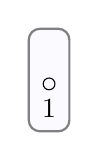
\begin{tikzpicture}
          % 
          \node at (0,0.53) {}; 
          \node at (0,0) [node, label=below:$1$] (1) {};
          % 
          \pgfBox
        \end{tikzpicture} 
      };
%      \node [above=of K1] {$\rho_0$};
      \node [above] at (K1.north) {$\rho_0$};
      \node [right=of K1](R1) {
        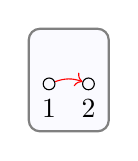
\begin{tikzpicture}
          \node at (0,0.53) {}; 
          \node at (0,0) [node, label=below:$1$] (1) {};
          \node at (.5,0) [node, label=below:$2$] (2) {};
          \draw[coloredge] (1) to[out=20, in=160] (2);
          % 
          \pgfBox
        \end{tikzpicture}
      };
      \path (K1) edge[->] node[trans, above] {} (L1);
      \path (K1) edge[->] node[trans, above] {} (R1);

      \node at (4,2) (L2) {
        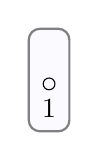
\begin{tikzpicture}
          % 
          \node at (0,0.53) {}; 
          \node at (0,0) [node, label=below:$1$] (1) {} ;
          % 
          \pgfBox
        \end{tikzpicture} 
      };
      \node [right=of L2] (K2) {
        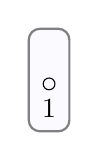
\begin{tikzpicture}
          % 
          \node at (0,0.53) {}; 
          \node at (0,0) [node, label=below:$1$] (1) {};
          % 
          \pgfBox
        \end{tikzpicture} 
      };
%      \node [above=of K2] {$\rho_1$};
            \node [above] at (K2.north) {$\rho_1$};
      \node [right=of K2] (R2) {
        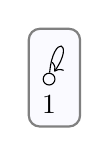
\begin{tikzpicture}
          \node at (0,0) [node, label=below:$1$] (1) {}
          edge [in=55, out=85, loop] ();        
          % 
          \pgfBox
        \end{tikzpicture}
      };
      \path (K2) edge[->] node[trans, above] {} (L2);
      \path (K2) edge[->] node[trans, above] {} (R2);

      \node at (8,2) (L3) {
        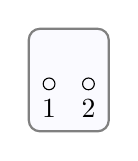
\begin{tikzpicture}
          % 
          \node at (0,0.53) {}; 
          \node at (0,0) [node, label=below:$1$] (1) {} ;
          \node at (0.5,0) [node, label=below:$2$] (2) {} ;
          % 
          \pgfBox
        \end{tikzpicture} 
      };
      \node [right=of L3] (K3) {
        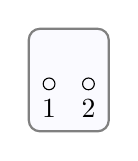
\begin{tikzpicture}
          % 
          \node at (0,0.53) {}; 
          \node at (0,0) [node, label=below:$1$] (1) {} ;
          \node at (0.5,0) [node, label=below:$2$] (2) {} ;
          % 
          \pgfBox
        \end{tikzpicture} 
      };
 %     \node [above=of K3] {$\rho_2$};
      \node [above] at (K3.north) {$\rho_2$};
      \node [right=of K3] (R3) {
        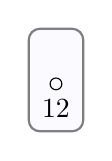
\begin{tikzpicture}
          \node at (0,0.53) {}; 
          \node at (0,0) [node, label=below:$12$] (12) {};
          % 
          \pgfBox
        \end{tikzpicture}
      };
      \path (K3) edge[->] node[trans, above] {} (L3);
      \path (K3) edge[->] node[trans, above] {} (R3);

      %%%%%% second row
      \node at (0,0) (G1) {
        \begin{tikzpicture}
          % 
          \node at (0,0.53) {};
          \node at (0,0) [node, label=below:$1$] (1) {} ;
          % 
          \pgfBox
        \end{tikzpicture} 
      };
      \node [right=of G1] (D1) {
        \begin{tikzpicture}
          % 
          \node at (0,0.53) {}; 
          \node at (0,0) [node, label=below:$1$] (1) {};
          % 
          \pgfBox
        \end{tikzpicture} 
      };
      \node at (3,0) (G2) {
        \begin{tikzpicture}
          % 
          \node at (0,0.53) {}; 
          \node at (0,0) [node, label=below:$1$] (1) {} ;
          \node at (0.5,0) [node, label=below:$2$] (2) {} ;
          \draw[coloredge] (1) to[out=20, in=160] (2);
          % 
          \pgfBox
        \end{tikzpicture} 
      };
      \path (D1) edge[->] node[trans, above] {} (G1);
      \path (D1) edge[->] node[trans, above] {} (G2);
      \path (L1) edge[->] node[trans, above] {} (G1);
      \path (K1) edge[->] node[trans, above] {} (D1);
      \path (R1) edge[->] node[trans, above] {} (G2);

      \node at (5,0) (D2) {
        \begin{tikzpicture}
          % 
          \node at (0,0.53) {};
          \node at (0,0) [node, label=below:$1$] (1) {} ;
          \node at (0.5,0) [node, label=below:$2$] (2) {} ;
          \draw[coloredge] (1) to[out=20, in=160] (2);
          % 
          \pgfBox
        \end{tikzpicture} 
      };
      \node at (7,0) (G3) {
        \begin{tikzpicture}
          % 
          \node at (0,0.53) {}; 
          \node at (0,0) [node, label=below:$1$] (1) {}
          edge [in=55, out=85, loop] ();
          \node at (0.5,0) [node, label=below:$2$] (2) {} ;
          \draw[coloredge] (1) to[out=20, in=160] (2);
          % 
          \pgfBox
        \end{tikzpicture} 
      };

      \path (D2) edge[->] node[trans, above] {} (G2);
      \path (D2) edge[->] node[trans, above] {} (G3);
      \path (L2) edge[->] node[trans, above] {} (G2);
      \path (K2) edge[->] node[trans, above] {} (D2);
      \path (R2) edge[->] node[trans, above] {} (G3);
      
      \node at (9.46,0) (D3) {
        \begin{tikzpicture}
          % 
          \node at (0,0) [node, label=below:$1$] (1) {}
          edge [in=55, out=85, loop] ();
          \node at (0.5,0) [node, label=below:$2$] (2) {} ;
          \draw[coloredge] (1) to[out=20, in=160] (2);
          % 
          \pgfBox
        \end{tikzpicture} 
      };
      \node [right=of D3] (G4) {
        \begin{tikzpicture}
          % 
          \node at (0,0) [node, label=below:$12$] (12) {}
          edge [in=55, out=85, loop] ()
          edge [in=125, out=155, colorloop] ();
          % 
          \pgfBox
        \end{tikzpicture} 
      };
      \node[font=\scriptsize, below] at (G1.south) {$G_0$};
      \node[font=\scriptsize, below] at (D1.south) {$D_0$};      
      \node[font=\scriptsize, below] at (G2.south) {$G_1$};
      \node[font=\scriptsize, below] at (D2.south) {$D_1''$};      
      \node[font=\scriptsize, below] at (G3.south) {$G_2''$};
      \node[font=\scriptsize, below] at (D3.south) {$D_2''$};      
      \node[font=\scriptsize, below] at (G4.south) {$G_3$};      

      \path (D3) edge[->] node[trans, above] {} (G3);
      \path (D3) edge[->] node[trans, above] {} (G4);
      \path (L3) edge[->] node[trans, above] {} (G3);
      \path (K3) edge[->] node[trans, above] {} (D3);
      \path (R3) edge[->] node[trans, above] {} (G4);
    \end{tikzpicture}
  %
\end{center}
%%% Local Variables:
%%% mode: latex
%%% TeX-master: t
%%% End:

		\caption{The derivation $\der{D}'$.}
		\label{fi:derD1}
	\end{figure}
	
	As a consequence, $\der{D}$ and $\der{D}'$ would be switch
	equivalent, but this is not acceptable when viewing equivalence
	classes of derivations as concurrent computations: in $\der{D}$ the
	first two steps are not sequential independent, while in $\der{D}'$
	they are, intuitively because in $\der{D}$ rule $\rho_1$ uses the
	node generated by $\rho_0$ (adding a self-loop to it), while in
	$\der{D}'$ rule $\rho_1$ uses the node that was in the initial
	graph. Also observe that the graphs $G_2$ and $G_2'$ produced after
	two steps in $\der{D}$ and $\der{D'}$ are not isomorphic. From the
	technical point of view, the property of being switch equivalent is
	not closed by prefix, and this prevents deriving a sensible
	concurrent semantics: In fact
	$\der{D} = \dder{D}_0\cdot \dder{D}_1 \cdot \dder{D}_2$ and
	$\der{D}' = \dder{D}_0'\cdot \dder{D}_1' \cdot \dder{D}_2'$ are
	switch equivalent, while if we consider the first two steps,
	derivations $\dder{D}_0 \cdot \dder{D}_1$ and
	$\dder{D}_0' \cdot \dder{D}_1'$ are not switch equivalent.
\end{example} 

Moreover, limiting sequential independence to the case in which the independence
	pair is unique (as suggested in~\cite{baldan2017domains}) brings to the same problems.

For these reasons we believe a theory of rewriting for
left-linear rules in adhesive categories should be developed for
systems where the uniqueness of the independence pair is ensured.

\begin{definition}[Well-switching rewriting systems]
	A left-linear rewriting system $(\X, \R)$ is \emph{well-switching} if it is strong enforcing and, for every derivation $\der{D}:=\{\dder{D}_{i}\}_{i=0}^1$, there is at most one independence pair between $\dder{D}_0$ and $\dder{D}_1$.
\end{definition}


Clearly, linear rewriting systems are well-switching (see Proposition~\ref{pr:weak}).
Moreover, we next observe that various classes of rewriting systems,
comprising all the ones used in modelling the applications to the
encoding of process calculi or of bio and chemical systems mentioned
in the introduction, are actually well-switching.

\subsubsection{Some examples of well-switching rewriting systems}

\todo{Questa sezione è da riscrivere bene}

A first class consists of those rewriting systems over
possibly hierarchical graphical structures obtained as algebras of
suitable signatures where rules are constrained not to merge elements
of top level sorts in the hierarchy (for graphs, nodes can be
merged while edges cannot). The idea here is to consider graph
structures as presheaves on categories in which there are objects that play 
the role of \emph{roots}, i.e.~objects that are not the codomain of 
any arrow besides the identity. 

\begin{definition}[Root-preserving graphical rewriting systems]
	Let $\X$ be a category, an object $X\in \X$ is a \emph{root} if the only arrow with codomain $X$ is $\id{X}$.
	The category $\gph{X}$ of \emph{$\X$-graphs} is the category
	$\Set^{\X}$. A
	\emph{root-preserving graphical rewriting system} is a left-linear
	rewriting system $(\gph{X}, \R)$ such that for each rule
	$(l\colon K\to L, r\colon K\to R)$ in $\R$ it holds
	\begin{enumerate}
		\item for every $X\in \X$ and $x\in L(X)$, there exists a root $Y$
		and an arrow $f\colon Y\to X$ such that $x$ belongs to the image of
		$L(f)\colon L(Y)\to L(X)$;
		\item $r\colon K\to R$ is mono on the roots, i.e.~for every root $X\in \X$ the component $r_X:K(X)\to R(X)$ is injective.
	\end{enumerate}
\end{definition}

For instance, the category $\cat{Graph}$ can be obtained
by taking as $\X$ the category generated by $E \rightrightarrows V$. In this case $E$ is the only root, hence, condition $1$ asks that in the left-hand side of each rule
there are no isolated nodes, while condition $2$ asks that the
morphism $r: K \to R$ is injective on edges, i.e.~it can only merge nodes.

\begin{lemma}{lemma}{lemVTame}
	\label{bono}
	All root-preserving graphical rewriting systems are well-switching.
\end{lemma}

Another interesting class of well-switching rewriting systems is given by e-graphs.

\begin{example}[E-graphs]
	Consider the category $\cat{EGraphs}$, where objects are (directed)
	graphs endowed with an equivalence over nodes, and arrows are graph
	morphisms that preserve the equivalence, as considered
	in~\cite{BaldanGM06}, closely related to e-graphs~\cite{WNW:egg}. 
	Formally, $\cat{EGraphs}$ can be seen as the
	subcategory of the presheaf
	$[E \rightrightarrows V \to Q, \cat{Set}]$ where objects are
	constrained to have the component $V \to Q$ surjective. 
	
	Explicitly, an
	e-graph $G$ is a triple $\langle s_G, t_G, q_G \rangle$ where
	$s_G, t_G: E_G \rightrightarrows V_G$ provides the graphical
	structure, while the surjective function $q_G : V_G \to Q_G$ maps
	each node to the corresponding equivalence class. 
	Notice that the inclusion functor into  $[E \rightrightarrows V \to Q, \cat{Set}]$ 
	creates pullbacks and pushouts \cite{mac2013categories}, so that they are computed component-wise.
	
	A morphism in $\cat{EGraph}$ is mono if the components over $E$
	and $V$ are mono, i.e.~if it is mono as a morphism in
	$\cat{Graph}$. It is regular mono if also the component on
	$Q$ is mono, i.e.~if it reflects equivalence classes besides
	preserving them. This characterisation of regular monos and the fact that pullbacks and pushouts are computed component-wise allows us to prove quasi-adhesivity of $\cat{EGraphs}$ at once. Moreover, one can deduce that every rewriting system $(\X, \R)$ that is left-linear with respect to $\reg(\cat{EGraphs})$ is strong enforcing: this is done exploiting again the inclusion functor into $[E \rightrightarrows V \to Q, \cat{Set}]$.
	
	Left-linear rewriting systems with respect to $\reg(\cat{EGraphs})$ are well-switching. They have been used in~\cite{BaldanGM06} for the graphical implementation of nominal calculi, where,
	differently from~\cite{Gad07}, as a result of name passing the received name is not merged with a local one, but put in the same equivalence class, better tracing the causal dependencies among reductions.
\end{example}


\section{Switch equivalence and concatenable traces}
\todo{intro}


As we mentioned, for linear rewriting systems
it is canonical to identify
derivations that are equal ``up to switching'', i.e.~that differ
only in the order of independent steps. The same notion can be given
for left-linear rewriting systems by relying on the notion of switch.

We  recall some notations on permutations.  A \emph{permutation} on
$\interval[0]{n}$ is a bijection
$\sigma : \interval[0]{n} \to \interval[0]{n}$. It is a
\emph{transposition} $\nu$ if there are $i, j \in \interval{n}$,
$i \neq j$ such that $\sigma(i)=j$, $\sigma(j) = i$, and
$\sigma(k) = k$ otherwise; it is denoted as $\transp{i}[j]$. Given a permutation $\perm$, 
an \emph{inversion} for $\sigma$ is a pair $(i,j)$ such that $i<j$ and
$\sigma(j)< \sigma(i)$; $\inv{\sigma}$ denotes the set of
inversions of $\perm$.

Switch equivalence is now defined as the equivalence relating derivations that 
can be obtained one from another by a sequence of switches. Moreover, intermediate graphs can be taken up to isomorphism according to abstraction equivalence.

\begin{definition}[Switching sequence]
	\label{de:switch-equivalence}
	Let $(\X, \R)$ be a left-linear rewriting system.  Let also
	$\der{D}, \der{E} : G \Mapsto H$ be derivations with the same
	length, $\der{D}=\{\dder{D}_{i}\}_{i=0}^n$ and
	$\der{E}=\{\dder{E}_{i}\}_{i=0}^n$. If
	$\dder{D}_i \cdot \dder{D}_{i+1}$ is a switch of
	$\dder{E}_i \cdot \dder{E}_{i+1}$ for some $i \in [0,n-1]$ and  $\dder{D}_j = \dder{E}_j$ for each $j \not \in \{i,i+1\}$ then we write
	$\der{D} \shift{\transp{i}} \der{E}$. 
	A \emph{switching sequence} is a sequence $\{\der{D}_{k}\}_{k=0}^m$
	of derivations such that
	$\der{D}_0 \shift{\nu_1} \der{D}_1 \shift{\nu_2} \ldots
	\shift{\nu_m} \der{D}_m$  with $\nu_{k} = \transp{i_k}$.
	
	Let us denote by $\nu_{k,h}$ the composition
	$\nu_h \circ \nu_{h-1} \circ \ldots \nu_k$. We say that the
	switching sequence \emph{consists of inversions} if for all
	$k \in \interval[0]{m}$ the transposition $\nu_k$ is an inversion
	for $\nu_{1,m}$.
	
	Two derivations $\der{D}, \der{E}:G\Mapsto H$ are \emph{switch
		equivalent}, written $\der{D}\equiv^{sh} \der{E}$, if there is a
	switching sequence $\{\der{D}_{k}\}_{k=0}^m$ such that
	$\der{D}\equiv_a \der{D}_0 \shift{\nu_1} \der{D}_1 \shift{\nu_2}
	\ldots \shift{\nu_m} \der{D}_m \equiv _a \der{E}$.   
	To point out a chosen permutation of rewriting steps, we will also write $\der{D}\equiv^{sh}_{\sigma} \der{E}$, 
	where $\sigma$ is the composition of the transposition appearing in a chosen switching sequence. 
\end{definition}

\todo{Consistent permutations from switchings}

\subsection{A canonical form for switching sequences} 

As a beginning step in our analysis of switch equivalence, we will establish three lemmas  dealing with derivations of length $3$. 


\begin{lemma}[Forward $3$-steps Lemma]\label{lem:primo}
Let $(\X,\R)$ be a left-linear DPO-rewriting system. Consider a derivation $\der{D}=\{\dder{D}_i\}_{i=0}^2$ and suppose that $(i_0,i_1)$ is a good independence pair between $\dder{D}_0$ and $\dder{D}_1$, $(a_0,a_1)$ one between $\dder{D}_1$ and $\dder{D}_2$ and $(e_0, e_1)$ one between $\dder{D}_0$ and $S_{a_0,a_1}(\dder{D}_2)$.
\end{lemma}
\begin{proof}
	contenuto...
\end{proof}


\begin{lemma}[Backward $3$-steps Lemma]\label{lem:secondo}
	contenuto...
\end{lemma}
\begin{proof}
	contenuto...
\end{proof}



\begin{lemma}[Third $3$-steps Lemma]\label{lem:terzo}
	contenuto...
\end{lemma}
\begin{proof}
	contenuto...
\end{proof}


\todo{dividere in due il lemma dopo. devono venire tre lemmi}
\begin{lemma}[Three steps Lemma]\label{lem:iig1}Let $(\X,\R)$ be a left-linear DPO-rewriting system with $\X$ an $\mathcal{M}$-adhesive category. Consider a derivation $\der{D}=\{\dder{D}_i\}_{i=0}^2$ and suppose that $(i_0,i_1)$ is a good independence pair between $\dder{D}_0$ and $\dder{D}_1$, $(a_0,a_1)$ one between $\dder{D}_1$ and $\dder{D}_2$ and $(e_0, e_1)$ one between $\dder{D}_0$ and $S_{a_0,a_1}(\dder{D}_2)$. Then the following properties hold true.
	\begin{enumerate}
		\item $S_{e_0,e_1}(\dder{D}_0)$ and $S_{a_0,a_1}(\dder{D}_1)$ are weakly sequentially independent.
		\item If $S_{i_0, i_1}(\dder{D}_0)\updownarrow_! \dder{D}_2$ with a good independence pair $(\alpha_0, \alpha_1)$, then  $S_{i_0,i_1}(\dder{D}_1)$ and $S_{\alpha_0, \alpha_1}(\dder{D}_2)$ are weakly sequentially independent.
	\end{enumerate}
	
\end{lemma}
\begin{proof}  As a preliminary step, we are going to use \Cref{def:filler,def:switch} to get some diagrams.  First of all, let $(v,v')$ be the filler between $\dder{D}_0$ and $\dder{D}_1$ associated to $(i_0, i_1)$, then we have
	\[\xymatrix{&&R_0 \ar@/_1cm/[ddrr]_(.35){i_0}|(.7)\hole \ar[dr]^{h_0}&& L_1\ar@/^1cm/[ddll]^(.35){i_1}  \ar[dl]_{m_1}\\&K_0\ar[dr]^{k_0}\ar[dl]_{l_0} \ar@/_.8cm/[ddrr]|(.36)\hole^(.65){v}\ar[ur]^{r_0}&& G_1 && K_1 \ar@/^.8cm/[ddll]|(.36)\hole_(.65){v'}\ar[dl]_{k_1}\ar[lu]_{l_1} \ar[dr]^{r_1}\\L_0 \ar@/_.8cm/[ddrr]_(.2){j_0}|(.31)\hole|(.81)\hole \ar[dr]^(.4){m_0}|(.61)\hole && D_0 \ar[dl]|(.4)\hole_(.65){f_0}\ar[ur]|(.5)\hole^(.7){g_0}&&D_1 \ar[dr]|(.4)\hole^(.65){g_1} \ar[ul]|(.5)\hole_(.65){f_1}&&R_1\ar@/^.8cm/[ddll]^(.2){j_1}|(.31)\hole|(.81)\hole\ar[dl]_{h_1}|(.6)\hole\\&G_0 &&P_1\ar[dr]_{q_1} \ar[dl]^{q_0}\ar[ur]^(.4){p_1}\ar[ul]_(.4){p_0}&&G_2\\L_1 \ar@/^.8cm/[uurr]^(.2){i_1} \ar[ur]_(.35){f_0\circ i_1}|(.61)\hole&&Q_0 \ar[ul]|(.4)\hole_(.65){s_0}\ar[dr]|(.5)\hole^(.65){t_0} &&Q_1\ar[ur]|(.4)\hole^(.65){t_1} \ar[dl]|(.5)\hole_(.65){s_1} && R_0  \ar[ul]^(.35){g_1\circ i_0}|(.61)\hole\ar@/_.8cm/[uull]_(.2){i_0}\\&K_1 \ar[ur]_{q_0\circ v'} \ar[dr]_{r_1} \ar[ul]^{l_1}\ar@/^.8cm/[uurr]_(.65){v'}&&H'_1&& K_0 \ar[ur]_{r_0} \ar[ul]^{q_1\circ v} \ar[dl]^{l_0} \ar@/_.8cm/[uull]^(.65){v}\\&& R_1 \ar[ur]_{\hspace{-5pt}s_1\circ j_1}\ar@/^1cm/[uurr]^(.25){j_1}&& L_0 \ar[ul]^{t_0\circ j_0\hspace{-5pt}} \ar@/_1cm/[uull]_(.25){j_0} |(.69)\hole }\]
	
	Secondly, the filler $(u,u')$ induced by $(a_0, a_1)$ between $\dder{D}_1$ and $\dder{D}_2$ yields:
	\[
	\xymatrix{&&R_1 \ar@/_1cm/[ddrr]_(.35){a_0}|(.7)\hole \ar[dr]^{h_1}&& L_2\ar@/^1cm/[ddll]^(.35){a_1}  \ar[dl]_{m_2}\\&K_1\ar[dr]^{k_1}\ar[dl]_{l_1} \ar@/_.8cm/[ddrr]|(.36)\hole^(.65){u}\ar[ur]^{r_1}&& G_2 && K_2 \ar@/^.8cm/[ddll]|(.36)\hole_(.65){u'}\ar[dl]_{k_2}\ar[lu]_{l_2} \ar[dr]^{r_2}\\L_1 \ar@/_.8cm/[ddrr]_(.2){b_0}|(.31)\hole|(.81)\hole \ar[dr]^(.4){m_1}|(.61)\hole && D_1 \ar[dl]|(.4)\hole_(.65){f_1}\ar[ur]|(.5)\hole^(.7){g_1}&&D_2 \ar[dr]|(.4)\hole^(.65){g_2} \ar[ul]|(.5)\hole_(.65){f_2}&&R_2\ar@/^.8cm/[ddll]^(.2){b_1}|(.31)\hole|(.81)\hole\ar[dl]_{h_2}\\&G_1 &&P_2\ar[dr]_{d_1} \ar[dl]^{d_0}\ar[ur]^(.4){c_1}\ar[ul]_(.4){c_0}&&G_3\\L_2 \ar@/^.8cm/[uurr]^(.2){a_1} \ar[ur]_(.35){f_1\circ a_1}|(.61)\hole&&Q_2 \ar[ul]|(.4)\hole_(.65){x_1}\ar[dr]|(.5)\hole^(.65){y_1} &&Q_3\ar[ur]|(.4)\hole^(.65){y_2} \ar[dl]|(.5)\hole_(.65){x_2} && R_1  \ar[ul]^(.35){g_2\circ a_0}|(.61)\hole\ar@/_.8cm/[uull]_(.2){a_0}\\&K_2 \ar[ur]_{d_0\circ u'} \ar[dr]_{r_2} \ar[ul]^{l_2}\ar@/^.8cm/[uurr]_(.65){u'}&&G'_2&& K_1 \ar[ur]_{r_1} \ar[ul]^{d_1\circ u} \ar[dl]^{l_1} \ar@/_.8cm/[uull]^(.65){u}\\&& R_2 \ar[ur]_{\hspace{-5pt}x_2\circ b_1}\ar@/^1cm/[uurr]^(.25){b_1}&& L_1 \ar[ul]^{y_1\circ b_0\hspace{-5pt}} \ar@/_1cm/[uull]_(.25){b_0} |(.69)\hole }\]


	Finally, the filler $(w,w')$  between $\dder{D}_0$ and $S_{a_0,a_1}(\dder{D}_2)$ given by $(e_0, e_1)$ provides us with:
\[\xymatrix{&&R_0 \ar@/_1cm/[ddrr]_(.35){e_0}|(.7)\hole \ar[dr]^{h_0}&& L_2\ar@/^1cm/[ddll]^(.35){e_1}  \ar[dl]_{f_1\circ a_1}\\&K_0\ar[dr]^{k_0}\ar[dl]_{l_0} \ar@/_.8cm/[ddrr]|(.36)\hole^(.65){w}\ar[ur]^{r_0}&& G_1 && K_2 \ar@/^.8cm/[ddll]|(.36)\hole_(.65){w'}\ar[dl]_{d_0\circ u'\hspace{-5pt}}\ar[lu]_{l_2} \ar[dr]^{r_2}\\L_0 \ar@/_.8cm/[ddrr]_(.2){o_0}|(.31)\hole|(.81)\hole \ar[dr]^(.4){m_0}|(.61)\hole && D_0 \ar[dl]|(.4)\hole_(.65){f_0}\ar[ur]|(.5)\hole^(.7){g_0}&&Q_2 \ar[dr]|(.4)\hole^(.65){y_1} \ar[ul]|(.5)\hole_(.65){x_1}&&R_2\ar@/^.8cm/[ddll]^(.2){o_1}|(.31)\hole|(.81)\hole\ar[dl]_(.35){x_2\circ b_1}\\&G_0 &&P_3\ar[dr]_{n_1} \ar[dl]^{n_0}\ar[ur]^(.4){u_1}\ar[ul]_(.4){u_0}&&G'_2\\L_2 \ar@/^.8cm/[uurr]^(.2){e_1} \ar[ur]_(.35){f_0\circ e_1}|(.61)\hole&&Q_4 \ar[ul]|(.4)\hole_(.65){z_0}\ar[dr]|(.5)\hole^(.65){z'_0} &&Q_5\ar[ur]|(.4)\hole^(.65){z'_1} \ar[dl]|(.5)\hole_(.65){z_1} && R_0  \ar[ul]^(.35){y_1\circ e_0}|(.61)\hole\ar@/_.8cm/[uull]_(.2){e_0}\\&K_2 \ar[ur]_{n_0\circ w'} \ar[dr]_{r_2} \ar[ul]^{l_2}\ar@/^.8cm/[uurr]_(.65){w'}&&G'_1&& K_0 \ar[ur]_{r_0} \ar[ul]^{n_1\circ w} \ar[dl]^{l_0} \ar@/_.8cm/[uull]^(.65){w}\\&& R_2 \ar[ur]_{\hspace{-4pt}z_1\circ o_1}\ar@/^1cm/[uurr]^(.25){o_1}&& L_0 \ar[ul]^{z'_0\circ o_0\hspace{-5pt}} \ar@/_1cm/[uull]_(.25){o_0} |(.69)\hole }\]	
So equipped we can turn to the prove of our claims.	
	\begin{enumerate}
		\item We have to construct the two dotted arrows in the diagram below.
			\[\xymatrix@C=15pt{L_0 \ar[d]_{z'_0\circ o_0}&& K_0 \ar[d]_{n_1\circ w}\ar[ll]_{l_0} \ar[r]^{r_0} & R_0 \ar@{.>}@/^.35cm/[drrr]_(.4){\beta_0}|(.285)\hole \ar[dr]|(.28)\hole_{y_1\circ e_0} && L_1 \ar@{.>}@/_.35cm/[dlll]^(.4){\beta_1} \ar[dl]|(.28)\hole^{y_1\circ b_0}& K_1 \ar[d]^{d_1\circ u}\ar[l]_{l_1} \ar[rr]^{r_1} && R_1 \ar[d]^{g_2\circ a_1}\\G'_1 && \ar[ll]^{z_1} Q_5 \ar[rr]_{z'_1}&& G'_2  && \ar[ll]^{x_2} Q_3 \ar[rr]_{y_2}&& G_3}\]
			
		Consider the arrows $i_0\colon R_0\to D_1$ and $e_0\colon R_0\to Q_2$. An easy computation shows that
			\begin{align*}
				f_1\circ i_0&= h_0\\&=x_1\circ e_0
			\end{align*}
			entailing the existence of  the dotted $\beta'_0\colon R_0\to P_2$ in the diagram
			\[\xymatrix{R_0 \ar@{.>}[dr]^{\beta'_0} \ar@/^.3cm/[drr]^{i_0} \ar@/_.3cm/[ddr]_{e_0}\\ &P_2 \ar[r]^{c_1} \ar[d]_{d_0}& D_1 \ar[d]^{f_1}\\ &Q_2\ar[r]_{x_1} & G_1}\]
			If we define $\beta_0\colon R_0\to Q_3$ as $d_1\circ \beta'_1$, then we easily get that 
		\begin{align*}
			x_2\circ \beta_0&=x_2\circ d_2\circ \beta'_0\\&= y_1\circ d_0\circ \beta'_0\\&=y_1\circ e_0
		\end{align*}
		
		To define $\beta_1$, we proceed similarly. First consider  $i_1\colon L_1\to D_0$ and $b_0\colon L_1 \to Q_2$ and notice that
		\begin{align*}
			g_0\circ i_1&= m_1 \\&= x_1 \circ b_0
		\end{align*}
			implying the existence of $\beta'_1\colon L_1\to P_3$ fitting in the diagram below.
			\[\xymatrix{L_1 \ar@{.>}[dr]^{\beta'_1} \ar@/^.3cm/[drr]^{i_1} \ar@/_.3cm/[ddr]_{b_0}\\ &P_3 \ar[r]^{u_0} \ar[d]_{u_1}& D_0 \ar[d]^{g_0}\\ &Q_2\ar[r]_{x_1} & G_1}\] 
			Let $\beta_1\colon L_1\to Q_5$ be $n_1\circ \beta'_1$, then
			\begin{align*}
				z'_1 \circ \beta_1 & = z'_1 \circ n_1\circ \beta'_1\\&=y_1\circ u_1\circ \beta'_1\\&=y_1\circ b_0
			\end{align*}
		Therefore, $(\beta_0, \beta_1)$ is the wanted independence pair.
			
\item  In addition to the three diagram above, we have a fourth one given by the filler $(\varphi_0, \varphi_1)$ associated to $(\alpha_0, \alpha_1)$. 
\[\xymatrix{&&R_0 \ar@/_1cm/[ddrr]_(.35){\alpha_0}|(.7)\hole \ar[dr]^{g_1\circ i_0}&& L_2\ar@/^1cm/[ddll]^(.35){\alpha_1}  \ar[dl]_{m_2}\\
&K_0\ar[dr]^{\hspace{-4pt}q_1\circ v}\ar[dl]_{l_0} \ar@/_.8cm/[ddrr]|(.36)\hole^(.65){\varphi}\ar[ur]^{r_0}&& G_2 && K_2 \ar@/^.8cm/[ddll]|(.36)\hole_(.65){\varphi'}\ar[dl]_{k_2}\ar[lu]_{l_2} \ar[dr]^{r_2}\\
L_0 \ar@/_.8cm/[ddrr]_(.2){\gamma_0}|(.31)\hole|(.81)\hole \ar[dr]^(.4){\hspace{-4pt}t_0\circ j_0}|(.61)\hole && Q_1 \ar[dl]|(.4)\hole_(.65){s_1}\ar[ur]|(.5)\hole^(.7){t_1}&&D_2 \ar[dr]|(.4)\hole^(.65){g_2} \ar[ul]|(.5)\hole_(.65){f_2}&&R_2\ar@/^.8cm/[ddll]^(.2){\gamma_1}|(.31)\hole|(.81)\hole\ar[dl]_(.35){h_2}\\&H'_1 &&P_4\ar[dr]_{\lambda_1} \ar[dl]^{\lambda_0}\ar[ur]^(.4){\zeta_1}\ar[ul]_(.4){\zeta_0}&&G_3\\
L_2 \ar@/^.8cm/[uurr]^(.2){\alpha_1} \ar[ur]_(.35){s_1\circ \alpha_1}|(.61)\hole&&Q_6 \ar[ul]|(.4)\hole_(.65){\xi_0}\ar[dr]|(.5)\hole^(.65){\xi'_0} &&Q_7\ar[ur]|(.4)\hole^(.65){\xi'_1} \ar[dl]|(.5)\hole_(.65){\xi_1} && R_0  \ar[ul]^(.35){g_2\circ \alpha_0}|(.61)\hole\ar@/_.8cm/[uull]_(.2){\alpha_0}\\&K_2 \ar[ur]_{\lambda_0\circ \phi'} \ar[dr]_{r_2} \ar[ul]^{l_2}\ar@/^.8cm/[uurr]_(.65){\phi'}&&H'_2&& K_0 \ar[ur]_{r_0} \ar[ul]^{\lambda_1\circ \phi} \ar[dl]^{l_0} \ar@/_.8cm/[uull]^(.65){\phi}\\&& R_2 \ar[ur]_{\hspace{-4pt}\xi_1\circ \gamma_1}\ar@/^1cm/[uurr]^(.25){\gamma_1}&& L_0 \ar[ul]^{\xi'_0\circ \gamma_0\hspace{-5pt}} \ar@/_1cm/[uull]_(.25){\gamma_0} |(.69)\hole }\]	

Our aim is to construct the dotted arrow in the following diagram.
		\[\xymatrix@C=15pt{L_1 \ar[d]_{f_0\circ i_0}&& K_1 \ar[d]_{q_0\circ v'}\ar[ll]_{l_1} \ar[r]^{r_1} & R_1 \ar@{.>}@/^.35cm/[drrr]_(.4){\epsilon_0}|(.285)\hole \ar[dr]|(.28)\hole_{s_1\circ j_1} && L_2 \ar@{.>}@/_.35cm/[dlll]^(.4){\epsilon_1} \ar[dl]|(.28)\hole^{s_1\circ \alpha_1}& K_2 \ar[d]^{\lambda_0\circ \phi'}\ar[l]_{l_2} \ar[rr]^{r_2} && R_2 \ar[d]^{\xi_1\circ \gamma_1}\\G_0 && \ar[ll]^{s_0} Q_0 \ar[rr]_{t_0}&& H'_1  && \ar[ll]^{\xi_0} Q_6 \ar[rr]_{\xi'_0}&& H'_2}\]

Let us start considering $j_1\colon R_1\to Q_1$ and $a_0\colon R_1\to D_2$. We have
\begin{align*}
	f_2\circ a_0&=h_1\\&=t_1\circ j_1
\end{align*}
and thus we get an arrow $\epsilon'_0\colon R_1\to P_4$ which makes the diagram below commutative.
			\[\xymatrix{R_1 \ar@{.>}[dr]^{\epsilon'_0} \ar@/^.3cm/[drr]^{j_1} \ar@/_.3cm/[ddr]_{a_0}\\ &P_4 \ar[r]^{\zeta_0} \ar[d]_{\zeta_1}& Q_1 \ar[d]^{t_1}\\ &D_2\ar[r]_{f_2} & G_2}\] 
We can then define $\epsilon_0\colon R_1\to Q_6$ to be $\lambda_0\circ \epsilon'_0$. For such an arrow we have a chain of identities:
\begin{align*}
	\xi_0\circ \epsilon_0&=\xi_0\circ \lambda_0\circ \epsilon'_0\\&=s_1\circ \zeta_0 \circ \epsilon'_0\\&=s_1\circ j_1
\end{align*}

Next, to define $\epsilon_1\colon L_2\to Q_0$ we take $e_1\colon L_2 \to D_0$ and $a_1\colon L_2\to D_1$. By definition we have $	g_0\circ e_1=f_1\circ a_1$, giving us the dotted arrow below
	\[\xymatrix{L_2 \ar@{.>}[dr]^{\epsilon'_1} \ar@/^.3cm/[drr]^{a_1} \ar@/_.3cm/[ddr]_{e_0}\\ &P_1 \ar[r]^{p_1} \ar[d]_{p_0}& D_1 \ar[d]^{f_1}\\ &D_0\ar[r]_{g_0} & G_1}\] 
Now, notice that 
\begin{align*}
	t_1\circ q_1\circ \epsilon'_1&=g_1\circ p_1\circ \epsilon'_1&=g_1\circ a_1\\&=m_2
\end{align*}
Hence $(\alpha_0, q_1\circ \epsilon'_1)$ is an independence pair for $S_{i_0, i_1}(\dder{D}_0)$ and $\dder{D}_2$. By hypothesis $S_{i_0, i_1}(\dder{D}_0)\updownarrow_! \dder{D}_2$ and thus $q_1\circ \epsilon'_1$ must coincide with $\alpha_1$. Now, let $\epsilon_1\colon L_2\to Q_0$ be $q_0\circ \epsilon'_1$. Computing we get
\begin{align*}
t_0\circ \epsilon_1&= t_0\circ q_0\circ \epsilon'_1\\&=s_1\circ q_1\circ \epsilon'_1\\&=s_1\circ \alpha_1
\end{align*}
Allowing us to conclude that  $S_{i_0,i_1}(\dder{D}_1)\updownarrow S_{\alpha_0, \alpha_1}(\dder{D}_2)$.
\qedhere 
			\end{enumerate}
\end{proof}

\subsubsection{Inversions and switch equivalence}
\todo{richiamare cosa sono le inversioni}

\begin{lemma}[Fundamental Lemma] Let $(\der{D}, \alpha, \omega)$ and $(\der{D'}, \alpha, \omega)$ be two decorated derivations and suppose that there exists a non-empty sequence $\{\der{D}_i\}_{i=0}^n$ a of derivations witnessing $\der{D}\equiv^s \der{D}'$. For every $i\in [0,n-1]$, let $\nu_i\colon [0, \lgh(\der{D})-1]\to [0, \lgh(\der{D})-1]$ be the $2$-cycle associated to the switch between $\der{D}_i$ and $\der{D}_{i+1}$, let also $\sigma$ be the associated consistent permutation between $(\der{D}, \alpha, \omega)$ and $(\der{D}', \alpha', \omega')$. Define $k$ as the maximum of the set
\[M_\sigma:=\{j\in [0, \lgh(\der{D}-1] \mid \sigma(j+1) < \sigma(j) \}\]
If every $\nu_i$ is an inversion for $\sigma$, then there exists a family $\{\nu'_i\}_{i=0}^n$ of inversions for $\sigma$ such that jj\todo{capire come scriverlo meglio, l} $\nu'_0=(k, k+1)$.
\end{lemma}
\begin{remark}
	Since $\{\der{D}_i\}_{i=0}^n$ is non-empty, then $\sigma$ must be different from $\id{[0, \lgh(\der{D}-1)]}$ and $M_{\sigma}\neq \emptyset$.
\end{remark}
\begin{proof}
	We proceed by induction on $n$.
	
	\smallskip\noindent $n=1$. In this case there is nothing to prove.
	
	\smallskip \noindent $n>1$. Then...
\end{proof}

\begin{corollary}
	contenuto...
\end{corollary}
\begin{proof}
	contenuto...
\end{proof}


\begin{corollary}
	contenuto...
\end{corollary}
\begin{proof}
	contenuto...
\end{proof}



\begin{corollary}
	contenuto...
\end{corollary}
\begin{proof}
	contenuto...
\end{proof}


\begin{corollary}[No need for useless shifts]
	contenuto...
\end{corollary}
\begin{proof}
	contenuto...
\end{proof}
\newpage


NOTES ON THE FUNDAMENTAL LEMMA WE NEED\todo{da integrare sopra}

Everything is very tame, so that sequential independence coincides with switchability and we do not have ambiguity in the choice of an independence pair


We start with the following situation.
	\[\xymatrix@C=15pt{L_0\ar[d]_{m_0}&& K_0 \ar[d]_{k_0}\ar[ll]_{l_0} \ar[r]^{r_0} & R_0 \ar@/^.35cm/[drrr]_(.4){i_0}|(.285)\hole \ar[dr]|(.28)\hole_{h_0} && L_1 \ar@/_.35cm/[dlll]^(.4){i_1} \ar[dl]|(.28)\hole^{m_1}& K_1 \ar[d]^{k_1}\ar[l]_{l_1} \ar[r]^{r_1} & R_1 \ar[dr]|(.28)\hole_{h_1} \ar@/^.35cm/[drrr]_(.4){j_0}|(.285)\hole  && L_2 \ar@/_.35cm/[dlll]^(.4){j_1} \ar[dl]|(.28)\hole^{m_2}& K_2 \ar[d]^{k_2}\ar[l]_{l_2} \ar[rr]^{r_2} && R_2 \ar[d]^{h_2} \\G_0 && \ar[ll]^{f_0} D_0 \ar[rr]_{g_0}&& G_1  && \ar[ll]^{f_1} D_1 \ar[rr]_{g_1}&& G_2 && \ar[ll]^{f_2} D_2 \ar[rr]_{g_2}&& G_3 }\]
	
	We can do two things:
	
	FIRST SEQUENCE OF SWITCHINGS:
	
	Switch the first two
	

	\[\xymatrix@C=15pt{L_1\ar[d]_{f_0\circ i_1}&& K_1 \ar[d]_{k'_1}\ar[ll]_{l_1} \ar[r]^{r_1} & R_1 \ar@/^.35cm/[drrr]_(.4){a_0}|(.285)\hole \ar[dr]|(.28)\hole_{h'_1} && L_0 \ar@/_.35cm/[dlll]^(.4){a_1} \ar[dl]|(.28)\hole^{m'_0}& K_0 \ar[d]^{k'_0}\ar[l]_{l_0} \ar[r]^{r_0} & R_0 \ar[dr]|(.28)\hole_{g_1\circ j_0} \ar@/^.35cm/[drrr]_(.4){b_0}|(.285)\hole  && L_2 \ar@/_.35cm/[dlll]^(.4){b_1} \ar[dl]|(.28)\hole^{m_2}& K_2 \ar[d]^{k_2}\ar[l]_{l_2} \ar[rr]^{r_2} && R_2 \ar[d]^{h_2} \\G_0 && \ar[ll]^{f'_0} D'_0 \ar[rr]_{g'_0}&& G'_1  && \ar[ll]^{f'_1} D'_1 \ar[rr]_{g'_1}&& G_2 && \ar[ll]^{f_2} D_2 \ar[rr]_{g_2}&& G_3 }\]
	
	Moreover, we know that
	\[m_0=f'_0\circ a_1 \qquad h_1=g'_1\circ a_0\]
	
	Switch second and third 
	\[\xymatrix@C=15pt{L_1\ar[d]_{f_0\circ i_1}&& K_1 \ar[d]_{k'_1}\ar[ll]_{l_1} \ar[r]^{r_1} & R_1 \ar@/^.35cm/[drrr]_(.4){c_0}|(.285)\hole \ar[dr]|(.28)\hole_{h'_1} && L_2 \ar@/_.35cm/[dlll]^(.4){c_1} \ar[dl]|(.28)\hole^{f'_1\circ b_1}& K_2 \ar[d]^{k'_2}\ar[l]_{l_2} \ar[r]^{r_2} & R_2 \ar[dr]|(.28)\hole_{h'_2} \ar@/^.35cm/[drrr]_(.4){d_0}|(.285)\hole  && L_0 \ar@/_.35cm/[dlll]^(.4){d_1} \ar[dl]|(.28)\hole^{\hat{m}_0}& K_0 \ar[d]^{\hat{k}_0}\ar[l]_{l_0} \ar[rr]^{r_0} && R_0 \ar[d]^{g_2\circ b_0} \\G_0 && \ar[ll]^{f'_0} D'_0 \ar[rr]_{g'_0}&& G'_1  && \ar[ll]^{\hat{f}_1} \hat{D}_1 \ar[rr]_{\hat{g}_1}&& G'_2 && \ar[ll]^{f'_2} D'_2 \ar[rr]_{g'_2}&& G_3 }\]
	And we know that
	\[m'_0=\hat{f}_1\circ d_1 \qquad h_2=g'_2\circ d_0\]
	\todo{qua abbiamo usato il secondo lemma dei tre passi (quello condizionale)}Since the rewriting system is very tame and using the three steps lemmas we can characterize $c_0\colon R_1\to \hat{D}_1$ and $c_1\colon L_2\to D'_0$ as the unique arrows fitting in the diagrams
\[\xymatrix@R=15pt@C=15pt{&&R_1 \ar@/_1.2cm/[dddl]_(.4){a_0}|(.63)\hole\ar[dl]^{j_0}\ar[dd]^{c'_0} \ar@{.>}[dr]^{c_0}\\&D_2 \ar[dl]^(.4){f_2}&&\hat{D}_1 \ar[dr]^{\hat{g}_1}\\G_2 && P\ar[dr]_{p_4} \ar[ur]_{p_3}\ar[dl]^{p_1} \ar[ul]^{p_2}&&G'_2\\& D'_1 \ar[ul]^{g'_1}&&D'_2 \ar[ur]_{f'_2}}\]

\[\xymatrix@R=15pt@C=15pt{&&L_2 \ar[dl]^{j_1} \ar@/_1.2cm/[dddl]_(.4){z_1}|(.63)\hole\ar[dd]^{c'_1} \ar@{.>}[dr]^{c_1}\\&D_1 \ar[dl]^(.4){f_1}&&D'_0 \ar[dr]^{g'_0}\\G_1 && Q\ar[dr]_{q_4} \ar[ur]_{q_3}\ar[dl]^{q_1} \ar[ul]_{q_2}&&G'_1\\& D_0 \ar[ul]^{g_0}&&D'_1 \ar[ur]_{f'_1}}\]
	
	
	Switch first and second 
	\[\xymatrix@C=15pt{L_2\ar[d]_{f'_0\circ c_1}&& K_2 \ar[d]_{\hat{k}_2}\ar[ll]_{l_2} \ar[r]^{r_2} & R_2 \ar@/^.35cm/[drrr]_(.4){e_0}|(.285)\hole \ar[dr]|(.28)\hole_{\hat{h}_2} && L_1 \ar@/_.35cm/[dlll]^(.4){e_1} \ar[dl]|(.28)\hole^{\hat{m}_1}& K_1 \ar[d]^{\hat{k}_1}\ar[l]_{l_1} \ar[r]^{r_1} & R_1 \ar@/^.35cm/[drrr]_(.4){t_0} \ar[dr]|(.28)\hole_{\hat{g}_1\circ c_0}   && L_0  \ar[dl]|(.28)\hole^{\hat{m}_0} \ar@/_.35cm/[dlll]^(.4){t_1}& K_0 \ar[d]^{\hat{k}_0}\ar[l]_{l_0} \ar[rr]^{r_0} && R_0 \ar[d]^{g_2\circ b_0} \\G_0 && \ar[ll]^{\hat{f}_0} \hat{D}_0 \ar[rr]_{\hat{g}_0}&& \hat{G}_1  && \ar[ll]^{\tilde{f}_1} \tilde{D}_1 \ar[rr]_{\tilde{g}_1}&& G'_2 && \ar[ll]^{f'_2} D'_2 \ar[rr]_{g'_2}&& G_3 }\]
	Moreover
	\[f_0\circ i_1=\hat{f}_0\circ e_1 \qquad h'_2=\tilde{g}_1\circ e_0\]
	and $(t_0, t_1)$ is characterized using again very tameness and the first $3$-steps Lemma as the unique arrows fitting in:
	\[\xymatrix{&R_1 \ar[dl]_{a_0} \ar@{.>}[dr]^{t_0} \ar@/^.4cm/[dd]|\hole^(.6){c_0}\ar[d]_{t'_0}\\ D'_1 \ar[d]_{g'_1}&P\ar[d]_{p_3} \ar[r]^{p_4} \ar[l]_{p_1}&D'_2\ar[d]^{f'_2}\\G'_1&\hat{D}_1 \ar[l]^{\hat{f}_1}\ar[r]_{\hat{g}_1}& G'_2}\]
	
	
	
	\[\xymatrix@R=15pt@C=15pt{&&L_ 0\ar[dl]^{a_1} \ar@/_1.2cm/[dddl]_(.4){d_1}|(.63)\hole\ar[dd]^{t'_1} \ar@{.>}[dr]^{t_1}\\&D'_0 \ar[dl]^(.4){g'_0}&&\tilde{D}_1 \ar[dr]^{\tilde{f}_1}\\G'_1 && S\ar[dr]_{s_4} \ar[ur]_{s_3}\ar[dl]^{s_1} \ar[ul]_{s_2}&&\hat{G}_1\\& \hat{D}_1 \ar[ul]^{\hat{f}_1}&&\hat{D}_0 \ar[ur]_{\hat{g}_0}}\]
	

	SECOND SEQUENCE OF SWITCHINGS:

	Switch third and second
	
	
	\[\xymatrix@C=15pt{L_0\ar[d]_{m_0}&& K_0 \ar[d]_{k_0}\ar[ll]_{l_0} \ar[r]^{r_0} & R_0 \ar@/^.35cm/[drrr]_(.4){z_0}|(.285)\hole \ar[dr]|(.28)\hole_{h_0} && L_2 \ar@/_.35cm/[dlll]^(.4){z_1} \ar[dl]|(.28)\hole^{f_1\circ j_1}& K_2 \ar[d]^{\check{k}_2}\ar[l]_{l_2} \ar[r]^{r_2} & R_2 \ar[dr]|(.28)\hole_{\check{h}_2} \ar@/^.35cm/[drrr]_(.4){w_0}|(.285)\hole  && L_1 \ar@/_.35cm/[dlll]^(.4){w_1} \ar[dl]|(.28)\hole^{\check{m}_1}& K_1 \ar[d]^{\check{k}_1}\ar[l]_{l_1} \ar[rr]^{r_1} && R_1\ar[d]^{g_2\circ j_0} \\G_0 && \ar[ll]^{f_0} D_0 \ar[rr]_{g_0}&& G_1  && \ar[ll]^{\check{f}_1} \check{D}_1 \ar[rr]_{\check{g}_1}&& \check{G}_2 && \ar[ll]^{\check{f}_2} \check{D}_2 \ar[rr]_{\check{g}_2}&& G_3 }\]
	Moreover
	\[m_1=\check{f}_1\circ w_1 \qquad h_2=\check{g}_2\circ w_0\]
	
	Switch second and first
		\[\xymatrix@C=15pt{L_2\ar[d]_{f_0\circ z_1}&& K_2 \ar[d]_{\mathring{k}_2}\ar[ll]_{l_2} \ar[r]^{r_2} & R_2 \ar@/^.35cm/[drrr]_(.4){y_0}|(.285)\hole \ar[dr]|(.28)\hole_{\mathring{h}_2} && L_0 \ar@/_.35cm/[dlll]^(.4){y_1} \ar[dl]|(.28)\hole^{\check{m}_0}& K_0 \ar[d]^{\check{k}_0}\ar[l]_{l_0} \ar[r]^{r_0} & R_0 \ar[dr]|(.28)\hole_{\check{g}_1\circ z_0} \ar@/^.35cm/[drrr]_(.4){x_0}|(.285)\hole  && L_1 \ar@/_.35cm/[dlll]^(.4){x_1} \ar[dl]|(.28)\hole^{\check{m}_1}& K_1 \ar[d]^{\check{k}_1}\ar[l]_{l_1} \ar[rr]^{r_1} && R_1\ar[d]^{g_2\circ j_0} \\G_0 && \ar[ll]^{\check{f}_0} \check{D}_0 \ar[rr]_{\check{g}_0}&& \check{G}_1  && \ar[ll]^{\mathring{f}_1} \mathring{D}_1 \ar[rr]_{\mathring{g}_1}&& \check{G}_2 && \ar[ll]^{\check{f}_2} \check{D}_2 \ar[rr]_{\check{g}_2}&& G_3 }\]
	As before we have
	\[m_0=\check{f}_0\circ y_1 \qquad \check{h}_2=\mathring{g}_1\circ y_0\]
	The really important thing to notice is that, by very tameness we have
	\begin{align*}
		f_0'\circ c_1&=f'_0\circ q_3\circ c'_1\\&=f_0\circ q_1\circ c'_1\\&=f_0\circ z_1
	\end{align*}
	
	\todo{GOOD! i primi match sono uguali, ora giochiamoci il primo lemma dei tre passi}
	
	Switch second and third
\[\xymatrix@C=15pt{L_2\ar[d]_{f_0\circ z_1}&& K_2 \ar[d]_{\mathring{k}_2}\ar[ll]_{l_2} \ar[r]^{r_2} & R_2 \ar@/^.35cm/[drrr]_(.4){v_0}|(.285)\hole \ar[dr]|(.28)\hole_{\mathring{h}_2} && L_1 \ar@/_.35cm/[dlll]^(.4){v_1} \ar[dl]|(.28)\hole^{\mathring{f}_1 \circ x_1}& K_1 \ar[d]^{\mathring{k}_1}\ar[l]_{l_1} \ar[r]^{r_1} & R_1 \ar@/^.35cm/[drrr]_(.4){u_0}|(.285)\hole\ar[dr]_{\check{h}_1}   && L_0 \ar@/_.35cm/[dlll]^(.4){u_1} \ar[dl]^{\mathring{m}_0}& K_0 \ar[d]^{\mathring{k}_0}\ar[l]_{l_0} \ar[rr]^{r_0} && R_0\ar[d]^{\check{g}_2\circ x_0} \\G_0 && \ar[ll]^{\check{f}_0} \check{D}_0 \ar[rr]_{\check{g}_0}&& \check{G}_1  && \ar[ll]^{\bar{f}_1} \bar{D}_1 \ar[rr]_{\bar{g}_1}&& \bar{G}_2 && \ar[ll]^{\bar{f}_2} \bar{D}_2 \ar[rr]_{\bar{g}_2}&& G_3 }\]

\[\xymatrix@R=15pt@C=15pt{&&R_1 \ar@/_1.2cm/[dddl]_(.4){a_0}|(.63)\hole\ar[dl]^{j_0}\ar[dd]^{c'_0} \ar@{.>}[dr]^{c_0}\\&D_2 \ar[dl]^(.4){f_2}&&\hat{D}_1 \ar[dr]^{\hat{g}_1}\\G_2 && P\ar[dr]_{p_4} \ar[ur]_{p_3}\ar[dl]^{p_1} \ar[ul]^{p_2}&&G'_2\\& D'_1 \ar[ul]^{g'_1}&&D'_2 \ar[ur]_{f'_2}}\]

\[\xymatrix@R=15pt@C=15pt{&&L_1 \ar[dl]^{w_1} \ar@/_1.2cm/[dddl]_(.4){i_1}|(.63)\hole\ar[dd]^{v'_1} \ar@{.>}[dr]^{v_1}\\&\check{D}_1 \ar[dl]^(.4){\check{f}_1}&&\check{D}_0 \ar[dr]^{g'_0}\\G_1 && \check{Q}\ar[dr]_{\check{q}_4} \ar[ur]_{\check{q}_3}\ar[dl]^{\check{q}_1} \ar[ul]_{\check{q}_2}&&\check{G}_1\\& D_0 \ar[ul]^{g_0}&&\mathring{D}_1 \ar[ur]_{\check{f}_1}}\]




HUGE DIAGRAMF


\[\xymatrix@C=15pt{
  & K_1 \ar[d]^{\hat{k}_1}\ar[l]_{l_1} \ar[r]^{r_1} & R_1 \ar@/^.35cm/[drrr]_(.4){t_0} \ar[dr]|(.28)\hole_{\hat{g}_1\circ c_0}   && L_0  \ar[dl]|(.28)\hole^{\hat{m}_0} \ar@/_.35cm/[dlll]^(.4){t_1}& K_0 \ar[d]^{\hat{k}_0}\ar[l]_{l_0} \ar[rr]^{r_0} && R_0 \ar[d]^{g_2\circ b_0} \\G_0 && \ar[ll]^{\hat{f}_0} \hat{D}_0 \ar[rr]_{\hat{g}_0}&& \hat{G}_1  && \ar[ll]^{\tilde{f}_1} \tilde{D}_1 \ar[rr]_{\tilde{g}_1}&& G'_2 && \ar[ll]^{f'_2} D'_2 \ar[rr]_{g'_2}&& G_3 \\
	L_2\ar[d]_{f_0\circ z_1} \ar[u]^{f'_0\circ c_1}&& K_2 \ar[d]_{\mathring{k}_2}\ar[ll]_{l_2} \ar[r]^{r_2} & R_2 \ar@/_.35cm/[urrr]^(.4){e_0}|(.285)\hole \ar[ur]|(.28)\hole^{\hat{h}_2} \ar@/^.35cm/[drrr]_(.4){v_0}|(.285)\hole \ar[dr]|(.28)\hole_{\mathring{h}_2} && L_1 \ar@/^.35cm/[ulll]_(.4){e_1} \ar[ul]|(.28)\hole_{\hat{m}_1} \ar@/_.35cm/[dlll]^(.4){v_1} \ar[dl]|(.28)\hole^{\mathring{f}_1 \circ x_1}& K_1 \ar[d]^{\mathring{k}_1}\ar[l]_{l_1} \ar[r]^{r_1} & R_1 \ar@/^.35cm/[drrr]_(.4){u_0}|(.285)\hole\ar[dr]_{\check{h}_1}   && L_0 \ar@/_.35cm/[dlll]^(.4){u_1} \ar[dl]^{\mathring{m}_0}& K_0 \ar[d]^{\mathring{k}_0}\ar[l]_{l_0} \ar[rr]^{r_0} && R_0\ar[d]^{\check{g}_2\circ x_0} \\G_0 && \ar[ll]^{\check{f}_0} \check{D}_0 \ar[rr]_{\check{g}_0}&& \check{G}_1  && \ar[ll]^{\bar{f}_1} \bar{D}_1 \ar[rr]_{\bar{g}_1}&& \bar{G}_2 && \ar[ll]^{\bar{f}_2} \bar{D}_2 \ar[rr]_{\bar{g}_2}&& G_3 }\]

Now, by determinism we have isomorphisms $\phi_{\check{D}_0}\colon \check{D}_0\to \hat{D}_0$ $\phi_{\check{G}_1}\colon \check{G}_1\to \hat{G}_1$
Notice that
\begin{align*}
	\hat{f}_0\circ \phi_{\check{D}_0}\circ v_1&= \check{f}_0\circ v_1\\&=\check{f}_0\circ \check{q}_3\circ v'_1\\&=f_0\circ \check{q}_1\circ v'_1\\&=f_0\circ i_1\\&=\hat{f}_0\circ e_1
\end{align*}

GOOD: $\phi_{\check{D}_0}$ sends $v_1$ to $e_1$, thus it respects the match of $L_1$. Automatically it sends $v_0$ to $e_0$.

CHECK THAT $\check{g}_2\circ x_0=g_2\circ j_0$

USO IL PRIMO LEMMA DEI TRE PASSI:

	\[\xymatrix{&R_0 \ar[dl]_{i_0} \ar@{.>}[dr]^{x_0} \ar@/^.4cm/[dd]|\hole^(.6){j_0}\ar[d]_{x'_0}\\ D_1 \ar[d]_{g_1}&P'\ar[d]_{p'_3} \ar[r]^{p'_4} \ar[l]_{p'_1}&\check{D}_2\ar[d]^{\check{g}_2}\\G_2&D_2 \ar[l]^{f_2}\ar[r]_{g_2}& G_3}\]



\[\xymatrix@R=15pt@C=15pt{&&L_ 0\ar[dl]^{I_1} \ar@/_1.2cm/[dddl]_(.4){d_1}|(.63)\hole\ar[dd]^{t'_1} \ar@{.>}[dr]^{t_1}\\&D'_0 \ar[dl]^(.4){g'_0}&&\tilde{D}_1 \ar[dr]^{\tilde{f}_1}\\G'_1 && S\ar[dr]_{s_4} \ar[ur]_{s_3}\ar[dl]^{s_1} \ar[ul]_{s_2}&&\hat{G}_1\\& \hat{D}_1 \ar[ul]^{\hat{f}_1}&&\hat{D}_0 \ar[ur]_{\hat{g}_0}}\]

\section{Switch equivalence and concatenable traces}

\begin{lemma}
	\todo{abstract equivalence and switch }
\end{lemma}
\begin{proof}
	contenuto...
\end{proof}
\begin{definition}
	\todo{tracce}
\end{definition}

Before moving forward, we will prove some other useful properties of the switch equivalence relation.

\begin{lemma}
	\todo{lemma 19}
\end{lemma}
\begin{proof}
	contenuto...
\end{proof}


\begin{theorem}
	\todo{preordine}
\end{theorem}
\begin{proof}
	contenuto...
\end{proof}




\section{A class of well-behaved left-linear DPO rewriting systems}


\part{Domains for DPO rewriting}

\chapter{Domains for DPO rewriting}
\section{Weak domains}
\section{From adhesive grammars to weak domains}

\chapter{Conclusions }
\todo{VERY NICE CONCLUSIONS}



\iffalse 
\newpage
QUOZIENTI VARI

The setting from now on is: $\X$ $\mathcal{M}$-adhesive, $(\mathcal{E}, \mathcal{M})$ a proper (maybe also stable) factorization system. $\X$ has all pushouts.

\begin{lemma}\label{lem:pushandpullpb}
	Let $\X$ be a category and suppose that the diagram below is given.
	\[\xymatrix{ P \ar[r]^{p_0} \ar[d]_{p_1}& A  \ar@/^.2cm/[ddr]^{k_0}\ar[d]^{f}\\  B  \ar@/_.2cm/[drr]_{k_1} \ar[r]_g & C \ar[dr]^{h}\\&& D }\]
	Then the following hold true:
	\begin{enumerate}
		\item if the outer boundary is a pullback, then the inner square is a pullback too;
		\item if the inner square is a pullback and $h$ is mono then also the outer square is a pullback.
	\end{enumerate}
\end{lemma}
\begin{proof}\begin{enumerate}
		\item Let $e_0\colon E\to A$ and $e_1\colon E\to B$ be a pair of arrows such that 
		\[f\circ e_0=g\circ e_1\]
		Then we also have 
		\begin{align*}
		k_0\circ e_0 &= h\circ f\circ e_0\\&=h\circ g \circ e_1\\&=k_1\circ e_1
		\end{align*}
		Thus there exists a unique arrow $e\colon E\to P$ such that
		\[p_0\circ e= e_0 \qquad p_1\circ e=e_1\]
		which entails our claim.
		\item We proceed as before considering two arrows $e_0\colon E\to A$ and $e_1\colon E\to B$, but in this case we suppose that 
		\[k_0\circ e_0=k_1\circ e_1\]
		In particular, we have
		\begin{align*}
			h\circ f \circ e_0 &= k_0\circ e_0\\&=k_1\circ e_1\\&=h\circ g\circ e_1
		\end{align*}
		Thus, since $h$ is mono, we can deduce that $f\circ e_0$ and $g\circ e_1$ are equal and the thesis now follows immediately.
		\qedhere 
	\end{enumerate}
	\end{proof} 
	
	
	\begin{lemma}\label{lem:cond} Let $f\colon A\to C$, $g\colon B\to C$ and $h\colon C\to D$ be arrows in a category $\X$, let also $l_0\colon A'\to A$, $l_1\colon B'\to B$ be two monomorphisms. Suppose moreover, that the following squares are pullbacks:
		\[\xymatrix@C=35pt{Q \ar[r]^{q_0} \ar[d]_{q_1} & A' \ar[d]^{h\circ f\circ l_0} & P \ar[r]^{p_0} \ar[d]_{p_1} & A \ar[d]^{f} & Q  \ar[r]^{l_0\circ q_0} \ar[d]_{l_1\circ q_1}& A \ar[d]^{h\circ f}\\ B \ar[r]_{h\circ g\circ l_1} &D& B \ar[r]_{g}& C &  B \ar[r]_{h\circ g} & D}\]
		Then there exists an arrow $\phi\colon P\to Q$ such that $(P, \{q_i\circ \phi\}_{i=0}^1)$ is a pullback for $f\circ l_0$ along $g\circ l_1$.
	\end{lemma} 
	\begin{proof}
To prove the existence of $\phi\colon P\to Q$ it's enough to consider the solid part of the diagram below.
\[\xymatrix@C=30pt{P \ar@{.>}[dr]^{\phi} \ar@/^.2cm/[drr]^{p_0} \ar@/_.2cm/[ddr]_{p_1}\\ & Q  \ar[r]^(.4){l_0\circ q_0} \ar[d]^{l_1\circ q_1}& A \ar[d]^{h\circ f} \\ &B \ar[r]_{h\circ g} & D}\]
Notice that $\phi$ is a monomorphism. If $\phi\circ a=\phi \circ b$ for some $a,b\colon T\rightrightarrows P$ then
\[\begin{split}
	p_0\circ a&=l_0\circ q_0\circ \phi \circ a\\&=l_0\circ q_0\circ \phi \circ b\\&=p_0\circ b
\end{split} \qquad \begin{split}
p_1\circ a&=l_1\circ q_1\circ \phi \circ a\\&=l_1\circ q_1\circ \phi \circ b\\&=p_1\circ b
\end{split} \]

Moreover, we also have the following chain of equalities, showing that  $(P, \{q_i\circ \phi\}_{i=0}^1)$  is a candidate to be a pullback of $f\circ l_0$ along $g\circ l_1$.
\begin{align*}
f\circ l_0\circ q_0\circ \phi &=f\circ p_0\\&=g\circ p_1\\&=g\circ l_1\circ q_1\circ \phi 
\end{align*}
Let now $e_0\colon E\to A'$ and $e_1\colon E\to B'$ be arrows such that 
\[f\circ l_0\circ e_0=g\circ l_1\circ e_1\]
By hypothesis $(P, \{p_i\}_{i=0}^1)$ is a pullback of $f$ along $g$, therefore we there is a unique  arrow $e\colon E\to P$ such that
\[p_0\circ e = l_0\circ e_0 \qquad p_1\circ e=l_1\circ e_1\]
But then the two identities
\[\begin{split}
	l_0\circ q_0\circ \phi\circ e&=p_0\circ e\\& =l_0\circ e_0 \end{split} \qquad \begin{split}l_1\circ q_1\circ \phi\circ e&=p_1\circ e\\& =l_1\circ e_1
\end{split}\]
allow us to conclude that 
\[q_0\circ \phi\circ e=l_0\circ e_0 \qquad q_1\circ \phi\circ e=l_1\circ e_1\]
	
Finally, if $e'\colon E \to P$ is another arrow such that 		
\[q_0\circ \phi\circ e'=l_0\circ e_0 \qquad q_1\circ \phi\circ e'=l_1\circ e_1\]
then we have 
\[q_0\circ \phi\circ e'=q_0\circ \phi\circ e \qquad q_1\circ \phi\circ e'=q_1\circ \phi\circ e\]
Therefore $\phi\circ e'=\phi \circ e$ and we can conclude since $\phi$ is mono.
	\end{proof}


\begin{lemma}
	Da ind pair a pb
\end{lemma}

\begin{proof}
	contenuto...
\end{proof}

\begin{lemma}
	da pb a ind pair
\end{lemma}
\begin{proof}
	contenuto...
\end{proof}

\begin{corollary}
	caratterizzazione
\end{corollary}
\fi 


\bibliographystyle{plain}
\bibliography{bibliog.bib}


\appendix


\chapter{Preliminaries on subobjects, images, pullbacks and factorization systems}\label{app:fact}
This first section is devoted to recall some classic notions related to subobjects, pullbacks and ways to factorize an arrow. The main source for the presentation is \cite[Ch.~1]{dikranjan2013categorical}.

\section{The pullback functor and right $\mathcal{M}$-images}
Let us start defining the \emph{pullback functor} and show how the existence of a left adjoint to it yields a notion of image of an arrow.

\begin{definition}
	Let $\mathcal{M}$ be a class of arrows in a category $\X$ with $\mathcal{M}$-pullbacks. Suppose that $\mathcal{M}$ is stable under pullbacks, then given an arrow $f\colon X\to Y$, we define the \emph{pullback functor} $f^*\colon \mathcal{M}/Y\to \mathcal{M}/X$ sending an arrow $m:M\to Y$ in $\mathcal{M}$ to a chosen pullback of it along $f$. Given a morphism $g:m\to n$ in $\mathcal{M}/Y$, the arrow $f^*(g)$ is the unique one fitting in the diagram below.
	\[\xymatrix{f^*(M)  \ar[dd]_{f^*(m)} \ar@{.>}[dr]_{f^*(g)}\ar[rr]^{p_m}&& M \ar[dr]^{g}\ar[dd]^(.3){m} \\&f^*(N)  \ar[rr]^(.35){p_n}|(.55)\hole \ar[dl]_{f^*(n)}&& N \ar[dl]^{n}\\ X \ar[rr]_{f}&& Y }\]
\end{definition}

\begin{notation}
	If $m\colon M\to X$ is an arrow in $\mathcal{M}$ and $f\colon X\to Y$ is another morphism, we will denote the chosen domain of $f^*(m)$ by $f^*(M)$.
\end{notation}

\begin{proposition} Let $f\colon X\to Y$ be an arrow in a category $\X$ and $\mathcal{M}$ a class of arrows stable under pullbacks and such that $f$ has a pullback along any arrow in $\mathcal{M}$. Let also $F\colon\D\to \mathcal{M}/Y$ be a diagram with a limiting cone $(l, \{l_D\}_{D\in \D})$ and suppose that  $L$ is the domain of $l$. Denoting $F(D)$ by  $m_D\colon M_D\to Y$, if  $(L, \{l_D\}_{D\in \D}+\{l\})$ is limiting for the diagram in $\X$ determined by the family of arrows $\{m_D\}_{D\in \D}$, then for every $f\colon X\to Y$, $f^*$ preserves the limit of $F$.
\end{proposition}
\begin{proof}
	Let $(a, \{a_D\}_{D\in \D})$ be a cocone in $\{\mathcal{M}/X\}$ over $f^*\circ F$. Then we have the solid part of the diagram below.
	\[\xymatrix{A \ar@/_.8cm/[dd]_{a}\ar[d]^{a_D}  \ar@{.>}[r]_-{b} \ar@/^.5cm/@{.>}[rrr]^{c}&f^*(L)  \ar@/^.7cm/[ddl]|(.37)\hole^(.6){f^*(l)} \ar[rr]_{q} \ar[dl]^{f^*(l_D)}&&L \ar@/^.3cm/[ddl]^{l} \ar[dl]_{l_D}\\f^*(M_D)  \ar[d]^{f^*(m_D)} \ar[rr]^(.7){p_{F(D)}}&& M_D \ar[d]_{m_D} \\ X \ar[rr]_{f}&& Y }\]
	
	Now, notice that, for every $D\in \D$ we have
	\begin{align*}
		m_D\circ p_{F(D)} \circ a_D&=f\circ f^*(m_D)\circ a_D \\&=f\circ a
	\end{align*}
	Moreover, given an arrow $g\colon D\to D'$ in $\D$ then we have
	\begin{align*}
		F(g)\circ p_{F(D)}\circ a_D&=p_{F(D')}\circ f^*(F(g))\circ a_D\\&=p_{F(D')}\circ a_{D'}
	\end{align*}
	
	Thus $(A, \{p_{F(D)}\circ a_D\}_{D\in \D}+ \{f\circ a\})$ is a cone over the diagram in $\X$ determined by $\{m_D\}_{D\in \D}$, so that we get the dotted arrow $b\colon A\to L$ in the diagram above. This arrow,  in turn, yields also $a\colon A\to f^*(L)$. Moreover, we also have that
	\[
	\begin{split}
		p_{F(D)}\circ f^*(l_D)\circ b&= l_D\circ q \circ b\\&=l_D\circ c\\&=p_{F(D)}\circ a_D
	\end{split}\qquad 
	\begin{split}
		f^*(m_D) \circ f^*(l_D)\circ b&= f^*(l)\circ b\\&=a\\&=f^*(m_D)\circ a_D
	\end{split}
	\]
	So that $b$ defines an arrow $a\to f^*(l)$ in $\mathcal{M}/X$ auch that $f^*(l_D)\circ b =a_D$
	
	To see that $b$ is unique, let $b'\colon a\to f^*(l)$ be another arrow such that $f^*(l_D)\circ b' =a_D$, then
	\[\begin{split}
		l\circ q \circ b'&=f\circ f^*(l)\circ b'\\&=f\circ a\\&=l\circ c
	\end{split} \qquad \begin{split}
		l_D\circ q \circ b'&=p_{F(D)}\circ f^*(l_D)\circ b'\\&=p_{F(D)}\circ a_D\\&=l_D\circ c
		3\end{split}\]
	Thus $q\circ b'=c$, implying that $b'=b$.
\end{proof}

The previous theorem gives us at once the following result.

\begin{corollary} \label{cor:finlim}
	Let $f\colon X\to Y$ be an arrow in a category $\X$ and $\mathcal{M}$ a class of arrows stable under pullbacks and such that $f$ has a pullback along any arrow in $\mathcal{M}$. Then $f^*$ preserves binary products. If, moreover, $\id{Y}$ belongs to $\mathcal{M}$ then $f^*$ preserves finite products.
\end{corollary}

Having examined the continuity properties of the pullback functor we can now turn to the notion of \emph{right $\mathcal{M}$-images}.

\begin{definition}
	Let $\mathcal{M}$ be a class of arrows in a category $\X$. A \emph{right $\mathcal{M}$-factorization
	} of a morphism $f\colon X\to Y$ is a pair of arrows $m\colon M\to Y$ and $e\colon X\to M$ such that:
	\begin{enumerate}
		\item $m$ belongs to $\mathcal{M}$ and $f=m\circ e$;
		\item given an arrow $n\colon N\to Z$ in $\mathcal{M}$ and two morphisms $g\colon Y\to Z$, $h\colon X\to N$ makint the solid part of the diagram below commutative, then there exists a unique dotted $v\colon M\to N$ fitting in it.
		\[\xymatrix{X \ar[r]_-{e} \ar@/^.4cm/[rr]^{f} \ar[d]_{h}& M \ar[r]_-{m} \ar@{.>}[dl]^{v} & Y \ar[d]^{g}\\N \ar[rr]_{n} && Z}\] 
	\end{enumerate}  
	
	The arrow $m$ will be called the \emph{right $\mathcal{M}$-image} of $f$.
\end{definition}

\begin{remark}\label{rem:uniq}
	Right $\mathcal{M}$-factorization are essentially unique. To see this, let $e\colon X\to M$ and $m\colon M\to Y$ be a right $\mathcal{M}$-factorization of an arrow $f\colon X\to Y$ and suppose that  $e'\colon X\to M'$ and $m'\colon M'\to Y$ is another, then we  get the existence of the dotted arrows in the following two diagrams
	\[\xymatrix{X \ar[r]^-{e}  \ar[d]_-{e'}& M \ar[r]^-{m} \ar@{.>}[dl]^{v} & Y \ar[d]^{\id{Y}} & X \ar[r]^-{e'}  \ar[d]_{e}& M' \ar[r]_-{m'} \ar@{.>}[dl]^{w} & Y \ar[d]^{\id{Y}}\\M' \ar[rr]_{m'} && Y & M \ar[rr]_{m} && Y}\] 
	On the other hand, from the commutativity of the diagram below we get at once that $v\circ w=\id{M'}$ and $w\circ v=\id{M}$.
	\[\xymatrix{X \ar[rr]^-{e}  \ar[dr]_-{e'} \ar[dd]_{e}&& M \ar[r]^-{m} \ar[dl]^{v} & Y \ar[dd]^{\id{Y}} & X \ar[dr]^{e} \ar[rr]^-{e'}  \ar[dd]_{e'}&& M' \ar[r]_-{m'} \ar[dl]^{w} &Y \ar[dd]^{\id{Y}}\\ & M' \ar[dl]^{w}  \ar[drr]^{m'} &&&&M\ar[dl]^{v} \ar[drr]^{m}\\M \ar[rrr]_{m} &&& Y & M' \ar[rrr]_{m'} &&& Y}\] 
\end{remark}


\begin{proposition}\label{prop:im}
	Let $\mathcal{M}$ be a class of arrows in a category $\X$ and suppose that every morphism in $\X$ has a right $\mathcal{M}$-factorization. Then for every arrow $f\colon X\to Y$, there is a functor $f_*\colon \mathcal{M}/X\to \mathcal{M}/Y$ sending $m\colon M\to X$ to a chosen right $\mathcal{M}$-image of $f\circ m$.
\end{proposition}
\begin{notation}
	As in the case of the pullback functor, if $m$ is an arrow $M\to X$, then we will denote the chosen domain of $f_*(m)$ by $f_*(M)$.
\end{notation}
\begin{proof}
	We only have to define $f_*$ on arrows. Let thus $g$ be a morphism in $\mathcal{M}/X$ between $m\colon M\to X$ and $n\colon N\to X$. Now, since \[f\circ m = f\circ n\circ g\] the solid part of the diagram below commutes, allowing us to define $f_*(g)$ as the dotted arrow.
	\[\xymatrix@C=30pt{M \ar[dr]_(.35){m}|(.55)\hole\ar[r]^-{e_m} \ar[d]_{g}& f_*(M)  \ar@/_.3cm/@{.>}[ddl]^(.7){f_*(g)}\ar[r]^-{f_*(m)}& Y \ar[dd]^{\id{Y}}\\N \ar[d]_{e_n} \ar[r]|(.32)\hole^(.6){n} & X  \ar[dr]^{f}\\f_*(N) \ar[rr]_{f_*(n)}&& Y}\]
	
	It is clear that, with the above definition, $f_*(\id{m})=\id{f_*(m)}$. Let $h\colon n\to o$ be another morphism in $\mathcal{M}/X$, then we can build the following diagram.
	\[\xymatrix@C=30pt{M \ar[r]^-{e_m} \ar[d]_{g}& f_*(M)  \ar[d]_{f_*(g)}\ar[r]^-{f_*(m)}& Y \ar[dd]^{\id{Y}}\\N \ar[r]^-{e_n} \ar[d]_{h} & f_*(N) \ar[d]_{f_*(h)} \ar[dr]^{f_*(n)}\\O\ar[r]_-{e_o}& f_*(O) \ar[r]_{f_*(o)}& Y}\]
	From this it follows at once that $f_*(h)\circ f_*(g)=f_*(g\circ h)$.
\end{proof}
\begin{remark} If $\id{X}$ belongs to $\mathcal{M}$, then $f_*(\id{X})$ is a right $\mathcal{M}$-image of $f$.
\end{remark}

The relationship of right $\mathcal{M}$-images to the pullback functors is explained by the following two results.

\begin{proposition}\label{prop:part}
	Let $\mathcal{M}$ be a class of arrows  in a category $\X$, containing  all identities and stable under pullbacks. Suppose, moreover, that every morphism has a right $\mathcal{M}$-factorization. Then $f_*\dashv f^*$ for every arrow $f\colon X\to Y$.  
\end{proposition}
\begin{proof}
	First of all we can notice that for every $m\colon M\to X$ in $\mathcal{M}/X$ the commutativity of the solid part of the following diagram yields the dotted morphism $\eta_n\colon m\to f^*(f_*(m))$.
	\[\xymatrix@C=30pt{M \ar@{.>}[dr]^{\eta_m} \ar@/^.4cm/[drr]^{e_m} \ar@/_.4cm/[ddr]_{m}\\ & f^*(f_*(M)) \ar[d]^{f^*(f_*(m))}\ar[r]^-{p_{f_*(m)}}& f_*(M) \ar[d]^{f_*(m)}\\ & X\ar[r]_f & Y}\]
	
	To see that $\eta_n$ is the component of a unit $\eta\colon \id{\mathcal{M}/X}\to f^*\circ f_*$, let $g$ be a morphism $m\to f^*(n)$ for some $n\colon N\to Y$ in $\mathcal{M}/Y$. If $p_n:f^*(N)\to N$ is the canonical projection, then 
	\begin{align*}
		n\circ p_n\circ g&=f\circ f^*(n)\circ g\\&=f\circ m
	\end{align*}
	Therefore we can consider the diagram below to get $h\colon f_*(m)\to n$ in $\mathcal{M}/Y$. 
	\[\xymatrix@C=30pt{M \ar[r]^-{e_m} \ar[d]_{g}& f_*(M) \ar[r]^-{f_*(m)}\ar@{.>}@/^.3cm/[ddl]^{h} & Y \ar[dd]^{\id{Y}}\\f^*(N) \ar[d]_{p_n}\\N \ar[rr]_{n}&& Y}\]
	
	Finally, the equations
	\[\begin{split}
		f^*(n)\circ f^*(h)\circ \eta_m&=f^*(f_*(m))\circ \eta_m\\&=m\\&=f^*(n)\circ g
	\end{split} \qquad \begin{split}
		p_n\circ f^*(h)\circ \eta_m&=h\circ p_m\circ \eta_m\\&=h\circ e_m\\&=p_n\circ g
	\end{split}\]
	entail that $f^*(h)\circ \eta_m=g$ as wanted.
	
	Let now $h'\colon f_*(m)\to n$ be an arrow such that $f*(h')\circ \eta_m=g$, then
	\begin{align*}
		h'\circ e_m&=h'\circ p_{f_*(m)}\circ \eta_m\\&=p_n\circ f^*(h')\circ \eta_m\\&=p_n\circ g
	\end{align*}
	Thus $h'$ fits in the diagram
	\[\xymatrix@C=30pt{M \ar[r]^-{e_m} \ar[d]_{g}& f_*(M) \ar[r]^-{f_*(m)}\ar@/^.3cm/[ddl]^{h'} & Y \ar[dd]^{\id{Y}}\\f^*(N) \ar[d]_{p_n}\\N \ar[rr]_{n}&& Y}\]
	showing that $h=h'$.	
\end{proof}

\begin{lemma}\label{lem:rfact}
	Let $\mathcal{M}$ be a class of arrows  in a category $\X$, containing all identities then the following are equivalent:
	\begin{enumerate}
		\item $\mathcal{M}$ is stable under pullbacks, $\X$ has all $\mathcal{M}$-pullbacks and every morphism has a right $\mathcal{M}$-factorization;
		\item $\mathcal{M}$ is stable under pullbacks, $\X$ has all $\mathcal{M}$-pullbacks and for every morphism $f\colon X\to Y$, $f^*$ has a left adjoint;
		\item every morphism has a right $\mathcal{M}$-factorization and for every arrow $f\colon X\to Y$, $f_*$ has a right adjoint.
	\end{enumerate}
\end{lemma}
\begin{proof}
	$(1\Rightarrow 2)$ This follows at once from \Cref{prop:part}.
	
	\smallskip \noindent $(2\Rightarrow 1)$ Let $L_f\colon \mathcal{M}/X\to \mathcal{M}/Y$ be the left adjoint to $f^*$. Since $\id{X}$ belongs to $\mathcal{M}$ we can define $m\colon M\to Y$ in $\mathcal{M}$ as  $L_f(\id{X})$. Moreover, let $\eta_{\id{X}}$ be the component at $\id{X}$ of the unit of the adjunction $L_f \dashv f^*$, if $p_m$ is the projection $f^*(M)\to M$, we can also define $e$ as $p_m\circ \eta_{\id{X}}$. Notice that, by construction, $m\circ e=f$.
	\[\xymatrix@C=30pt{X \ar@/^.4cm/[rr]^e \ar@/_.4cm/[dr]_{\id{X}} \ar[r]_-{\eta_{\id{X}}} & f^*(M) \ar[r]_-{p_m} \ar[d]^{f^*(m)}& M \ar[d]^{m}\\ & X \ar[r]_f& Y}\]
	
	We have to show that $e$ and $m$ so defined really give us a right $\mathcal{M}$-factorization of $f$. We thus start with the solid part of the diagram below, with $n\in \mathcal{M}$.
	\[\xymatrix@C=35pt{f^*(M)\ar[dr]^-{p_m}\\X \ar[r]^-{e} \ar[u]^{\eta_{\id{X}}} \ar|(.36)\hole@/_.5cm/[rr]_{f} \ar[d]_{h}&   M \ar[r]^-{m} \ar@{.>}[dl]^(.6){v} & Y \ar[d]^{g}\\N \ar[rr]_{n} && Z}\] 
	
	We can apply the pullback property of the inner rectangle below to get the dotted arrow $w\colon M\to f^*(g^*(N))$, which, by construction, defines an arrow $m\to f^*(g^*(n))$.
	\[\xymatrix@C=30pt{X \ar@/^.5cm/[drrr]^{h} \ar@/_1cm/[ddr]_{\id{X}} \ar@{.>}[dr]^{w}\\ &f^*(g^*(N)) \ar[d]_{f^*(g^*(n))}\ar[r]^-{p_{g^*(n)}}& g^*(N) \ar[d]_{g^*(n)} \ar[r]^{p_n} & N \ar[d]^{n} \\ &X \ar[r]_{f}& Y \ar[r]_g & Z}\]
	
	By construction $w$ defines a morphism $\id{X}\to f^*(g^*(n))$, thus by adjointness, this implies the existence of a unique $\hat{w}\colon m\to g^*(n)$ such that $f^*(\hat{w})\circ \eta_{\id{X}} =w$. Let $v$ be $p_n\circ \hat{w}$, then
	\[\begin{split}
		v\circ e &= p_n\circ \hat{w} \circ p_m\circ \eta_{\id{X}} \\&=p_n\circ p_{g^*(n)}\circ f^*(\hat{w})\circ \eta_{\id{X}}\\&=p_n\circ p_{g^*(n)}\circ w \\&=h
	\end{split}\qquad  \begin{split}
		n\circ v &=n\circ p_n\circ \hat{w}\\&=g\circ g^*(n)\circ \hat{w}\\&=g\circ m\\&
	\end{split}\] 
	
	To see that such $v$ is unique, let $v'$ be another arrow $M\to N$ such that
	\[v'\circ e=h \qquad n\circ v'=g\circ m\]
	The second of these equations entail the existence of the dotted $q\colon M\to g^*(N)$.
	\[\xymatrix{M \ar@{.>}[dr]^{q}\ar@/^.3cm/[drr]^{v'} \ar@/_.3cm/[ddr]_{m}\\ &g^*(N) \ar[d]^{g^*(n)}\ar[r]^{p_n}& N\ar[d]^{n}\\ &Y\ar[r]_{g} & Z}\]
	Notice that, in particular, $q$ is a morphism $m\to g^*(n)$ in $\mathcal{M}/Y$. Now, we can also consider the following diagram, which entails that $f^*(q)\circ \eta_{\id{X}}=w$.
	\[\xymatrix@C=30pt{f^*(M) \ar@/_1.2cm/[ddd]_{f^*(m)}\ar[dd]_{f^*(q)}\ar[rr]^{p_m}&&M \ar[dd]_{q}\ar@/^.9cm/[ddd]_(.4){m}|(.67)\hole \ar@/^.6cm/[ddr]^{v'}\\&X\ar@/^.8cm/[ddl]|(.33)\hole_(.2){\id{X}} \ar[drr]_(.3){h}|\hole|(.74)\hole\ar[ul]^{\eta_{\id{X}}} \ar[ur]_{e}\\ f^*(g^*(N)) \ar[d]^{f^*(g^*(n))}\ar[rr]_(.67){p_{g^*(n)}}&& g^*(N) \ar[d]_{g^*(n)} \ar[r]_(.65){p_n} & N \ar[d]^{n} \\ X \ar[rr]_{f}&& Y \ar[r]_g & Z}\]
	Thus $q$ must coincide with $\hat{w}$ and therefore $v'=v$.
	
	\smallskip \noindent $(1\Rightarrow 3)$ This also follows from \Cref{prop:part}.
	
	\smallskip \noindent $(3\Rightarrow 1)$ Let $R_f\colon \mathcal{M}/Y\to \mathcal{M}/Y$ be the right adjoint to $f_*$. Given $n\colon N\to Y$ in $\mathcal{M}$, we can build the rectangle below, where $f(R_f(n))$ and $e$ is a (chosen) right $\mathcal{M}$-factorization of $f\circ R_f(n)$ and $\epsilon\colon f_*\circ R_f\to \id{\mathcal{M}/Y}$ is the counit of the adjunction $f_* \dashv f^*$. 
	\[\xymatrix{R_f(N) \ar[d]_{R_f(n)} \ar[r]^-{e}& f_*(R_f(N))  \ar[r]^-{\epsilon_n} \ar[dr]_{f_*(R_f(n)) \hspace{3pt}}& N \ar[d]^{n}\\
		X \ar[rr]_{f}&& Y}\]
	
	We have to show that such a rectangle is a pullback. To do so, let $h\colon Z\to N$ and $g\colon Z\to X$ be arrows such that $n\circ h=f\circ g$ and consider the right $\mathcal{M}$-factorization of $g$ given by arrows $i\colon Z\to K$ and $k\colon K\to X$, with $k\in \mathcal{M}$. Thus there exists the dotted $w\colon K\to N$ in the diagram below.
	\[\xymatrix{Z \ar[r]_{i}\ar@/^.4cm/[rr]^{g}\ar[d]_{h}& K \ar@{.>}[dl]^{w} \ar[r]_k & X \ar[d]^{f}\\
		N \ar[rr]_{n}&& Y}\]
	
	In turn, we can factor $f\circ k$ to get the following rectangle and, henceforth, the existence of the dotted $u\colon f_*(K)\to N$.
	\[\xymatrix{K \ar[r]_-{j}\ar@/^.4cm/[rr]^-{f\circ k}\ar[d]_{w}& f_*(K) \ar@{.>}[dl]^{u} \ar[r]_{f_*(k)} & Y \ar[d]^{\id{Y}}\\
		N \ar[rr]_{n}&& Y}\]
	
	By construction $u$ is a morphism $f_*(k)\to n$, we can thus consider the unique morphism $\hat{u}\colon k\to R_f(n)$ such that
	\[\epsilon_n\circ f_*(\hat{u})=u\]
	
	Summing up we have constructed the diagram that follows.
	\[\xymatrix{Z \ar@/^.4cm/[drrrr]^{h}\ar[dr]^{i} \ar@/_1cm/[ddrr]_{g}\\& K \ar[r]^-{\hat{u}} \ar@/_.2cm/[dr]_{k}& R_f(N) \ar[d]_{R_f(n)} \ar[r]^-{e}& f_*(R_f(N))  \ar[r]_-{\epsilon_n} \ar[dr]_{f_*(R_f(n)) \hspace{3pt}}& N \ar[d]^{n}\\ && 
		X \ar[rr]_{f}&& Y}\]
	
	To conclude it is now enough to show that $\hat{u}\circ i$ is the unique morphism $Z\to R_f(N)$ such that 
	\[\epsilon_n\circ e \circ \hat{u}\circ i=h\qquad R_f(n)\circ \hat{u}\circ i=g\]
	
	Let, therefore, $t$ be an arrow $Z\to R_f(N)$ such that
	\[\epsilon_n\circ e \circ t=h\qquad R_f(n)\circ t=g\]
	The second equation provides us with the commutative rectangle below, guaranteeing the existence of the dotted $s\colon k\to R_f(n)$.
	\[\xymatrix{Z \ar[r]_-{i}\ar@/^.4cm/[rr]^-{g}\ar[d]_{t}& K \ar@{.>}[dl]^{s} \ar[r]_{k} & X \ar[d]^{\id{X}}\\
		R_f(N) \ar[rr]_{R_f(n)}&& X}\]
	
	If we compute we get:
	\[\begin{split}
		n\circ \epsilon_n\circ e\circ s&=f_*(R_f(n))\circ e\circ s\\&=f\circ R_f(n)\circ s\\&=f\circ k
	\end{split} \qquad \begin{split}
		\epsilon_n\circ e\circ s\circ i&=\epsilon_n\circ e\circ t\\&=h\\&
	\end{split} \]
	
	On the other hand, the definition of $f_*$ gives us the inner rectangle of the diagram below.
	\[\xymatrix@C=30pt{K \ar@/_1.2cm/[ddd]_{w}\ar[dr]_(.35){k}|(.55)\hole\ar[r]^-{j} \ar[d]_{s}& f_*(K)  \ar@/_.3cm/[ddl]^(.75){f_*(s)}\ar[r]^-{f_*(k)}& Y \ar[dd]^{\id{Y}}\\R_f(N) \ar[d]_{e} \ar[r]|(.34)\hole_(.6){R_f(n)} & X  \ar[dr]^{f}\\f_*(R_f(N)) \ar[d]_{\epsilon_n} \ar[rr]_{f_*(R_f(n))}&& Y\\N\ar@/_.8cm/[urr]_{n}}\]
	
	From the commutativity of the whole diagram it follows that $\epsilon_n\circ f_*(s)=u$ and thus $s=\hat{u}$, entailing the thesis.
\end{proof}

\section{Factorization systems}

We move now to the notion of \emph{factorization system} \cite{adamek2009abstract,bousfield1977constructions,kelly1991note,rosicky2007factorization,tholen1983factorizations}. Let us start by recalling its definition.

\begin{definition}\label{def:fs}
	Let $\X$ be a category and $\mathcal{E}$, $\mathcal{M}$ two classes of arrows, we will say that $(\mathcal{E},\mathcal{M})$ is a \emph{factorization system} if:
	\begin{enumerate}
		\item $\mathcal{E}$ and $\mathcal{M}$ are closed under composition with isomorphisms: if $f\colon X\to Y$ belongs to $\mathcal{E}$ (to $\mathcal{M}$) and $h\colon Y\to Z$ is an isomorphism then $h\circ f$ belongs to $\mathcal{E}$ (to $\mathcal{M}$);
		\item  every arrow $f\colon X\to Y$ of $\X$ admits a \emph{$(\mathcal{E}, \mathcal{M})$-factorization}, i.e.~there are arrows $e\in \mathcal{E}$ and $m\in \mathcal{M}$ with the property that $f=m\circ e$;
		\item every $e\in \mathcal{E}$ has the \emph{left lifting property} with respect to every $m\in \mathcal{M}$: for every commutative square as the one below, with $e\in \mathcal{E}$ and $m\in \mathcal{M}$ there exists a unique dotted $k\colon Y\rightarrow Z$ which fits in it.
		\[\xymatrix{X \ar[r]^g \ar[d]_{e}& Z \ar[d]^{m}\\ Y \ar[r]_{f} \ar@{.>}[ur]^{k}& V}\] 
	\end{enumerate}
	
	A factorization system is \emph{proper} if every $e\in \mathcal{E}$ is epi and every $m\in \mathcal{M}$ is mono; it is \emph{stable} if $\mathcal{E}$ is stable under pullbacks.
\end{definition}

\begin{remark}\label{rem:dual}It is immediate to notice that, given a factorization system $(\mathcal{E}, \mathcal{M})$ on $\X$, then $(\mathcal{M}, \mathcal{E})$ is a factorization system on $\X^{op}$. Such factorization system on $\X^{op}$ is proper if and only if $(\mathcal{E}, \mathcal{M})$ is so, it is stable if and only if $\mathcal{M}$ is stable under pushouts in $\X$.  
\end{remark}

We can now begin to prove some properties of factorization systems.

\begin{proposition}\label{prop:el}
	Let $(\mathcal{E}, \mathcal{M})$ be a factorization system on a category $\X$, then the following hold true:
	\begin{enumerate}
		\item $\mathcal{E}$ is the class of all arrows with the left lifting properties with respect to every $m\in \mathcal{M}$;
		\item every isomorphism belongs to $\mathcal{E}$;
		\item $\mathcal{E}$ is closed under composition.
	\end{enumerate}
\end{proposition}
\begin{proof}
	\begin{enumerate}
		\item By definition, every arrow in $\mathcal{E}$ has the left lifting property with respect to every arrow in $\mathcal{M}$. To prove the converse, let $f\colon X\to Y$ be an arrow with such a property with respect to every element of $\mathcal{M}$.  We can factorize it as $m\circ e$ with $m\colon M\to Y$ in $\mathcal{M}$ and $e\colon X\to M$ in $\mathcal{E}$. Thus, in the diagram below, the outer square commutes and so we get the dotted $k\colon Y\to M$.
		\[\xymatrix{X\ar[d]_f\ar[r]^e & M\ar[d]^{m}\\Y\ar[r]_{\id{Y}} \ar@{.>}[ur]^{k} & Y}\]
		
		On the other hand, $k\circ m$ fits in the diagram below, showing that $k$ and $m$ are mutually inverses. Thus $f=m\circ e$ belongs to $\mathcal{E}$.
		\[\xymatrix{X\ar[rr]^{e} \ar[dd]_{e} \ar[dr]^{f}&& M\ar[dd]^{m} \ar@{<-}[dl]^{m}\\& Y\ar@{<-}[dl]^{k}\\M \ar[rr]_{m}&&Y}\]
		\item By the previous point, it is enough to show that every isomorphism has the left lifting property. But this follows at once: indeed given a square
		\[\xymatrix{X\ar[d]_e\ar[r]^f & M\ar[d]^{m}\\E\ar[r]_{g} \ar@{.>}[ur]^{k} & Y}\]
		the unique $k\colon E\to M$ filling the diagonal in the diagram above is $f\circ e^{-1}$.
		
		\item Let $e\colon X\to Y$ and $e'\colon Y\to Z$ be two arrows in $\mathcal{E}$. Suppose that the outer rectangle below is given, with $m\in \mathcal{M}$.
		\[\xymatrix{X  \ar[r]^f \ar[d]_{e}& M \ar[dd]^{m}\\Y \ar@{.>}[ur]^{k} \ar[d]_{e'}\\Z \ar@{.>}[uur]_{h}\ar[r]_{g}& W}\]
		
		Then the first dotted arrow $k\colon Y\to M$ exists since $e$ has the left lifting property with respecto to $m$. Its existence, in turn yields the existence of the other dotted arrow $h\colon Z\to M$. 
		
		Let $h'\colon Z\to M$ be another arrow such that 
		\[m\circ h'=g \qquad h'\circ e'\circ e=f\]
		Then $h'\circ e'$ must coincide with $k$ by the uniqueness clause of the left lifting property and thus, by the same clause, $h'$ must be equal to $h$. By the first point $e'\circ e$ belongs to $\mathcal{E}$. \qedhere 
	\end{enumerate}
\end{proof}

Taking into account \Cref{rem:dual}, the previous proposition gives us the following results.

\begin{corollary}\label{cor:m}Let $(\mathcal{E}, \mathcal{M})$ be a factorization system on a category $\X$, then the following hold true:
	\begin{enumerate}
		\item every isomorphism belongs to $\mathcal{M}$;
		\item $\mathcal{M}$ is closed under composition.
	\end{enumerate}
\end{corollary}

In the presence of a factorization system, we also have right $\mathcal{M}$-factorizations.

\begin{proposition}\label{prop:rfact}
	Let $(\mathcal{E}, \mathcal{M})$ be a factorization system on a category $\X$. Let $f\colon X\to Y$ be a morphism with $e\colon X\to M$ and $m\colon M\to Y$ as an $(\mathcal{E}, \mathcal{M})$-factorization of $f$, then the pair $(e, m)$ is also a right $\mathcal{M}$-factorization of $f$.
\end{proposition}
\begin{proof}
	Suppose that the solid part of the rectangle below is given, with $n\colon N\to Z$ in $\mathcal{M}$. 
	\[\xymatrix{X \ar[d]_{h} \ar@/^.4cm/[rr]^{f} \ar[r]_{e}& M \ar@{.>}[dl]^{k} \ar[r]_{m} & Y \ar[d]^{g}\\N \ar[rr]_{n}&& Z}\]
	Bu the existence of the dotted $k\colon M\to N$ is guaranteed by the left lifting property of $e$ with respect to $n$.
\end{proof}

The previous proposition, together with \Cref{rem:uniq} gives us the following.

\begin{corollary}\label{prop:iso}
	Let $(\mathcal{E}, \mathcal{M})$ be a factorization system on a category $\X$. If $e\colon Y\to E$, $e'\colon Y\to E'$ and $m\colon Y\to X$, $m'\colon Y'\to X $ are arrows, respectively, in $\mathcal{E}$ and $\mathcal{M}$ such that
	$e'\circ m'=e\circ m$,  then  there exist a unique isomorphism $\phi\colon E \rightarrow E'$ such that the diagram below commutes.
	\[\xymatrix@C=40pt{Y \ar[r]^{e'} \ar[d]_{e}& E' \ar[d]^{m'}\\ E \ar[r]_{m} \ar@{.>}[ur]^{\phi}& X}\]
\end{corollary}

The previous corollary, in turn, allows us to deduce other useful properties of factorization systems.

\begin{proposition}\label{cor:iso} Given a factorization system $(\mathcal{E}, \mathcal{M})$ on a category $\X$, the following hold:
	\begin{enumerate}
		\item an arrow $f\colon X\to Y$ with $(\mathcal{E}, \mathcal{M})$-decomposition given by $e$ in $\mathcal{E}$ and $m\in \mathcal{M}$ is in $\mathcal{M}$ if and only if $e$ is an isomorphism;
		\item $f\in \mathcal{E}$ and $f\in \mathcal{M}$ if and only if $f$ is an isomorphism;
		\item $\mathcal{M}$ is stable under pullback.
		\item  if $(\mathcal{E}, \mathcal{M})$ is proper, then $g\circ f$ is in $\mathcal{M}$ implies $f\in \mathcal{M}$.
	\end{enumerate}
\end{proposition}
\begin{proof}
	\begin{enumerate}
		\item  ($\Rightarrow$) By hypothesis $f=f\circ \id{X}$ is a factorization with $\id{X}\in \mathcal{E}$ and $f\in \mathcal{M}$, thus the thesis follows from \Cref{prop:iso}.
		
		\smallskip \noindent
		($\Leftarrow$) Let $f=m\circ e$ be an $(\mathcal{E}, \mathcal{M})$-factorization. The thesis  follows from \Cref{cor:m} since, if $e$ is an isomorphism, then $f$ is the composition of two arrows in $\mathcal{M}$.
		
		\item This follows from the previous point, \Cref{cor:m} and \Cref{prop:el}.
		
		\item 	Suppose that the square below is a pullback, with $m\in \mathcal{M}$
		\[\xymatrix{X\ar[r]^{g} \ar[d]_{n} & M \ar[d]^{m} \\ Y \ar[r]_{f}  & Z}\] 
		We can factor  $n$ as $t\circ e$ for $e\colon X\to M$ in  $\mathcal{E}$ and $t\colon T\to Y$ in $ \mathcal{M}$.  By the left lifting property we get the dotted $l\colon T\to M$ in the diagram below.
		\[\xymatrix{X \ar[d]_{e}\ar[rr]^{g} & &V\ar[d]^{m}\\  T  \ar@{.>}[urr]^{l} \ar[r]_{t}&Y\ar[r]_{f} & Z}\]
		Therefore we get another diagram
		\[\xymatrix{ T \ar@/^.5cm/[drr]^{l}\ar@{.>}[dr]^{k} \ar@/_.5cm/[ddr]_{t}\\ & X \ar[d]_{n}\ar[r]^{g}& M  \ar[d]^{m} \\ &Y \ar[r]_{f} & Z }\]
		and thus we can deduce the existence of the dotted $k\colon E\to V$. On the one hand, computing we get
		\[\begin{split}
			n\circ 	k\circ e&=t  \circ  e\\ &=n
		\end{split}\qquad \begin{split}
			g\circ k\circ e &=l\circ e\\ &=g \end{split}\]
		and so $k\circ e= \id{X}$.  On the other hand 
		\[\begin{split}
			t\circ k \circ t &= \id{Y} \circ t \\&= t
		\end{split} \qquad 
		\begin{split}
			k \circ t \circ e &= k\circ n \\&= e
		\end{split}
		\]	
		so the following diagram commutes.
		\[
		\xymatrix@C=50pt{X \ar[d]_{e}\ar[r]^{e}& T \ar[d]^{t} \\
			T\ar[ur]^{e\circ k}\ar[r]_{t} & Y}\]
		Hence, by the uniqueness clause of the left lifting property, $e\circ k=\id{E}$. Therefore $e$ is an isomorphism and the thesis follows from  point $1$. 
		
		\item 
		Factor $f$ and $g$ as $m_f\circ e_f$ and $m_g\circ e_g$, respectively. Let also $h$ be $e_g\circ m_f$ and factor it as $m_h\circ e_h$ so that we get 
		\[\xymatrix@C=45pt{& C \ar[dr]^{m_h}&\\
			A\ar[ur]^{e_h} \ar[rr]^{h}  \ar[dr]^{m_f}& &B \ar[d]^{m_g}\\
			X \ar[u]^{e_f} \ar[r]_f& Y \ar[r]_g \ar[ur]^{e_g} & Z}\]
		B \Cref{prop:el,cor:m}, $\mathcal{E}$ and $\mathcal{M}$ are closed under composition, therefore $e_h\circ e_f\in \mathcal{E}$ and $m_g \circ m_h\in \mathcal{M}$. Thus these two arrows gives a $(\mathcal{E}, \mathcal{M})$-factorization of $g\circ f$. On the other hand $g\circ f\in \mathcal{M}$, thus point $1$ above  implies that  $e_h\circ e_f$ is an isomorphism, so $e_f$ is a epic split mono which is also an epimorphism. \qedhere
	\end{enumerate}
\end{proof}

With the help of \Cref{rem:dual} we can easy dualize the previous proposition.
\begin{corollary}\label{cor:iso2}
	Given a factorization system $(\mathcal{E}, \mathcal{M})$ on a category $\X$, the following hold:
	\begin{enumerate}
		\item an arrow $f\colon X\to Y$ is in $\mathcal{E}$ if and only if $m_f$ is an isomorphism;
		\item $\mathcal{E}$ is stable under pushouts;
		\item  if $(\mathcal{E}, \mathcal{M})$ is proper, then $g\circ f$ is in $\mathcal{E}$ implies $g\in \mathcal{E}$.
	\end{enumerate}
\end{corollary}

We conclude this section with a result linking closely factorization systems with the existence of right $\mathcal{M}$-factorizations.

\begin{lemma}\label{lem:fact}Let $\mathcal{M}$ be a class of arrows in a category $\X$ closed under composition with isomorphisms, then the following are equivalent:
	\begin{enumerate}
		\item every arrow $f\colon X\to Y$ has a right $\mathcal{M}$-factorization and $\mathcal{M}$ is closed under composition;
		\item there exists a class $\mathcal{E}$ such that $(\mathcal{E}, \mathcal{M})$ is a factorization system on $\X$.
	\end{enumerate}
\end{lemma}
\begin{proof} $(1\Rightarrow 2)$ Let $\mathcal{E}$ be the class of arrows which have the left lifting property with respect to every element of $\mathcal{M}$. Let us show that the three properties of \Cref{def:fs} hold.
	
	\begin{enumerate}
		\item $\mathcal{M}$ is closed under composition with isomorphisms by hypothesis. On the other hand, if $e\colon X\to Y$ is in $\mathcal{E}$ and $h\colon Y \to Z$ is an isomorphism, then $h\circ e$ still belongs to $\mathcal{E}$. To see this, consider the square below, with $m\in \mathcal{M}$.
		\[\xymatrix{X\ar[r]^{f} \ar[d]_{e}& M\ar[dd]^{m}  \\Y \ar@{.>}[ur]_{k}\ar[d]_h \\Z \ar[r]_{g}& V}\]
		
		The dotted $k\colon Y\to M$ exists, and it is unique, because $e\in \mathcal{E}$. The thesis now follows taking $k\circ h^{-1}$ as the lifting of $g$. 
		
		\item Given $f\colon X\to Y$, let $e\colon X\to M$ and $m\colon M\to Y$ be a right $\mathcal{M}$-factorization of it. We have to show that $e$ belongs to $\mathcal{E}$. We can further factor $e$ as $n\circ d$, with $n\in \mathcal{M}$. Then we can build the rectangle below.
		\[\xymatrix{X  \ar[dr]_(.3){e}\ar[d]_{d} \ar@/^.4cm/[rr]^{f}\ar[r]_{e} & M \ar@{.>}[dl]^(.3){k} \ar[r]_{m} & Y \ar[d]^{\id{Y}}\\
			D \ar[r]_{n} & M \ar[r]_{m}& Y}\]
		
		By hypothesis $m\circ n$ is in $\mathcal{M}$, so we can deduce the existence of the dotted $k\colon M\to D$.   Now, from the diagram below, we can deduce that $n\circ k=\id{M}$.
		\[\xymatrix{X \ar[rr]^{e} \ar[dr]^{d}\ar[dd]_{e}& &M \ar[r]^{m}\ar[dl]^{k}& Y \ar[dd]^{\id{Y}}\\ & D\ar[dl]^{n}\\M\ar[rrr]_{m}&&&Y}\]
		
		On the other hand, the previous result yields also the commutativity of the following diagram, entailing $k\circ n=\id{D}$.
		\[\xymatrix{X \ar[rr]^{d} \ar[dr]^{e}\ar[dd]_{d}& &D \ar[r]^{n}\ar[dl]^{n}& M \ar[dd]^{\id{M}}\\ & M\ar[dl]^{k} \ar[drr]^{\id{M}}\\D\ar[rrr]_{n}&&&M}\]
		
		Now, suppose that the outer square in the diagram below is given, with $v\in \mathcal{M}$.
		\[\xymatrix{X \ar[dd]_{e} \ar[dr]_{d}\ar[rr]^{t}&& V \ar[dd]^{v}\\ & D \ar[dl]^{n} \ar@{.>}[ur]_{h}\\M \ar[rr]_{s}&& Z}\]
		
		Then the dotted $h\colon N\to V$ exists and it is unique since $n$ is a right $\mathcal{M}$-image of  $e$. Thus $h\circ k$ is the unique lifting for $s$ along $v$, proving that $e\in \mathcal{E}$.
		\item This holds by construction.
	\end{enumerate}
	
	\smallskip \noindent $(2\Rightarrow 1)$  This follows from the second point of \Cref{cor:m} and from \Cref{prop:rfact}. \qedhere  
\end{proof}

Putting together \Cref{lem:fact,lem:rfact} we get the following result.

\begin{corollary}\label{cor:fact}
	Let $\mathcal{M}$ be a class of arrows in a category $\X$ closed under composition stable under pullbacks and containing the identities. If $\X$ has $\mathcal{M}$-pullbacks and for every arrow $f\colon X\to Y$ the pullback functor $f^*$ has a left adjoint, then there exists a, unique, class $\mathcal{E}$ such that $(\mathcal{E}, \mathcal{M})$ is a factorization system on $\X$.
\end{corollary}

\subsection{$\mathcal{M}$-subobjects and factorization systems}\label{app:sub}

In this section we focus on studying the category $\mathcal{M}/X$ when $\mathcal{M}$ is a class of monomorphism.

\begin{remark}
	If  $\mathcal{M}$ is a class of monos in a category $\X$, then $\mathcal{M}/X(f,g)$ has cardinality at most one for every two arrows $f$ and $g$ with codomain $X$. Thus it is a preordered class, in which $f\leq g$ if and only if  $\mathcal{M}/X(f,g)$ is non-empty. Now, it is immediate to notice that $f\leq g$ and $g\leq f$, then there exists a (unique) isomorphism fitting in the triangle below.
	\[\xymatrix{A\ar@{.>}[rr]^{\phi} \ar[dr]_{f} && B \ar[dl]^{g}\\ & X}\]
	In such a case we will write $f\equiv g$. It is immediate to see that in this way we get an equivalence relation on the class of objects of $\mathcal{M}/X$.
\end{remark}

Given the previous remark, we are led to the following definition.

\begin{definition} Let $\mathcal{M}$ be a class of monos in a category $\X$. For every object $X$ a \emph{$\mathcal{M}$-subobject} is an equivalence class $[f]$ of an object $f$ in $\mathcal{M}/X$ with respect to $\equiv$. Given two \emph{$\mathcal{M}$-subobjects} $[f]$ and $[g]$, represented by $f$ and $g$, respectively, we will define $[f]\leq [g]$ if and only if $f\leq g$. It is immediate to see that this defines a partially ordered class $(\sub{M}{X}{X}, \leq)$. 
	
	When $\mathcal{M}$ coincides with the class of all monos we will suppress the prefix, so that a \emph{subobject} is just an equivalence class of a mono and $(\msub{X}{X}, \leq)$ will denote the ordered class of such subobjects of $X$.
\end{definition}

\begin{remark}\label{rem:pbo} Let $f\colon X\to Y$ be an arrows admitting a pullback along arrows in $\mathcal{M}/Y$ and suppose that $\mathcal{M}$ is stable under pullbacks. The categories associated to $(\sub{M}{X}{X}, \leq)$ and $(\sub{M}{Y}{Y}, \leq)$ are equivalent to $\mathcal{M}/X$ and $\mathcal{M}/Y$, respectively, thus we get a monotone function $f^{-1}\colon \sub{M}{X}{Y}\to \sub{M}{X}{X}$ sending $[m]$ to $[f^*(m)]$.
	
	Similarly, if $f\circ m$ has a right $\mathcal{M}$-factorization for every $m\in \mathcal{M}$, then the functor $f_*$ induces a monotone function $\exists_f\colon \sub{M}{X}{X}\to \sub{M}{X}{Y}$.
	
	Notice that, whenever $\mathcal{M}$ is stable unr pullbacks, $\X$ has $\mathcal{M}$-pullbacks and  right $\mathcal{M}$-factorizations, then $\exists_f \dashv f^{-1}$ by \Cref{lem:rfact}.
\end{remark}

\Cref{cor:finlim} gives us immediately the following.

\begin{proposition}\label{prop:finlim}
	Let $f\colon X\to Y$ be an arrow in a category $\X$ and $\mathcal{M}$ a class of arrows stable under pullbacks and such that $f$ has a pullback along any arrow in $\mathcal{M}$. Then $f^{-1}$ preserves binary infima. If, moreover, $\id{Y}$ belongs to $\mathcal{M}$ then $f^{-1}$ preserves finite infima.
\end{proposition}

Now, let us recall the following lemma, which is the application of the Adjoint Functor Theorem \cite{freyd1964abelian,freyd1990categories} to the partial ordered case.

\begin{lemma}\label{lem:adj}
	Let $f\colon (P,\leq)\to (Q, \leq)$ be a monotone function. If $f$ preserves all infima then it has a left adjoint.
\end{lemma}
\begin{proof}
	For every $q\in Q$ define
	\[P_q:=\{p\in P \mid q \leq f(p)\}\]
	Clearly if $q'\leq q$ then $P_{q}\subseteq P_{q'}$. Let us define $g(q)$ as the infimum of $P_q$, the previous observation entails that in this way we get a monotone function $g\colon (Q, \leq)\to (P, \leq)$.
	We can also notice that, since $f$ preserves infima:
	\begin{align*}
		f(g(q))&=f(\inf(P_q))\\&=\inf(f(P_q))
	\end{align*}
	Now, by definition, $q$ is less or equal than every element in $f(P_q)$, thus $q\leq f(g(q))$, so that $g(q)$ is actually the infimum of $P_q$. 
	
	So equpped, we can now prove that $g$ is the right adjoint to $f$.
	\begin{itemize}
		\item Suppose that $g(q)\leq p$.  Then $f(g(q))\leq p$, but we already know that $q\leq f(g(q))$, therefore we can conclude that $q\leq f(p)$.
		\item  Suppose that $q\leq f(p)$. Thus $p$ belongs to $P_q$ and so $g(q)\leq p$. \qedhere 
	\end{itemize}
\end{proof}

The previous Lemma, together with \Cref{cor:fact} and \Cref{prop:finlim}, allows us to deduce the following result.

\begin{corollary}\label{cor:fin}
	Let $\mathcal{M}$ be a class of monomorphism in a category $\X$ stable under pullbacks, containing all identities and closed under composition. If $\sub{M}{X}{X}$ is finite for every object $X$ of $\X$, then there exists a factorization system $(\mathcal{E},\mathcal{M})$ on $\X$
\end{corollary}







\chapter{$\mathcal{M}$-adhesive categories}

This first section is devoted to recall the definition and the basic theory of \emph{$\mathcal{M}$-adhesive categories} \cite{azzi2019essence,ehrig2012,ehrig2014adhesive,lack2005adhesive}. 

\begin{notation} 
We stipulate here some notational conventions which will be used throughout this paper. 
\begin{itemize}\item 
	Given a category $\X$ we will not distinguish notationally between $\X$ and its class of objects: so that ``$X\in \X$'' means that $X$ belongs to the class of objects of $\X$.  
	\item 
	If $1$ is a terminal object in a category $\X$,  the unique arrow $X\to 1$ from another object $X$ will be denoted by $!_X$. Similarly, if $0$ is initial in $\X$ then $?_X$ will denote the unique arrow $0\to X$. %When $\X$ is $\Set$ and $1$ is a singleton, $\delta_x$ will denote the arrow $1\to X$ with value $x\in X$.
	\item  $\mor(\X)$, $\mon(\X)$ and $\reg(\X)$ will denote the class of all arrows, monos and regular monos of $\X$, respectively.
	
	\item Given an integer $n\in \mathbb{Z}$, $[0,n]$ will denote the set
	\[[0,n]:=\{x\in \mathbb{N}\mid x\leq n\}\] 
	Indeed, if $n<0$, then $[0,n]=\emptyset$.
\end{itemize}
\end{notation}


\section{The Van Kampen property}
The key property that $\mathcal{M}$-adhesive categories enjoy is given by  the so-called \emph{Van Kampen condition} \cite{brown1997van,johnstone2007quasitoposes,lack2005adhesive}. We will recall it and examine some of its consequences. First of all we need to recall some terminology and facts regarding subclasses of $\mor(\X)$.

\begin{definition}
	Let $\X$ be a category and $\mathcal{A}$ a  subclass of $\mor(\X)$. We say that  $\mathcal{A}$ is
	\begin{itemize}
		\item 
		\emph{stable under pushouts (pullbacks)} if for every pushout (pullbacks) square 
		\[\xymatrix{A\ar[r]^f  \ar[d]_{m}& B \ar[d]^n \\ C \ar[r]_g & D}\]
		if $m \in \mathcal{A}$ ($n\in \mathcal{A}$) then $n \in \mathcal{A}$ ($m \in \mathcal{A}$);
		\item \emph{closed under composition} if $g, f\in \mathcal{A}$ implies $g\circ f\in \mathcal{A}$ whenever $g$ and $f$ are composable;
		\item \emph{closed under decomposition} if $g\circ f, g\in \mathcal{A}$ implies $f\in \mathcal{A}$.
	\end{itemize}
\end{definition}

\begin{remark}In the previous definition, ``decomposition'' corresponds to ``left cancellation'', but we prefer to stick to the name commonly used in literature (see e.g.~\cite{habel2012mathcal}).
\end{remark}


So equipped, we can introduce the notion of \emph{$\mathcal{A}$-Van Kampen square}.
\begin{definition}[Van Kampen property] Let $\X$ be a category  and consider the two diagrams below
	\[\xymatrix@C=10pt@R=10pt{&&&&&A'\ar[dd]|\hole_(.65){a}\ar[rr]^{f'} \ar[dl]_{m'} && B' \ar[dd]^{b} \ar[dl]_{n'} \\ A \ar[dd]_{m}\ar[rr]^{f}&&B\ar[dd]^{n}&&C'  \ar[dd]_{c}\ar[rr]^(.7){g'} & & D' \ar[dd]_(.3){d}\\&&&&&A\ar[rr]|\hole^(.65){f} \ar[dl]^{m} && B \ar[dl]^{n} \\C\ar[rr]_{g} &&D&&C \ar[rr]_{g} & & D}\]
	
	Given  a class of arrows $\mathcal{A}\subseteq \mor(\X)$, we say that the left square \emph{has the Van Kampen property relatively to $\mathcal{A}$}, or that it  is a \emph{$\mathcal{A}$-Van Kampen square} if:
	\begin{enumerate}
		\item is a pushout square;
		\item 	whenever the right cube has pullbacks as back and left faces and the vertical arrows belong to $\mathcal{A}$, then its top face is a pushout if and only if the front and right faces are pullbacks.
	\end{enumerate}
	Pushout squares which enjoy the ``if'' half of the second point of the condition above are called \emph{$\mathcal{A}$-stable}. 
	
We will call a $\mor(\X)$-Van Kampen ($\mor(\X)$-stable) square simply a \emph{Van Kampen} (\emph{stable}) square.
\end{definition}

Before proceeding further, we recall this classical result about pullbacks.

\begin{lemma}\label{lem:pb1}
	Let $\X$ be a category, and consider the following diagram 	in which the right square is a pullback.
	\[\xymatrix{X \ar[d]_{a} \ar[r]^{f}& \ar[r]^{g} Y \ar[d]^{b}& Z \ar[d]^{c}\\ A \ar[r]_{h}& B \ar[r]_{k}& C}\]
	Then the whole rectangle is a pullback if and only if the left square is one.
\end{lemma}

The previous result can be dualised to get an analogous lemma for pushouts.

\begin{lemma}\label{lem:po1}
	Let $\X$ be a category, and consider the following diagram 	in which the left square is a pushout.
	\[\xymatrix{X \ar[d]_{a} \ar[r]^{f}& \ar[r]^{g} Y \ar[d]^{b}& Z \ar[d]^{c}\\ A \ar[r]_{h}& B \ar[r]_{k}& C}\]
	Then the whole rectangle is a pushout if and only if the right square is one.
\end{lemma}

The following proposition establishes a key property of $\mathcal{A}$-Van Kampen squares with a mono as a side: they are not only pushouts, but also pullbacks.
\begin{proposition}\label{prop:pbpo} Let $\mathcal{A}$ be a class of arrows stable under pushouts and containing all the isomorphisms.  If $m\colon A\to C$ is mono and belongs to $\mathcal{A}$, then every $\mathcal{A}$-Van Kampen square
	\[\xymatrix{A\ar[r]^{g} \ar[d]_{m} & B \ar[d]^{n} \\ C \ar[r]_{f}  & D}\]
	is also a pullback square and $n$ is a monomorphism.
\end{proposition}
\begin{proof} We can start considering the cube below and noticing that $n$, being the pushout of $m\in \mathcal{M}$, belongs to $\mathcal{A}$ too.
	\[\xymatrix@C=13pt@R=13pt{&A\ar[dd]|\hole_(.65){\id{A}}\ar[rr]^{g} \ar[dl]_{\id{A}} && B \ar[dd]^{\id{B}} \ar[dl]_{\id{B}} \\ A  \ar[dd]_{m}\ar[rr]^(.65){g} & & B \ar[dd]_(.3){n}\\&A\ar[rr]|\hole^(.65){g} \ar[dl]^{m} && B \ar[dl]^{n} \\C \ar[rr]_{f} & & D}\]
	By construction the top face of the cube is a pushout and the back one a pullback. The left face is a pullback because $m$ is mono. Thus the $\mathcal{A}$-Van Kampen property yields that the front and the right faces are pullbacks. 
\end{proof}

The previous proposition, in turn, allows us to establish the following results.
\begin{lemma}\label{lem:varie}Let $\mathcal{A}$ be a class of arrows stable under pullbacks, pushouts and containing all isomorphisms.  Suppose that, the left square below is $\mathcal{A}$-Van Kampen, while the vertical faces in the right cube are pullbacks.
		\[\xymatrix@C=10pt@R=10pt{&&&&&A'\ar[dd]|\hole_(.65){a}\ar[rr]^{g'} \ar[dl]_{m'} && B' \ar[dd]^{b} \ar[dl]_{n'} \\ A \ar[dd]_{m}\ar[rr]^{g}&&B\ar[dd]^{n}&&C'  \ar@{.>}[dr]_{h} _{}\ar[dd]_{c}\ar[rr]^(.7){f'} & & D' \ar@{.>}[dr]^{k}\ar[dd]_(.3){d}\\&&&&&A\ar[rr]|\hole^(.65){g} \ar[dl]^{m} && B \ar[dl]^{n} \\C\ar[rr]_{f} &&D&&C \ar[rr]_{f} & & D}\]
Supppose, moreover that $m\colon A\to C$ and $d\colon D'\to D$ are mono and that $d$ belongs to $\mathcal{A}$. Then the dotted arrow  $k\colon D'\to B$ exists if and only if the other dotted arrow  $h\colon C'\to A$ exists too.
\end{lemma}

\begin{remark}
	Notice that, since $d$ is a mono and the vertical faces are pullbacks, then $a, b$ and $c$ are monomorphisms too. Moreover, $n$ is mono by \Cref{prop:pbpo}, so that even $m'$ and $n'$ are monos.
\end{remark}

\begin{proof}
	$(\Rightarrow)$ By hypothesis there exists $k:D'\to B$ such that $n\circ k = d$. By \Cref{prop:pbpo}, the bottom face of the cube is a pullback. Thus there exists a unique $h:C'\to A$ as in the diagram below, implying the thesis.
		\[\xymatrix@C=40pt{C'  \ar@{.>}[d]^{h}\ar[r]^{f'} \ar@/_.5cm/[dd]_{c}& D' \ar@/^.5cm/[dd]^{d}\ar[d]_{k}\\ A \ar[d]^{m} \ar[r]^{g} & B \ar[d]_{n} \\  C \ar[r]_f & D}\]
	
	\smallskip \noindent 
	$(\Leftarrow)$ Let $h:C\to A$ be such that $c=m\circ h$. By the $\mathcal{A}$-Van Kampen property the top face of the given cube is a pushout. Thus we get  the dotted $k:D'\to B$ in the following diagram exists.
		\[\xymatrix@C=40pt{A' \ar@/_.5cm/[dd]_{a} \ar[d]^{m'} \ar[r]^{g'} & B' \ar[d]_{n'} \ar@/^.5cm/[dd]^{b} \\  C' \ar[d]^{h} \ar[r]_{f'} & D' \ar@{.>}[d]_{k}\\ A \ar[r]_g& B }\]
Moreover, by construction we have
\[\begin{split}
n\circ k \circ n' &= n\circ b\\&=d\circ n'\\&\\&
\end{split} \qquad \begin{split}
n\circ k \circ f' &= n\circ g\circ h\\&=f\circ m\circ h\\&=f\circ c\\&= d\circ f' \end{split}\]
We can therefore conclude that $n\circ k =d$. \qedhere 
\end{proof}

Finally, we can show that $\mathcal{A}$-stable pushouts enjoy a kind of \emph{pullback-pushout decomposition} property.

\begin{proposition}\label{prop:stab}Let $\X$ be a category and $\mathcal{A}$ a class of arrows stable under pullbacks. Suppose that, in the diagram below, the whole rectangle is an $\mathcal{A}$-stable pushout and the right square a pullback.
	\[\xymatrix{X \ar[d]_{a} \ar[r]^{f}& \ar[r]^{g} Y \ar[d]^{b}& Z \ar[d]^{c}\\ A \ar[r]_{h}& B \ar[r]_{k}& C}\]
	If the arrow $k$ is in $\mathcal{A}$ and it is a monomorphism,  then both squares are pushouts.
\end{proposition}

\begin{proof} We can begin noticing that $g$, being the pullback of $k$, is mono and in $\mathcal{A}$ too. Thus we can build the cube below, in which all the vertical faces are pullbacks, entailing that all the vertical arrows are in $\mathcal{A}$.
	\[\xymatrix@C=20pt@R=10pt{ & &X\ar[dl]_{f} \ar[ddd]^(.333333){\id{X}}|(.666666)\hole\ar[rrr]^{a} &&&A \ar[ddd]^{\id{A}} \ar[dl]^{h}\\& Y\ar[dl]_{\id{Y}} \ar[ddd]|(.333333)\hole_{\id{Y}} &&&B \ar[ddd]^{\id{B}} \ar[dl]_{\id{B}} \\Y \ar[ddd]_{g} \ar[rrr]^{b}&&& B\ar[ddd]^{k}\\&&X \ar[rrr]|(.34)\hole^{a}|(.67)\hole \ar[dl]_{f}&&& A \ar[dl]^{h}\\ & Y  \ar[dl]_{g}&&& B \ar[dl]^{k}\\ Z\ar[rrr]_{c} &&& C}\]
	By hypothesis the face is an $\mathcal{A}$-stable pushout and so its top one is a pushout. Using \Cref{lem:po1} we can conclude that the right half of the rectangle with which we have started is a pushout too. \qedhere 
\end{proof}

\section{$\mathcal{M}$-adhesivity}

In this section we will define the notion of $\mathcal{M}$-adhesivity \cite{azzi2019essence,ehrig2012,ehrig2014adhesive,heindel2009category,lack2005adhesive} and explore some of the consequence of such a property. 

\begin{definition}[$\mathcal{M}$-adhesive category]
	Let $\X$ be a category and consider a subclass $\mathcal{M}$ of the class $\mon(\X)$ of monomorphisms such that:
	\begin{enumerate}
		\item $\mathcal{M}$ contains all isomorphisms and is closed under composition;
		\item $\mathcal{M}$ is stable under pullbacks and pushouts.
	\end{enumerate} 
	We will use $m\colon X\mto Y$ to denote that an arrow $m\colon X\to Y$ belongs to $\mathcal{M}$. $\X$ is said to be \emph{$\mathcal{M}$-adhesive} if
	\begin{enumerate}
		\item for every $m\colon X\mto Y$ in $\mathcal{M}$ and $g\colon Z\to Y$, a pullback square
		\[\xymatrix{P\ar[r]^p \ar@{>->}[d]_{n}& X \ar@{>->}[d]^{m}\\ Z \ar[r]_g& Y}\]
		exists, such pullbacks will be called \emph{$\mathcal{M}$-pullbacks};
		\item for every $m\colon X\mto Y$ in $\mathcal{M}$ and $f\colon X\to Z$, a pushout square
		\[\xymatrix{X \ar[r]^f \ar@{>->}[d]_{m}& Z \ar[d]^{q}\\ Y\ar[r]_p &Q}\]
		exists, such pushouts  will be called \emph{$\mathcal{M}$-pushouts}; 
		\item  $\mathcal{M}$-pushouts are $\mathcal{M}$-Van Kampen squares.
	\end{enumerate}
	
A category $\X$ is said to be \emph{strictly $\mathcal{M}$-adhesive} if $\mathcal{M}$-pushouts are Van Kampen squares.	
\end{definition}

\begin{remark}\label{rem:diff}Our notion of $\mathcal{M}$-adhesivity follows \cite{ehrig2012,ehrig2014adhesive} and is different from the one of \cite{azzi2019essence}. What is called $\mathcal{M}$-adhesivity in that paper corresponds to our strict $\mathcal{M}$-adhesivity. Moreover, in \cite{azzi2019essence} the class $\mathcal{M}$ is assumed to be only stable under pullbacks. However, if $\mathcal{M}$ contains all split monos, then stability under pushouts can be deduced from the other axioms \cite[Prop.~$5.1.21$]{castelnovo2023thesis}.
\end{remark}


\begin{remark}\label{rem:salva} 
	\emph{Adhesivity} and \emph{quasiadhesivity} as defined in \cite{lack2005adhesive,garner2012axioms}  coincide with  strict $\mon(\X) $-adhesivity and strict $\reg(\X)$-adhesivity, respectively. 
\end{remark}

\begin{remark}\label{rem:pb}
	Let $X$ be an object of $\X$, with $\X$ an $\mathcal{M}$-adhesive. category We can consider  the full subcategory $\mathcal{M}/X$ of $\X/X$ made by arrows in $\mathcal{M}$. Since $\X$ has all $\mathcal{M}$-pullbacks, for every arrow $f\colon X\to Y$ we have a functor $f^*\colon \mathcal{M}/Y\to \mathcal{M}/X $ sending $m\colon M \mto X$ to a chosen pullback of it along $f$.
	\end{remark}

A first result we can prove regards closure under decomposition of $\mathcal{M}$.

\begin{proposition}\label{prop:deco}Let  $\mathcal{A}$ be a class of arrows stable under pullbacks. For every arrow $f\colon X\to Y$ and monomorphism $m\colon Y\to Z$, if $m\circ f \in\mathcal{A}$ then $f\in \mathcal{A}$.
\end{proposition}
\begin{proof}Take the diagram
	\[\xymatrix{X \ar[d]_{\id{X}}\ar[r]^{f}& Y \ar[r]^{\id{Y}}  \ar[d]_{\id{Y}}& Y \ar[d]^{m}\\
		X \ar[r]_{f}& Y \ar[r]_{m} & Z}\]
	Since $m$ is mono the right square is a pullback, while the left square is a pullback by construction. By \Cref{lem:pb1} the whole rectangle is a pullback and the thesis follows.
\end{proof}
\begin{corollary}\label{cor:deco}
	In every $\mathcal{M}$-adhesive category $\X$, the class $\mathcal{M}$ is closed under decomposition.
\end{corollary}

Another result which can be immediately established, with the aid of \Cref{prop:pbpo}, is the following one.
\begin{proposition}\label{prop:pbpoad}
	Let $\X$ be an $\mathcal{M}$-adhesive category. Then $\mathcal{M}$-pushouts are also pullback squares.
\end{proposition}

From \Cref{prop:pbpoad}, in turn, we can derive the following corollaries.
\begin{corollary}\label{cor:rego}
	In a $\mathcal{M}$-adhesive category $\X$, every $m\in\mathcal{M}$ is a regular mono.
\end{corollary}
\begin{proof}
Let $m$ be an element of $\mathcal{M}$ and consider its pushout along itself.
\[\xymatrix{X\ar@{>->}[r]^m \ar@{>->}[d]_m& Y\ar@{>->}[d]^{f}\\Y \ar@{>->}[r]_g & Z}\]
By \Cref{prop:pbpoad} this square is a pullback, proving that $m$ is the equalizer of the arrows $f,g\colon Y\rightrightarrows Z$. \qedhere 
\end{proof}

The following result now follows at once noticing that a regular monomorphism which is also epic is automatically an isomorphism.

\begin{corollary}\label{prop:bal}
If $\X$ is an $\mathcal{M}$-adhesive categories, then every epimorphisms in $\mathcal{M}$ is an isomorphisms. In particular, every adhesive category $\X$ is \emph{balanced}: if a morphism is monic and epic, then it is an isomorphism.
\end{corollary}


$\mathcal{M}$-adhesivity is well-behaved with respect to  the comma construction \cite{mac2013categories}, as shown by the following theorem.
\begin{theorem}[\cite{ehrig2006fundamentals,lack2005adhesive}]\label{lem:comma}
	Let $\A$ and $\B$ be respectively an $\mathcal{M}$-adhesive and an $\mathcal{M}'$-adhesive category. Let also $L:\A\rightarrow \C$ be a functor that preserves $\mathcal{M}$-pushouts, and  $R:\B\rightarrow \C$ be a functor which preserves pullbacks.Then $\comma{L}{R}$ is $\cma{M}{M'}$-adhesive, where 
	\[
	\cma{M}{M}':=\{(h,k)\in \mathcal{A}(\comma{L}{R}) \mid h\in \mathcal{M}, k\in \mathcal{M}'\}\]
\end{theorem}

In particular, we can apply this result to slices over and under a given object.

\begin{corollary}\label{cor:slice}
	Let  $X$ be an object of an $\mathcal{M}$-adhesive category $\X$. Then  $\X/X$ and $X/\X$ are, respectively, $\mathcal{M}_X$- and $\mathcal{M}^X$-adhesive, where
	\[\mathcal{M}_X:=\{m\in  \mathcal{A}(\X/X) \mid m\in \mathcal{M} \} \qquad \mathcal{M}^X:=\{m\in  \mathcal{A}(X/\X) \mid m\in \mathcal{M} \}\]
\end{corollary}


Another categorical construction which preserves $\mathcal{M}$-adhesivity property is the formation of the category of functors.

\begin{theorem}[\cite{ehrig2006fundamentals,lack2005adhesive}]\label{thm:functors}
If $\X$ is an $\mathcal{M}$-adhesive category, then for every small category $\Y$, the category $\X^\Y$  of functors $\Y\to \X$ is $\mathcal{M}^{\Y}$-adhesive, where
\[\mathcal{M}^{\Y}:=\{\eta \in \mathcal{A}(\X^\Y) \mid \eta_Y \in \mathcal{M} \text{ for every } Y\in \Y\}\]
\end{theorem}

We can list various examples of $\mathcal{M}$-adhesive categories (see \cite{castelnovo2023thesis,CastelnovoGM22,lack2006toposes}).

\begin{example}\todo{Topos, ipergrafi e grafi}
\end{example}

\begin{example}
	\todo{grafi semplici}
\end{example}


\begin{example}\todo{GRAFI GERARCHICI}
\end{example}

\begin{example}\todo{term graph}
\end{example}

We end this section proving a useful property of $\mathcal{M}$-adhesive categories:  $\mathcal{M}$-pushout-pullback decomposition.


\begin{lemma}[$\mathcal{M}$-pushout-pullback decomposition]\label{lem:popb} Let $\X$ be an $\mathcal{M}$-adhesive category  and suppose that, in the diagram below, the whole rectangle is a pushout and the right square a pullback.
\[\xymatrix{X \ar[d]_{a} \ar[r]^{f}& \ar[r]^{g} Y \ar[d]^{b}& Z \ar[d]^{c}\\ A \ar[r]_{h}& B \ar[r]_{k}& C}\]
	Then the following statements hold true:
	\begin{enumerate}
\item if $a$ belongs to $\mathcal{M}$ and $k$ is a monomorphism,  then both squares are pushouts and pullbacks;
\item if $f$ and $k $ are in  $\mathcal{M}$, then both squares are pushouts and pullbacks.
	\end{enumerate}
\end{lemma}
\begin{proof}
\begin{enumerate}
	\item By \Cref{prop:stab}, it follows that both squares are pushouts, thus the thesis follows from \Cref{prop:pbpoad}.
	\item By hypothesis, $g$ is the pullback of an arrow in $\mathcal{M}$, thus it belongs to it. But then $g\circ f\in \mathcal{M}$ too  and the whole rectangle is a $\mathcal{M}$-pushout. Therefore, by \Cref{prop:pbpoad} a pullback, so that its left half is a pullback too, by \Cref{prop:pbpo}. Moreover $k\circ h$ is in $\mathcal{M}$ as the pushout of $g\circ f$ and, by \Cref{cor:deco}, we also know that $h\in \mathcal{M}$.  
	
	Using \Cref{lem:po1}, it is enough to show that the left half of the original rectangle is a pushout. We can build the following cube:
	\[\xymatrix@C=20pt@R=10pt{ & &X\ar@{>->}[dl]_{f} \ar[ddd]^(.333333){\id{X}}|(.666666)\hole\ar[rrr]^{a} &&&A \ar[ddd]^{\id{A}} \ar@{>->}[dl]^{h}\\& Y\ar[dl]_{\id{Y}} \ar[ddd]|(.333333)\hole_{\id{Y}} &&&B \ar[ddd]^{\id{B}} \ar[dl]_{\id{B}} \\Y \ar@{>->}[ddd]_{g} \ar[rrr]^{b}&&& B\ar@{>->}[ddd]^{k}\\&&X \ar[rrr]|(.34)\hole^{a}|(.67)\hole \ar@{>->}[dl]_{f}&&& A \ar@{>->}[dl]^{h}\\ & Y \ar[rrr]|(.67)\hole^{b} \ar@{>->}[dl]_{g}&&& B \ar@{>->}[dl]^{k}\\ Z\ar[rrr]_{c} &&& C}\]
	Its vertical faces are all pullbacks and all the vertical arrows are in $\mathcal{M}$, hence the top face is a pushout and we can conclude. \qedhere 
\end{enumerate}
\end{proof}

\subsection{Pushout complements}

We turn now to the exam of the notion of \emph{pushout complement}. We will prove that, in an $\mathcal{M}$-adhesive category $\X$ certain pushout complements are unique and are \emph{final pullbacks complements} in the sense of \cite{dyckhoff1987exponentiable,corradini2006sesqui}.

\begin{definition}[Pushout complement]
Let $f\colon X\to Y$ and $g\colon Y\to Z$ be two composable arrows in a category $\X$. A \emph{pushout complement} for the composable pair $(f,g)$ is a pair $(h,k)$ with $h\colon X\to W$ and $k\colon W\to Z$ such that the square below commutes and it is a pushout.
\[\xymatrix{X \ar[r]^{f} \ar[d]_{h}& Y \ar[d]^{g} \\ W \ar[r]_{k}& Z}\]
\end{definition}

\begin{example}
	In a generic category $\X$, pushout complements may not exist: in $\Set$ the arrows $?_{2}\colon \emptyset \to 2$ and $!_2\colon 2\to 1$ do not have a pushout complement.
	
	Moreover, composable arrows $f\colon X\to Y$ and $g\colon Y\to Z$ may have  pushout complements which are non-isomorphic: for instance, in $\Set$ the two squares below are both pushouts.
	
	\[\xymatrix{2 \ar[r]^{!_2} \ar[d]_{\id{2}}& 1 \ar[d]^{\id{1}} & 2 \ar[r]^{!_2} \ar[d]_{!_2}& 1 \ar[d]^{\id{1}}\\ 2 \ar[r]_{!_2}& 1 & 1 \ar[r]_{\id{1}}& 1}\]
\end{example}


In an $\mathcal{M}$-adhesive category we can approach pushout complements in a more abstract way, using the pullback functor of \Cref{rem:pb}.

\begin{definition}
Let $F\colon \X \to \Y$ be a functor and $Y$ an object of $\Y$. We say that $F$ has a \emph{partial right adjoint at $Y$} if there exists an object $G(Y)$ in $\X$ and an arrow $\epsilon_Y\colon F(G(Y))\to Y$ such that, for every  $f\colon F(X)\to Y$ there exists a unique $g\colon X\to G(Y)$ making the diagram below commutative.
\[\xymatrix@C=15pt{F(X) \ar[rr]^{F(g)} \ar[dr]_{f}&&F(G(Y)) \ar[dl]^{\epsilon_Y}\\ & Y}\]
\end{definition} 

\begin{remark}
	It is immediate to see that $F$ is a left adjoint if and only if it has a partial right adjoint at every $Y\in \Y$.
\end{remark}

We can prove two  useful properties of partial right adjoints.

\begin{proposition}\label{prop:uni}
	Let $F\colon \X\to \Y$ be a functor and suppose that it has a partial right adjoint $(G(Y), \epsilon_Y)$ at $Y$. Then the following hold true:
	\begin{enumerate}
\item there is a natural isomorphism $\psi\colon \X(-, G(Y))\to \Y(F(-), Y)$;
\item if $(G'(Y), \epsilon'_Y)$ is another partial right adjoint to $F$ at $Y$, then there exists a unique isomorphism $\phi_Y\colon G(Y)\to G'(Y)$ such that the diagram below commutes.
\[\xymatrix@C=15pt{F(G(Y)) \ar[rr]^{F(\phi_Y)} \ar[dr]_{\epsilon_Y} & &F(G'(Y)) \ar[dl]^{\epsilon'_Y}\\ & Y}\]
	\end{enumerate}
\end{proposition}
\begin{proof}
	\begin{enumerate}
		\item Given an object $X$ of $\X$ we can define $\phi_X$ putting
		\begin{align*}
			\phi_X \colon \X(X, G(Y))&\to \Y(F(X), Y)\\
			g&\mapsto \epsilon_Y\circ F(g)
		\end{align*}
		By definition of partial right adjoint $\phi_X$ is a bijection. Consider now an arrow $f\colon X_1\to X_2$, then, for every $g\colon X_2\to G(Y)$ we have:
		\begin{align*}
			\phi_X(g)\circ F(f)&=\epsilon_Y\circ F(g)\circ F(f)\\&= \epsilon_Y\circ F(g\circ f)\\&=\phi_X(g\circ f)
		\end{align*}
		Naturality now follows at once.
		
		\item Let $\phi_Y\colon G(Y)\to G'(Y)$ and $\phi'_Y\colon G(Y)\to G'(Y)$ be the unique arrows making the diagram below commutative.
\[\xymatrix@C=15pt{F(G(Y)) \ar[rr]^{F(\phi_Y)} \ar[dr]_{\epsilon_Y} & &F(G'(Y)) \ar[dl]^{\epsilon'_Y} && F(G'(Y)) \ar[rr]^{F(\phi_Y)} \ar[dr]_{\epsilon'_Y} & &F(G(Y)) \ar[dl]^{\epsilon_Y}\\ & Y &&&&Y}\]
		Now, we can notice that the diagram belows commute.
	
	\[\xymatrix{F(G(Y)) \ar[r]^{F(\phi_Y)} \ar[dr]_{\epsilon_Y} &F(G'(Y)) \ar[r]^{F(\phi_Y)} \ar[d]_{\epsilon'_Y} & F(G(Y)) \ar[dl]^{\epsilon_Y} \\ & Y \\ F(G'(Y)) \ar[r]_{F(\phi'_Y)} \ar[ur]^{\epsilon'_Y} &F(G(Y)) \ar[r]_{F(\phi'_Y)} \ar[u]_{\epsilon_Y} & F(G'(Y)) \ar[ul]_{\epsilon'_Y}}\]	
This implies at once that $\phi_Y$ and $\phi'_Y$ are mutally inverse. \qedhere 
	\end{enumerate}
	
\end{proof}

\begin{lemma}\label{lem:part}
	Let $\X$ be an  an $\mathcal{M}$-adhesive category  and cosinder a pair $(m,f)$ with $m\colon M\mto X $ in $\mathcal{M}$ and $f:X\to Y$. If $(h, k)$ is a pushout complement for the pair $(m,f)$, then there exists an isomorphism $\epsilon_k:f^*(k)\to m$ in $\mathcal{M}/X$ such that $(k, \epsilon_k)$ is  a partial right adjoint at $m$ to the pullback functor $f^*\colon \mathcal{M}/Y\to \mathcal{M}/X$.
\end{lemma}
\begin{proof}
	By \Cref{prop:pbpoad}, in the diagram below the inner square is both  a pushout and a pullback, yielding the dotted isomorphism $\epsilon_k\colon f^*(Q)\to M$.
\[\xymatrix{f^*(Q) \ar@{.>}[dr]^{\epsilon_k} \ar@{>->}@/^.3cm/[drr]^{f^*(k)} \ar@/_.3cm/[ddr]_{p}\\& M \ar@{>->}[r]^{m}\ar[d]_{h}& X \ar[d]^f \\&Q\ar@{>->}[r]_{k}&Y}\]

To see that in this way we get a partial right adjoint, let $g\colon f^*(n)\to m $ be a morphism in $\mathcal{M}/X$, then we have the solid diagram below
\[\xymatrix{f^*(N) \ar[dr]^{g} \ar@{>->}@/^.3cm/[drr]^{f^*(n)} \ar[ddd]_{q}\\& M \ar@{>->}[r]^{m}\ar[d]_{h}& X \ar[d]^f \\&Q\ar@{>->}[r]_{k}&Y\\N \ar@{>->}@/_.3cm/[urr]_{n} \ar@{.>}[ur]^{t}}\]
Now, since $n$ and $f^*(n)$ are in $\mathcal{M}$ we can form two other pullback squares:
\[\xymatrix{A \ar@{>->}[d]_{a}\ar@{>->}[r]^-{r}& f^*(N) \ar@{>->}[d]^{f^*(n)} & B \ar@{>->}[r]^{s} \ar@{>->}[d]_{b}& N \ar@{>->}[d]^{n}\\M \ar@{>->}[r]_{m}&X &Q \ar@{>->}[r]_k&Y\\}\]
Notice that 
\begin{align*}
	k\circ h\circ a&=f\circ m\circ a\\&=f\circ f^*(n)\circ r\\&=n\circ q \circ r
\end{align*}
Thus there exists a unique $c\colon A\to B$ as in the diagram
\[\xymatrix{A \ar@{>->}[d]_{a} \ar@{.>}[dr]^{c}\ar@{>->}[r]^-{r} &f^*(N) \ar@/^.2cm/[dr]^{q} \\ M \ar@/_.2cm/[dr]_{h}&B\ar@{>->}[r]^{s}  \ar@{>->}[d]_{b}& N \ar@{>->}[d]^{n}\\ &Q \ar@{>->}[r]_{k} & Y}\]
We can then consider the two diagrams below, noticing that the left one is $\mathcal{M}$-Van Kampen and in the cube on the right the front, right and left faces are pullbacks.
		\[\xymatrix@C=10pt@R=10pt{&&&&&A\ar@{>->}[dd]|\hole_(.65){a}\ar[rr]^{c} \ar@{>->}[dl]_{r} && B \ar@{>->}[dd]^{b} \ar@{>->}[dl]_{s} \\ M \ar@{>->}[dd]_{m}\ar[rr]^{h}&&Q\ar@{>->}[dd]^{k}&&f^*(N)  \ar@{>->}[dd]_{f^*(n)}\ar[rr]^(.7){q} & & N \ar@{>->}[dd]_(.3){n}\\&&&&&M\ar[rr]|\hole^(.65){h} \ar@{>->}[dl]^{m} && Q \ar@{>->}[dl]^{k} \\X\ar[rr]_{f} &&Y&&X \ar[rr]_{f} & & Y}\]
Now, we can also notice that the back square is a pullback too. To see this it is enough to apply \Cref{lem:pb1} to the diagram
\[\xymatrix{A  \ar@/^.4cm/[rr]^{a\circ r}\ar@{>->}[d]_{a} \ar[r]_{c}& \ar@{>->}[r]_{s}B \ar@{>->}[d]^{b}& N \ar[d]^{n}\\ M \ar@/_.4cm/[rr]_{f\circ m}\ar[r]^{h}& Q \ar@{>->}[r]^{k}& Y}\]

By hypothesis we have $g\colon f^*(n)\to m$ in $\mathcal{M}/X$, thus \Cref{lem:varie} yields a unique morphism $\bar{g}\colon n\to k$ in $\mathcal{M}/Y$. fitting in the diagram below.
 \[\xymatrix{f^*(N) \ar@/_.3cm/[ddr]_{q} \ar[r]^{f^*(\bar{g})}& f^*(Q) \ar[dr]^{\epsilon_k} \ar@{>->}@/^.3cm/[drr]^{f^*(k)} \ar@/_.3cm/[ddr]_{p}\\&& M \ar@{>->}[r]^{m}\ar[d]_{h}& X \ar[d]^f \\&N \ar@{>->}[r]^{\bar{g}} \ar@{>->}@/_.4cm/[rr]_{n} &Q\ar@{>->}[r]^{k}&Y}\]
In particular we have
\begin{align*}k\circ h\circ \epsilon_k\circ f^*(\bar{g})&=k\circ p\circ f^*(\bar{g})\\&=k\circ \bar{g}\circ q\\&=n\circ q\\&=k\circ h\circ g
\end{align*}
Therefore $ h\circ \epsilon_k\circ f^*(\bar{g})=h\circ g$. On the other hand we already know that $m\circ g=m\circ \epsilon_k\circ f^*(\bar{g})$, so that we can deduce $\epsilon_k \circ f^*(\bar{g})=g$ as wanted.
\end{proof}

We can deduce some properties of pushout complements from \Cref{lem:part}.

\begin{corollary}\label{lem:radj} Let $\X$ be an $\mathcal{M}$-adhesive category and consider two composable arrows $m\colon M \mto X$  and $f\colon X\to Y$, with $m\in \mathcal{M}$. Suppose moreover that the following square is a pushout, so that $(h,k)$ is a pushout complement of $(m,f)$:
	\[\xymatrix{M \ar@{>->}[r]^{m}\ar[d]_{h}& X \ar[d]^{f} \\Q\ar@{>->}[r]_{k}&Y}\]
	
Then the following properties hold true.
\begin{enumerate}
	\item  Given another arrow $n\colon N\to Y$ in $\mathcal{M}$ and the pullback square below,
	\[\xymatrix{P \ar[r]^{p_1} \ar@{>->}[d]_{p_2}& N \ar@{>->}[d]^{n}\\X \ar[r]_f&Y}\]
	$\mathcal{M}/Y(n, k)$ is non-empty  if and only $\mathcal{M}/X(p_2, m)$ is so.
	\item (Uniqueness of pushout complements) If $h'\colon M\to Q' $ and $k'\colon Q'\mto Y$ is a pushout complement for $(m,f)$, then there exists a unique isomorphism $\phi\colon Q\to Q'$ making the following diagram commutative.
	\[\xymatrix{&M \ar@{>->}[r]^{m} \ar[d]_{h} \ar@/_.3cm/[ddl]_{h'}& X \ar[d]^{f} \\ &Q \ar@{.>}[dl]^{\phi} \ar@{>->}[r]_{k} & Y \\ Q' \ar@{>->}@/_.3cm/[urr]_{k'}}\]
	\item The pair $(h,k)$ is a \emph{final $\mathcal{M}$-pullback complement} of $(m,f)$, i.e. the pushout square of $m$ along $h$ is also a pullback square for $f$ along $k$ and, moreover, given the solid part of the diagram
	\[\xymatrix{M' \ar[r]^{g}\ar[d]_{h'} & M \ar@{>->}[r]^{m}\ar[d]_{h}& X \ar[d]^{f}  \\  Q' \ar@{.>}[r]^{t} \ar@/_.4cm/@{>->}[rr]_{k'}&Q\ar@{>->}[r]^{k}&Y}\]
	in which the external rectangle is a pullback, then there exists a unique $t\colon Q'\to Q$ making the whole diagrams commutative.
\end{enumerate}
\end{corollary}
\begin{proof}
	\begin{enumerate}
		\item  This follows from point $1$ of \Cref{prop:uni} and \Cref{lem:part}.
		\item  By the second point  of \Cref{prop:uni} and \Cref{lem:part} we get an isomorphism $\phi:k\to k'$ in $\mathcal{M}/Y$. On the other hand we have
		\begin{align*}
			k'\circ \phi \circ  h_1&=k\circ h\\&=f\circ m\\&= k'\circ h'
		\end{align*}
		Since $k'$ is a monomorphism we conclude that $h'=\phi\circ h$.
		\item  This follows from the first point since $g$ belongs to $\mathcal{M}/X(m\circ g, m)$. \qedhere 
	\end{enumerate}
\end{proof}

\subsection{$\mathcal{M}$-adhesivity is not enough}\label{app:fill}
In \Cref{prop:equi} we proved that, in the linear case, the existence of an indpendence pair between two derivation is equivalent to that of a filler between them. This result can be further refined: in a\cite{baldan2011adhesivity} a class  $\mathbb{B}$ of (quasi)adhesive category is defined for which the local Church-Rosser Theorem holds even for left-linear DPO-rewriting system. In our language, and given \Cref{prop:fil} and \Cref{rem:locCR}, this amount to prove that, for elements of $\mathbb{B}$, every independence pair induces a filler. 

\begin{definition}Let $\X$ be a category, we say that $\X$ satisfies
	\begin{itemize}
		\item the \emph{mixed decomposition} property if for every diagram
		\[\xymatrix{X \ar[d]_{a} \ar[r]^{f}& \ar[r]^{g} Y \ar[d]^{b}& Z \ar[d]^{c}\\ A \ar[r]_{h}& B \ar[r]_{k}& C}\]
		whose outer boundary is a pushout and in which $k$ is a monomorphisms, 
		\item the \emph{pushout decomposition} property
	\end{itemize}
\end{definition}

\begin{lemma}
	contenuto...
\end{lemma}
\begin{proof}
	contenuto...\qedhere 
\end{proof}

\begin{corollary}
	contenuto...
\end{corollary}

The following result shows that the mixed and pushout decomposition properties guarantee that every independence pair gives rise to a filler.

\begin{theorem}
	\todo{filler e classe B+}
\end{theorem}
\begin{proof}\qedhere 
\end{proof}

Our next step is to identify sufficient conditions for a category $\X$ to satisfy the mixed and pushout decomposition properties.

\begin{definition}
	\todo{classe B e class B+}
\end{definition}

\begin{example}
	\todo{esempi}
\end{example}

\begin{example}
	\todo{esempi}
\end{example}

\begin{proposition}
	\todo{da B a B+}
\end{proposition}
\begin{proof}
	contenuto... \qedhere 
\end{proof}
\begin{lemma}\todo{due proprietà classe B}
\end{lemma}
\begin{proof}
	\qedhere 
\end{proof}

\begin{corollary}
	\todo{due proprietà classe B+}
\end{corollary}

\begin{corollary}
	\todo{filler e classe B+}
\end{corollary}

\section{Strict $\mathcal{M}$-adhesivity and $\mathcal{M}$-unions} 
 
 In this section we will prove that in a strict $\mathcal{M}$-adhesive category $\X$, the poset of $\mathcal{M}$-subobjects (see  \Cref{app:sub}) is a distributive lattice.
 
 We start by  proving the following a rather technical lemma \cite{garner2012axioms}, which will be needed afterward.
 
\begin{lemma}\label{lem:pb2}
	Let $\X$ be a category with pullbacks and $\mathcal{A}$  a class of arrows in it  stable under pullbacks. Suppose that  the following diagrams are given, with $r\colon W\to R$ and $q\colon Q'\to Q$ in $\mathcal{A}$.
	\[
	\xymatrix{Y\ar[r]^{f_2} \ar[d]_{f_1} & X_2 \ar[d]^{r_2} & Z_1 \ar[d]_{x_1}\ar[r]^{z_1} & W \ar[r]^{w} \ar[d]_{r} & Q'\ar[d]^{q} & Z_2 \ar[d]_{x_2} \ar[r]^{z_2}  & W  \ar[r]^{w} \ar[d]_{r}  & Q' \ar[d]^{q}\\ X_1 \ar[r]_{r_1} &R  & X_1 \ar[r]_{r_1} & R \ar[r]_{s}  & Q& X_2 \ar[r]_{r_2} & R \ar[r]_{s} & Q}\]
	
	If the first square is an $\mathcal{A}$-stable pushout and the whole rectangles and their left halves are pullbacks, then their common right half is a pullback too.
\end{lemma}
\begin{proof}Pulling back  $q$ along $s$ we get a square 
	\[\xymatrix{U \ar[r]^{u} \ar[d]_{h}& Q' \ar[d]^{q}\\ R \ar[r]_s & S}\]
	Notice that
	\[
	q\circ w\circ z_1=s\circ r_1\circ x_1 \qquad 
	q\circ w\circ z_2=s\circ r_2\circ x_2 \]
	Thus we get the dotted $u_1\colon Z_1\to U$ and $u_2\colon Z_2\to U$ fitting in the diagram
	\[\xymatrix{  Z_1  \ar@/^.4cm/[rr]^{w\circ z_1}\ar@{.>}[r]_{u_1}\ar[d]_{x_1}&  U \ar[d]_h \ar[r]_{u} & Q'  \ar[d]^{q}&  Z_2 \ar@/^.4cm/[rr]^{w\circ z_2} \ar@{.>}[r]_{u_2}\ar[d]_{x_2} &  U \ar[d]_h \ar[r]_{u}& Q' \ar[d]^{q} \\  X_1 \ar[r]_{r_1} & R \ar[r]_s& Q & X_2 \ar[r]_{r_2}& R \ar[r]_s & Q}\]
	which, by hypothesis and  \Cref{lem:pb1} have left halves which are pullbacks. Now,
	\[s\circ r_1\circ f_1 =s\circ r_2\circ f_2\]
	Pulling back $q$ along this arrow we get another square
	\[\xymatrix@C=40pt{Z'_0 \ar[r]^{t} \ar[d]_{y}& Q' \ar[d]^{q}\\ R \ar[r]_{s\circ r_1\circ f_1} & S}\]
	In particular, we obtain the dotted $b_1\colon Z'_0\to Z_1$ and $b_2\colon Z'_0\to Z_2$ in
	\[\xymatrix@C=30pt{ Z'_0 \ar@/^.4cm/[rrr]^{t}\ar[d]_{y} \ar@{.>}[r]_{b_1} & Z_1  \ar[r]_{u_1}\ar[d]_{x_1}&  U \ar[d]_h \ar[r]_{u} & Q'  \ar[d]^{q} &Z'_0 \ar@/^.4cm/[rrr]^{t} \ar[d]_{y}\ar@{.>}[r]_{b_2}  & Z_2  \ar[r]_{u_2}\ar[d]_{x_2} &  U \ar[d]_h \ar[r]_{u}& Q' \ar[d]^{q} \\ Y \ar[r]_{f_1}& X_1 \ar[r]_{r_1} & R \ar[r]_s& Q & Y \ar[r]_{f_2} & X_2 \ar[r]_{r_2}& R \ar[r]_s & Q}\]
	Notice that, again  by\Cref{lem:pb1}, all of the squares on the bottom rows of the two diagrams are pullbacks. 
	
	We are going to construct another row above the previous ones. By hypothesis we have that
	\[q\circ w = s\circ r\]
	Thus there exists a unique $g\colon W\to U$ such that
	\[r=h\circ g \qquad w=u\circ g\]
	Moreover, we also have that
	\[\begin{split}h\circ g \circ z_1&=r \circ z_1\\&= r_1\circ x_1 \\&=h\circ u_1
	\end{split}\qquad\begin{split}h\circ g \circ z_2&=r \circ z_2\\&= r_2\circ x_2 \\&=h\circ u_2
	\end{split}\]
	and 
	\[\begin{split}u\circ g \circ z_1&=w \circ z_1\\&= u\circ u_1 
	\end{split} \qquad \begin{split}u\circ g \circ z_1&=w \circ z_2\\&= u\circ u_2
	\end{split}\]
	which together show that
	\[g\circ z_1=u_1 \qquad g\circ z_2=u_2\]
	
	Summing up, we can depict all the arrows we have constucted so far in the following diagrams
	\[\xymatrix{Z'_0 \ar[r]^{b_1} \ar[d]_{\id{Z'}}& Z_1 \ar[r]^{z_1} \ar[d]_{\id{Z_1}} &  W \ar[d]_g \ar[r]^{w} & Q' \ar[d]^{\id{Q'}}&& Z'_0 \ar[r]^{b_2}  \ar[d]_{\id{Z'}}& Z_2 \ar[d]_{\id{Z_2}} \ar[r]^{z_2}&  W \ar[d]_g\ar[r]^{w}& Q' \ar[d]^{\id{Q'}}\\ Z'_0 \ar[d]_{y} \ar[r]^{b_1} & Z_1  \ar[r]^{u_1}\ar[d]_{x_1}&  U \ar[d]_h \ar[r]^{u} & Q'  \ar[d]^{q}& &Z'_0  \ar[d]_{y}\ar[r]^{b_2}  & Z_2  \ar[r]^{u_2}\ar[d]_{x_2} &  U \ar[d]_h \ar[r]^{u}& Q' \ar[d]^{q} \\ Y \ar[r]_{f_1}& X_1 \ar[r]_{r_1} & R \ar[r]_s& Q & &Y \ar[r]_{f_2} & X_2 \ar[r]_{r_2}& R \ar[r]_s & Q}\]
	If we show that $g$ is an isomorphism we are done. Consider the cubes
	\[\xymatrix@C=13pt@R=13pt{&Z_0'\ar[dd]|\hole_(.7){y}\ar[rr]^{b_2} \ar[dl]_{b_1} && Z_2 \ar[dd]^{x_2} \ar[dl]_{z_2}  &&Z'_0\ar[dd]|\hole_(.7){y}\ar[rr]^{b_2} \ar[dl]_{b_1} && Z_2 \ar[dd]^{x_2} \ar[dl]_{u_2}\\Z_1  \ar[dd]_{x_1}\ar[rr]^(.65){z_1} & & W \ar[dd]_(.3){r}&& Z_1  \ar[dd]_{x_1}\ar[rr]^(.65){u_1} & &U \ar[dd]_(.3){h}\\&Y\ar[rr]|\hole^(.65){f_2} \ar[dl]_{f_1} && X_2 \ar[dl]^{r_2} && Y\ar[rr]|\hole^(.65){f_2} \ar[dl]_{f_1} && X_2 \ar[dl]^{r_2}\\X_1 \ar[rr]_{r_1} & & R && X_1 \ar[rr]_{r_1} & & R}\]
	in which the vertical faces are pullbacks. The bottom face is an $\mathcal{A}$-stable pushout and all the vertical arrows are in $\mathcal{A}$, therefore the top faces are pushouts too. Now,  the arrow $g$ fits in the following  diagram
	\[\xymatrix{Z'_0\ar[r]^{b_2} \ar[d] _{b_1}& Z_2 \ar@/^.3cm/[ddr]^{u_2}\ar[d]^{z_2} \\ Z_1 \ar[r]_{z_1}  \ar@/_.3cm/[drr]_{u_1}& W \ar[dr]^{g} \\ &&U}\]
	and thus it is an isomorphism.
\end{proof} 


Given a strict $\mathcal{M}$-adhesive category with pullbacks, the previous result allows us to compute binary suprema of elements of the lattice of subobjects $\msub{X}{X}$ if, at least, one of the subobjects involved is in $\sub{M}{X}{X}$ .

\begin{proposition}\label{prop:uni2} Let $\X$ be a strict $\mathcal{M}$-adhesive category with pullbacks. Given  $m\colon M\mto X$ in $\mathcal{M}$  and another mono $n\colon N\to X$, consider the diagram 
	\[\xymatrix{P \ar[r]^{p_1} \ar@{>->}[d]_{p_2} & M\ar@{>->}[d]^{u_2} \ar@{>->}@/^.3cm/[ddr]^{m} \\ N \ar@/_.3cm/[drr]_{n}\ar[r]_{u_1} & U \ar@{.>}[dr]^{u} \\ && X}\]
	in which the outer boundary form a pullback and the inner square a pushout. Then the dotted arrow $u\colon U\to X$ is a monomorphism and, in $(\msub{X}{X}, \leq)$, $[u]$ is the supremum of $[m]$ and $[n]$.  
\end{proposition}
\begin{remark}
	Notice that the  $p_2$ and $p_1$ are both monos, moreover, $p_2$, as the pullback of $m$, is in $\mathcal{M}$. This, moreover, guarantees the existence of the inner pushout and thus of the dotted arrow $u$.  Finally, notice that also $u_2$, being the pushout of $p_2$ is in $\mathcal{M}$.
\end{remark}
\begin{proof}
	Consider the following two pullback squares
	\[\xymatrix{Q \ar[r]^{q_1} \ar[d]_{q_2} & N\ar[d]^{n} & W \ar[r]^{w_1} \ar@{>->}[d]_{w_2}& M\ar@{>->}[d]^{m}\\
		U \ar[r]_{u}& X & U \ar[r]_{u}& X}\]
	By construction we have the following equalities 
	\[\begin{split}
		n&=u\circ u_1  \qquad \\
		u\circ u_2 \circ p_1&=m\circ p_1\\&=n\circ p_2
	\end{split}\qquad \begin{split}
		m&=u\circ u_2\\ u\circ u_1\circ p_1&=n\circ p_2\\&=m\circ p_1
	\end{split}\]
	which give us the arrows $f_1\colon N\to Q$, $f_2\colon P\to Q$, $g_1\colon M\to W$, $g_2\colon P\to W$ making the following diagrams commute
	\[\xymatrix@C=20pt{N\ar@/^.4cm/[rr]^{\id{N}}\ar@{.>}[r]_{f_1}  \ar[d]_{\id{N}} &Q\ar[r]_{q_1} \ar[d]_{q_2} & N \ar[d]^{n}  &P\ar@{>->}@/^.4cm/[rr]^{p_2}\ar@{.>}[r]_{f_2}  \ar[d]_{p_1} &Q\ar[r]_{q_1} \ar[d]_{q_2} & N \ar[d]^{n}
		\\ N \ar@/_.4cm/[rr]_{n}\ar[r]^{u_1} & U \ar[r]^{u}  & X  & M\ar@{>->}@/_.4cm/[rr]_{m}\ar@{>->}[r]^{u_2}   &U\ar[r]^{u}  & X }\]
	\[\xymatrix@C=20pt{M\ar@/^.4cm/[rr]^{\id{M}}\ar@{.>}[r]_{g_1}  \ar[d]_{\id{M}} &W\ar[r]_{w_1} \ar@{>->}[d]_{w_2} & M \ar@{>->}[d]^{m} & P\ar@/^.4cm/[rr]^{p_1}\ar@{.>}[r]_{g_2}  \ar@{>->}[d]_{p_2} &W\ar[r]_{w_1} \ar@{>->}[d]_{w_2} & M \ar@{>->}[d]^{m}
		\\ M \ar@{>->}@/_.4cm/[rr]_{m}\ar@{>->}[r]^{u_2} & U \ar[r]^{u}  & X & N\ar@/_.4cm/[rr]_{n}\ar[r]^{u_1}  &U\ar[r]^{u} & X }\]	
		
	Their outer edges are pullbacks, thus in the following cubes, the vertical faces are pullbacks
	\[\xymatrix@C=13pt@R=13pt{&P\ar[dd]|\hole_(.65){\id{P}}\ar[rr]^{\id{P}} \ar@{>->}[dl]_{p_2} && P \ar[dd]^{p_1} \ar[dl]_{f_2} & & P\ar[dd]|\hole_(.65){\id{P}}\ar[rr]^{p_1} \ar[dl]_{\id{P}} && M \ar[dd]^{\id{M}} \ar[dl]_{g_1}\\ N  \ar[dd]_{\id{N}}\ar[rr]^(.65){f_1} & & Q \ar[dd]_(.3){q_2}&& P  \ar@{>->}[dd]_{p_2}\ar[rr]^(.65){g_2} & & W \ar@{>->}[dd]_(.3){w_2}\\&P\ar[rr]|\hole^(.65){p_1} \ar@{>->}[dl]^{p_2} && M \ar@{>->}[dl]^{u_2} && P\ar[rr]|\hole^(.65){p_1} \ar@{>->}[dl]^{p_2} && M \ar@{>->}[dl]^{u_2}\\N \ar[rr]_{u_1} & & U && N \ar[rr]_{u_1} & & U}\]

	We know that $p_2$ is an element of $\mathcal{M}$, thus  the top faces are pushouts and therefore $f_1$ and $g_1$ are isomorphisms with inverses given by $q_1$ and $w_1$.  But then, since
	\[u_1=q_2\circ f_1 \qquad u_2=w_2\circ g_1\]
	we can further deduce that the squares below  are both pullbacks.
	\[\xymatrix{N \ar[r]^{\id{N}} \ar[d]_{u_1} & N\ar[d]^{n} & M \ar[r]^{\id{M}} \ar@{>->}[d]_{u_2}& M\ar@{>->}[d]^{m}\\
		U \ar[r]_{u}& X & U \ar[r]_{u}& X}\]
	
	We have three diagrams 
	\[\xymatrix{P\ar@{>->}[d]_{p_2} \ar[r]^{p_1} & M \ar@{>->}[d]^{m}  & N \ar[d]_{\id{N}} \ar[r]^{u_1}& U\ar[d]_{\id{U}} \ar[r]^{\id{U}}  & U \ar[d]^{u} &  M \ar[d]_{\id{M}} \ar[r]^{u_2}& U \ar[r]^{\id{U}} \ar[d]_{\id{U}}  & U \ar[d]^{u}\\N \ar[r]_{n} & X & N \ar@/_.3cm/[rr]_{n}\ar[r]^{u_1} & U  \ar[r]^u  &X & M\ar@{>->}@/_.3cm/[rr]_{m}\ar@{>->}[r]^{u_2} & U  \ar[r]^u  &X }\]
	and we have just proved that the rectangles are pullbacks. Thus we can apply \Cref{lem:pb2} to deduce that 
	\[\xymatrix{ U \ar[r]^{\id{U}} \ar[d]_{\id{U}}  & U \ar[d]^{u}\\ U  \ar[r]_u  &X }\]
	is a pullback, but this means exactly that $u$ is a mono.
	
	For the second half: suppose that $k\colon K\to X$ is an upper bound for $m$ and $n$, thus there exists $k_1\colon M\to K$ and $k_2\colon N\to K$ such that
	\[m=k\circ k_1 \qquad n=k\circ k_2\] 
	But then
	\begin{align*}
		k\circ k_1 \circ p_1 &= m\circ p_1\\&= n\circ p_2\\&= k\circ k_2\circ p_2
	\end{align*}
	Since $k$ is mono, this implies that there exists a unique $h\colon U\to K$ such that 
	\[k_2=h\circ u_1 \qquad k_1=h\circ u_1\]
	and we have
	\[\begin{split}
		k\circ h \circ u_1&=k\circ k_2\\&=n \\&=u \circ u_1 
	\end{split}\qquad 
	\begin{split}
		k\circ h \circ u_2&=k\circ k_1\\&=m \\&=u \circ u_2 
	\end{split} \]
	showing that $u=k\circ h$, i.e.~that $[u]\leq [k]$.
\end{proof}
 
Our next step is to prove that, if $m\colon M\to X$ and $n\colon N\to X$ are in $\mathcal{M}$, then their supremum $u$ in $\msub{X}{X}$ belongs to $\mathcal{M}$ too. To do this we need another technical tool.
 
\begin{definition}\index{codiagonal} \index{codiagonal!$\mathcal{N}$-}
	Let $f\colon X\to Y$ be an arrow in a category $\X$ such that the pushout square below  exists.
	\[\xymatrix{ X \ar[r]^f \ar[d]_f& Y \ar[d]^{y_1}\\ Y \ar[r]_{y_2} & Q_f}\]
	The \emph{codiagonal} $\upsilon_f\colon Q_f\to Y$ is the unique arrow  fitting in the following diagram.
	\[\xymatrix{ X \ar[r]^f \ar[d]_f& Y \ar@/^.3cm/[ddr]^{\id{Y}} \ar[d]^{y_1}\\ Y \ar@/_.3cm/[drr]_{\id{Y}}\ar[r]_{y_2} & Q_f \ar@{.>}[dr]^{\upsilon_f}\\ && Y}\]
\end{definition}

\begin{remark}\label{rem:cod}
	Notice that, in a  $\mathcal{M}$-adhesive category,  for every $m\in \mathcal{M}$ there exists a pushout square of $m$ along itself and so also its codiagonal $\upsilon_m$.
\end{remark}

Let us list some useful properties of codiagonals.

\begin{lemma}\label{rem:coeq}
	Let $f\colon X\to Y$ be a morphism in a category $\X$ and suppose that $f$ admits a codiagonal $\upsilon_f\colon Q_f\to Y$, then the following hold true:
	\begin{enumerate}
		\item $\upsilon_f$ is the coequalizer of the pair of coprojections $y_1, y_2\colon Y\rightrightarrows Q_f$;
		\item suppose that the square below is a pullback $y_1$ along $y_2$
		\[\xymatrix{P \ar[r]^{p_1} \ar[d]_{p_2} & Y \ar[d]^{y_1}\\  Y\ar[r]_{y_2} &  Q_f}\]
		Then $p_1=p_2$ and the pair $y_1, y_2\colon Y\rightrightarrows Q_f$ has an equalizer $p_1\colon P\to Y$.
	\end{enumerate}
\end{lemma}
\begin{proof}\begin{enumerate}
		\item  Let $z\colon Q_f\to Z$ be such that
		\[z\circ y_1=z\circ y_2\]
		Then we also have the identities
		\[\begin{split}
			z\circ y_1 \circ \upsilon_f  \circ y_1 &=z\circ y_1 \circ \id{Y}\\&= z\circ y_1\\&
		\end{split}\qquad \begin{split}z\circ y_1\circ \upsilon \circ  y_2&= z\circ y_1 \circ \id{Y}\\&=z\circ y_1\\&=z\circ y_2
		\end{split}\]
		Therefore, \[z\circ y_1 \circ \nu_f=z\]	
		
		Uniqueness follows from the fact that $\upsilon_f$ is a split epi.
		\item  First of all we can notice that in every square, not necessarily a pullback one, as the one in the diagram below, the existence of the codiagonal implies $q_1=q_2$.
		\[\xymatrix{Q \ar[r]^{q_1} \ar[d]_{q_2} & Y \ar[d]^{y_1} \ar@/^.3cm/[ddr]^{\id{Y}}\\  Y\ar[r]_{y_2}  \ar@/_.3cm/[drr]_{\id{Y}}&  Q_f\ar[dr]^{\upsilon_f}\\ && Y}\]
		
		To see that $p_1\colon P \to Y$ is an equalizer for $y_1$ and $y_2$, consider an arrow $z\colon Z\to X$ such that
		\[y_1\circ z=y_2\circ z\]
		
		Then the universal property of the pullback of $y_1$ along $y_2$ yields a unique $g\colon Z\to P$ such that $z=p_1\circ g$.
		\qedhere
	\end{enumerate}
\end{proof}


\begin{lemma}\label{lem:fact2}
	Let $\X$ be a strict $\mathcal{M}$-adhesive category with pullbacks. Let $m\colon M\mto X$ and $n\colon N\mto X$ be two arrows in $\mathcal{M}$ and suppose that $u\colon U\to X$ is a representative for $[m]\vee[n]$ in $\msub{X}{X}$. Then:
	\begin{enumerate}
		\item $u$ admits pushouts  along itself (i.e.~it has a \emph{cokernel pair}); 
		\item if $\mathcal{M}$ the class of split monos, then there exists an epi $e_u\colon M\to E_u$ and an element $m_u\colon  E_u\to X$ of $\mathcal{M}$ such that   $u=m_u\circ e_u$.
	\end{enumerate}
\end{lemma}

\begin{proof}
	\begin{enumerate}
		\item 
		By \Cref{prop:uni2}, we can consider the following diagram	in which the outer edges form a pullback and the inner square is a pushout.
		\[\xymatrix{P \ar@{>->}[r]^{p_1} \ar@{>->}[d]_{p_2} & M\ar@{>->}[d]^{u_2} \ar@{>->}@/^.3cm/[ddr]^{m} \\ N \ar@{>->}@/_.3cm/[drr]_{n}\ar@{>->}[r]_{u_1} & U \ar[dr]^{u} \\ && X}\]
		
		By \Cref{rem:cod} we know that the codiagonal $\nu_n$ exists. We can then pull back $m$ along $\upsilon_n$, we obtaining the square below.
		\[\xymatrix{T\ar[r]^{t_1}  \ar@{>->}[d]_{t_2}& M\ar@{>->}[d]^{m}\\ Q_{n} \ar[r]_{\upsilon_n} & X}\]
	
		Now, we have identities
		\[\begin{split}
			m \circ \id{M}&=m \\&=\id{X} \circ  m \\&=\upsilon_n\circ n_1 \circ m
		\end{split} \qquad \begin{split}
			m \circ \id{M}&=m \\&=\id{X} \circ  m \\&=\upsilon_n\circ n_2\circ m
		\end{split}\]
		Thus, denoting by $n_1$ and $n_2$ the coprojections $X\rightrightarrows Q_n$, which are both in $\mathcal{M}$, there exist $l_1, l_2\colon M\rightrightarrows T$ as in the following diagram
		
			\[\xymatrix{ M\ar@{.>}[r]_{l_1} \ar@/^.4cm/[rr]^{\id{M}} \ar@{>->}[d]_{m}&T\ar[r]_{t_1}  \ar@{>->}[d]_{t_2}& M\ar@{>->}[d]^{m} & M\ar@{.>}[r]_{l_2} \ar@/^.4cm/[rr]^{\id{M}} \ar@{>->}[d]_{m}&T\ar[r]_{t_1}  \ar@{>->}[d]_{t_2}& M\ar@{>->}[d]^{m}\\ X  \ar@/_.4cm/[rr]_{\id{X}} \ar@{>->}[r]^{n_1}&Q_{n} \ar[r]^{\upsilon_n} & X & X \ar@/_.4cm/[rr]_{\id{X}} \ar@{>->}[r]^{n_2} &Q_{n} \ar[r]^{\upsilon_n} & X}\]
		
		In particular, by \Cref{lem:pb1}, the left halves of the above rectangles are pullbacks and both $l_1$ and $l_2$ belongs to $\mathcal{M}$. Now, notice that, by construction $t_1\circ l_1=t_1\circ l_2$, so that
		\[	t_1\circ l_1\circ p_1=	t_1\circ l_2\circ p_1\]
		
		Moreover, we can also compute to get
		\begin{align*}
		t_2\circ l_1\circ p_1&=n_1\circ m \circ p_1\\&=n_1\circ n\circ p_2\\&=n_2\circ n\circ p_2\\&=n_2\circ m\circ p_1\\&= t_2\circ l_2\circ p_1
		\end{align*} 
		
		Summing up, the cube below commutes and,  by the Van Kampen property, its top face is a pushout, proving that $t_1$ is a codiagonal of $p_1$.
		\[\xymatrix@C=13pt@R=13pt{&P\ar@{>->}[dd]|\hole_(.65){p_2}\ar@{>->}[rr]^{p_1} \ar@{>->}[dl]_{p_1} && M \ar@{>->}[dd]^{m} \ar@{>->}[dl]_{l_1}\\ M  \ar@{>->}[dd]_{m}\ar@{>->}[rr]^(.65){l_2} & & T\ar@{>->}[dd]_(.3){t_2}\\&N\ar@{>->}[rr]|\hole^(.65){n} \ar@{>->}[dl]_{n} && X \ar@{>->}[dl]^{n_1} \\X \ar@{>->}[rr]_{n_2} & & Q_n}\]
		
		As a next step, we can take the pushout of $t_2\colon T\mto Q_n$ alon $t_1$, obtaining the square below.
		\[\xymatrix{T \ar[r]^{t_1} \ar@{>->}[d]_{t_2}& M \ar@{>->}[d]^{q_1}\\ Q_n \ar[r]_{q_2} & Q }\]
		
		Now, if we compute on the one hand we have:
		\begin{align*}
			q_2\circ n_1\circ u \circ \circ u_1&=q_2\circ n_1\circ n\\&=q_2\circ n_2\circ n\\&=q_2\circ n_2 \circ u\circ u_1
		\end{align*}
		On the other hand a further computation yields
		\begin{align*}
		q_2\circ n_1\circ u \circ \circ u_2&=q_2\circ n_1\circ m\\&=q_2\circ t_2\circ l_1\\&=q_1\circ t_1 \circ l_1\\&=q_1\circ t_1\circ l_2\\&=q_2\circ t_2\circ l_2\\&=q_2\circ n_2\circ m\\&=q_2\circ n_2\circ u \circ \circ u_2
		\end{align*}
		
		Thus $q_2\circ n_1\circ u = q_2\circ n_2\circ u$ and the square below commutes. To conclude the proof, we have to show that it is a pushout.
		\[\xymatrix{U \ar[r]^u \ar[d]_u & X \ar[d]^{q_2\circ n_1}\\  X\ar[r]_{q_2\circ n_2} &  Q }\]
		
		Let now $z_1, z_2\colon X\rightrightarrows Z$ be two arrows such that 
		\[z_1\circ u=z_2\circ u\]
		
		If we precompose both sides of the previous equation  with $u_1$ and $u_2$ we get the following identities.
		\[\begin{split}
			z_1\circ m &= z_1\circ u\circ u_2\\&=z_2\circ u \circ u_2\\&=z_2\circ m
		\end{split} \qquad \begin{split}
			z_1\circ n &= z_1\circ u\circ u_1\\&=z_2\circ u \circ u_1\\&=z_2\circ n
		\end{split}\]
			
		The second chain of the equalities above allows us to deduce the existence of the dotted $w\colon Q_n\to Z$.
		\[\xymatrix{N \ar@{>->}[r]^{n} \ar@{>->}[d]_{n} & X\ar@{>->}[d]^{n_1} \ar@/^.3cm/[ddr]^{z_1} \\ X \ar@/_.3cm/[drr]_{z_2}\ar@{>->}[r]_{n_2} & Q_n \ar@{.>}[dr]^{w} \\ && Z}\]
		
		We compute to obtain
		\begin{align*}w\circ t_2\circ l_2&=w\circ n_2\circ m\\&=z_2\circ m\\&=z_1\circ m\\&=w\circ n_1\circ m\\&=w\circ t_2\circ l_1
		\end{align*}
		
	Now, we have already noted that $t_1$ is a codiagonal for $p_1$. Thus the first point of  \Cref{rem:coeq} entails the existence of a unique $k\colon M\to Z$ such that 
	\[k\circ t_1=w\circ t_2\]
	
	Thus the solid part in the diagram below commutes, yielding the existence of the dotted $z\colon Q\to Z$.
		\[\xymatrix{T \ar[r]^{t_1} \ar@{>->}[d]_{t_2}& M \ar@/^.3cm/[ddr]^{k}\ar@{>->}[d]^{q_1}\\ Q_n \ar@/_.3cm/[drr]_{w}\ar[r]_{q_2} & Q \ar@{.>}[dr]^{z}\\ && Z }\]

Computing further we have
		\[\begin{split}
		z\circ q_2\circ n_1&=z_1\\&=w\circ n_1
		\end{split}\qquad 
		\begin{split}
			z\circ q_2\circ n_2&=z_2\\&=w\circ n_2
		\end{split}\]
		
		Moreover, if $z'\colon Q\to Z$ is such that
		\[z_1=z'\circ q_2\circ n_1 \qquad z_2=z'\circ q_2\circ n_2\]
		then we also have 
		\[\begin{split}
			z'\circ q_2\circ n_1&=z_1\\
			&=w\circ n_1 
		\end{split}\qquad \begin{split}
			z'\circ q_2\circ n_2&=z_2\\
			&=w\circ n_2
		\end{split}\]
		which shows that $w=z'\circ q_2$. On the other hand
		\[\begin{split}
			z'\circ q_1\circ t_1 & = z'\circ q_2\circ t_2\\&=w\circ t_2
		\end{split}\]
		and so we also have that $z'\circ q_1=k$, allowing us to conclude that $z=z'$. 
		
		\item By the previous point, there exists a pushout square		
		\[\xymatrix{U \ar[r]^{u} \ar[d]_{u}& X \ar[d]^{a_1} \\ X \ar[r]_{a_2}  & A}\]
		
		Thus $u$ also has a codiagonal $\upsilon_{u}\colon A\to U$. In particular, the two coprojections $a_1$ and $a_2$  are split monos and thus are in $\mathcal{M}$. By the second point of \Cref{rem:coeq}, they have an equalizer $m_u\colon E_u\to X$ which, since $\mathcal{M}$ are stable under pullback, is also an element of $\mathcal{M}$. Since $a_1\circ u= a_2\circ u$, there exists also an arrow $e_u\colon U\to E_u$ such that $u=m_u\circ e_u$. 
		
		To show that this arrow is epi, we can start with the equalities
		\[\begin{split}
			m&=u\circ u_2\\&=m_u\circ e_u\circ u_2
		\end{split} \qquad \begin{split}
			n&=u\circ u_2\\&=m_u\circ e_u\circ u_1
		\end{split}  \]
		By \Cref{cor:deco}  $e_u\circ u_1$ and $e_u\circ u_2$ belong to $\mathcal{M}$. In particular they are monomorphisms and
		\[[e_u\circ u_1] \leq [e_u] \qquad [e_u\circ u_2] \leq [e_u]\]
		
		Now, we can also prove that,, in $(\msub{X}{E_u}, \leq)$ 
		\[[e_u]=[e_u\circ u_1]\vee [e_u\circ u_2]\]
		
		To see this, let  $b\colon B\to E_u$ be another mono such that 
		\[b\circ b_1 =e_u\circ u_1 \qquad b\circ b_2 =e_u\circ u_2\] 
		for some $b_1\colon N\to B$ and $b_2\colon M\to B$. Then 
		\begin{align*}
			b \circ b_1 \circ p_2 & = e_u \circ u_1\circ p_2\\&= e_u \circ  u_2\circ p_1\\&=b\circ b_2\circ p_1
		\end{align*}
		which, since $b$ is a mono, entails
		\[b_1\circ  p_2 =  b_2\circ p_1\]
		Thus there exists $\hat{b}\colon U\to B$ such that
		\[b_1 =\hat{b} \circ u_1 \qquad b_2=\hat{b}\circ u_2\]
		By computing further we get
		\[\begin{split}
			b\circ \hat{b} \circ u_1 &=b\circ b_1 \\&=e_u\circ u_1 
		\end{split}\qquad \begin{split}
			b\circ \hat{b} \circ u_2 &=b\circ b_2 \\&=e_u\circ u_2 
		\end{split}\]
	so that $e_u=b\circ \hat{b}$ and $[e_u] \leq [b]$. 
	
	By the previous point and point $2$ of \Cref{rem:coeq}, there exist a diagram in which the outer edges form a pushout, the inner square is a pullback  and $c$ is the equalizer of $c_1$ and $c_2$.
		\[\xymatrix{U  \ar@/^.5cm/[rr]^{e_u} \ar@/_.4cm/[dr]_{e_u}  \ar@{.>}[r]_{e}& C \ar[d]_{c} \ar[r]_{c} & E_u \ar[d]^{c_2} \\  & E_u \ar[r]_{c_1} & \hat{Q}}\]
		The existence of $e\colon U\to C$ can then be inferred from the universal property of pullbacks.
		
		Now, if we show that $c$ is invertible, then we are done: in such a case $c_1$ and $c_2$ must be equals , proving that $e_u$ is an epimorphism.  
		
		Being the coprojections of the pushout of $c$ along itself,  $c_1$ and $c_2$ are split monos and thus are in $\mathcal{M}$. Thus $c\in \mathcal{M}$ too. 
		
		Take two arrows $z_1, z_2\colon X\rightrightarrows Z $ such that
		\[z_1\circ m_u\circ c=z_2\circ m_u \circ c\]
			Then we have
		\begin{align*}
			z_1\circ u &= z_1\circ m_u\circ e_u \\&= z_1\circ m_u\circ c \circ e \\&= z_2\circ m_u\circ c \circ e \\&= z_2\circ m_u \circ e_u\\&= z_2\circ u 
		\end{align*}
		and thus there exists $z\colon A\to Z$ such that 
		\[z_1= z\circ a_1\qquad z_2=z\circ a_2\]
		
		Uniqueness of such a $z$ follows at once since $a_1$ and $a_2$ are the coprojections of the pushout of $u$ along itself.  We can then conclude that the square below is a pushout.
		\[\xymatrix@C=40pt{U \ar[r]^{m_u\circ c} \ar[d]_{m_u\circ c} & X \ar[d]^{a_1}\\  X\ar[r]_{a_2} &  Q }\]
		Now, $\mathcal{M}$ and $\mathcal{N}$ are closed under composition. Thus $m_u\circ c$ is in $\mathcal{M}$ and so, by \Cref{cor:rego} that $m_u\circ c$ is a regular mono. But regular monos are always equalizers of the coprojections into their cokernel pair. Since we already know that $m_u$ is the equalizer of $a_1, a_2\colon X \rightrightarrows A$, we conclude that $c$ is an isomorphism. 	\qedhere 
	\end{enumerate}
\end{proof}
 
With these tools available, we are ready to provide a way to construct binary suprema in $\sub{M}{\X}{X}$.
 
 \begin{theorem}[\cite{garner2012axioms,castelnovo2023thesis,johnstone2007quasitoposes}]\label{thm:un}Let $\X$ be a strict $\mathcal{M}$-adhesive category with pullbacks and suppose that $\mathcal{M}$ contains all split monomorphisms. Then for every object $X$, $(\sub{M}{X}{X}, \leq)$ has binary suprema, which are preserved by the inclusion $(\sub{M}{X}{X}, \leq)\to (\msub{X}{X}, \leq)$.
 \end{theorem}
\begin{proof}	Let $m\colon M\to X$  and $n\colon N\to X$ be elements of in $\mathcal{M}$. By \Cref{prop:uni2} we know that $[m]$ and $[n]$  have a supremum in $(\msub{X}{X}, \leq)$ given by $[u]$, where $u\colon U\to X$ fits in the  diagram
	\[\xymatrix{P \ar@{>->}[r]^{p_1} \ar@{>->}[d]_{p_2} & M\ar@{>->}[d]^{u_2} \ar@{>->}@/^.3cm/[ddr]^{m} \\ N \ar@{>->}@/_.3cm/[drr]_{n}\ar@{>->}[r]_{u_1} & U \ar[dr]^{u} \\ && X}\]
	in which the outer edges form a pullback and the inner square is a pushout.  
	
	 By the second point of \Cref{lem:fact2}, we also know that $u=m_u\circ e_u$ for some epi $e_u\colon Y\to E_u$ and $m_u\colon E_u\to X$ in $\mathcal{M}$. Our strategy to prove the theorem consists in showing that $e_u$ is an isomorphism.
	 

	First of all notice that $e_u$ is a mono because $u=m_u\circ e_u$ and \Cref{prop:uni2}. Thus in the following diagram every square is a pullback and, applying \Cref{lem:pb1}, we can deduce that the composite square is a pullback too.
	\[\xymatrix{P \ar@{>->}[r]^{p_1} \ar@{>->}[d]_{p_2}& M \ar[r]^{\id{M}} \ar@{>->}[d]_{u_2} & M \ar[d]^{u_2} \\ N \ar@{>->}[r]_{u_1}  \ar[d]_{\id{U}}& U \ar[r]_{\id{U}} \ar[d]_{\id{U}} & U \ar[d]^{e_u} \\ N  \ar[r]_{u_1}& U \ar[r]_{e_u} & E_u}\].
	
	 As we have noticed before, \Cref{cor:deco} entails that both $e_u\circ u_1$ and $e_u\circ u_2$ belongs to $\mathcal{M}$. We can then build the following two pushout squares, which, by \Cref{prop:pbpoad}, are also pullbacks.
	\[\xymatrix@C=40pt{N \ar@{>->}[r]^-{e_u\circ u_1} \ar@{>->}[d]_{e_u\circ u_1} & E_u \ar@{>->}[d]^{e_1} & N \ar@{>->}[r]^-{e_u\circ u_1} \ar@{>->}[d]_{ u_1} & E_u \ar@{>->}[d]^{a_1} \\ E_u   \ar@{>->}[r]_-{e_2} & Q_{e_u\circ u_1} & U \ar@{>->}[r]_{a_2}& A}\]
	
	By construction the upper rectangle in the following diagram is commutative. Thus the dotted arrow $a$ exists and, by \Cref{lem:po1}, the bottom rectangle is a pushout.
	\[\xymatrix{N \ar@{>->}[r]^{u_1} \ar@{>->}[d]_{u_1} & U \ar[r]^{e_u} & E_u \ar@{>->}[d]_{a_1} \ar@{>->}@/^.5cm/[dd]^{e_1} \\
		U \ar[d]_{e_u} \ar@{>->}[rr]^{a_2}&& A \ar@{.>}[d]_{a} \\ E_u \ar@{>->}[rr]_{e_2}&&Q_{e_u\circ u_1}}\]

	
	The arrow $e_2$ is the pushout of $e_u\circ u_1$ along itself, thus it is in $\mathcal{M}$, and so it is a mono. Together with \Cref{lem:pb1}, this entails that the following rectangle is a pullback.
	\[\xymatrix{U \ar[r]^{e_u}  \ar[d]_{\id{U}}& E_u \ar[r]^-{\id{E_u}} \ar[d]_{\id{E_u}} & E_u \ar@{>->}[d]^{e_2}\\ U \ar[r]_{e_u} & E_u \ar@{>->}[r]_-{e_2} & Q_{e_u\circ u_1}}\]
	
	Similarly, the arrow $a_2$ is in $\mathcal{M}$ as it is the pushout of $e_u\circ u_1$ along $u_1$. Thus we can apply \Cref{lem:pb2} to the diagrams
	\[\xymatrix{ N \ar@{>->}[rr]^-{e_u\circ u_1} \ar@{>->}[d]_{ u_1} && E_u \ar@{>->}[d]^{a_1} & N \ar@{>->}[d]_{e_u\circ u_1} \ar@{>->}[r]^{u_1} & U \ar@{>->}[d]_{a_2}\ar[r]^-{e_u} & E_u  \ar@{>->}[d]^{e_2}\\ U \ar@{>->}[rr]_{a_2}&& A & E_u \ar@{>->}@/_.4cm/[rr]_{e_1} \ar@{>->}[r]^{a_1} &  A \ar[r]^-{a} & Q_{e_u\circ u_1} }\]
	\[\xymatrix{U  \ar[r]^{\id{U}} \ar[d]_{\id{U}}& U \ar@{>->}[d]_{a_2} \ar[r]^-{e_u} & E_u \ar@{>->}[d]^{e_2} \\U \ar@{>->}[r]^{a_2} \ar@{>->}@/_.4cm/[rr]_{e_2\circ e_u} & A \ar[r]^-{a} & Q_{e_u\circ u_1}}\]
	to get that also the following square is a pullback.
	\[\xymatrix{
		U \ar[d]_{e_u} \ar@{>->}[r]^-{a_2}& A \ar[d]^{a} \\ E_u \ar@{>->}[r]_-{e_2}&Q_{e_u\circ u_1}}\]
	
	On the other hand,  $p_1$ is in $\mathcal{M}$, thus we can push it out along itself.
	\[\xymatrix{P \ar@{>->}[r]^{p_1} \ar@{>->}[d]_{p_1}& M \ar@{>->}[d]^{m_1} \\ M \ar@{>->}[r]_{m_2} & Q_{p_1}}\]
	We can then construct the solid part of the rightmost rectangle in the diagram below, inducing the dotted $b\colon Q_{p_1}\to A$. Notice that the first rectangle is a pushout by \Cref{lem:po1} so that  the right half of the second diagram also is a pushout, again because of \Cref{lem:po1}, proving that $b$ belongs to $\mathcal{M}$ too.
	\[\xymatrix{P \ar@{>->}[r]^{p_2} \ar@{>->}[d]_{p_1}& N \ar@{>->}[d]_{u_1} \ar@{>->}[r]^{u_1}& U \ar[r]^{e_u} & E_u \ar@{>->}[d]^{a_1} & P \ar@{>->}@/^.4cm/[rrr]^{e_u\circ u_1\circ p_2}\ar@{>->}[r]_{p_1} \ar@{>->}[d]_{p_1}& M \ar@{>->}[d]_{m_1} \ar@{>->}[r]_{u_2}& U \ar[r]_{e_u}& E_u \ar@{>->}[d]^{a_1}\\ M \ar@{>->}[r]_{u_2}& U \ar@{>->}[rr]_{a_2}&& A& M \ar@{>->}@/_.4cm/[rrr]_{a_2\circ u_2}\ar@{>->}[r]^{m_2} & Q_{p_1} \ar@{>.>}[rr]^{b} && A}\]
	
	We can compose with the codiagonal $\upsilon_{p_1}\colon Q_{p_1}\to M$ to obtain the solid part of the diagram below.
	\[\xymatrix{M \ar@/_.4cm/[dd]_{\id{M}}\ar@{>->}[r]^{u_2} \ar@{>->}[d]^{m_1} & U \ar[r]^-{e_u} & E_u \ar@{>->}[d]_{a_1} \ar@/^.4cm/[dd]^{\id{E_u}} \\
		Q_{p_1} \ar[d]^{\upsilon_{p_1}} \ar@{>->}[rr]^{b}&& A \ar@{.>}[d]_{r} \\ M\ar@{>->}[r]_{u_2} & U\ar[r]_-{e_u}&E_u}\]	
	Since the upper half of the square above is a pushout, the dotted $r\colon A\to Q_{e_u\circ u_1}$ exists. Moreover, since the outer boundary is a pushout square, the lower half is a pushout too, by \Cref{lem:po1}. By \Cref{prop:pbpoad} the bottom rectangle of the previous diagram is also a pullback.
	
	As a next step, since $e_1\circ u_1$ is in $\mathcal{M}$, then we can form the following pushout. 
	\[\xymatrix@C=40pt{N \ar@{>->}[r]^{e_u\circ u_1} \ar@{>->}[d]_{e_u\circ u_1}& E_u\ar@{>->}[d]^{e_1}\\
		E_u \ar@{>->}[r]_{e_2}& Q_{e_u\circ u_1} }\]
		
		Moreover, we can notice that
		\[\begin{split}
		a\circ b \circ m_1&=a\circ a_1\circ e_u\circ u_2\\&=e_1\circ e_u\circ u_2
		\end{split}\qquad \begin{split}
		a\circ b \circ m_2&=a\circ a_2\circ u_2\\&=e_2\circ e_u\circ u_2
		\end{split}\]
	
	Thus the following cube commutes, has an $\mathcal{M}$-pushout as a bottom and top face and the back and left faces are pullbacks. Hence the front and right faces are pullbacks too. 
	
	\[\xymatrix@C=15pt@R=15pt{&P\ar@{>->}[dd]|\hole_(.65){p_2}\ar@{>->}[rr]^{p_1} \ar@{>->}[dl]_{p_1} && M \ar@{>->}[dd]^{e_u\circ u_2} \ar@{>->}[dl]_{m_2}\\ M  \ar@{>->}[dd]_{e_u\circ u_2}\ar@{>->}[rr]^(.65){m_1} & & Q_{p_1}\ar[dd]_(.3){a\circ b}\\&N\ar@{>->}[rr]|\hole^(.7){e_u\circ u_1} \ar@{>->}[dl]^{e_u\circ u_1} && X \ar@{>->}[dl]^{e_2} \\X \ar@{>->}[rr]_{e_1} & & Q_{e_u\circ u_1}}\]
	
	Now, we can notice that for every $z_1\colon  Z\to M$ and $z_2\colon Z\to E_u$ such that 
	\[m\circ z_1=m_u\circ z_2\]
	we have the following chain of equalities
	\begin{align*}
		m_u\circ e_u\circ u_2\circ z_1&=u\circ u_2\circ z_1\\&=m\circ z_1\\&=m_u\circ z_2 
	\end{align*}
	which, since $m_u$ is mono, entails
	\[z_2=e_u\circ u_2\circ z_1\]
	But this means that the square below is a pullback. 
	\[\xymatrix{M \ar[r]^{\id{M}} \ar@{>->}[d]_{e_u\circ u_2}& M \ar@{>->}[d]^{m}\\ E_u \ar@{>->}[r]_{m_u} & X}\] 
	
	We can therefore apply \Cref{lem:pb2} to the pushout of $e_u\circ u_1$ along itself and to the following two diagrams, where $\upsilon_{e_u\circ u_1}$ is the codiagonal of $e_u\circ u_1$.
	\[
	\xymatrix@C=30pt@R=30pt{ M \ar@/^.4cm/[rrr]^{\id{M}} \ar@{>->}[d]_{e_u\circ u_2}\ar@{>->}[r]_{m_2} & Q_{p_1} \ar[rr]_{\upsilon_{p_1}} \ar[d]_{a\circ b} && M\ar@{>->}[d]^{m} \\ E_u \ar@{>->}@/_.4cm/[rrr]_{m_u}\ar@{>->}[r]^-{e_2} & Q_{e_u\circ u_1} \ar[r]^-{\upsilon_{e_u\circ u_1}} &E_u \ar@{>->}[r]^{m_u} &X\\ 
	M\ar@/^.4cm/[rrr]^{\id{M}} \ar@{>->}[d]_{e_u\circ u_2} \ar@{>->}[r]_{m_1}  & Q_{p_1} \ar[rr]_{\upsilon_{p_1}} \ar[d]_{a\circ b}  && M \ar@{>->}[d]^{m}\\ E_u \ar@{>->}@/_.4cm/[rrr]_{m_u}\ar@{>->}[r]^-{e_1}& Q_{e_u\circ u_1} \ar[r]^-{\upsilon_{e_u\circ u_1}} & E_u \ar@{>->}[r]^{m_u} &X }\]
	
	Hence the outer rectangle in the diagram below is a pullback, so that, in particular, $a\circ b\in \mathcal{M}$. We can also apply \Cref{lem:pb1} to deduce that the left half of the rectangle  is a pullback, too. 
	\[\xymatrix@C=40pt{Q_{p_1} \ar[r]^{\upsilon_{p_1}} \ar@{>->}[d]_{a\circ b} &M \ar[r]^{\id{M}} \ar@{>->}[d]_{e_u\circ u_2}& M \ar@{>->}[d]^{m}\\ Q_{e_u\circ u_1} \ar[r]_-{\upsilon_{e_u\circ u_1}} & E_u \ar@{>->}[r]_{m_u}& X}\]
	
	We can compute to obtain two other identities:
	\[\begin{split}
		\upsilon_{e_u\circ u_1}\circ a\circ b & = e_u\circ u_2\circ \upsilon_{p_1}\\&= r\circ b\\&
	\end{split}\qquad \begin{split}
		\upsilon_{e_u\circ u_1}\circ a\circ a_1 &= \upsilon_{e_u\circ u_1}\circ e_1\\&= \id{E_u}\\&=r\circ a_1
	\end{split}\]
	
	Therefore $r= \upsilon_{e_u\circ u_1}\circ a$. Applying again \Cref{lem:pb1} to the following rectangle, we get that its left half is a pullback.
	\[ \xymatrix@C=30pt{Q_{p_1} \ar@{>->}[d]_b \ar[r]^{\id{Q_{p_1}}} & Q_{p_1}  \ar@{>->}[d]_{a\circ b}\ar[r]^{\upsilon_{p_1}}& M \ar@{>->}[d]^{e_u\circ u_2}\\ A \ar@/_.4cm/[rr]_{r}\ar[r]^-a&Q_{e_u\circ u_1} \ar[r]^-{\upsilon_{e_u\circ u_1}}& E_u }\]
	
	We want now to show that the inner rectangle of the diagram below is a pushout.  Let thus $z_1\colon Q_{e_u\circ u_1}\to Z$ and $z_2\colon M\ to Z$ be arrows such that $z_1\circ a\circ b=z_2\circ \upsilon_{p_1}$. Since $\upsilon_{e_u\circ u_1}$ is an epimorphism it is enougH to construct the dotted $z\colon E_u \to Z$. 
	\[\xymatrix{Q_{p_1} \ar@{>->}[r]^{b} \ar[d]_{\upsilon_{p_1}}& A \ar[r]^-{a}& Q_{e_u\circ u_1} \ar[d]_{\upsilon_{e_u\circ u_1}} \ar@/^.3cm/[ddr]^{z_1} \\M \ar@/_.3cm/[drrr]_{z_2}\ar@{>->}[r]^-{u_2}&U \ar[r]_{e_u}& E_u \ar@{.>}[dr]^{z}\\ & & & Z}\]
	
	First of all we can notice that
	\[z_1\circ e_1\circ e_u\circ u_1 = z_1\circ e_2\circ e_u\circ u_1\]
	while we also have
	\begin{align*}
		z_1\circ e_1\circ e_u\circ u_2 &= z_1\circ a\circ a_1\circ e_u\circ u_2\\&=z_1\circ a \circ b\circ m_1\\&=z_2\circ \upsilon_{p_1} \circ m_1
		\\&=z_2\circ \upsilon_{p_1} \circ m_2
		\\&=z_1\circ a \circ b\circ m_2 
		\\&=z_1\circ a\circ a_2\circ u_2
		\\&=z_1\circ e_2\circ e_u \circ u_2
	\end{align*}
	which implies that
	\[z_1\circ e_1\circ e_u  = z_1\circ e_2\circ e_u\]
	which, since $e_u$ is an epimorphism, allows us to conclude that $z_1\circ e_1$ and $z_1\circ e_2$ are eual. So equipped, we can now compute:
	\[\begin{split}
		z_1\circ e_1\circ \upsilon_{e_u\circ u_1}\circ e_1&=z_1\circ e_1\circ \id{E_u}\\&=z_1\circ e_1\\&
	\end{split} \qquad \begin{split}
		z_1\circ e_1\circ \upsilon_{e_u\circ u_1}\circ e_2&=z_1\circ e_1\circ \id{E_u}\\&=z_1\circ e_1\\&=z_1\circ e_2
	\end{split}\]
	showing 
	\[z_1=z_1\circ e_1 \circ  \upsilon_{e_u\circ u_1}\]
	
	Moreover, computing again we obtain
	\begin{align*}
		z_2\circ \upsilon_{p_1}&=z_1\circ a \circ b \\&=z_1\circ \id{E_u} \circ a \circ b\\&=z_1\circ e_1 \circ \upsilon_{e_u\circ u_1} \circ a\circ b\\&=z_1\circ e_1\circ e_u\circ u_2 \circ \upsilon_{p_1} 
	\end{align*}
	and $\upsilon_{p_1}$ is an epimorphism, thus
	\[z_2=z_1\circ e_1\circ e_u \circ u_2\]
	Summing up, $z_1\circ e_1$ fills our original diagram, thus its inner rectangle is indeed a pushout.
	
	We are now ready to collect all our arrows in the following cube
	\[\xymatrix@C=20pt@R=10pt{ & &Q_{p_1}\ar@{>->}[ddll]_{b} \ar[ddd]^(.4){\id{Q_{p_1}}}|(.666666)\hole\ar[rrr]^{\upsilon_{p_1}} &&&M \ar[ddd]^{\id{M}} \ar@{>->}[dl]^{u_2}\\&  &&&U \ar[ddd]^{\id{U}} \ar[dl]^{e_u} \\A \ar[ddd]_{a} \ar[rrr]^{r}&&& E_u\ar[ddd]^{\id{E_u}}\\&&Q_{p_1} \ar[rrr]|(.34)\hole^{\upsilon_{p_1}}|(.67)\hole \ar@{>->}[dl]_{b}&&& M \ar@{>->}[dl]^{u_2}\\ & A  \ar[dl]_(.4){a}&&& U \ar[dl]^{e_u} \\ Q_{e_u\circ u_1}\ar[rrr]_{\upsilon_{e_u\circ u_1}} &&& E_u}\]
	
	The top and bottom faces of this cube are $\mathcal{M}$-pushouts and all faces beside the frontal one are pullbacks, hence, by strict $\mathcal{M}$-adhesivity it follows that also this last face is a pullback. By \Cref{lem:pb1} the rectangle
	\[\xymatrix@C=40pt{U\ar[r]^{a_2} \ar[d]_{e_u} & A \ar[r]^{r} \ar[d]_{a}& E_u \ar[d]^{\id{E_u}}\\
		E_u \ar[r]_{e_2}& Q_{e_u\circ u_1} \ar[r]_{\upsilon_{e_u\circ u_1}} & E_u}\]
	is a pullback. Thus $e_u$ is an isomorphism as it is the pullback of $\id{E_u}$.
\end{proof}

\begin{example}\label{ex:sem}In \cite{johnstone2007quasitoposes} it is shown that the category $\cat{SGraph}$ of simple graphs is not quasiadhesive. Too see this, first of all recall that a morphism in $\cat{SGraph}$ is a regular monos if and only if it is injective on vertex and reflects edges. Now, take 
	\[\mathcal{G}:=(1, \{0,1\}, \delta_0, \delta_1) \qquad \mathcal{H}:=( \emptyset, 1, ?_1, ?_1) \quad \]
	Then we have two regular monomorphisms $ (?_1, \delta_0), (?_1, \delta_1)\colon \mathcal{H}\rightrightarrows \mathcal{G} $. Their supremum in $\msub{SGraph}{\mathcal{G}}$ is represented by inclusion of $(\emptyset, \{0,1\}, ?_0, ?_1)$ into $\mathcal{G}$ which is not a regular monomorphism, thus, by \Cref{thm:un}, $\cat{SGraph}$ is not quasiadhesive. 
\end{example}

 
 \begin{proposition}\label{prop:distlat}Let $\X$ be a strict $\mathcal{M}$-adhesive with pullbacks. If $\mathcal{M}$ contains all split monos then for every object $X$, $(\sub{M}{X}{X})$ is a distributive lattice. 
 \end{proposition}
\begin{proof}
	Since $\X$ has pullbacks then $(\sub{M}{X}{X})$  has binary infima. The existence of binary suprema is guaranteed by \Cref{thm:un}. We only have to show that, given $m\colon M\mto X$, $n\colon N\mto X$ and $v\colon V\mto X$ we have
	\[[n]\wedge ([m]\vee[v])=([n]\wedge [m]) \vee ([n]\wedge [v])\]
	
	Let $u\colon \mto X$ be a representative of $[m]\vee [v]$, thus by \Cref{prop:uni2} and \Cref{thm:un} we know that it fits in the diagram below, whose outer boundary is a pullback and in which the inner square is a pushout.
		\[\xymatrix{P \ar@{>->}[r]^{p_1} \ar@{>->}[d]_{p_2} & M\ar@{>->}[d]^{u_2} \ar@{>->}@/^.3cm/[ddr]^{m} \\ V \ar@{>->}@/_.3cm/[drr]_{v}\ar@{>->}[r]_{u_1} & U \ar@{>->}[dr]^{u} \\ && X}\]
		
	Let also $r\colon R\mto X$,  $s\colon S\mto X$, $t\colon T\mto X$ and $q\colon Q\mto X$ be  representative for, respectively $[n]\wedge [u]$, $[n]  \wedge [m]$, $[n]\wedge [v]$ and $[s]\wedge [t]$,  then we have the four pullback squares below.
	\[\xymatrix{R \ar@{>->}[r]^{r_1} \ar@{>->}[d]_{r_2}\ar@{>->}[dr]^{r}& N \ar@{>->}[d]^{n} & S \ar@{>->}[r]^{s_1} \ar@{>->}[d]_{s_2}\ar@{>->}[dr]^{s}& N \ar@{>->}[d]^{n}&T \ar@{>->}[r]^{t_1} \ar@{>->}[d]_{t_2}\ar@{>->}[dr]^{t}& N \ar@{>->}[d]^{n}& Q \ar@{>->}[r]^{q_1} \ar@{>->}[d]_{q_2}\ar@{>->}[dr]^{q}& T \ar@{>->}[d]^{t}\\U \ar@{>->}[r]_{u} & X&M \ar@{>->}[r]_{m} & X&V \ar@{>->}[r]_{v} & X&S \ar@{>->}[r]_{s} & X}\]
	
Using the universal property of the first square, we can construct the two dotted arrows $m_1\colon T\to R$ and $m_2\colon S\to R$ fitting in the following diagrams. Notice that the left halves of these rectangles are pullbacks by \Cref{lem:pb1}.

\[\xymatrix{T \ar[d]_{t_2} \ar@/^.4cm/[rr]^{t_1} \ar@{.>}[r]_{m_1}& R \ar@{>->}[r]_{r_1} \ar@{>->}[d]_{r_2}& N \ar@{>->}[d]^{n} & S \ar[d]_{s_2} \ar@/^.4cm/[rr]^{s_1} \ar@{.>}[r]_{m_2}& R \ar@{>->}[r]_{r_1} \ar@{>->}[d]_{r_2}& N \ar@{>->}[d]^{n}\\ V \ar@/_.4cm/[rr]_{v} \ar@{>->}[r]^{u_1}&U \ar@{>->}[r]^{u} & X &  M \ar@/_.4cm/[rr]_{m} \ar@{>->}[r]^{u_2}&U \ar@{>->}[r]^{u} & X}\] 

On the other hand, we can also build the dotted $j\colon Q\to P$ as follows.

		\[\xymatrix{Q \ar[r]^{q_2} \ar[d]_{q_1} \ar@{.>}[dr]^{j}& S \ar@{>->}@/^.2cm/[dr]^{s_2}\\ T \ar@{>->}@/_.2cm/[dr]_{t_2}&P \ar@{>->}[r]^{p_1} \ar@{>->}[d]_{p_2} & M\ar@{>->}[d]^{u_2}  \\ &V \ar@{>->}[r]_{u_1} & U }\]
	
	Thus we have the commutative cube below, whose front and right faces are pullbacks and whose bottom face is an $\mathcal{M}$-pushout.
		\[\xymatrix@C=15pt@R=15pt{&Q\ar[dd]|\hole_(.65){j}\ar@{>->}[rr]^{q_2} \ar@{>->}[dl]_{q_1} && S \ar@{>->}[dd]^{s_2} \ar@{>->}[dl]_{m_2}\\ T \ar@{>->}[dd]_{t_2}\ar@{>->}[rr]^(.65){m_1} & & R \ar@{>->}[dd]_(.3){r_2}\\&P\ar@{>->}[rr]|\hole^(.7){p_1} \ar@{>->}[dl]_{p_2} && M \ar@{>->}[dl]^{u_2} \\V \ar@{>->}[rr]_{u_1} & & U}\]
		
		To show that the top face is a pushout it is enough to show that the left and back faces are pullbacks. Suppose thus that the solid part of the following two diagrams are given.
		\[\xymatrix{Z \ar@{.>}[dr]^{z} \ar@/^.3cm/[drr]^{z_1} \ar@/_.3cm/[ddr]_{z_2}&& &Y \ar@{.>}[dr]^{y} \ar@/^.3cm/[drr]^{y_1} \ar@/_.3cm/[ddr]_{y_2}\\&Q \ar@{>->}[r]^{q_2} \ar[d]_j & S \ar@{>->}[d]^{s_2}& &Q \ar@{>->}[r]^{q_1} \ar[d]_{j} & T \ar@{>->}[d]^{t_2}\\& P \ar@{>->}[r]_{p_1} & M && P \ar@{>->}[r]_{p_2}& V}\]
		
		By the universal property of pullbacks, we get the dotted arrows $z'\colon Z\to T$ and $y'\colon Y\to S$ fitting in the diagrams below.
		\[\xymatrix{Z \ar@{.>}[dr]^{z'} \ar[r]^{z_1} \ar[d]_{z_2}& S \ar@{>->}@/^.2cm/[dr]^{s_1}& &Y \ar@{.>}[dr]^{y'} \ar[r]^{y_1} \ar[d]_{y_2} & T  \ar@{>->}@/^.2cm/[dr]^{t_1}\\P \ar@{>->}@/_.2cm/[dr]_{p_2}&T \ar@{>->}[r]^{t_1} \ar@{>->}[d]_{t_2} & N \ar@{>->}[d]^{s_2}& P\ar@{>->}@/_.2cm/[dr]_{p_1}&S \ar@{>->}[r]^{s_1} \ar@{>->}[d]_{s_2} & N \ar@{>->}[d]^{n}\\& V \ar@{>->}[r]_{v} & X && M \ar@{>->}[r]_{m}& X}\]
		
		In turn, these two arrows yields $\hat{z}\colon Z \to Q$ and $\hat{y}\colon Y \to Q$ as below.
				\[\xymatrix{Z \ar@{.>}[dr]^{\hat{z}} \ar@/^.3cm/[drr]^{z_1} \ar@/_.3cm/[ddr]_{z'}&& &Y \ar@{.>}[dr]^{y} \ar@/^.3cm/[drr]^{y_1} \ar@/_.3cm/[ddr]_{y'}\\&Q \ar@{>->}[r]^{q_2} \ar@{>->}[d]_{q_1} & S \ar@{>->}[d]^{s}& &Q \ar@{>->}[r]^{q_1} \ar@{>->}[d]_{q_2} & T \ar@{>->}[d]^{t}\\& T \ar@{>->}[r]_{t} & X && S \ar@{>->}[r]_{s}& X}\]
	
	If we compute we get:
	\[\begin{split}
		p_2\circ j\circ \hat{z}&= t_2\circ q_1\circ \hat{z}\\&=t_2\circ z'\\&= p_2\circ z_2
	\end{split}\qquad \begin{split}
	p_1\circ j \circ \hat{y}&=s_2\circ q_2\circ \hat{y}\\&=s_2\circ y'\\&=p_1\circ y_2
	\end{split}\]
	
	Since $p_1$ and $p_2$ are mono it follows that 
	\[j\circ \hat{z}=z_2 \qquad j\circ \hat{y}=y_2\]
		
	Moreover, $q_2$ and $q_1$  are monos too, thus $\hat{z}$ and $\hat{y}$ are the unique arrows fitting in the two diagram with which we have begun, proving that the back and right faces of our original cubes are pullbacks.
	
	To end the proof it is now enough to see that 
	\[\begin{split}
	r\circ m_1&=u\circ r_2\circ m_1\\&=u\circ u_1\circ t_2\\&=v\circ t_2\\&=t
	\end{split}\qquad \begin{split}
	r\circ m_2&=u\circ r_2\circ m_2\\&=u\circ u_2\circ s_2\\&=m\circ s_2\\&=s
	\end{split}\]

Thus by \Cref{prop:uni2,thm:un} $[r]$ is the supremum of $[s]$ and $[t]$, which is exactly the thesis.	
\end{proof}











\iffalse 

\section{Rewriting systems on $\Set$.}\label{app:set}

\section{On permutations}\label{app:perm}
\todo{inserire risutati sulle permutazione che abbiamo usato}
\fi 

\begin{definition}
	\todo{inversioni}
\end{definition}

\end{document}

%%% Local Variables:
%%% mode: latex
%%% TeX-master: t
%%% End:
